% ___________________________________________
    % Parcours commentés
    %\newpage
    \setcounter{section}{0}
\chapterheader{Annexes sur les parcours commentés}
\chapter{Annexes liées à la mise en œuvre et aux résultats des parcours commentés}
    \label{annexes:parcours-commentes}

    % Renvoi
L'\hyperref[annexes:parcours-commentes]{annexe~\ref{annexes:parcours-commentes}} se réfère à la \hyperref[chap3:parcours-commente]{section consacrée à l'enquête par entretien \textsl{in situ} sur les pratiques intermodales} (page \pageref{chap3:parcours-commente}), dans le cadre du \hyperref[chap3:titre]{chapitre~3} (page \pageref{chap3:titre}), et veille à fournir des informations supplémentaires sur le protocole méthodologique des parcours commentés conduits auprès des usager·ère·s.%%Rédigé%%

    % ___________________________________________
    % Mini-sommaire
    \setcounter{tocdepth}{2}
    % Redéfinir le titre de la table des matières locale
    \renewcommand{\localcontentsname}{Structure de l'annexe~\ref{annexes:parcours-commentes}}
\localtableofcontents

    % Consentement
    \newpage
    \needspace{1\baselineskip} % Réserve de l'espace
    \sectionheader{Feuille de consentement}
\section{Feuille de consentement}
    \label{annexes:consentement-parcours-commentes}

\textbf{Notice d’information et Formulaire de consentement à la personne volontaire~: réalisation du \Guillemets{parcours commenté}}

Dans le cadre d’une recherche doctorale encadrée par l’Université Gustave Eiffel, au Laboratoire Ville Mobilité Transport, nous vous proposons de participer à la réalisation d’un parcours commenté. L’enquête porte sur les pratiques intermodales consistant à associer l’usage du vélo ou d’options de micro-mobilité, telles que la trottinette électrique, avec les transports en commun. Le périmètre géographique retenu est la région Hauts-de-France.%%Rédigé%%

L’objectif principal de cette étude scientifique en urbanisme et aménagement du territoire est d’identifier et de saisir les stratégies de déplacement des voyageur·se·s en transport en commun dès lors qu’un mode de déplacement léger y est combiné. De plus, il s’agit de comprendre les représentations individuelles des usager·ère·s sur les itinéraires empruntés et sur le recours au stationnement ou à l’embarquement du vélo ou de l'engin de déplacement.%%Rédigé%%

Dès lors, le parcours commenté est une méthode d’investigation utile pour recueillir et analyser, de manière sensible, les déplacements effectués par les voyageur·se·s intermoda·le·s qui se sont porté·e·s volontaires. Cette démarche scientifique repose sur un entretien libre dirigé par la·le participant·e qui propose à l’enquêteur un parcours qu’iel a déjà expérimenté. C’est une technique de collecte qualitative qui permet à l’intervieweur de suivre l’usager·ère, en co-immersion, du lieu d’origine au lieu de destination. Au cours de cette entrevue, la·le participant·e est invité·e à décrire l’environnement urbain qui caractérise le trajet qu’iel a choisi d’effectuer.%%Rédigé%%

Les conditions pour pouvoir réaliser ce parcours commenté sont les suivantes~:
\begin{customitemize}
    \item Avoir eu recours à un déplacement combinant un mode de transport en commun (TGV, TERGV, TER, Métro, Tramway, Bus, \textsl{etc}.) avec un vélo, une trottinette ou un autre type de micro-mobilité personnelle ou en libre-service. Le mode de déplacement léger peut être stationné du déplacement (en arrivant à la station, par exemple) ou embarqué tout au long du déplacement intermodal~;
    \item Le lieu de départ ou d’arrivée doit être au moins localisé dans la région Hauts-de-France, soit au sein de l’ex-Nord-Pas-de-Calais ou de l’ex-Picardie~;
    \item Le·la participant·e, s’iel est non-accompagné·e par une personne majeure, doit être âgé·e d’au moins 15 ans, de sorte à consentir de manière autonome au traitement de ses données personnelles~;
    \item Le·la participant·e doit retourner la feuille de consentement présente dûment remplie et signée auprès de l’enquêteur signataire.
\end{customitemize}%%Rédigé%%

Nous attendons de vous que vous nous décriviez vos expériences et vos ressentis à travers le voyage que vous aurez sélectionné et qui répond aux critères cités précédemment. L’entretien mobile sera enregistré de deux manières~: le parcours commenté prendra la forme d’un enregistrement audio et vidéographique, à l’aide d’une caméra professionnelle de marque \Marque{GoPro}. Cet enregistrement, nécessaire pour garantir une retranscription optimale, est strictement confidentiel. Seuls les discours et certaines captures d’images masquant tous les visages présents seront traités dans le cadre exclusif de la thèse de doctorat menée par l’enquêteur. Les éléments ainsi retenus seront uniquement sauvegardés sur l’ordinateur fixe et professionnel de la personne responsable du projet (\textcolor{blue}{Dylan Moinse}), pour une durée d’un an à l’issue du contrat doctoral.%%Rédigé%%

Vous pourrez, si vous le souhaitez, interrompre votre participation à tout moment. Ce retrait n’aura aucune conséquence et les données à caractère personnel préalablement collectées seront détruites, conformément au retrait de votre consentement. Conformément au \acrfull{RGPD} et à la loi n°78-17 du 6 janvier 1978 modifiée, relative à l’informatique, aux fichiers et aux libertés, vous disposez d’un droit d’accès et de rectification aux informations vous concernant recueillies dans cette étude. Vous disposez également d’un droit à la limitation du traitement de vos données. Pour motifs légitimes, vous disposez également d’un droit d’opposition à la transmission des données couvertes par le secret professionnel susceptibles d’être utilisées dans le cadre de cette recherche et de faire l’objet d’un traitement informatique. Vous pourrez exercer ces droits en vous adressant aux \acrfull{DPO} de l’Université Gustave Eiffel.%%Rédigé%%
    
En signant ce formulaire de consentement, j’affirme avoir été libre d’accepter ou de refuser de participer à cette étude universitaire~:
\begin{customitemize}
    \item J’ai bien reçu et compris les informations présentes au travers de ce document~;
    \item J’accepte de participer à cette étude dans les conditions précisées au travers de ce document~;
    \item J’accepte l’enregistrement vidéographique qui aura lieu au cours de l’entretien mobile.
\end{customitemize}%%Rédigé%%

\begin{customitemize}
    \item \textbf{Nom et signature de la personne responsable de l’enquête de recherche, précédés de la date~;}
    \item \textbf{Nom et signature de la personne participant au parcours commenté, précédés de la date.}
\end{customitemize}%%Rédigé%%

    % Retranscription PCTE1
    \newpage
    \needspace{1\baselineskip} % Réserve de l'espace
    \sectionheader{Retranscription du premier parcours commenté}
\section{Retranscription du premier parcours commenté}
    \label{annexes:retranscription-pcte1}

    % Retranscription PCTE1 rabattement
\subsection{Échanges retranscrits durant le trajet en rabattement en trottinette électrique}
 
\begin{description}%%Rédigé%%
    \item[Participante \(PCTE^{A}_{1}\)]~: Je préfère prendre la piste cyclable sur le trottoir, même si c'est en contre-sens, pour éviter les voitures. J'ose pas les dépasser pour attendre au SAS vélo devant le feu rouge.
    \item[Participante \(PCTE^{A}_{1}\)]~: Avec la route en pente, les voitures vont bien plus vite que ma trottinette\dots~Et je me sens pas en sécurité sur cette partie du chemin. On est mélangé avec elles, et je me retrouve coincée entre les voitures qui circulent et celles qui sont garées. J'ai peur qu'une porte [une portière de voiture] s'ouvre et que je tombe sur la route~!
    \item[Participante \(PCTE^{A}_{1}\)]~: Je tourne à gauche, au passage piéton, pour rejoindre l'espace piétonisé d'\textsl{Euralille} [nom d'un projet urbain et d'un centre commercial à Lille] et de la gare [Lille Flandres].
\end{description}

    % Retranscription PCTE1 TC
\subsection{Échanges retranscrits durant le trajet en train}

\begin{description}
    \item[Enquêteur] [00:09]~: Est-ce que tu peux me décrire, plus en détails, l’environnement urbain que nous venons de traverser de chez toi jusqu'à la gare Lille Flandres~?
    \item[Participante \(PCTE^{TC}_{1}\)] [00:27]~: En fait, j’habite à vingt minutes de la gare à pied. Je trouve que le trajet est assez agréable, surtout au niveau du pont d’Euralille [Viaduc le Corbusier] où il y a une voie bus, donc une voie partagée entre les vélos et les bus. Je peux circuler assez facilement sur cette voie. Il y a pas énormément de virages durant mon trajet en plus, donc c’est\dots~\textsl{assez agréable}, même pour se balader.%%Rédigé%%
    
    Ce qui est, pas stressant, mais on va dire\dots~un peu plus embêtant, c’est arrivée à la rue du Faubourg de Roubaix, la voie où on se retrouve en descente. Car il y a \textsl{beaucoup} de voitures et donc\dots~étant donné que ma trottinette roule à 25 km/h maximum, j’ai peur d’embêter les voitures. Du coup, je me positionne sur le côté de la chaussée et j’essaie d’accélérer au max., mais j’ai toujours peur des voitures\dots~enfin des véhicules qui pourraient ouvrir une porte\dots~et me prendre la portière comme les vélos.%%Rédigé%%
    
    Mais sinon, à un moment, il y a une bande cyclable. Donc ça va mieux. Et puis ensuite, on arrive donc au pont, comme je l’ai dit, et c’est assez agréable. Après, on arrive à la gare et je replie ma trottinette. La trottinette, c’est assez bien pour rejoindre un train, étant donné que je suis dans un TER et pas dans un TGV et que j’arrive sur un trajet où il y a pas énormément de passagers dans mon sens.
    \item[Enquêteur] [01:55]~: Il est vrai qu'on a emprunté un certain nombre d'aménagements cyclables différents en peu de temps. Que penses-tu de ces aménagements~?
    \item[Participante \(PCTE^{TC}_{1}\)] [02:16]~: La voie partagée est un bon compromis, car c’est plutôt rare de rouler lorsqu’il y a un bus. Et c’est surtout beaucoup plus sécurisant, car c’est plus large. Je peux facilement me mettre sur le côté et les bus font attention en général.%%Rédigé%%
    
    Pour ce qui est de la piste cyclable en contre-sens [la participante a emprunté un itinéraire cyclable à contre-sens situé sur une voie à sens unique, mais à double sens cyclable], je me mets là car il y a \textsl{beaucoup beaucoup} de voitures qui attendent au feu rouge. Je préfère pas les embêter, car je me suis déjà retrouvée face à une file de voiture et je ne pouvais pas la dépasser par la droite. Et en même temps, je me prends les pots d’échappement. Donc, je préfère être à contre-sens sur la piste cyclable, ici.%%Rédigé%%
    
    Enfin, une bande cyclable, ça ne me dérange pas, car je suis sur le côté et je sais que je ne suis pas en faute.%%Rédigé%%
    
    Est-ce que je peux parler de la route en sortant de la gare~?
    \item[Enquêteur] [02:59]~: Bien sûr, je t'en prie~!
    \item[Participante \(PCTE^{TC}_{1}\)] [03:04]~: Alors, lorsque j’arrive à la gare de Maubeuge, ce qui est assez agréable, c’est qu’il y a un pôle d’échange multimodal qui vient d’être fait. Même si c’est très minéral, il y a une fois de plus une voie bus partagée à laquelle j’accède facilement. Du coup, je me mets là et je sais qu’il y a très peu de fréquence.%%Rédigé%%
    
    Après, le \textsl{gros} point rouge, même si mon trajet est très court – il dure cinq minutes en \textsl{trotti}. – le \textsl{gros} point noir, c’est le rond-point en bas du zoo municipal en quittant la voie bus. Là, je ne sais pas si je dois traverser sur les passages piétons ou alors prendre le rond-point comme un vélo. J’ai peur quand je suis dans le rond-point, car je ne peux pas trop me retourner pour voir ce qu’il se passe derrière étant donné que je suis moins stable sur une trottinette que sur un vélo. En général, ce que je fais\dots~c’est que je\dots~descends de la trottinette, je traverse deux fois, et soit je me mets sur le trottoir, soit je me mets sur la voirie. Mais vu que c’est en montée, je vais très peu vite et en même temps, j’ai peur de\dots~[entretien brièvement interrompu par un·e voyageur·se venant quêter]. Et bon, à Maubeuge, les voitures ne sont \textsl{pas hyper} habituées à tout ce qui est trottinette ou vélo. C’est une petite bande cyclable sur la montée, mais j’ai peur que les voitures ne fassent pas attention. Donc des fois, je roule sur le trottoir. Mais en même temps, le problème des trottoirs, ce sont les racines. Et en trottinette, ce n’est pas très pratique.
    \item[Enquêteur] [04:33]~: Arrivée à Maubeuge, est-ce que tu prends le chemin le plus court ou bien préfères-tu réaliser un détour~?
    \item[Participante \(PCTE^{TC}_{1}\)] [04:39]~: Je prends le chemin le plus court. Mais une fois, j’avais essayé de passer de l’autre côté du zoo par la voirie en montée. C’est plus long, mais je me disais qu’il y a moins de voiture et que je serai plus tranquille. Sauf que je me suis rendu compte qu’il y avait des pavés. Donc, ce n’est pas du tout pratique et je préfère passer par l’autre voirie [la plus courte].
    \item[Enquêteur] [05:01]~: Pourtant, grâce à ce détour, tu ne pourrais pas contourner ce rond-point~?
    \item[Participante \(PCTE^{TC}_{1}\)] [05:07]~: Malheureusement, je suis obligée de prendre le rond-point, mais c’est vrai que je traverse un seul passage piéton au lieu de deux. La voie est à sens unique, mais en plus des pavés, il y a aussi des travaux, donc ce n’est pas du tout rentable.
    \item[Enquêteur] [05:22]~: Tu peux m'en dire plus sur ton rapport à la trottinette électrique~? Pourquoi as-tu choisi de te déplacer en trottinette et en train~?
    \item[Participante \(PCTE^{TC}_{1}\)] [05:35]~: J’avais essayé de prendre mon vélo la première fois que j’étais venue à Maubeuge. En partant et en arrivant sur Maubeuge, c’est cool, mais le gros souci, c’est dans le train~: \textsl{je sais pas où mettre mon vélo~!} Des fois, il y a des emplacements pour les vélos mais\dots~je suis une femme qui a seulement 25 ans, on va dire [la participante se met à fixer l'emplacement dédié aux vélos, situé de l'autre côté de la voiture du TER]. Je n’ai pas beaucoup de force, donc j’ai du mal à mettre mon vélo dans l’emplacement. Et puis après, ça me stresse de laisser mon vélo alors que je m’assis plus loin et de ne pas avoir un visuel dessus. J’ai trop peur qu’on reparte avec. Donc, il faut que je reste à proximité, et souvent, ce sont des sièges moins confortables. Je trouve ça assez stressant.%%Rédigé%%
    
    Et surtout, la grosse problématique dont je m’étais rendue compte en arrivant à Maubeuge, c’est pour sortir de la gare avec le vélo. Il y a des rails [goulottes] pour descendre le vélo, mais il n’y a pas d’ascenseur. Et les rails, c’est pratique, mais ça demande aussi de la force, donc\dots~\textsl{c’est chiant}. Aussi, comme je te l’ai dit, il y a une montée en arrivant au zoo. C’est fatiguant, car c’est une montée que j’ai sous-estimée pour arriver au travail\dots
    \item[Enquêteur] [06:46]~: Effectivement, le poids du vélo semble contraignant. Tu pourrais m'expliquer les avantages de ta trottinette électrique par rapport à ton vélo, mais aussi par rapport à d'autres types de modes de déplacement comme le vélo pliant ou la trottinette mécanique~?
    \item[Participante \(PCTE^{TC}_{1}\)] [06:55]~: Un vélo pliant\dots~pas forcément je pense. Car c’est plus lourd aussi. Et pareil, où le mettre~? Je pourrais peut-être mettre le vélo pliant dans la partie bagages, mais je suis même pas sûre que ça puisse rentrer. Alors qu’une trottinette, je peux la mettre sous les sièges du train. C’est un peu plus pratique, même pour arriver au travail, car je peux la poser dans mon bureau. Il n’y a aucun souci. Alors qu’un vélo pliant, il faut que j’arrive à le monter et à le ranger.
    \item[Enquêteur] [07:20]~: Et pourquoi le choix de l'électrique~?
    \item[Participante \(PCTE^{TC}_{1}\)] [07:27]~: Je dirais, car je vais bien plus vite. Je n’ai jamais été fan de la trottinette manuelle. Ça [la trottinette électrique] va assez vite et c’est d’ailleurs mon père qui me l’a offerte.
    \item[Enquêteur] [07:48]~: Comme tu me l’expliquais plus tôt, tu prends l’habitude d’embarquer ta trottinette électrique à bord du TER et de la ranger sous les sièges, c'est bien ça~?
    \item[Participante \(PCTE^{TC}_{1}\)] [08:05]~: Oui, c'est ça.
    \item[Enquêteur] [08:07]~: Parfait, j'en viens à ma question. Comment t'est venue l'idée de ranger ta trottinette sous les sièges du TER~? Tu as essayé de la placer ailleurs avant ça~?
    \item[Participante \(PCTE^{TC}_{1}\)] [08:15]~: Je considère que, pour l’espace vélo, ma trottinette va gêner les vélos. Et j'aurai pas de visibilité sur ma trottinette. Ça me gêne aussi, quoi. Pour la partie bagages, j’y avais pensé, mais en regardant tout à l’heure encore, j’ai vu que ça ne passerait pas. C’est un problème [Au cours de ses explications, nous avons tenté, sans succès, de placer sa trottinette électrique dans la partie bagages].%%Rédigé%%
    
    La meilleure technique que j’ai trouvée pour l’instant, c’est en dessous des sièges de trois personnes. Ou alors des sièges de deux, en faisant un peu dépasser ma trottinette. En général, j’essaie de la mettre pour qu’elle soit pas dans le passage. Elle est facilement transportable, mais elle est quand même gênante quand on est dans un endroit qui est pas prévu pour en accueillir, comme dans les trains ou dans les magasins.
    \item[Enquêteur] [08:55]~: En parlant de commerces, est-ce que tu te rends dans des endroits au cours de ton voyage~? Pour des achats, des services ou simplement pour te promener, par exemple.
    \item[Participante \(PCTE^{TC}_{1}\)] [09:28]~: Oui, le soir~! Et parfois le matin, quand j'ai un peu de temps. Mais le soir en général, je m'arrête à la gare, ou devant chez moi, car il y a une boulangerie. Ce qui me dérange un peu, c’est, \textsl{oui}, de rentrer avec la trottinette et devoir demander au commerçant s’il l’accepte.
    \item[Enquêteur] [10:14]~: Et si un espace de stationnement gratuit et dédié aux trottinettes, sous la forme de casiers par exemple, était aménagé, tu l'utiliserais pour réaliser ces activités plus fréquemment~?
    \item[Participante \(PCTE^{TC}_{1}\)] [10:36]~: Tout dépend du type d’achat. Si c’est pour passer du temps, mais si c’est seulement pour acheter une baguette de pain, je l’utiliserai pas. Car le temps de ranger la trottinette et de jongler avec les cartes d'abonnement\dots~Si je dois faire deux ou trois magasins, pourquoi pas.
    \item[Enquêteur] [10:54]~: Je rebondis sur les abonnements comme tu viens de le mentionner, est-ce que tu possèdes des cartes d'abonnement ou de réduction pour les transports en commun~?
    \item[Participante \(PCTE^{TC}_{1}\)] [11:08]~: J’ai la carte \textsl{Jeune} [la carte \textsl{Avantage Jeune} de la SNCF]. J’ai regardé pour les trajets mensuels et je crois qu’il y a un abonnement de dix trajets par mois. Mais j’y réfléchis, car je prends le train une fois par semaine maximum. Vu que je reste avec des horaires non flexibles, il faut que je reste là plus tard le soir des fois. Et après, je sais pas si c’est remboursable par mon employeur. Étant donné que ce n’est pas mon mode de transport majoritaire, je sais pas s’ils accepteraient de me rembourser. Ça revient au même, car je paye 25€ aller-retour le trajet avec ma carte Jeune.
    \item[Enquêteur] [11:56]~: En te suivant en trottinette, j'ai vu que tu vis pas loin d'une station de métro et d'une station \textsl{V'Lille} [le système de VLS de la métropole], tu possèdes un abonnement \textsl{Ilévia} [le gestionnaire de transport en commun urbain de l'agglomération lilloise]~?
    \item[Participante \(PCTE^{TC}_{1}\)] [12:04]~: Non, plus maintenant.
    \item[Enquêteur] [12:07]~: Pour quelles raisons tu as renoncé à cet abonnement~?
    \item[Participante \(PCTE^{TC}_{1}\)] [12:18]~: Je ne paie plus d'abonnement de transport en commun depuis que j'ai fini mes études et que je travaille. Les V'Lille, je les utilise occasionnellement.%%Rédigé%%
    
    Je préfère prendre ma trottinette pour aller jusqu'à la gare [Lille Flandres] pour plusieurs raisons. Déjà, la gare est pas si loin, mais le matin, c'est trop long d'y aller à pied. Et ça m'embête de payer aussi cher pour faire seulement deux arrêts de métro\dots~Je fais la même chose avec mon vélo quand je vais au centre-ville [dans la même direction que la gare], c'est plus pratique que le métro. Surtout que le métro tombe souvent en panne, donc j'ai peur de rater mon train qui n'est pas du tout fréquent. Et aussi, car Saint-Maurice Pellevoisin [la station de métro la plus proche du domicile de la participante] est dans le sens opposé de la gare. \textsl{C'est bête}, mais j'ai l'impression de perdre du temps en faisant demi-tour pour aller au métro\dots~[La discussion a été interrompue par un bref contrôle des billets de TER]%%Rédigé%%

    Pour le \textsl{V'Lille}, ça revient au même, car je me retrouve à devoir prendre le bus à Maubeuge. Et donc devoir prendre un abonnement, attendre le bus\dots~Et le soir, j'ai pas forcément confiance d'attendre\dots
    \item[Enquêteur] [13:23]~: Depuis combien de temps est-ce que tu combines la trottinette électrique et le train~?
    \item[Participante \(PCTE^{TC}_{1}\)] [13:32]~: Ça fait seulement depuis septembre [soit environ sept mois].
    \item[Enquêteur] [13:35]~: Qu'est-ce qui t'a fait changer de pratique de mobilité à ce moment-là~?
    \item[Participante \(PCTE^{TC}_{1}\)] [13:39]~: En septembre, c’était la première fois que j’avais essayé le vélo avec le train. Puis j’ai trouvé ça fatiguant\dots~Dans le train, pour le monter, pour sortir de la gare et pour rouler sur les pentes. Ce n’est pas très pratique. Et c’est à ce moment-là que mes parents m’ont acheté une trottinette. Mon père m’avait dit que la trottinette serait plus pratique pour la monter dans le train. Donc, je l’utilise surtout car j’en ai une. Je sais pas si j’aurai passé le pas d’en acheter une. Mais après, \textsl{peut-être}\dots%%Rédigé%%

    Je l’ai aussi utilisée pour aller dans des bars, en soirée, là où je sais où elle pourrait passer. Mais c’est vrai que dans les magasins, c’est plus \textsl{limite}. Pour aller chez quelqu’un, je peux l’utiliser aussi. La différence aussi, c’est que j’en ai une, mais mon copain n’en a pas. Soit, il prend mon vélo, mais c'est pas très pratique, car ce n’est pas le sien\dots~Donc, c’est surtout quand je suis seule que je l’utilise pour aller dans un bar par exemple.%%Rédigé%%
    
    En réalité, je m’étais déjà posée la question [d’acquérir une trottinette électrique] quand je vivais dans mon premier appartement, car il y avait pas de local à vélo, quoi. Et je ne pouvais pas le monter [son vélo] dans mon appartement. Donc, je m’étais posée la question d’acheter une trottinette pour les déplacements de loisirs, on va dire. Mais je ne l’ai pas fait, car j’étais tout près du métro et j’avais un abonnement, c’était suffisant. 
    \item[Enquêteur] [15:20]~: Donc, tu favorises avant tout l'utilisation de la trottinette, car elle est plus légère que ton vélo lorsque tu prends le train, lorsque tu circules sur des pentes assez raides, et lorsque tu te rends dans des lieux où tu peux la ranger facilement\dots
    \item[Participante \(PCTE^{TC}_{1}\)] [15:27]~: Oui, et j'utilise mon vélo, car c'est un mode actif~! J'ai l'impression de me dépenser un peu plus, alors que non en trottinette. C'est assez plaisant et je me sens plus facilement en sécurité, car je peux plus facilement indiquer ma route pour tourner qu'en trottinette. J'ai pas besoin de le recharger non plus. J'ai \textsl{juste} à vérifier mes pneus, \textsl{et c'est bon~!}
    \item[Enquêteur] [15:58]~: À quelle fréquence tu combines la trottinette électrique et le TER~?
    \item[Participante \(PCTE^{TC}_{1}\)] [16:05]~: J'aimerais bien une ou deux fois par semaine, mais je ne suis pas sûre de le faire, donc, ce serait une fois toutes les deux semaines.%%Rédigé%%

    \textsl{On ne va pas se le cacher}, j’essaie de le faire une fois par semaine, car le prix de l’essence a augmenté quand même. Sinon, ça me fait 87 kilomètres l'aller [en voiture personnelle]. L’avantage du train, c’est que je peux me reposer. Mais je dois aussi me lever beaucoup plus tôt. Donc, c’est un peu une charge mentale de prendre le train, de mettre sa trottinette, de s’organiser. Après, ça dépend aussi de mes rendez-vous dans la journée, si je peux prendre le train à telle heure. Ça peut être quelque chose de bête~: quand j’ai une réunion, souvent, je mets des talons ou je m’habille\dots~on va dire de manière plus \textsl{féminine}. Sauf qu’en trottinette, je ne mets pas de talon. Ça dépend du rendez-vous aussi, si c’est un rendez-vous important et que je dois être plus apprêtée, je prendrai pas la trottinette. Bref\dots~
    \item[Enquêteur] [17:09]~: C'est intéressant, tu penses qu'il y a d'autres facteurs qui entrent en jeu dans le choix de la trottinette électrique et du train~?
    \item[Participante \(PCTE^{TC}_{1}\)] [17:14]~: Du temps aussi\dots~La météo~! S'il pleut, j'avoue que j'aurai plus tendance à prendre la voiture. L'avantage aussi, c'est de pouvoir direct sortir de la gare et d'arriver à destination, sans devoir attendre le bus. Je pense que le temps d'attente du bus m'aurait fait arrêter de prendre le train.
    \item[Enquêteur] [17:22]~: Et du côté des chemins que tu empruntes, s'il n'y avait pas d'infrastructure cyclable, à la fois à Lille et à Maubeuge, est-ce que tu utiliserais tout de même la trottinette électrique et même le TER~?
    \item[Participante \(PCTE^{TC}_{1}\)] [17:40]~: Non, je ne pense pas. Rien qu’à Maubeuge, j’avais essayé de prendre l’autre voirie et je m’étais rendu compte qu’il n’y avait pas du tout de bande cyclable. À Lille, ça me dérangerait moins, car les gens sont plus habitués à ce mode de transport et à aller à 30 km/h\dots~Mais pas à Maubeuge. Donc, je ne me sentirai pas en sécurité. J’aurai l’impression d’être un \textsl{OVNI}. Je me posais déjà la question de savoir si j'étais pas la seule trottinette. Mais j’en ai vu d’autres à Maubeuge et ça me rassure. Et donc je me dis que les automobilistes connaissent un petit peu [les trottinettes circulant sur la voie]. Même si rien que les vélos, il n’y en a pas énormément. 
    \item[Enquêteur] [18:21]~: Avant que l'on arrive à la gare de Maubeuge, j'ai quelques dernières questions rapides. Tu m'expliquais qu'en septembre dernier, tu as donc expérimenté pour la première fois le vélo et le TER pour te rendre au travail. Tu dirais que ce changement de mobilité — le fait de ne pas utiliser ta voiture — s'est opéré à l'aide de quels éléments ou quels événements particuliers~?
    \item[Participante \(PCTE^{TC}_{1}\)] [18:36]~: Oui, il y a eu le \textsl{Challenge de la Mobilité} [un événement régional ayant lieu tous les ans et à destination des personnes actives et scolaires], lors de la dernière semaine de septembre. Je me suis dit que c’est l’occasion de me pousser et d’y aller, car je travaille à Maubeuge depuis mai. Je me suis dit~: \textsl{pourquoi pas essayer~!} J’avais déjà regardé avant l’événement, mais ce qui me freinait, c’est le prix surtout. Car je me suis rendu compte que c’est limite plus cher que la voiture, que ça prend plus de temps et que c’est plus fatiguant. Il n’y a vraiment rien qui est rentable à part l’aspect écologique que j’essaie d’avoir un peu. Mais sinon, le prix me refroidissait pas mal avant d’avoir la carte de réduction.
    \item[Enquêteur] [19:18]~: Le fait que tu évoques la dimension liée à l'environnement me permet de te poser la dernière question qui me vient à l'esprit~: quelle serait, selon toi, le territoire idéal~?
    \item[Participante \(PCTE^{TC}_{1}\)] [19:39]~: J’aime bien la voiture, je l’ai toujours utilisée\dots~Mais après, le plus agréable\dots~Il n’y a pas à dire, c’est le vélo. Quand il fait beau, tu peux te déplacer facilement\dots~La possibilité de jongler avec le vélo et le métro, c'est flexible.
    \item[Enquêteur] [20:08]~: Quelles formes pourrait prendre cette ville selon tes déplacements, tes aspirations et tes valeurs~?
    \item[Participante \(PCTE^{TC}_{1}\)] [20:17]~: L’aspect sécurité avec des pistes et des bandes cyclables. La ville agréable aussi, le fait qu’il y ait des arbres, qu’il y ait de l’animation dans un quartier\dots~Mais pas trop, car sinon c’est compliqué pour circuler. La météo, elle joue énormément aussi. Je ne sais pas\dots~Une ville apaisée, sans trop de voitures, mais un peu quand même, car il en faut, avec un peu de piétons, c’est agréable aussi.%%Rédigé%%

    Au niveau de l'habitat\dots~Je dirais intermédiaire, entre R+1 et R+2 [bâti composé d'un rez-de-chaussée et d'un ou de deux étages]. Des voiries pas très larges pour accueillir des pistes cyclables, qu'il y ait pas de gros écarts entre les hauteurs et la route.
    \item[Enquêteur] [21:17]~: Très bien, c'est parfait. Merci pour tout. Est-ce que tu as des remarques supplémentaires ou bien des questions à me poser en retour, avant de poursuivre l'entretien en trottinette jusqu'à ton lieu de travail~?
    \item[Participante \(PCTE^{TC}_{1}\)] [20:27]~: Pas spécialement.
\end{description}%%Rédigé%%

    % Entretien en Egress
\subsection{Échanges retranscrits durant le trajet en diffusion en trottinette électrique}

\begin{description}
    \item[Participante \(PCTE^{E}_{1}\)]~: Ça manque de couleurs sur la voie bus. Des fois, il y a même des voitures qui roulent dessus.
    \item[Participante \(PCTE^{E}_{1}\)]~: C’est intéressant parce qu’il y a un projet d’aménagement ici [à gauche], à côté de la gare.
    \item[Participante \(PCTE^{E}_{1}\)]~: J’ai su que la voie bus était cyclable, il n’y a pas très longtemps, en fait. C’est [une personne chargée de la promotion du vélo] qui nous avait expliqué que c’était aussi accessible aux vélos.
    \item[Participante \(PCTE^{E}_{1}\)]~: Tu vois, je sais pas si je dois prendre le feu vert ou pas. Parce que je ne pense pas qu’il me détecte. Je vais devoir passer\dots~je pense.
    \item[Participante \(PCTE^{E}_{1}\)]~: C’est là où j’ai glissé. Je suis tombée ici lorsqu’il faisait plus froid, en tournant sur le trottoir. Donc, je fais plus attention. Les voitures vont vite sur ce rond-point.
\end{description}%%Rédigé%%

    % Photos PCTE1
    \newpage
\subsection{Sélection d'images extraites du premier parcours commenté}
    \label{annexes:photos-pcte1}

    % Photos PCTE1 rabattement
\subsubsection{Sélection d'images extraites lors du trajet en rabattement}

    % PCTE1 Photo Access 1
    \begin{figure}[h!]\vspace*{4pt}
        \caption*{Extrait n°1 de la vidéo lors du trajet en rabattement (\(PCTE^{A}_{1}\))}
        \centerline{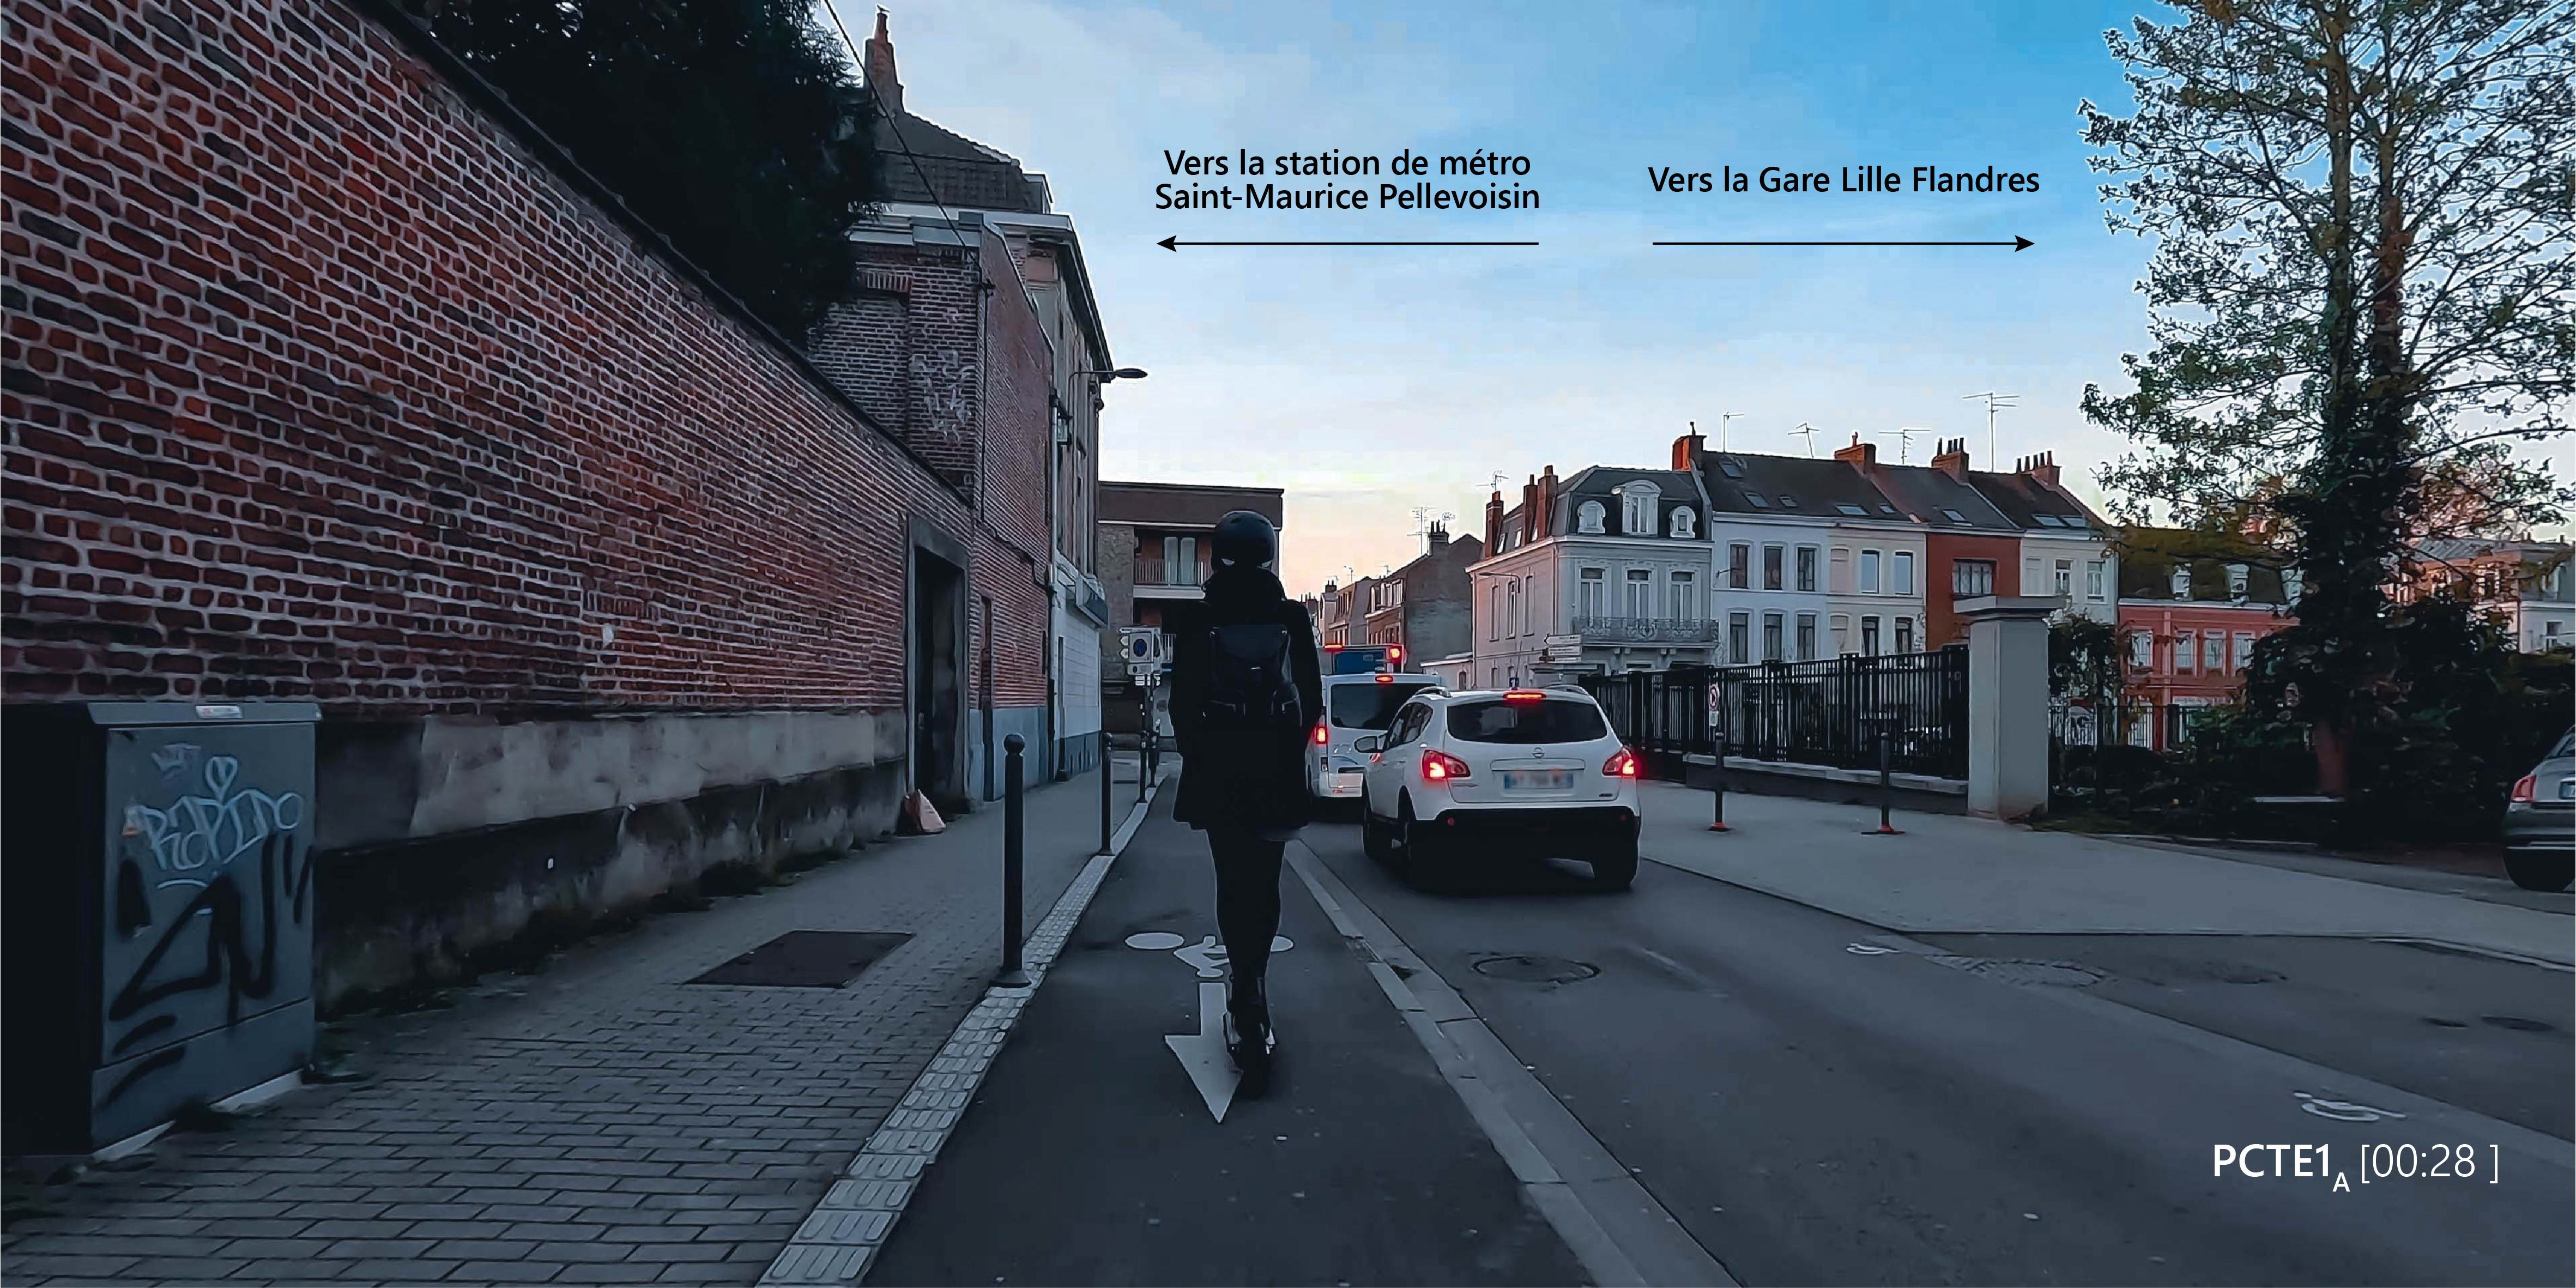
\includegraphics[width=0.75\columnwidth]{src/Figures/Annexes/Extrait_Video_PCTE1_Access_1.jpg}}
        \vspace{5pt}
        \begin{flushright}\scriptsize{
        Auteur~: \textcolor{blue}{Dylan Moinse (2022)}
        }\end{flushright}
    \end{figure}

    % PCTE1 Photo Access 2
    \begin{figure}[h!]\vspace*{4pt}
        \caption*{Extrait n°2 de la vidéo lors du trajet en rabattement (\(PCTE^{A}_{1}\))}
        \centerline{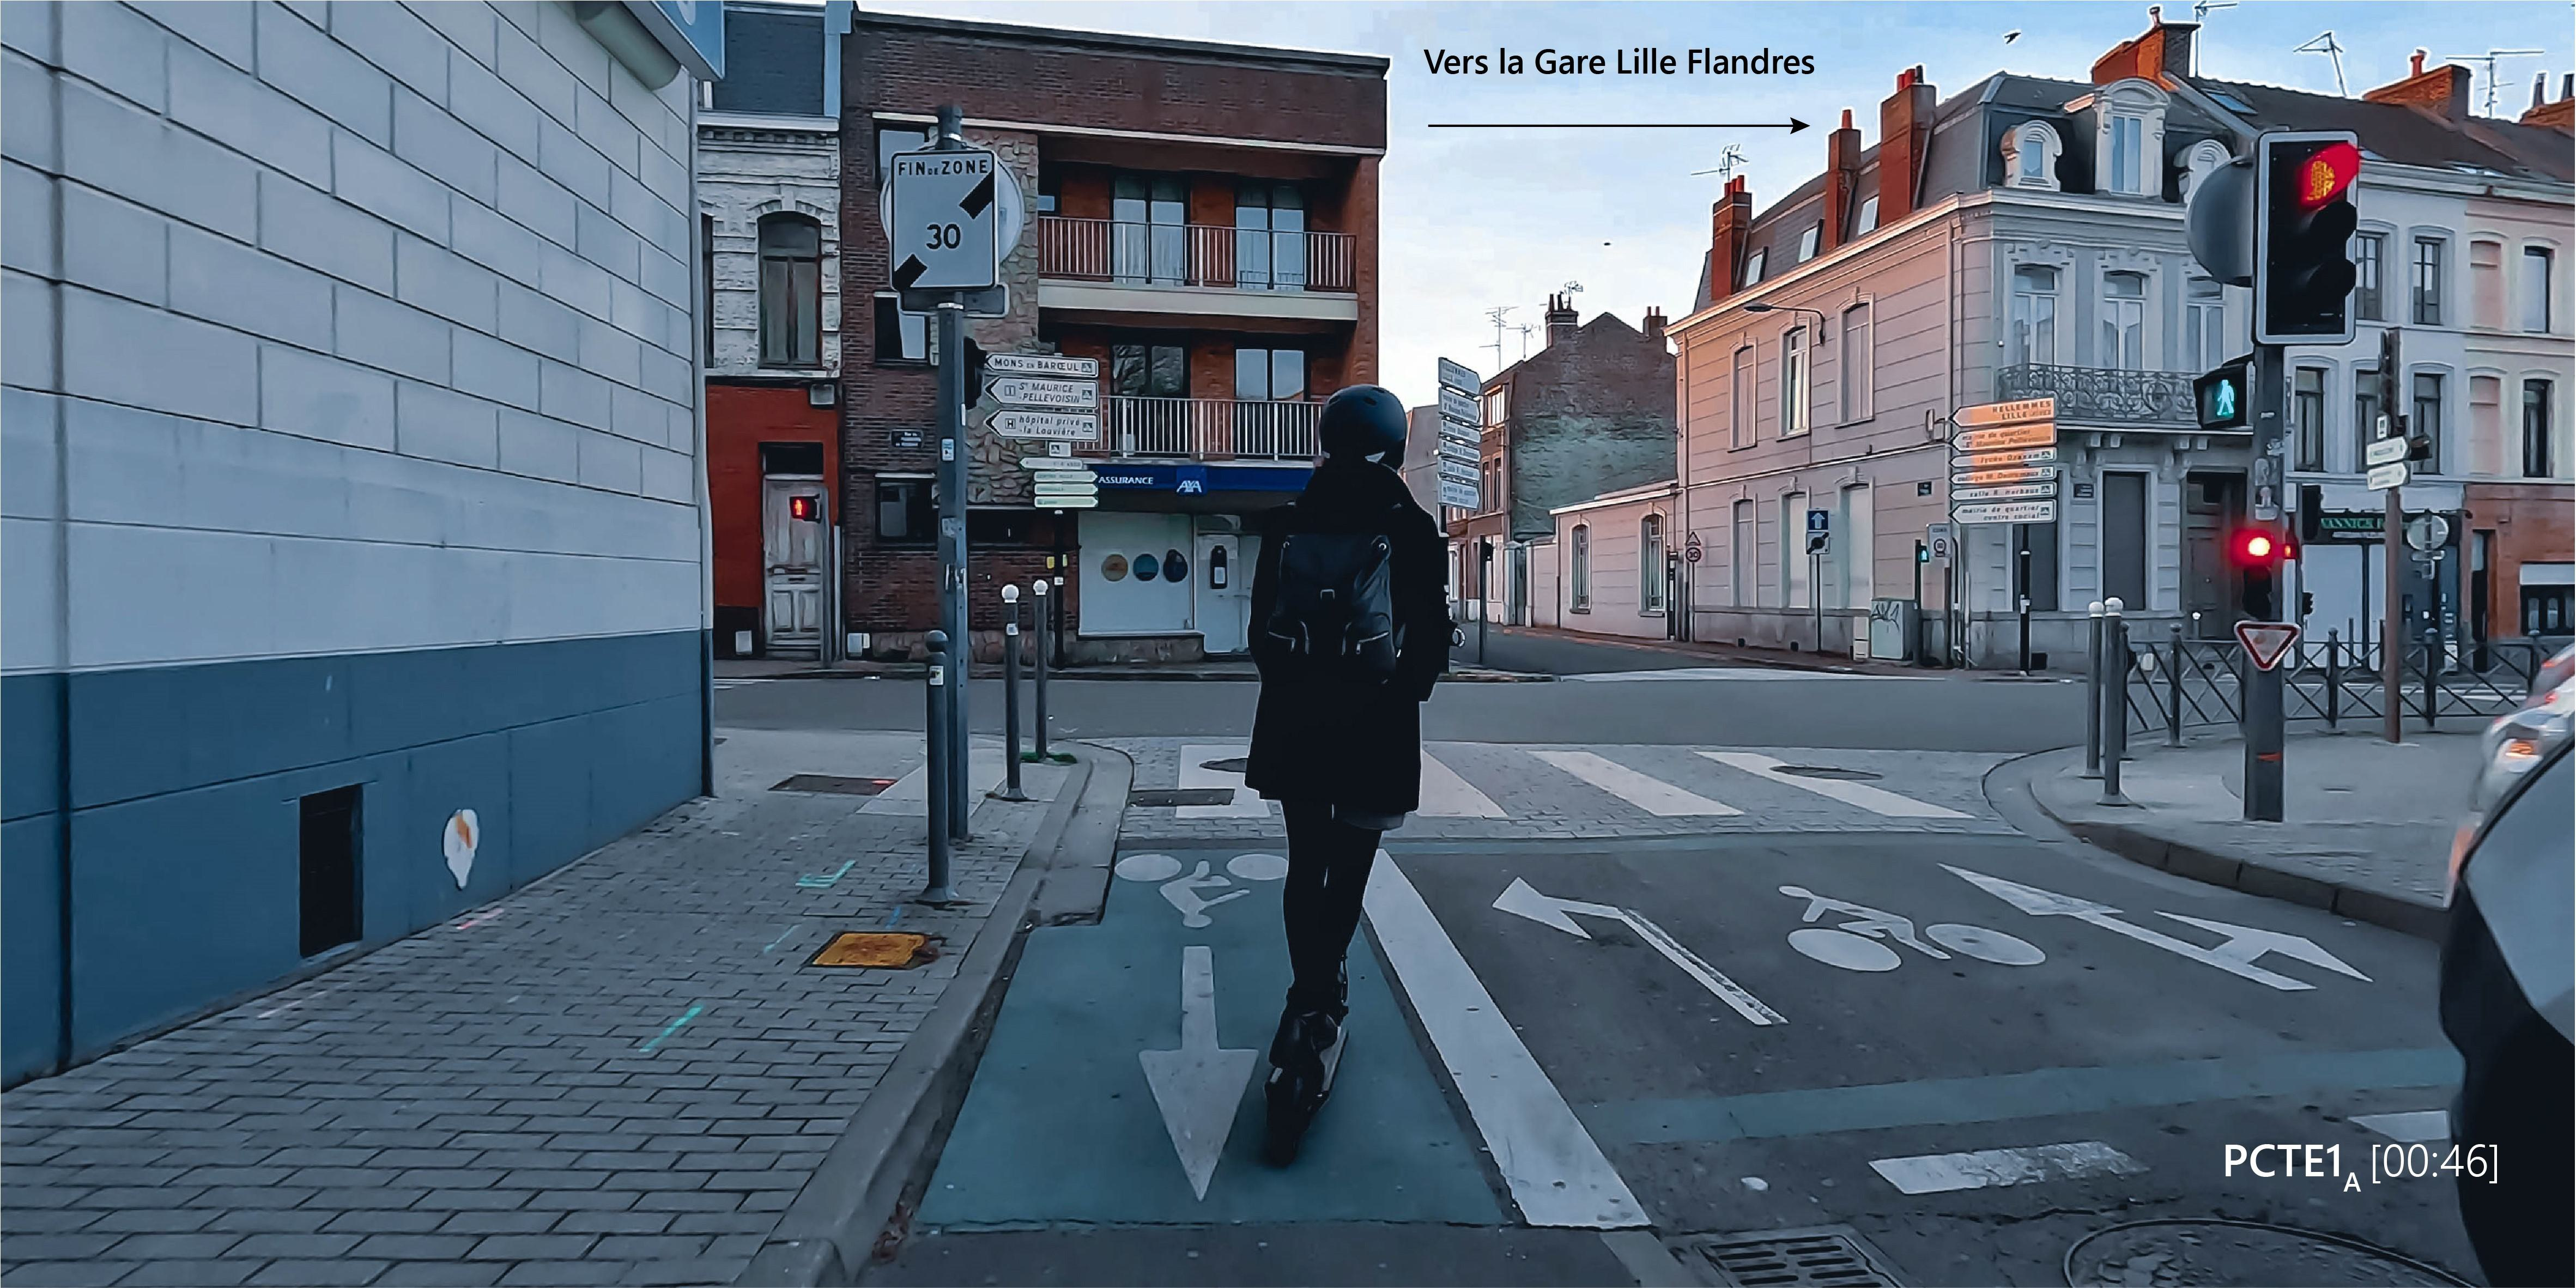
\includegraphics[width=0.75\columnwidth]{src/Figures/Annexes/Extrait_Video_PCTE1_Access_2.jpg}}
        \vspace{5pt}
        \begin{flushright}\scriptsize{
        Auteur~: \textcolor{blue}{Dylan Moinse (2022)}
        }\end{flushright}
    \end{figure}

    % PCTE1 Photo Access 3
    \begin{figure}[h!]\vspace*{4pt}
        \caption*{Extrait n°3 de la vidéo lors du trajet en rabattement (\(PCTE^{A}_{1}\))}
        \centerline{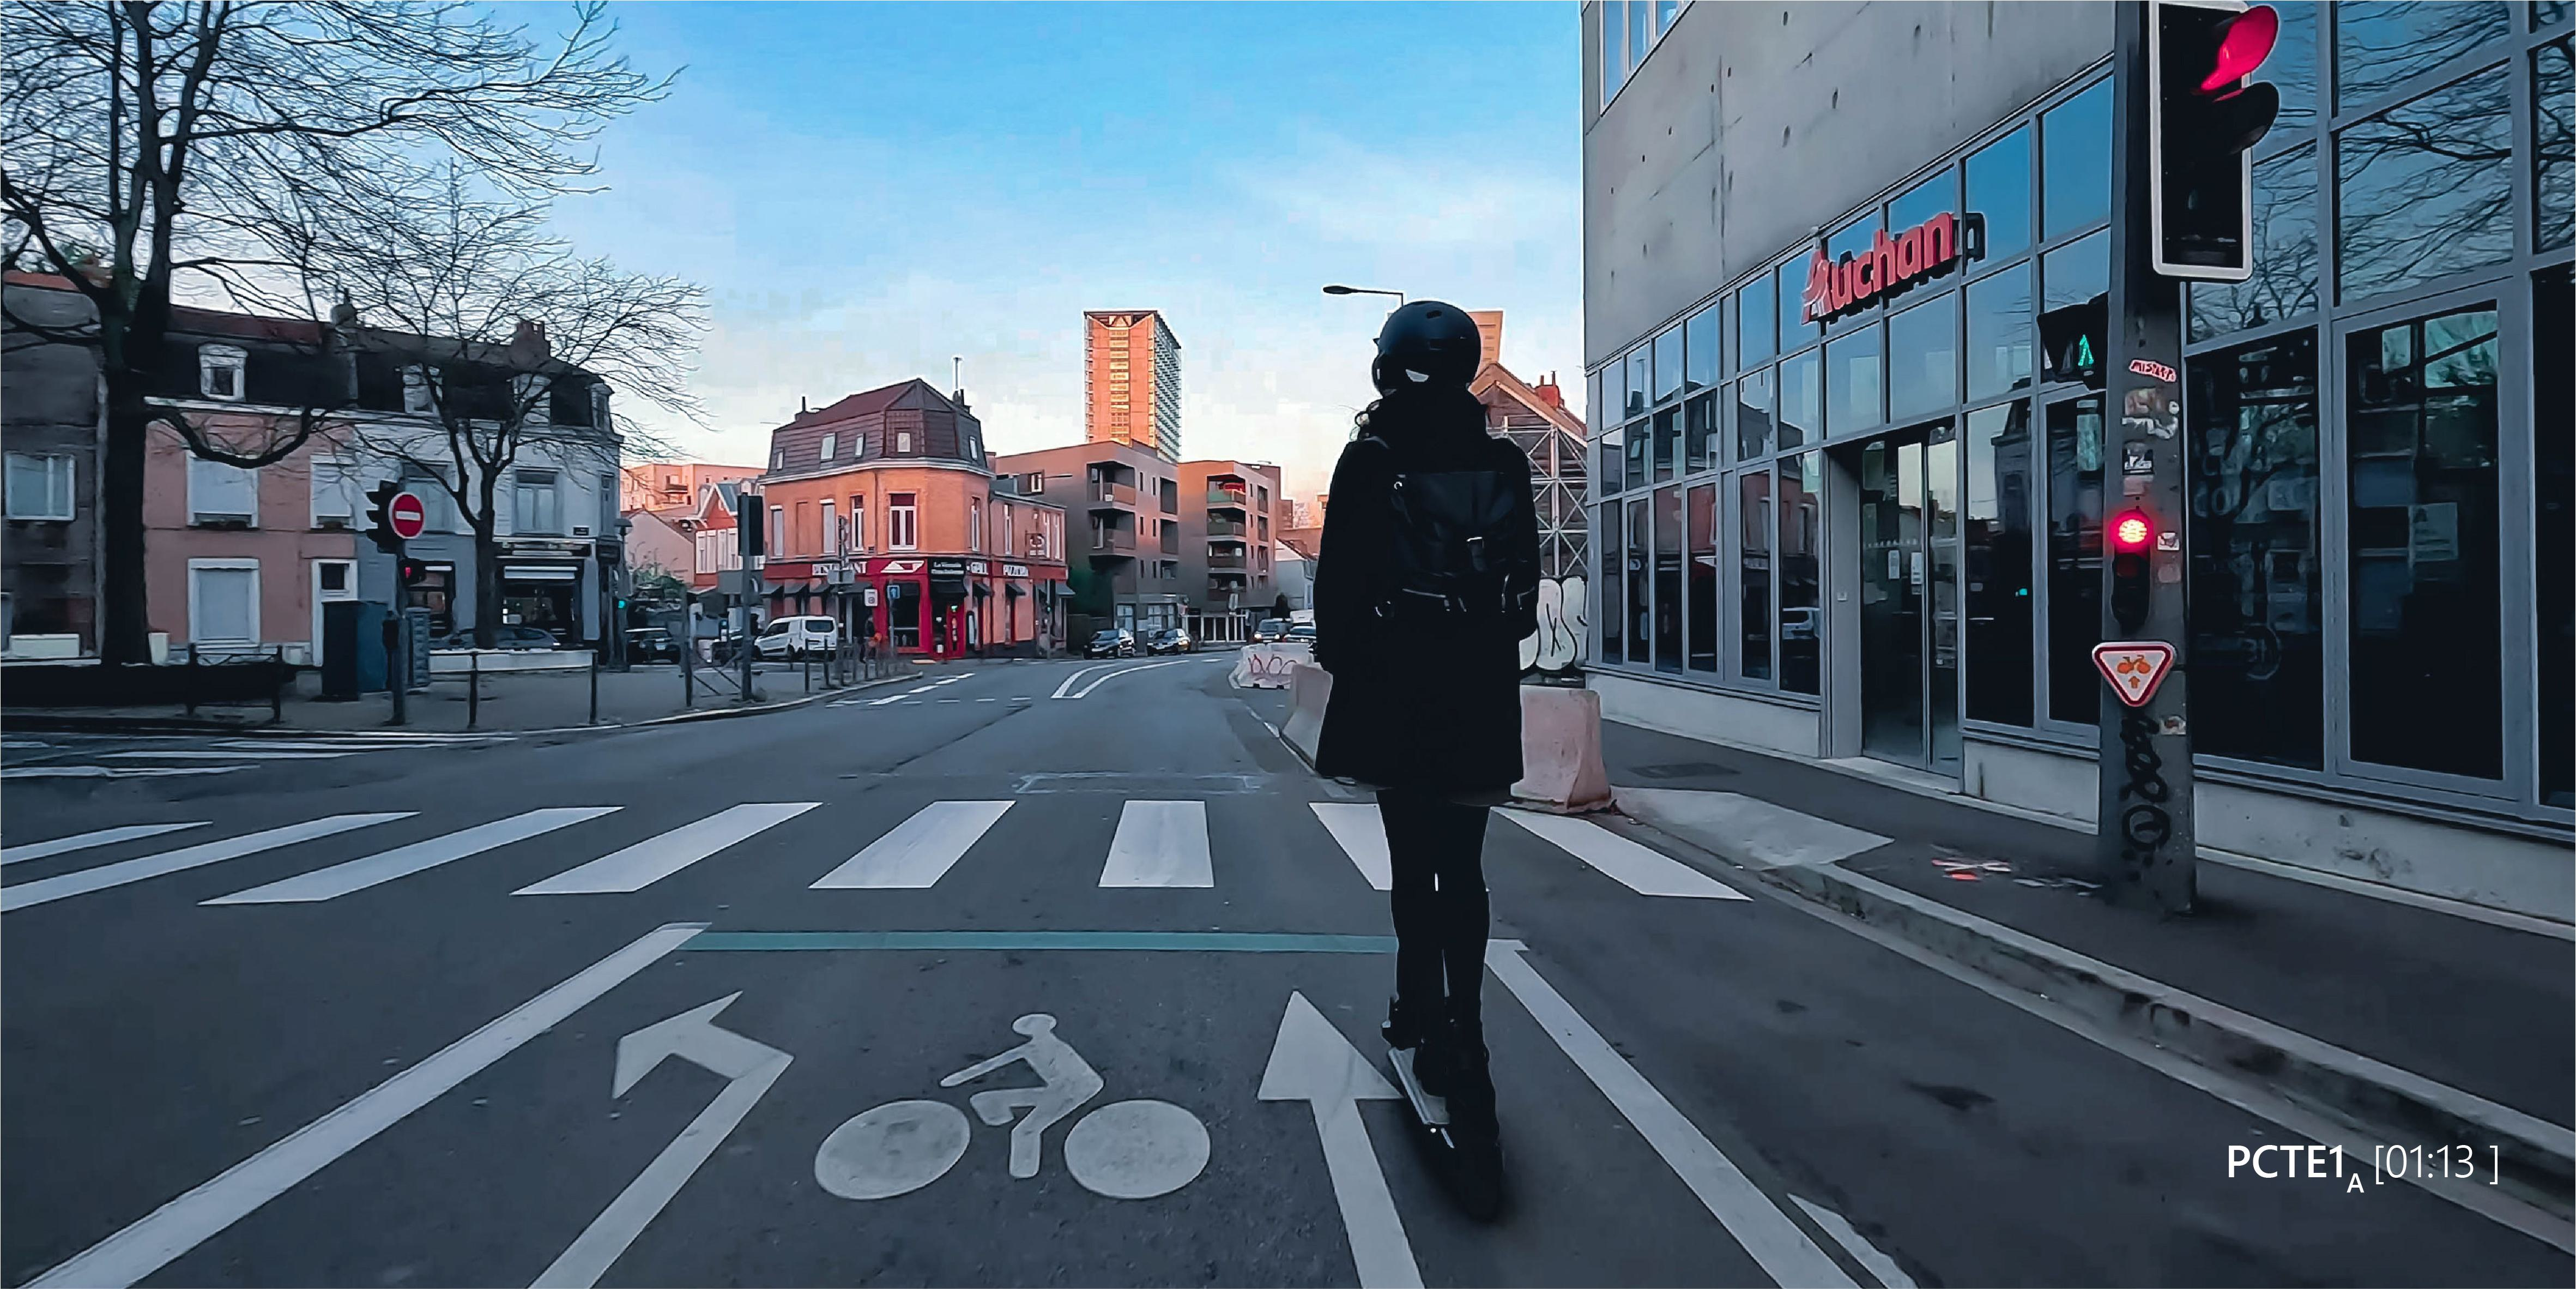
\includegraphics[width=0.75\columnwidth]{src/Figures/Annexes/Extrait_Video_PCTE1_Access_3.jpg}}
        \vspace{5pt}
        \begin{flushright}\scriptsize{
        Auteur~: \textcolor{blue}{Dylan Moinse (2022)}
        }\end{flushright}
    \end{figure}

    % PCTE1 Photo Access 4
    \begin{figure}[h!]\vspace*{4pt}
        \caption*{Extrait n°4 de la vidéo lors du trajet en rabattement (\(PCTE^{A}_{1}\))}
        \centerline{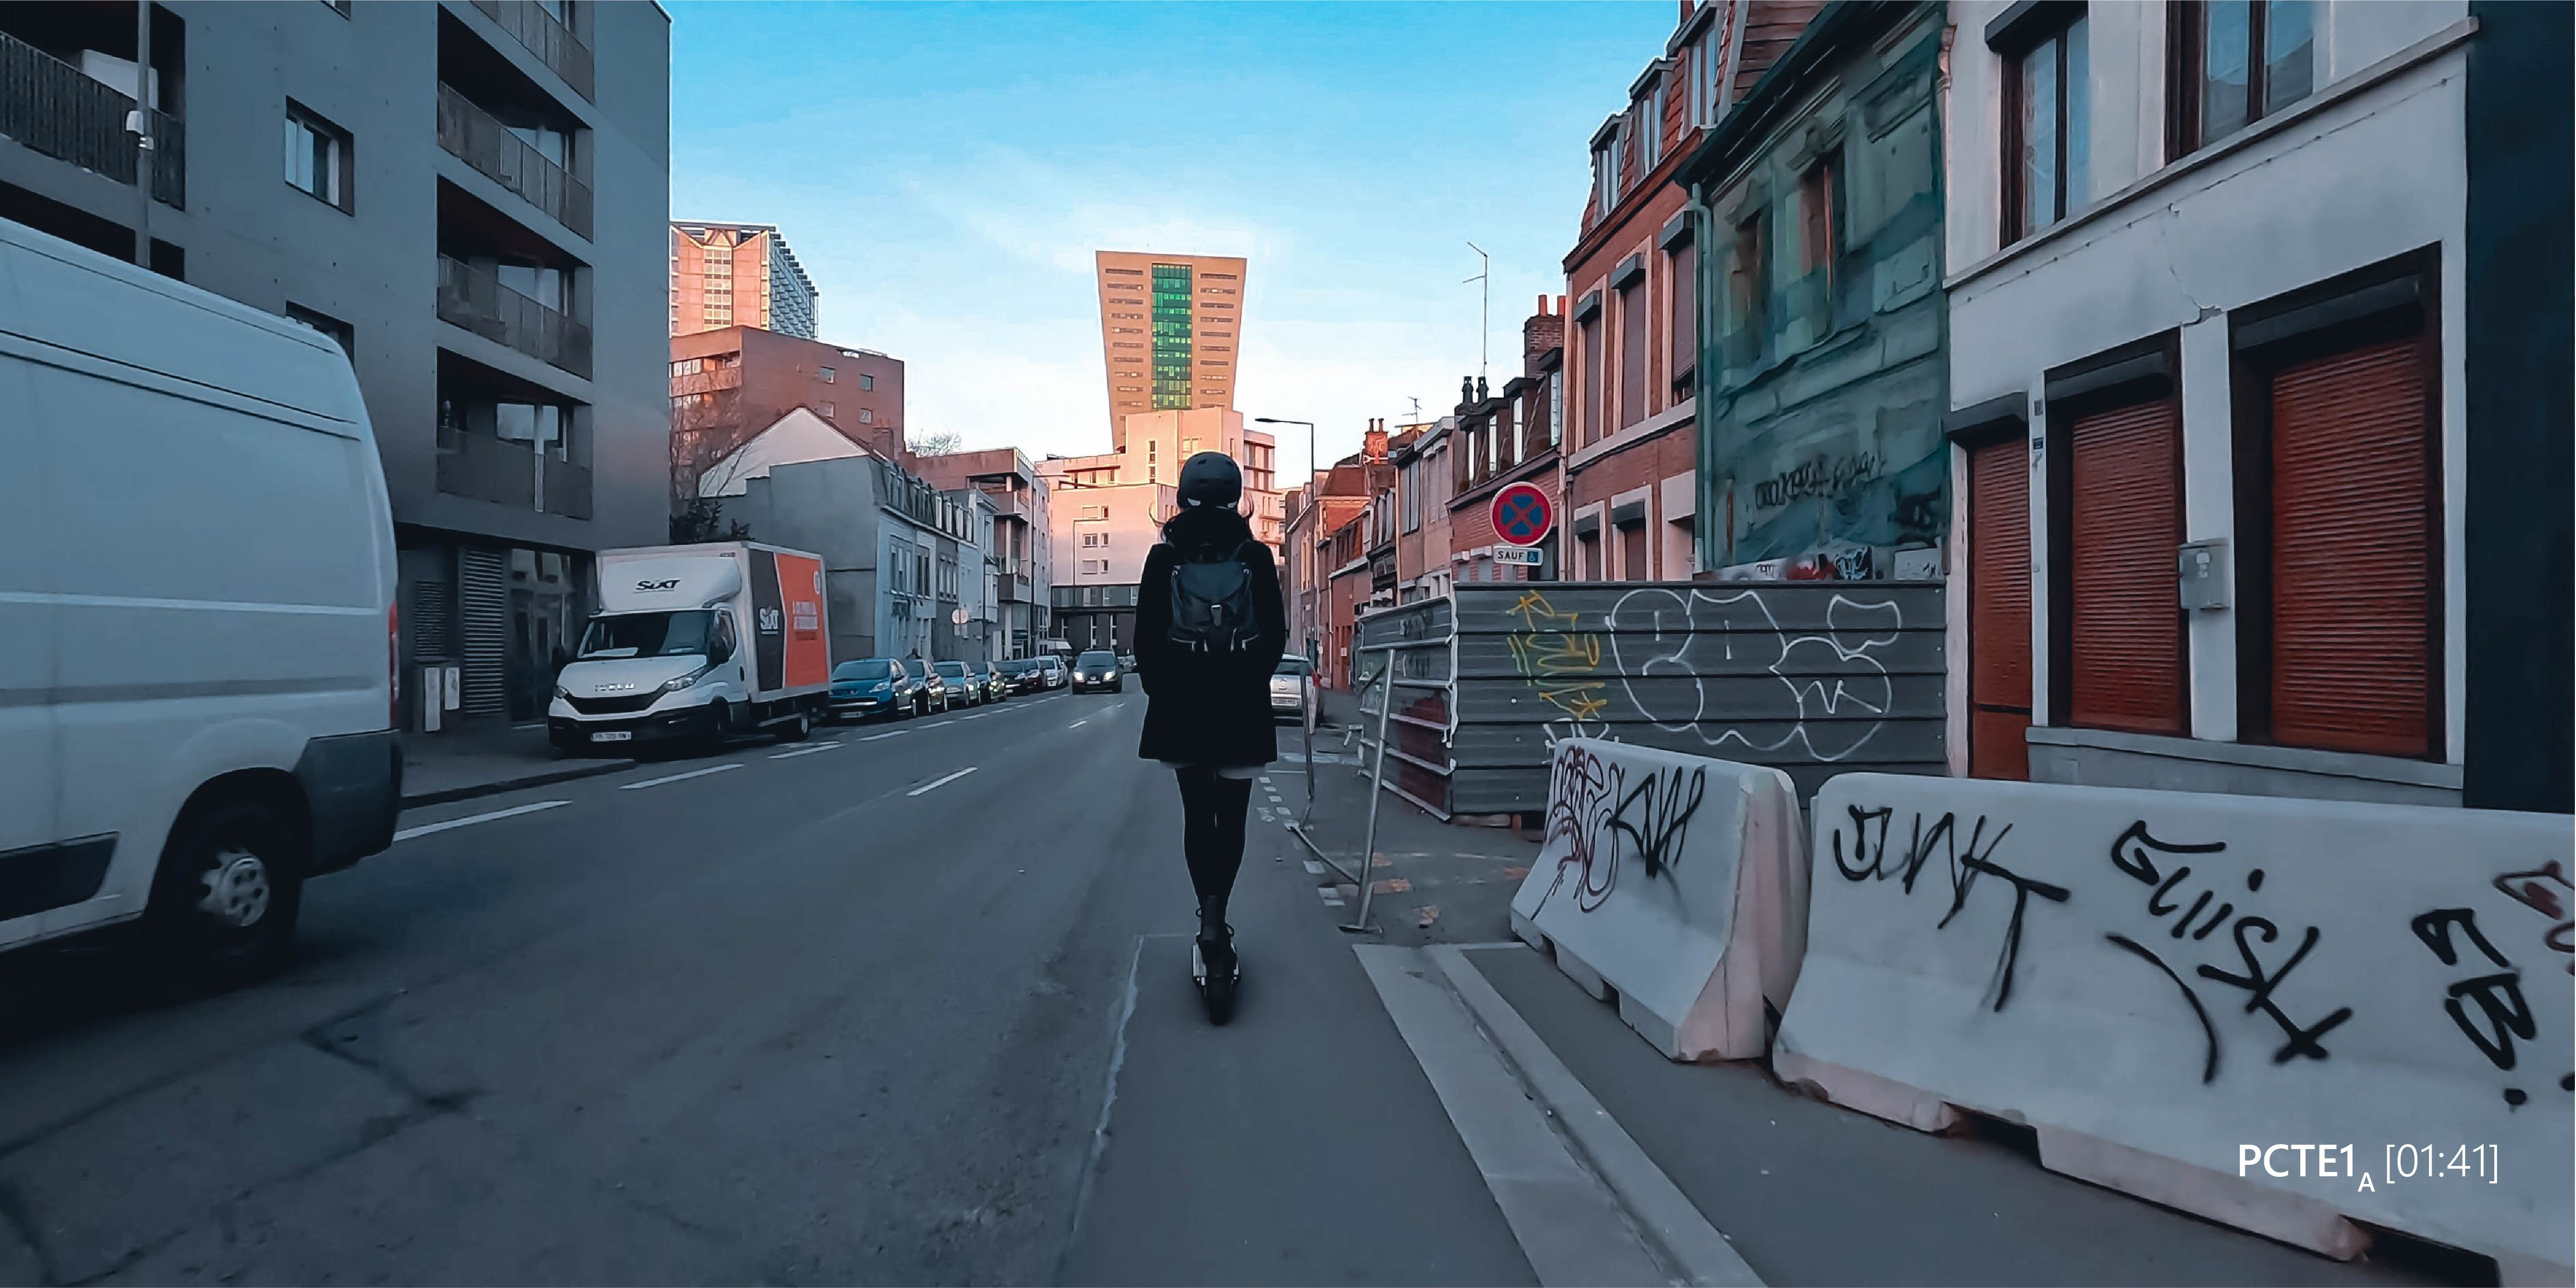
\includegraphics[width=0.75\columnwidth]{src/Figures/Annexes/Extrait_Video_PCTE1_Access_4.jpg}}
        \vspace{5pt}
        \begin{flushright}\scriptsize{
        Auteur~: \textcolor{blue}{Dylan Moinse (2022)}
        }\end{flushright}
    \end{figure}

    % PCTE1 Photo Access 5
    \begin{figure}[h!]\vspace*{4pt}
        \caption*{Extrait n°5 de la vidéo lors du trajet en rabattement (\(PCTE^{A}_{1}\))}
        \centerline{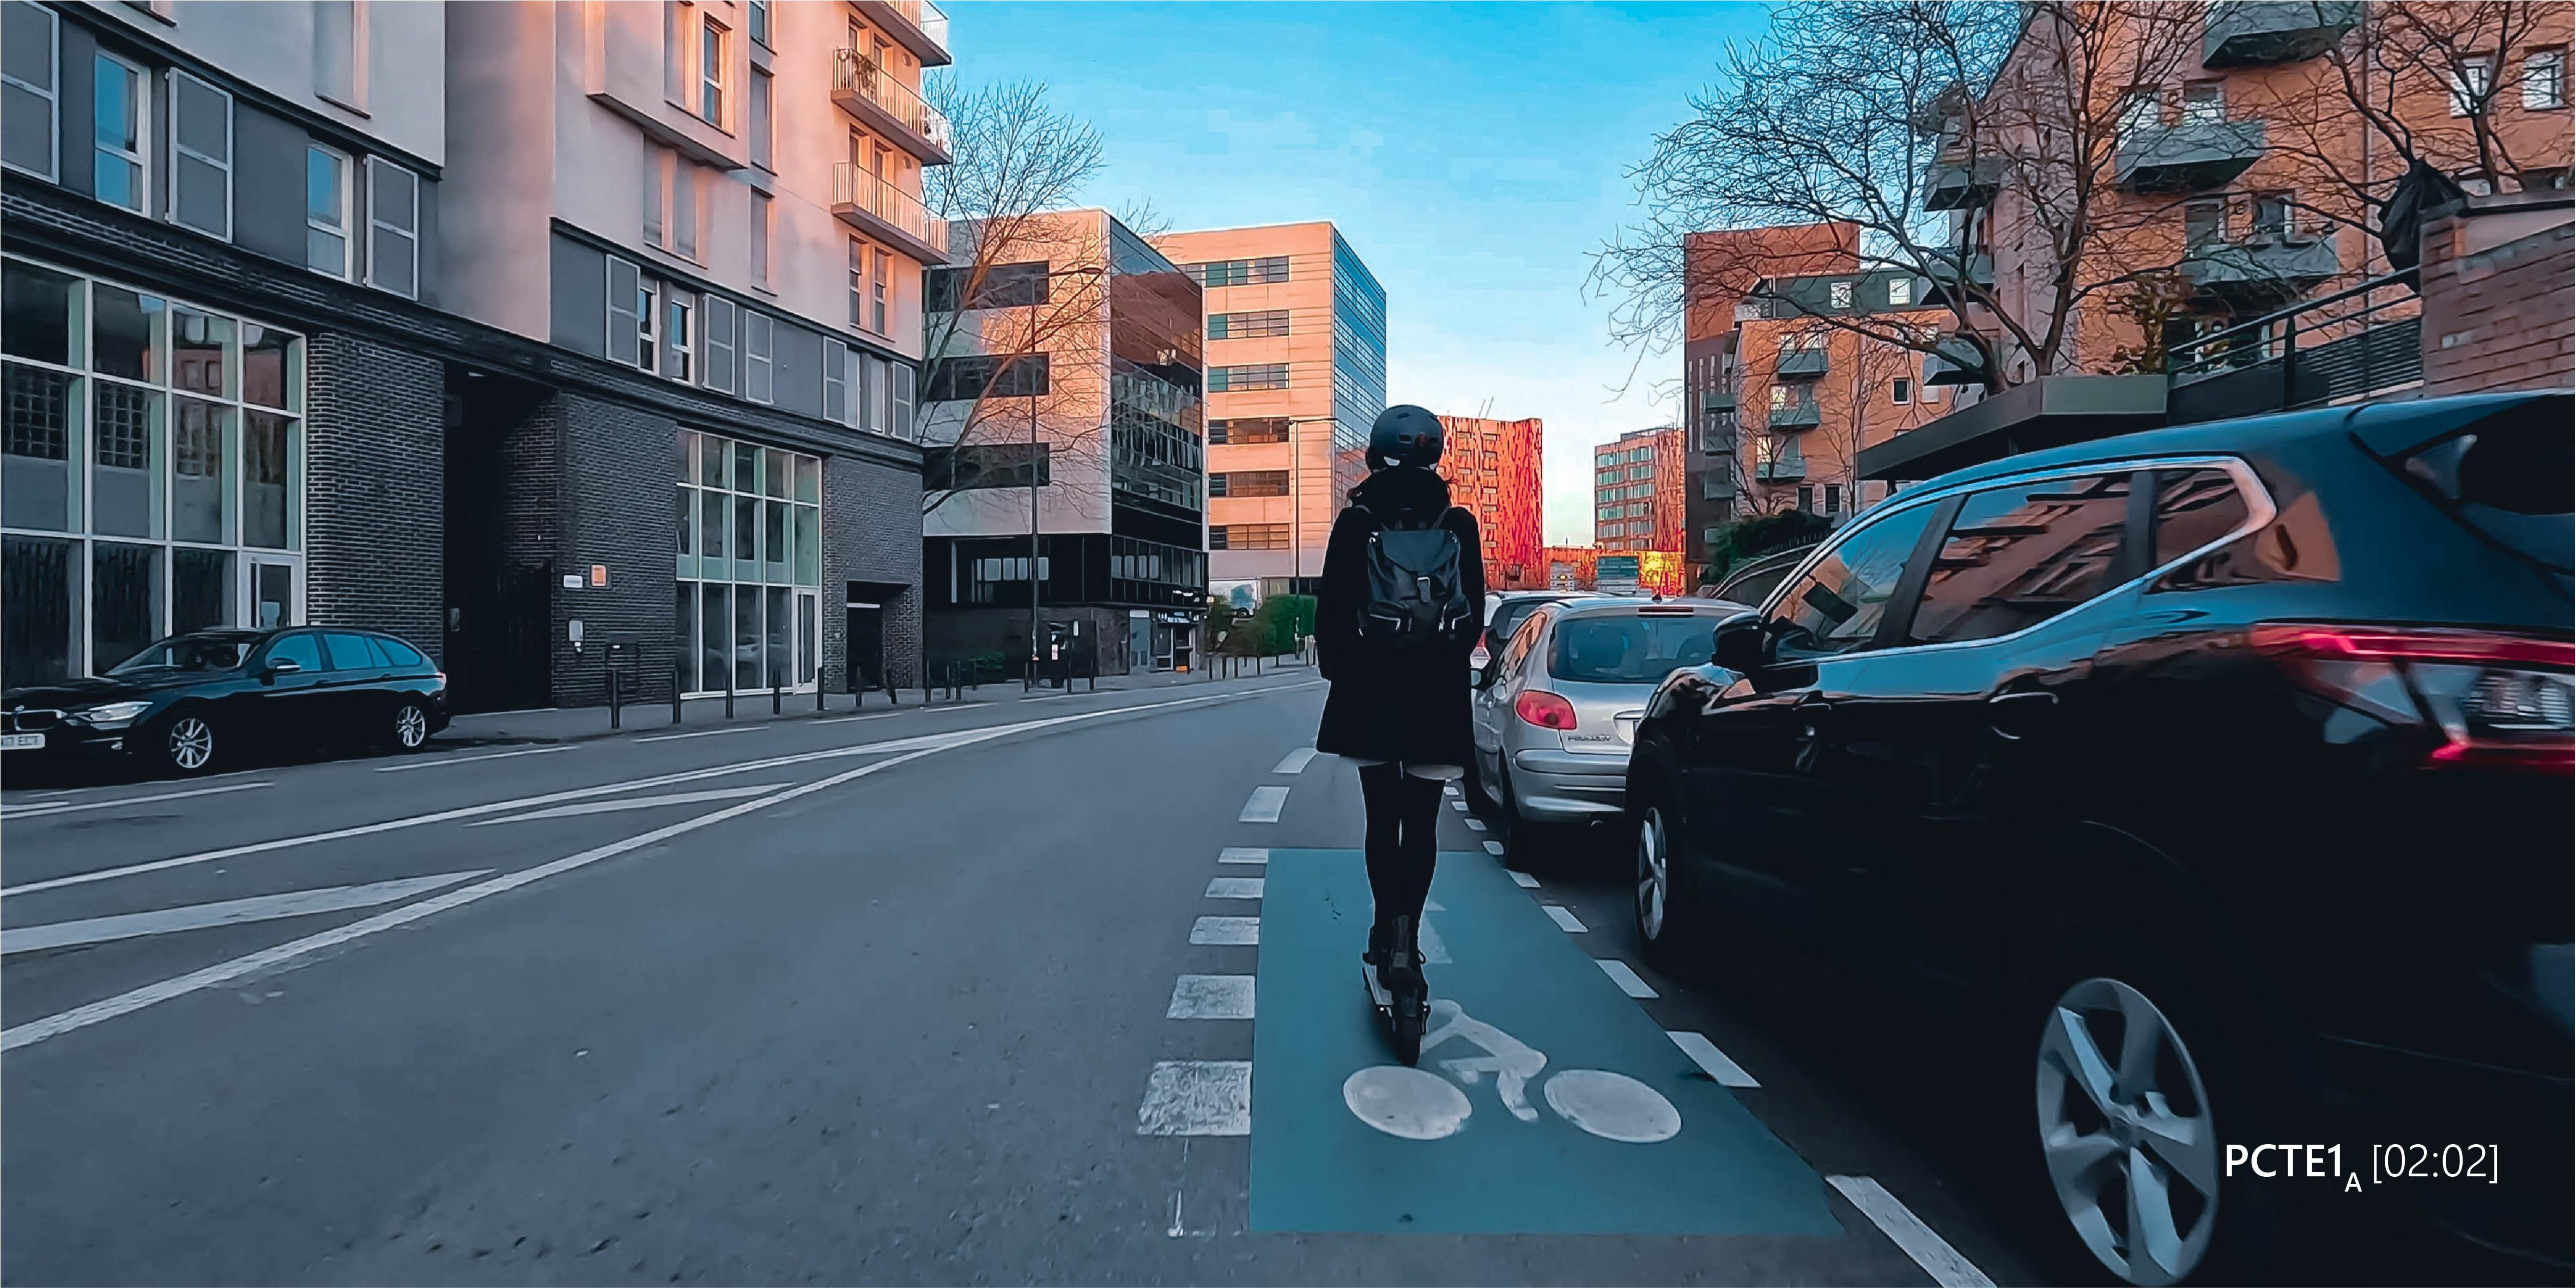
\includegraphics[width=0.75\columnwidth]{src/Figures/Annexes/Extrait_Video_PCTE1_Access_5.jpg}}
        \vspace{5pt}
        \begin{flushright}\scriptsize{
        Auteur~: \textcolor{blue}{Dylan Moinse (2022)}
        }\end{flushright}
    \end{figure}

    % PCTE1 Photo Access 6
    \begin{figure}[h!]\vspace*{4pt}
        \caption*{Extrait n°6 de la vidéo lors du trajet en rabattement (\(PCTE^{A}_{1}\))}
        \centerline{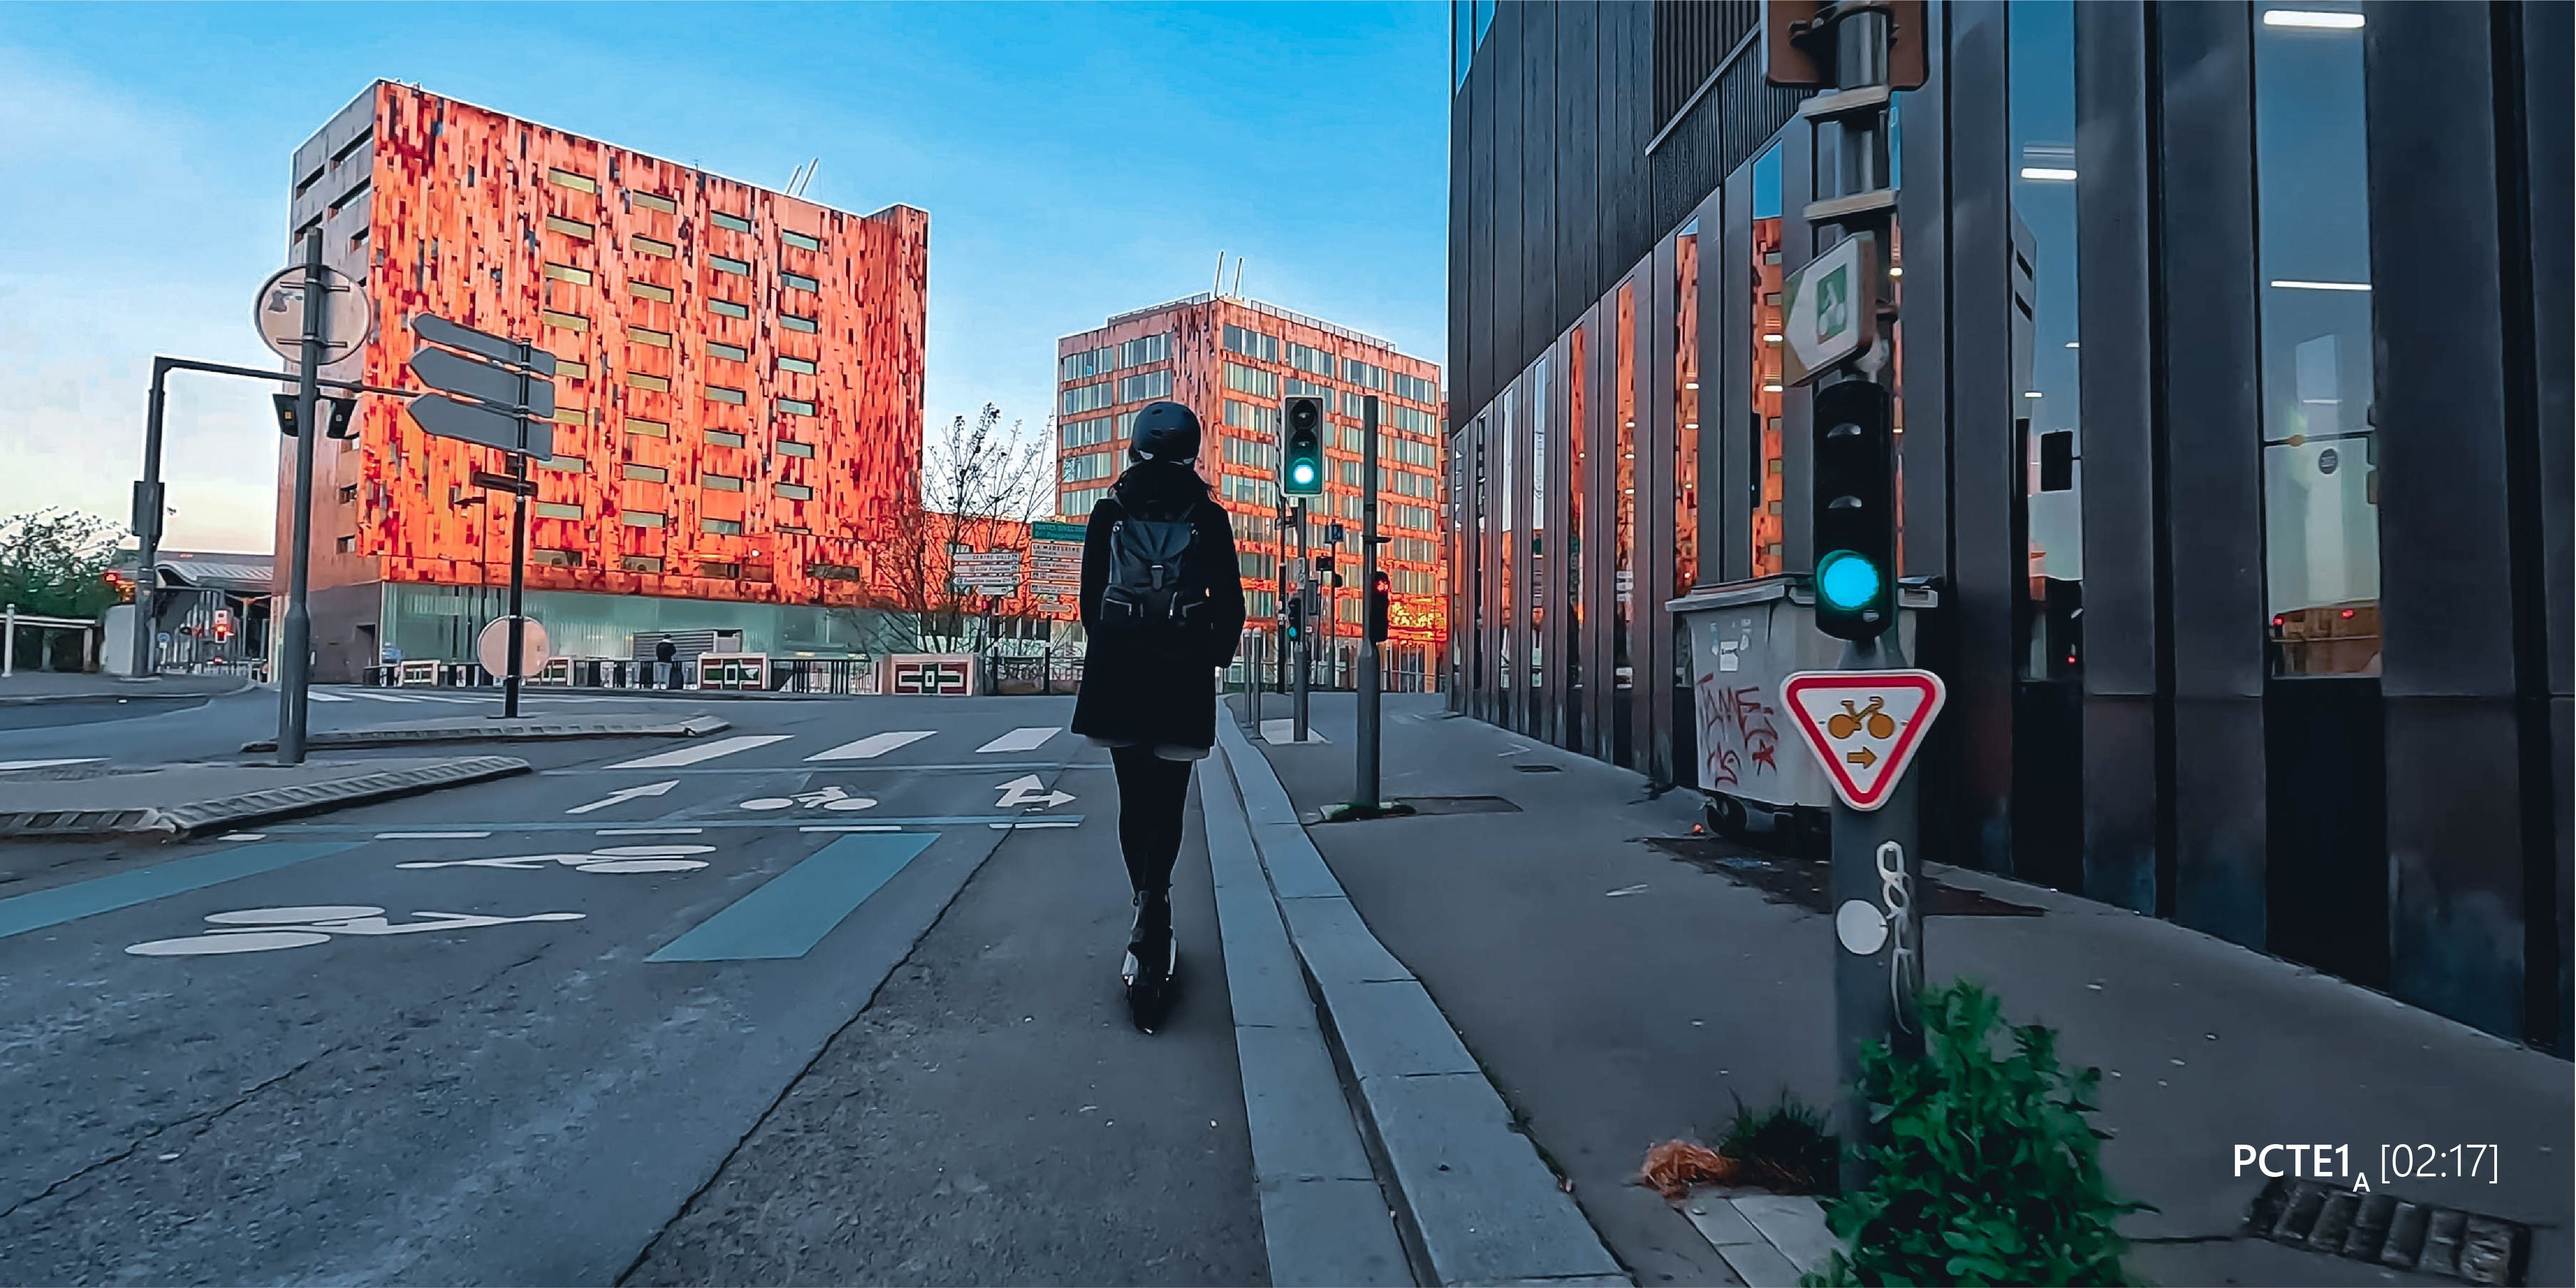
\includegraphics[width=0.75\columnwidth]{src/Figures/Annexes/Extrait_Video_PCTE1_Access_6.jpg}}
        \vspace{5pt}
        \begin{flushright}\scriptsize{
        Auteur~: \textcolor{blue}{Dylan Moinse (2022)}
        }\end{flushright}
    \end{figure}

    % PCTE1 Photo Access 7
    \begin{figure}[h!]\vspace*{4pt}
        \caption*{Extrait n°7 de la vidéo lors du trajet en rabattement (\(PCTE^{A}_{1}\))}
        \centerline{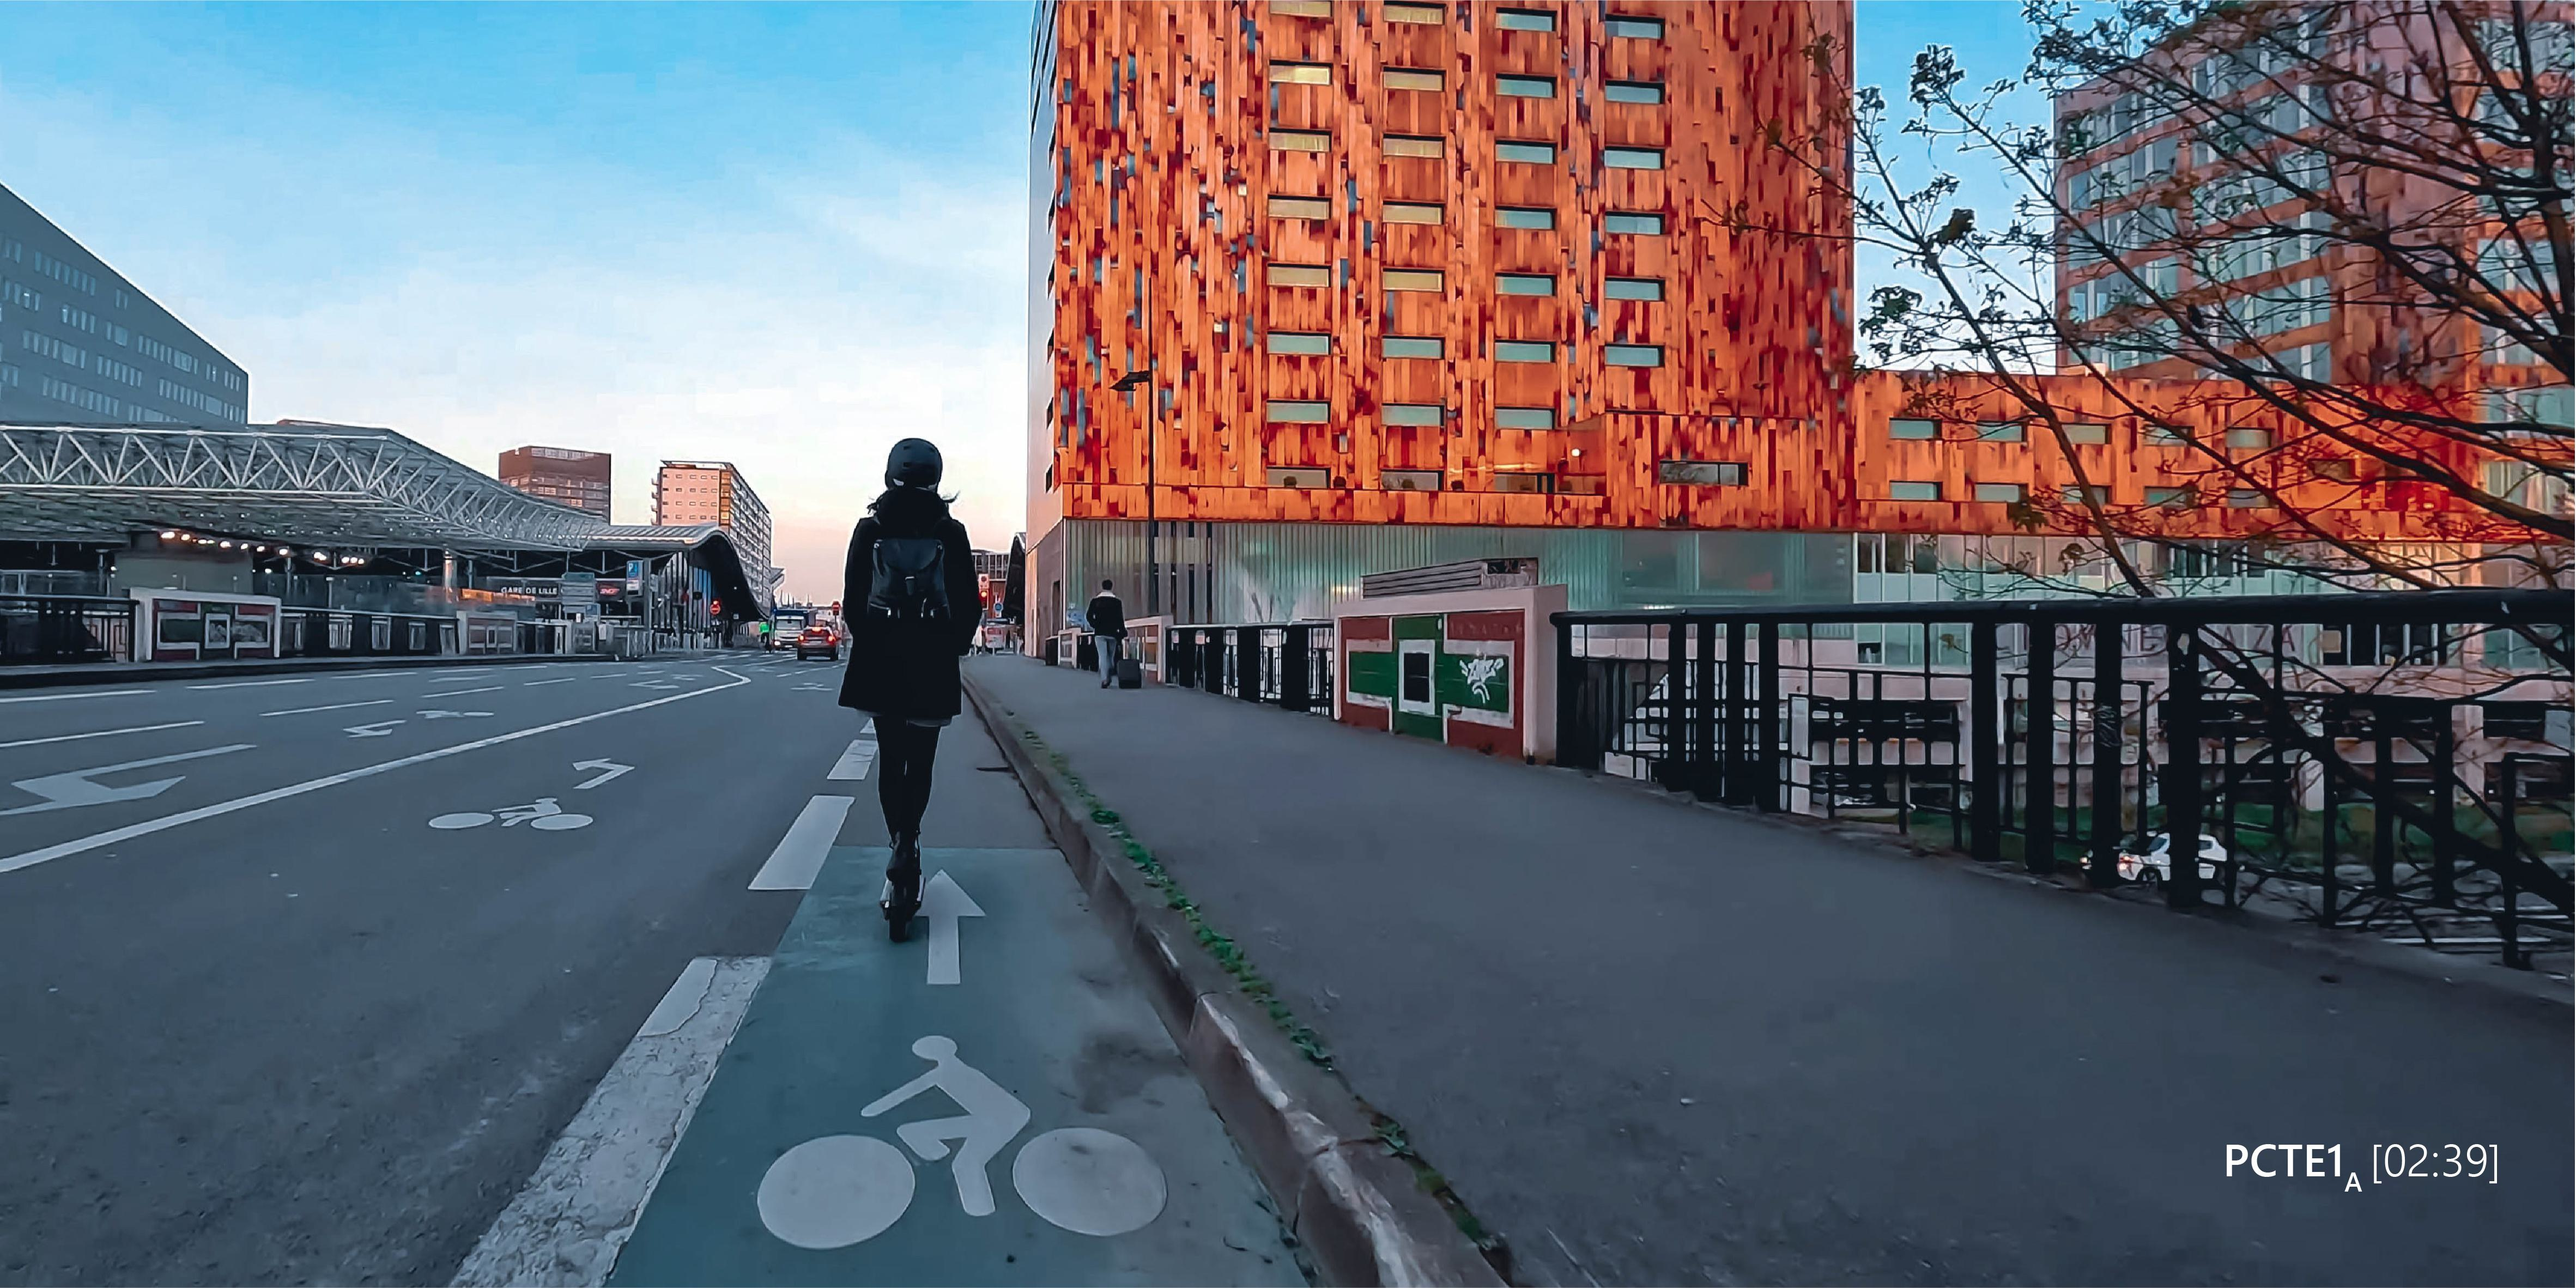
\includegraphics[width=0.75\columnwidth]{src/Figures/Annexes/Extrait_Video_PCTE1_Access_7.jpg}}
        \vspace{5pt}
        \begin{flushright}\scriptsize{
        Auteur~: \textcolor{blue}{Dylan Moinse (2022)}
        }\end{flushright}
    \end{figure}

    % PCTE1 Photo Access 8
    \begin{figure}[h!]\vspace*{4pt}
        \caption*{Extrait n°8 de la vidéo lors du trajet en rabattement (\(PCTE^{A}_{1}\))}
        \centerline{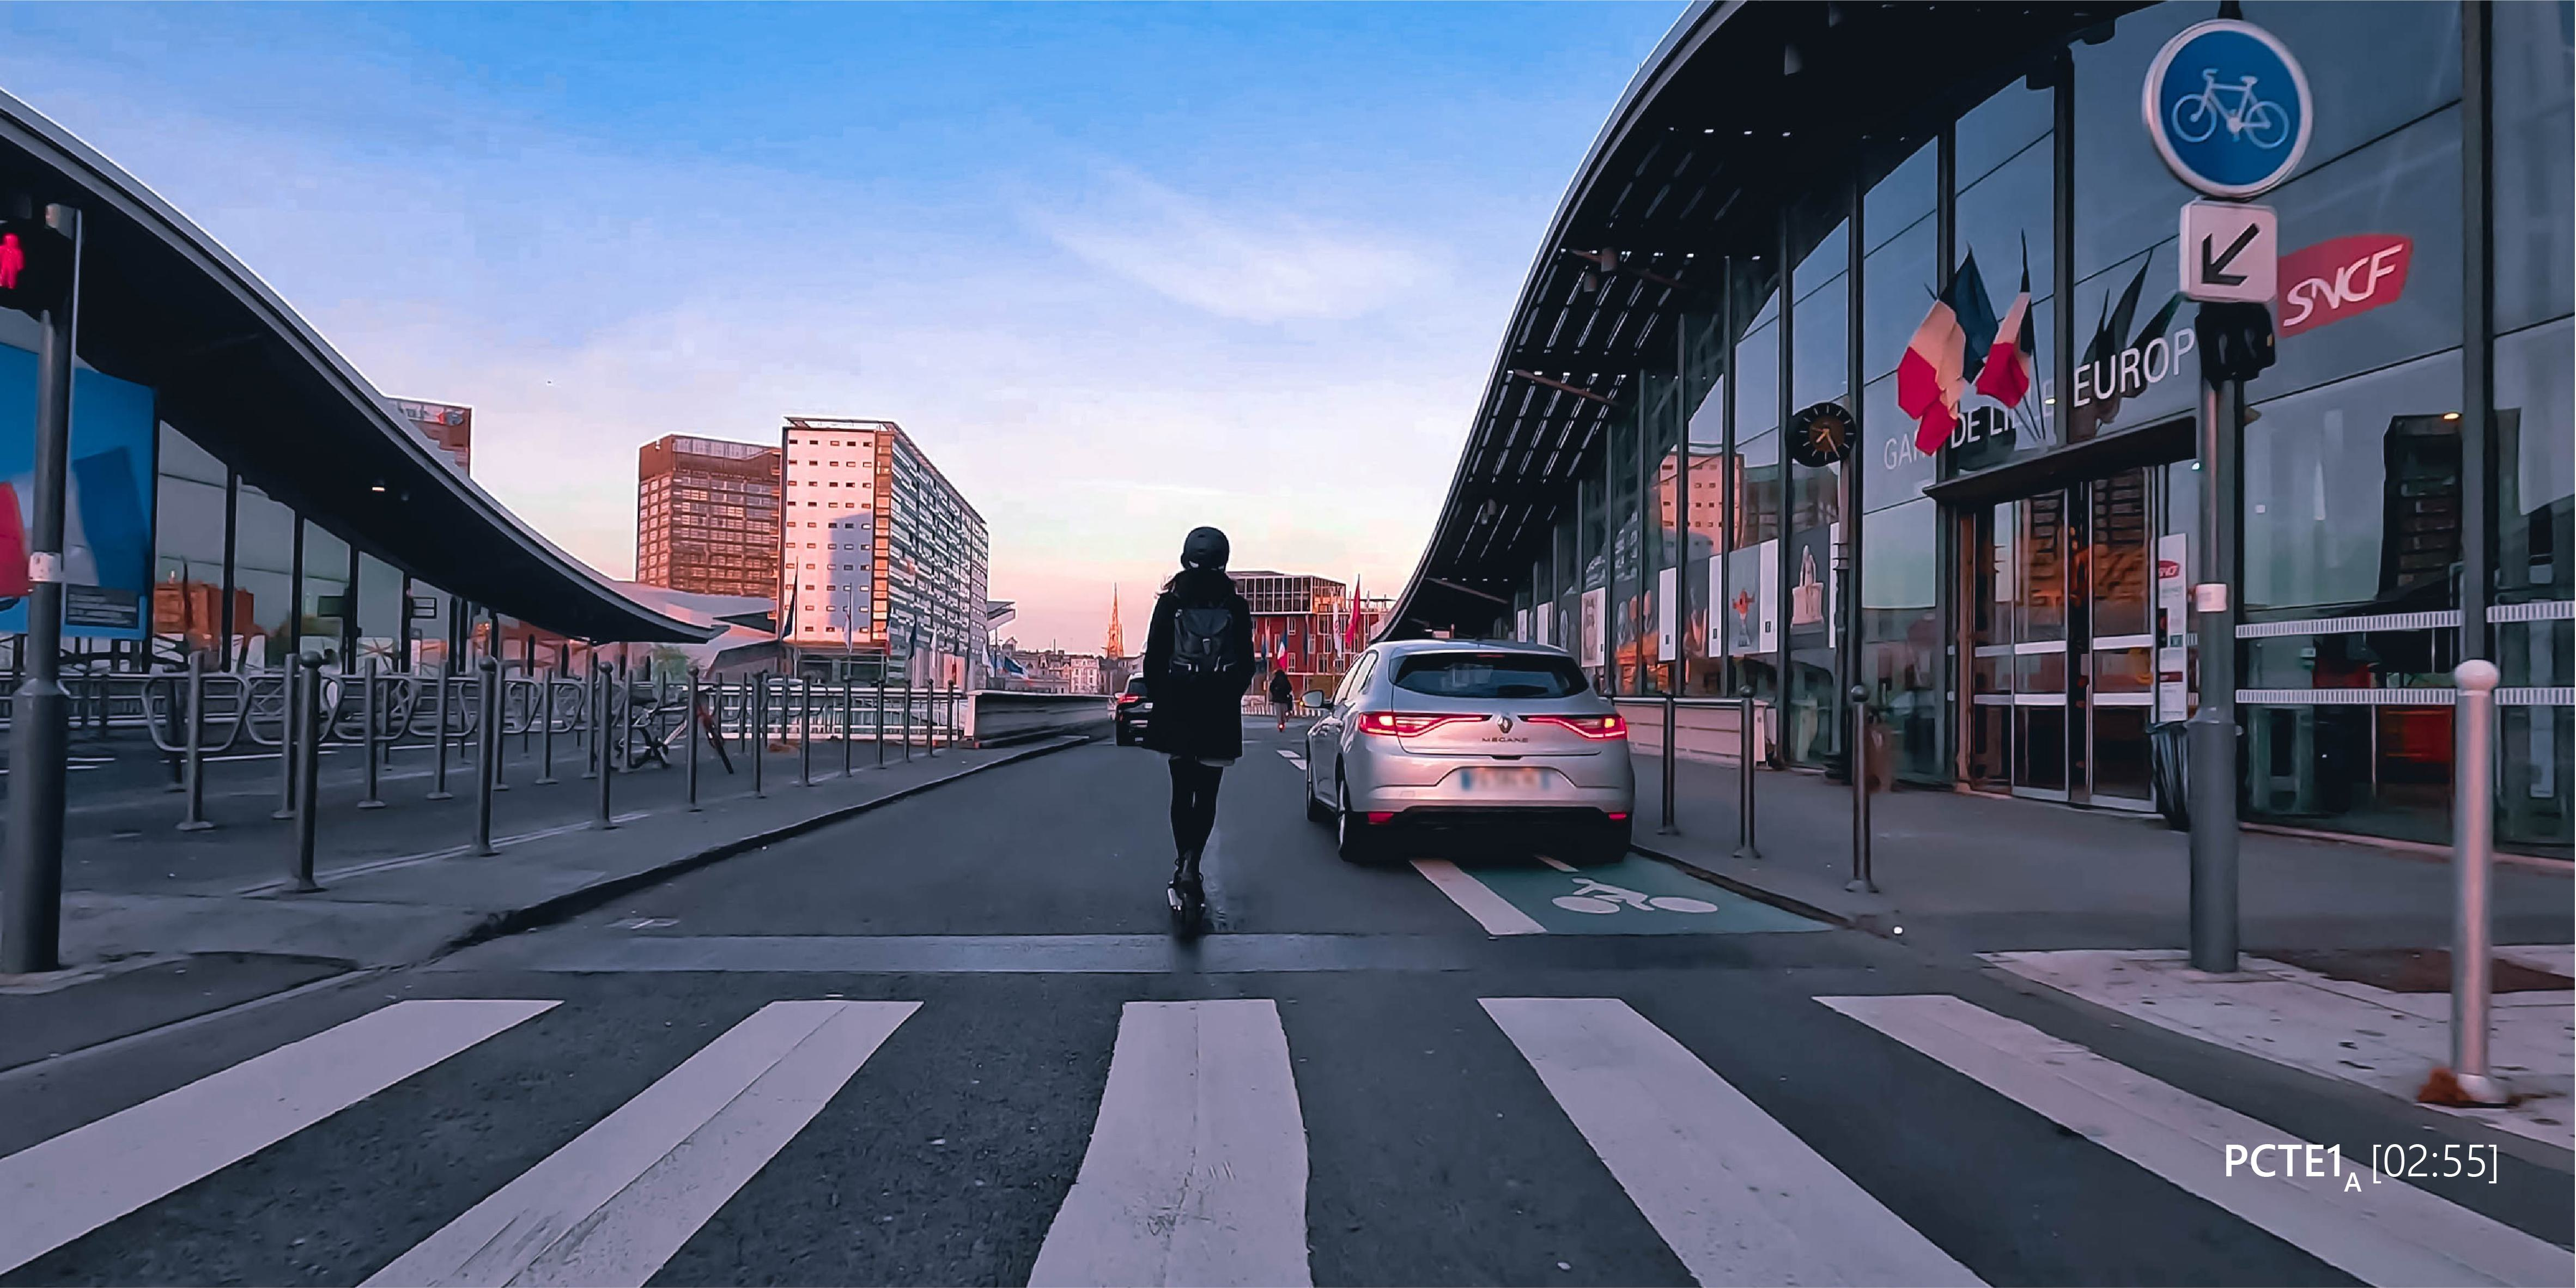
\includegraphics[width=0.75\columnwidth]{src/Figures/Annexes/Extrait_Video_PCTE1_Access_8.jpg}}
        \vspace{5pt}
        \begin{flushright}\scriptsize{
        Auteur~: \textcolor{blue}{Dylan Moinse (2022)}
        }\end{flushright}
    \end{figure}

    % PCTE1 Photo Access 9
    \begin{figure}[h!]\vspace*{4pt}
        \caption*{Extrait n°9 de la vidéo lors du trajet en rabattement (\(PCTE^{A}_{1}\))}
        \centerline{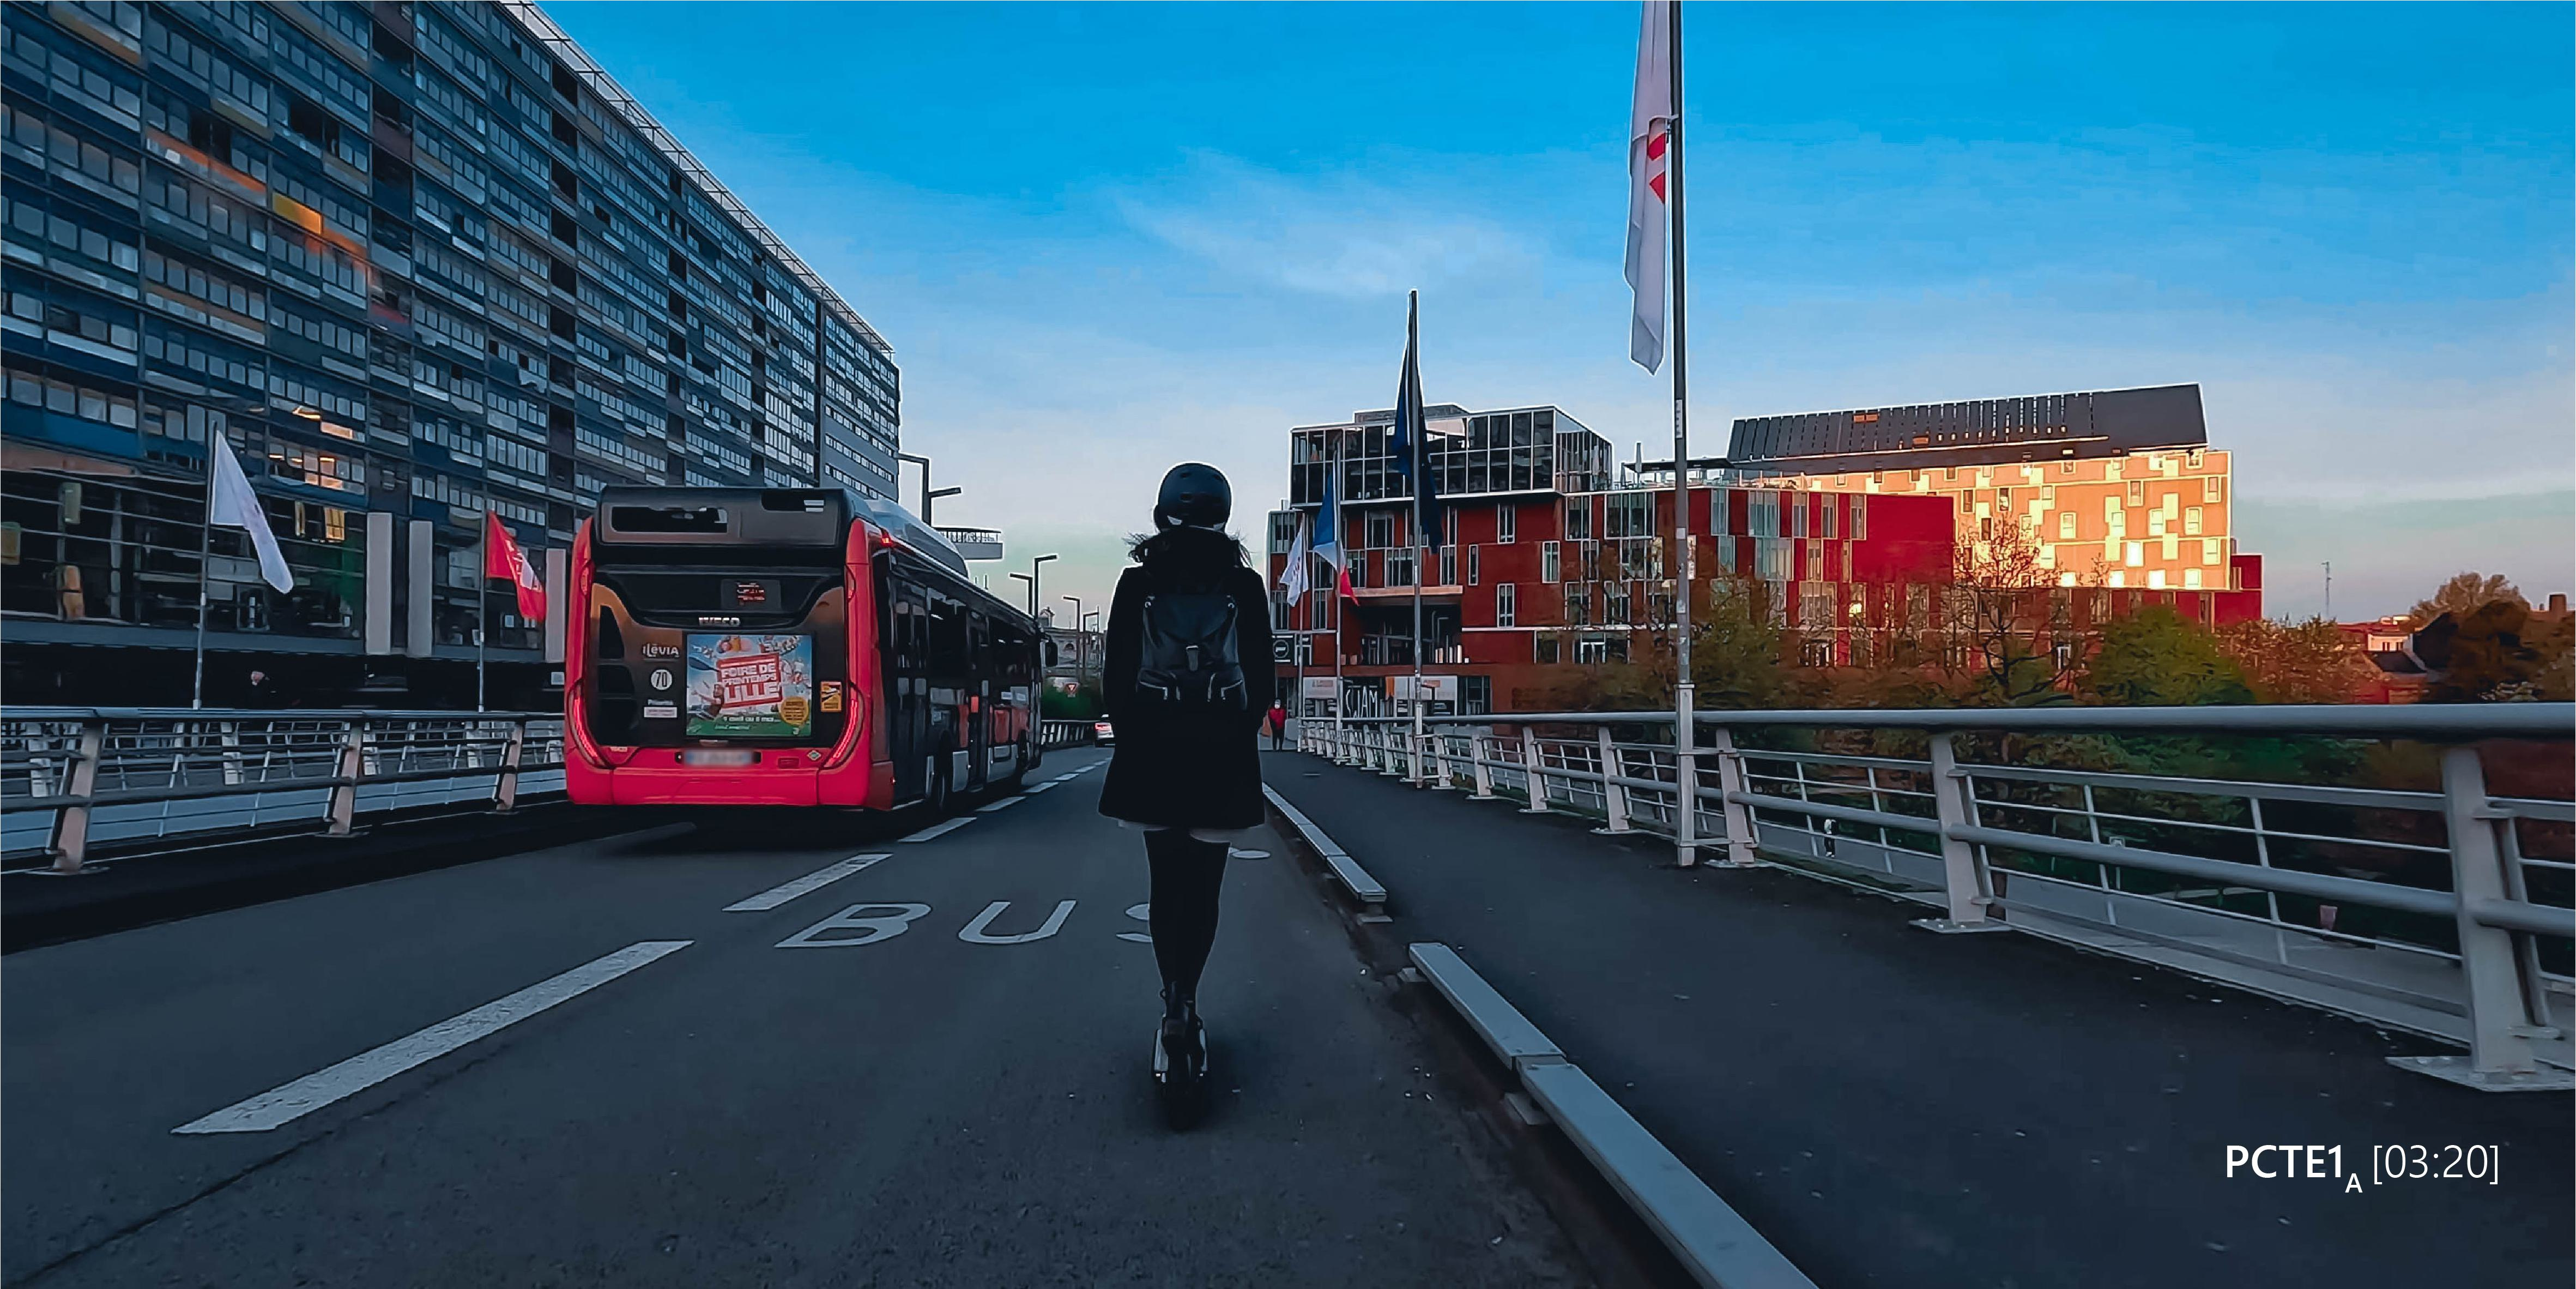
\includegraphics[width=0.75\columnwidth]{src/Figures/Annexes/Extrait_Video_PCTE1_Access_9.jpg}}
        \vspace{5pt}
        \begin{flushright}\scriptsize{
        Auteur~: \textcolor{blue}{Dylan Moinse (2022)}
        }\end{flushright}
    \end{figure}

    % PCTE1 Photo Access 10
    \begin{figure}[h!]\vspace*{4pt}
        \caption*{Extrait n°10 de la vidéo lors du trajet en rabattement (\(PCTE^{A}_{1}\))}
        \centerline{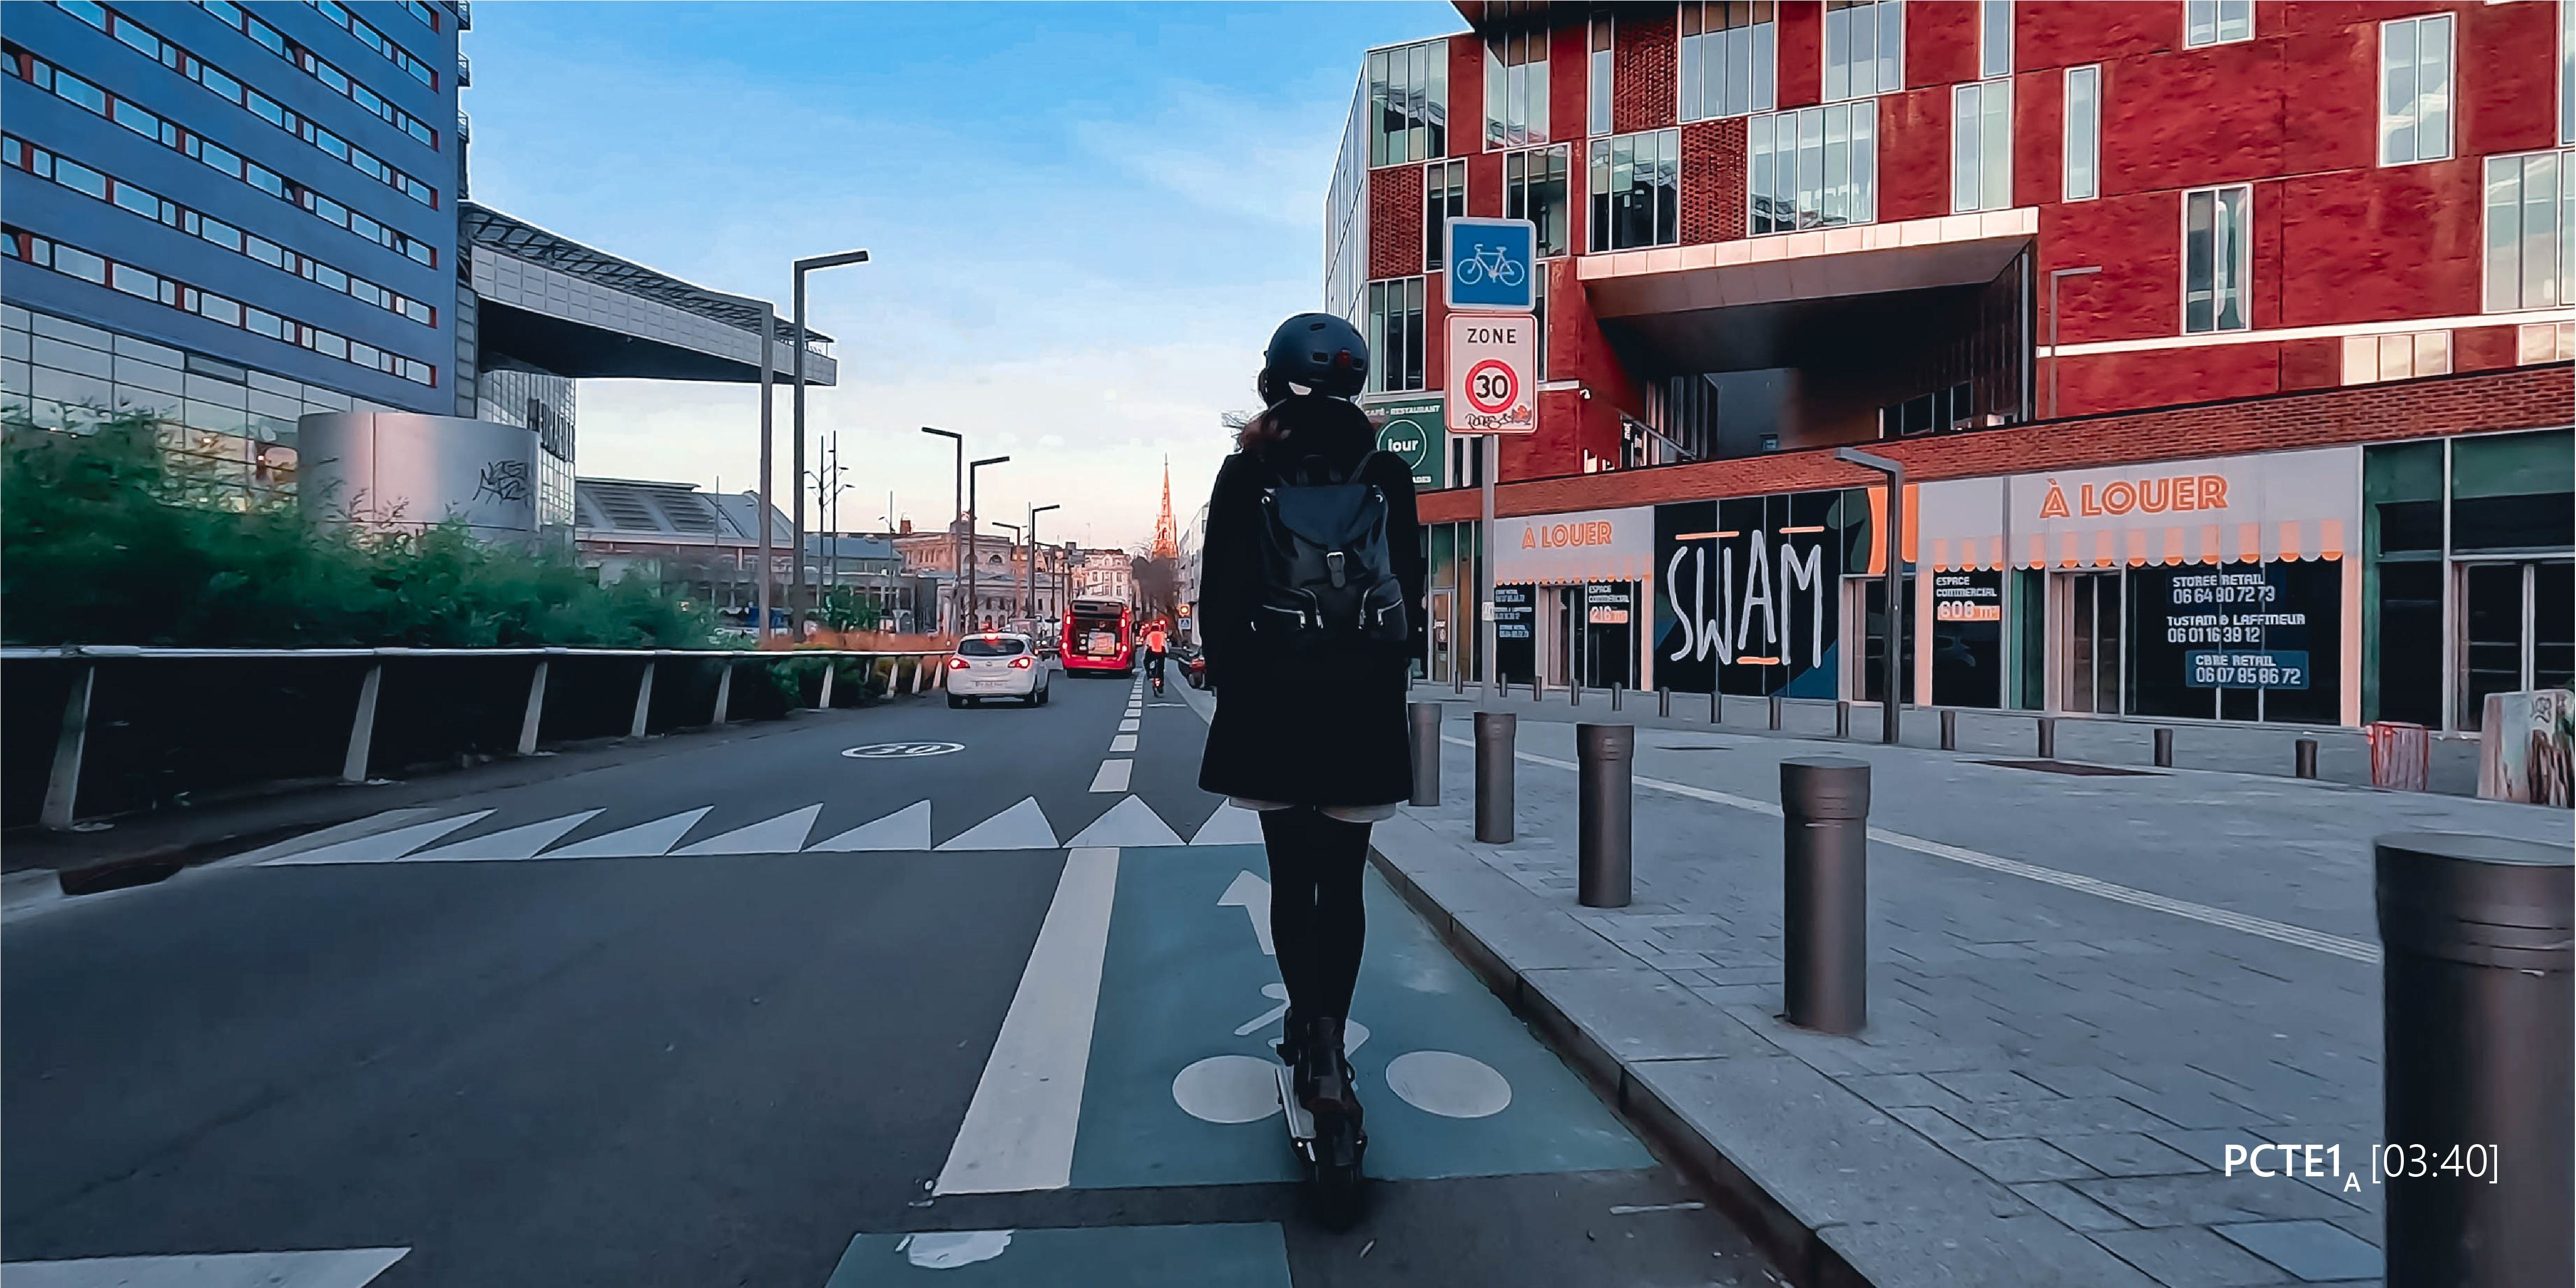
\includegraphics[width=0.75\columnwidth]{src/Figures/Annexes/Extrait_Video_PCTE1_Access_10.jpg}}
        \vspace{5pt}
        \begin{flushright}\scriptsize{
        Auteur~: \textcolor{blue}{Dylan Moinse (2022)}
        }\end{flushright}
    \end{figure}
    
    % PCTE1 Photo Access 11
    \begin{figure}[h!]\vspace*{4pt}
        \caption*{Extrait n°11 de la vidéo lors du trajet en rabattement (\(PCTE^{A}_{1}\))}
        \centerline{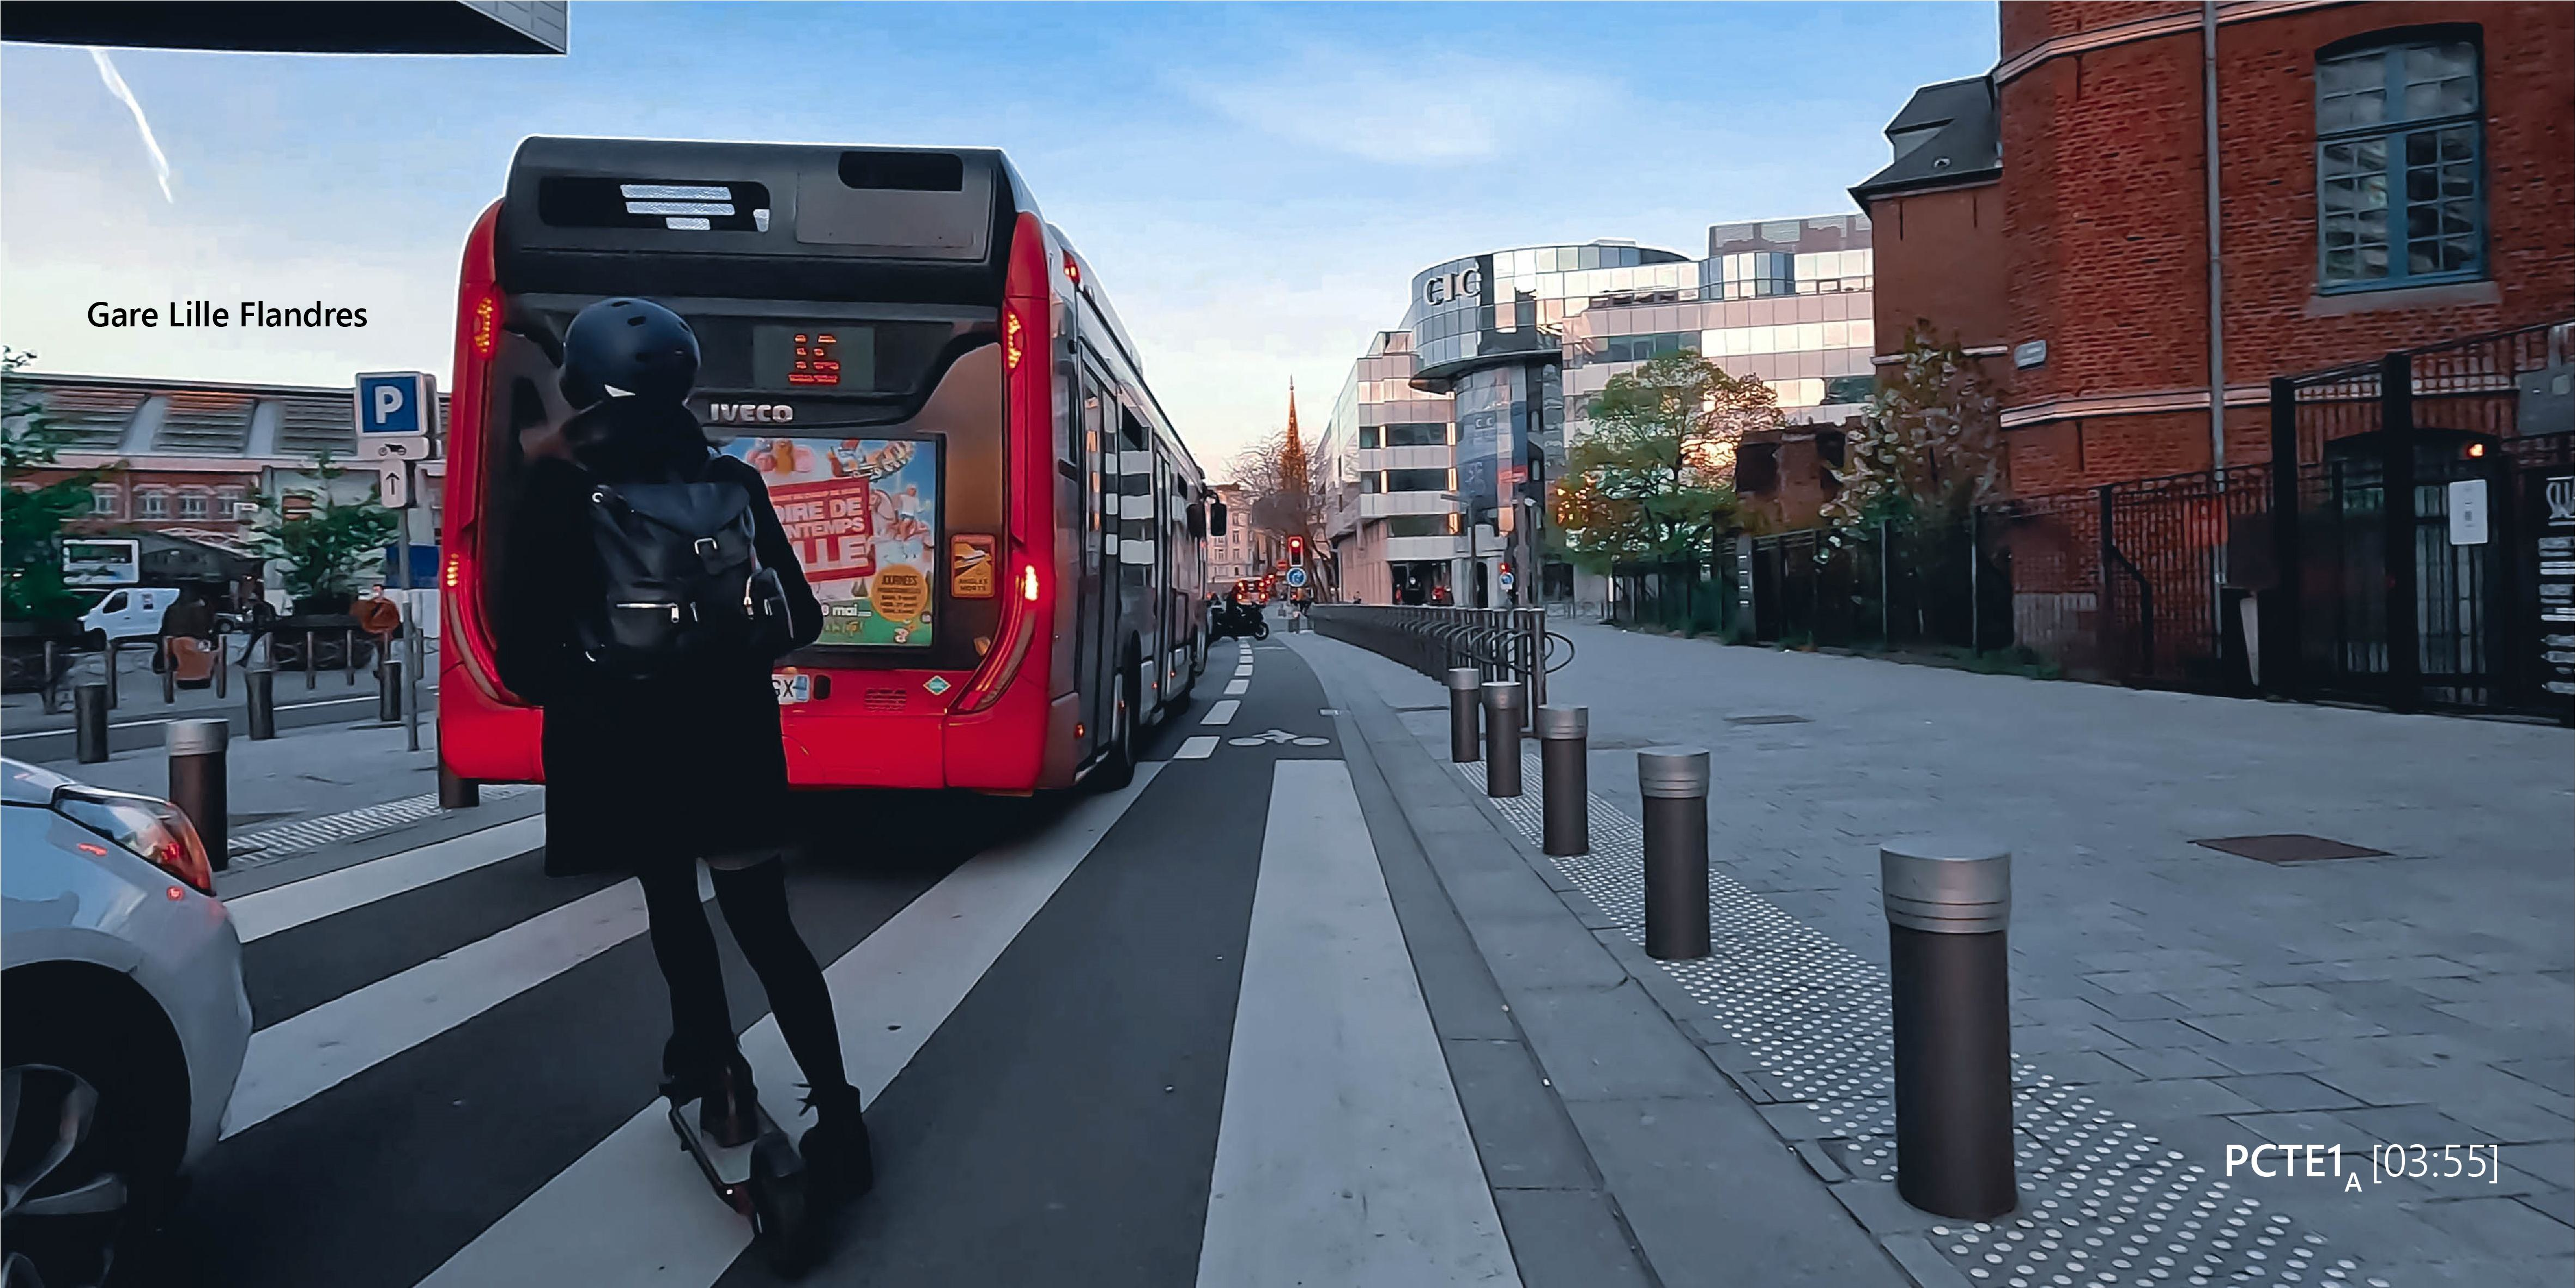
\includegraphics[width=0.75\columnwidth]{src/Figures/Annexes/Extrait_Video_PCTE1_Access_11.jpg}}
        \vspace{5pt}
        \begin{flushright}\scriptsize{
        Auteur~: \textcolor{blue}{Dylan Moinse (2022)}
        }\end{flushright}
    \end{figure}

    % PCTE1 Photo Access 12
    \begin{figure}[h!]\vspace*{4pt}
        \caption*{Extrait n°12 de la vidéo lors du trajet en rabattement (\(PCTE^{A}_{1}\))}
        \centerline{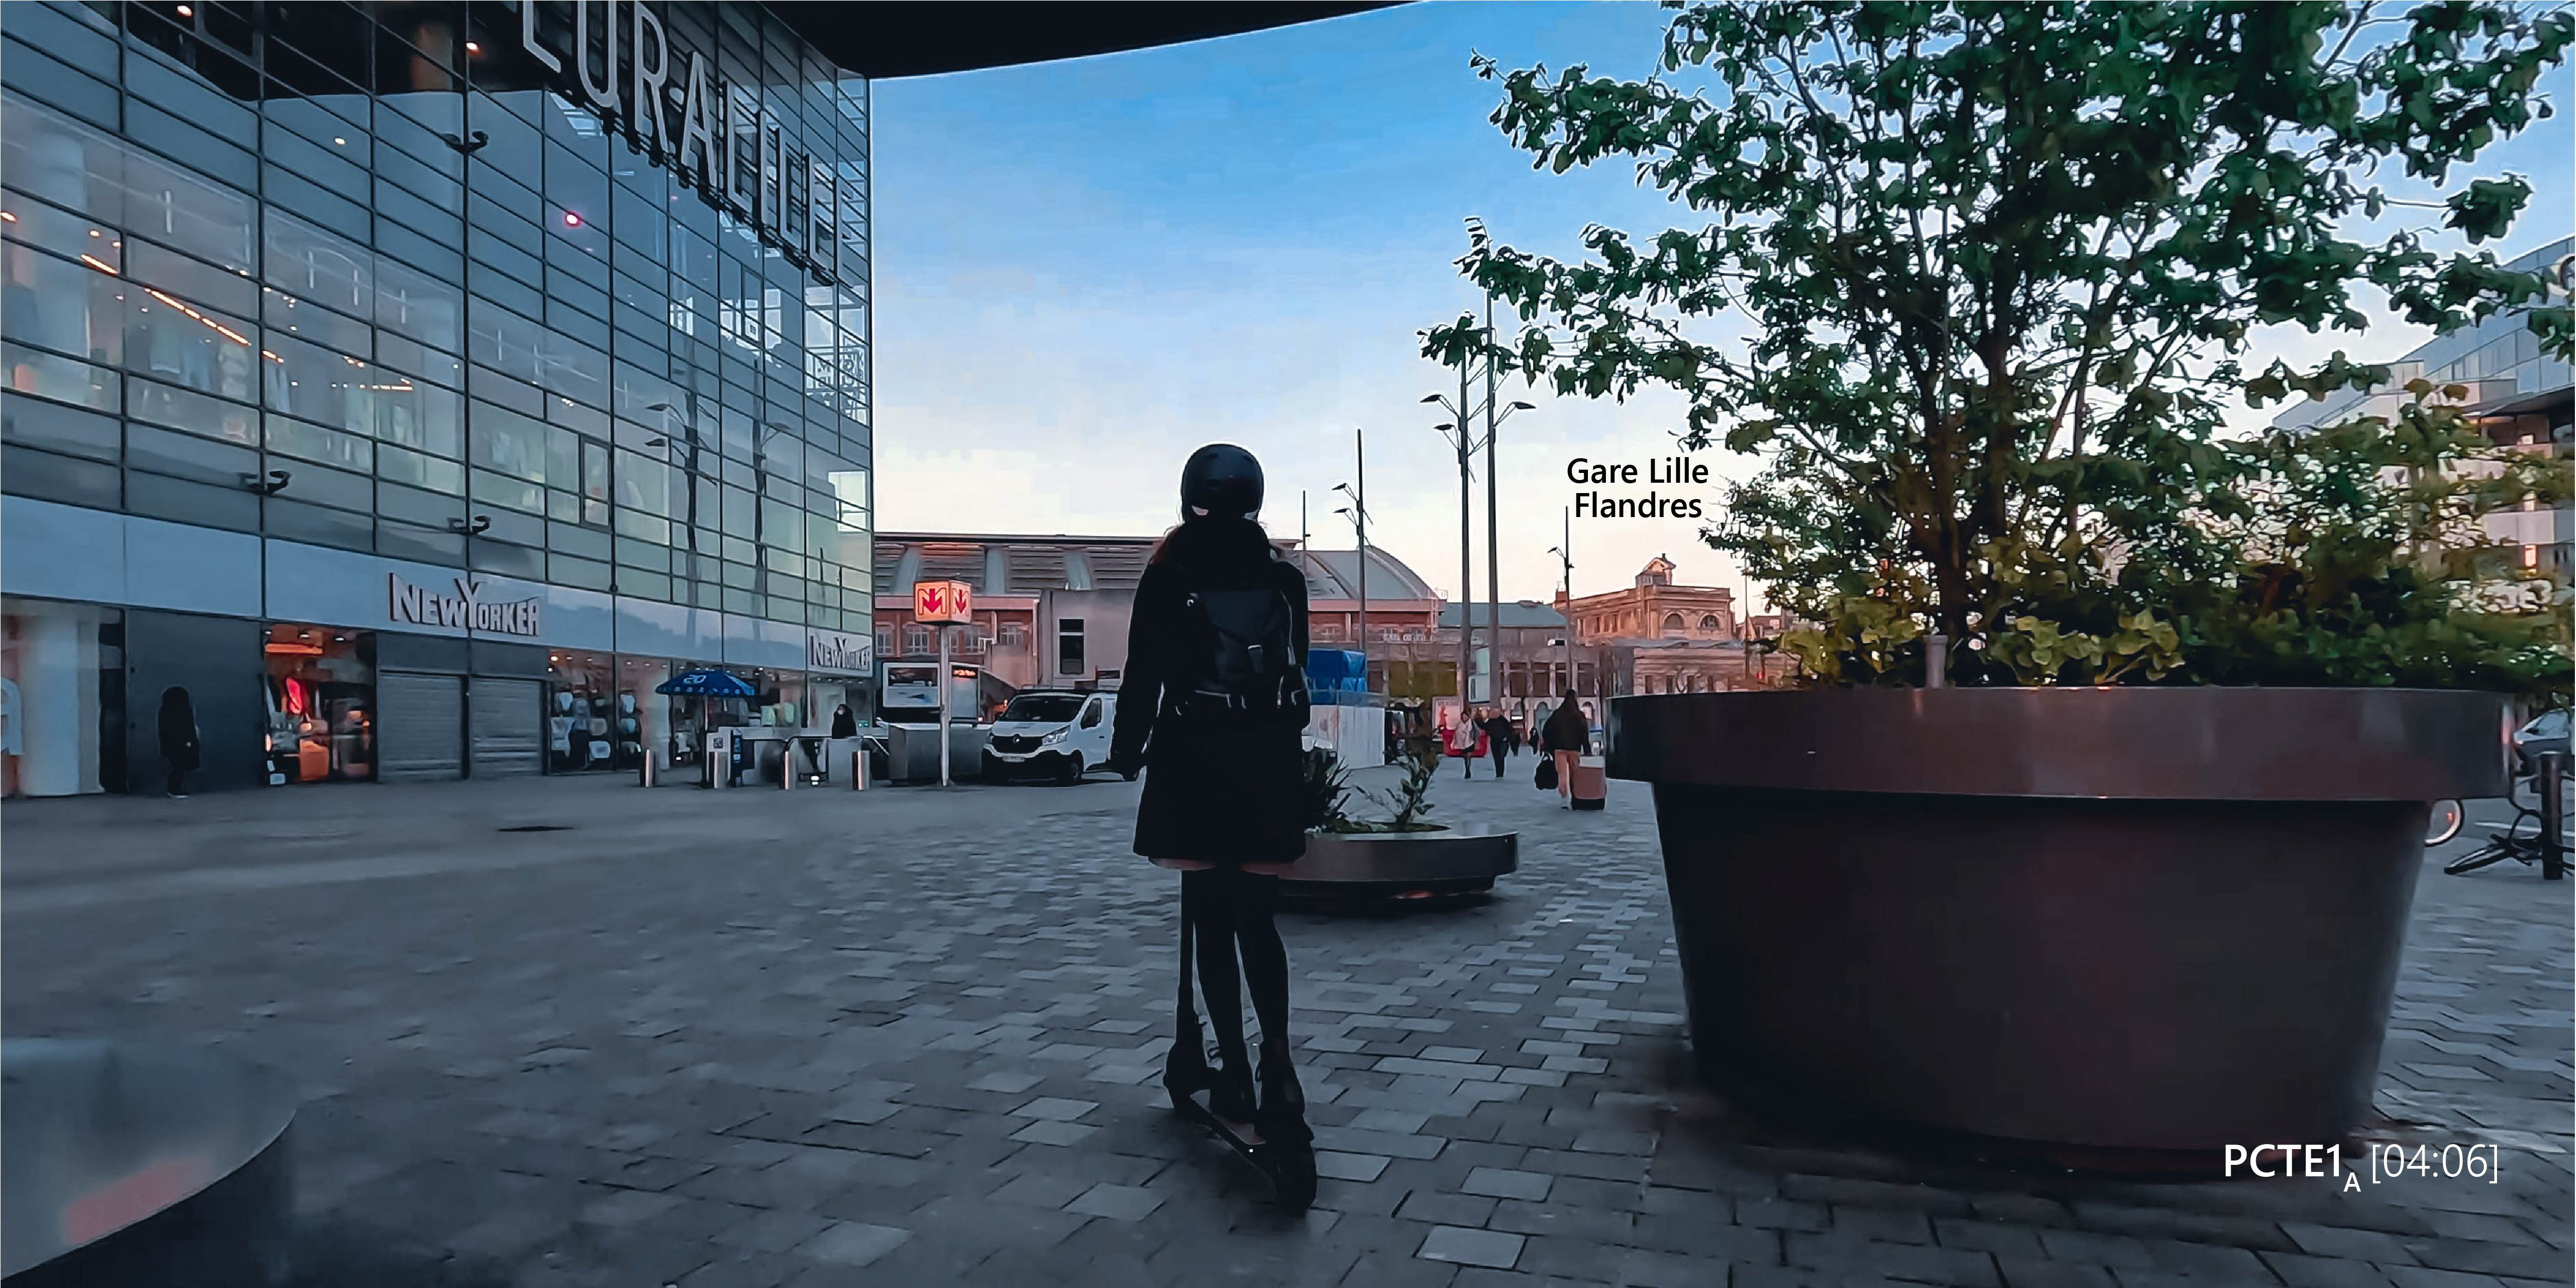
\includegraphics[width=0.75\columnwidth]{src/Figures/Annexes/Extrait_Video_PCTE1_Access_12.jpg}}
        \vspace{5pt}
        \begin{flushright}\scriptsize{
        Auteur~: \textcolor{blue}{Dylan Moinse (2022)}
        }\end{flushright}
    \end{figure}

    % PCTE1 Photo Access 13
    \begin{figure}[h!]\vspace*{4pt}
        \caption*{Extrait n°13 de la vidéo lors du trajet en rabattement (\(PCTE^{A}_{1}\))}
        \centerline{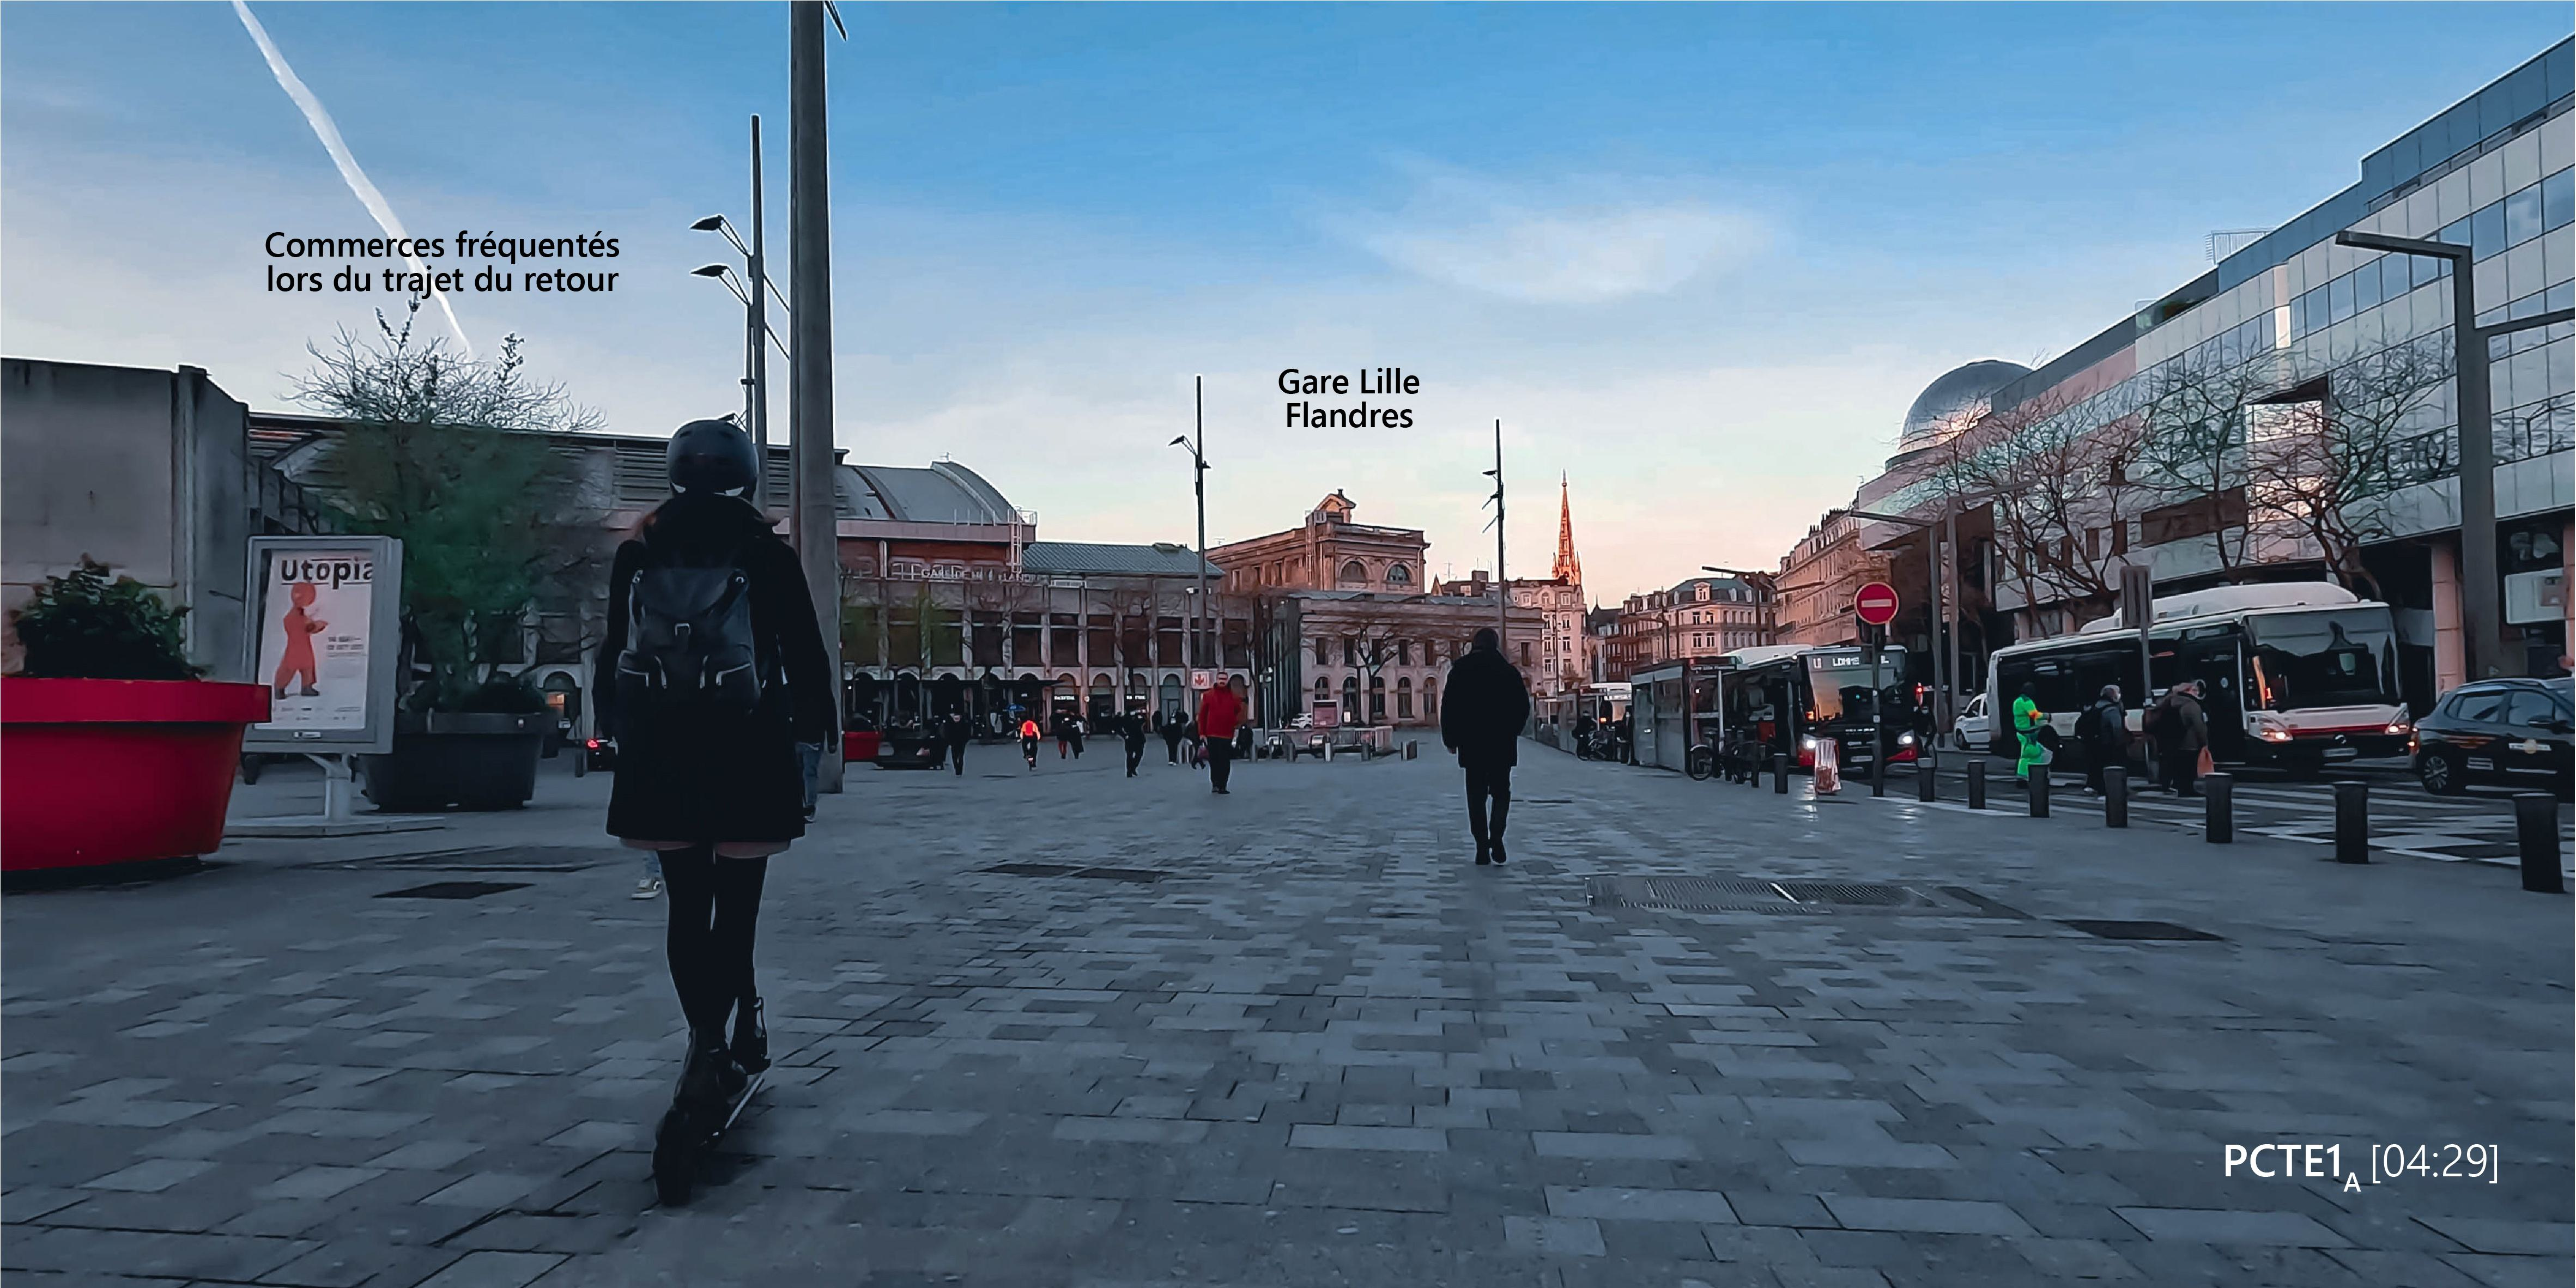
\includegraphics[width=0.75\columnwidth]{src/Figures/Annexes/Extrait_Video_PCTE1_Access_13.jpg}}
        \vspace{5pt}
        \begin{flushright}\scriptsize{
        Auteur~: \textcolor{blue}{Dylan Moinse (2022)}
        }\end{flushright}
    \end{figure}


    % Photos PCTE1 TC
\subsubsection{Sélection d'images extraites lors du trajet en train}

    % PCTE1 Photo TC 1
    \begin{figure}[h!]\vspace*{4pt}
        \caption*{Extrait n°1 de la vidéo lors du trajet en TER (\(PCTE^{TC}_{1}\))}
        \centerline{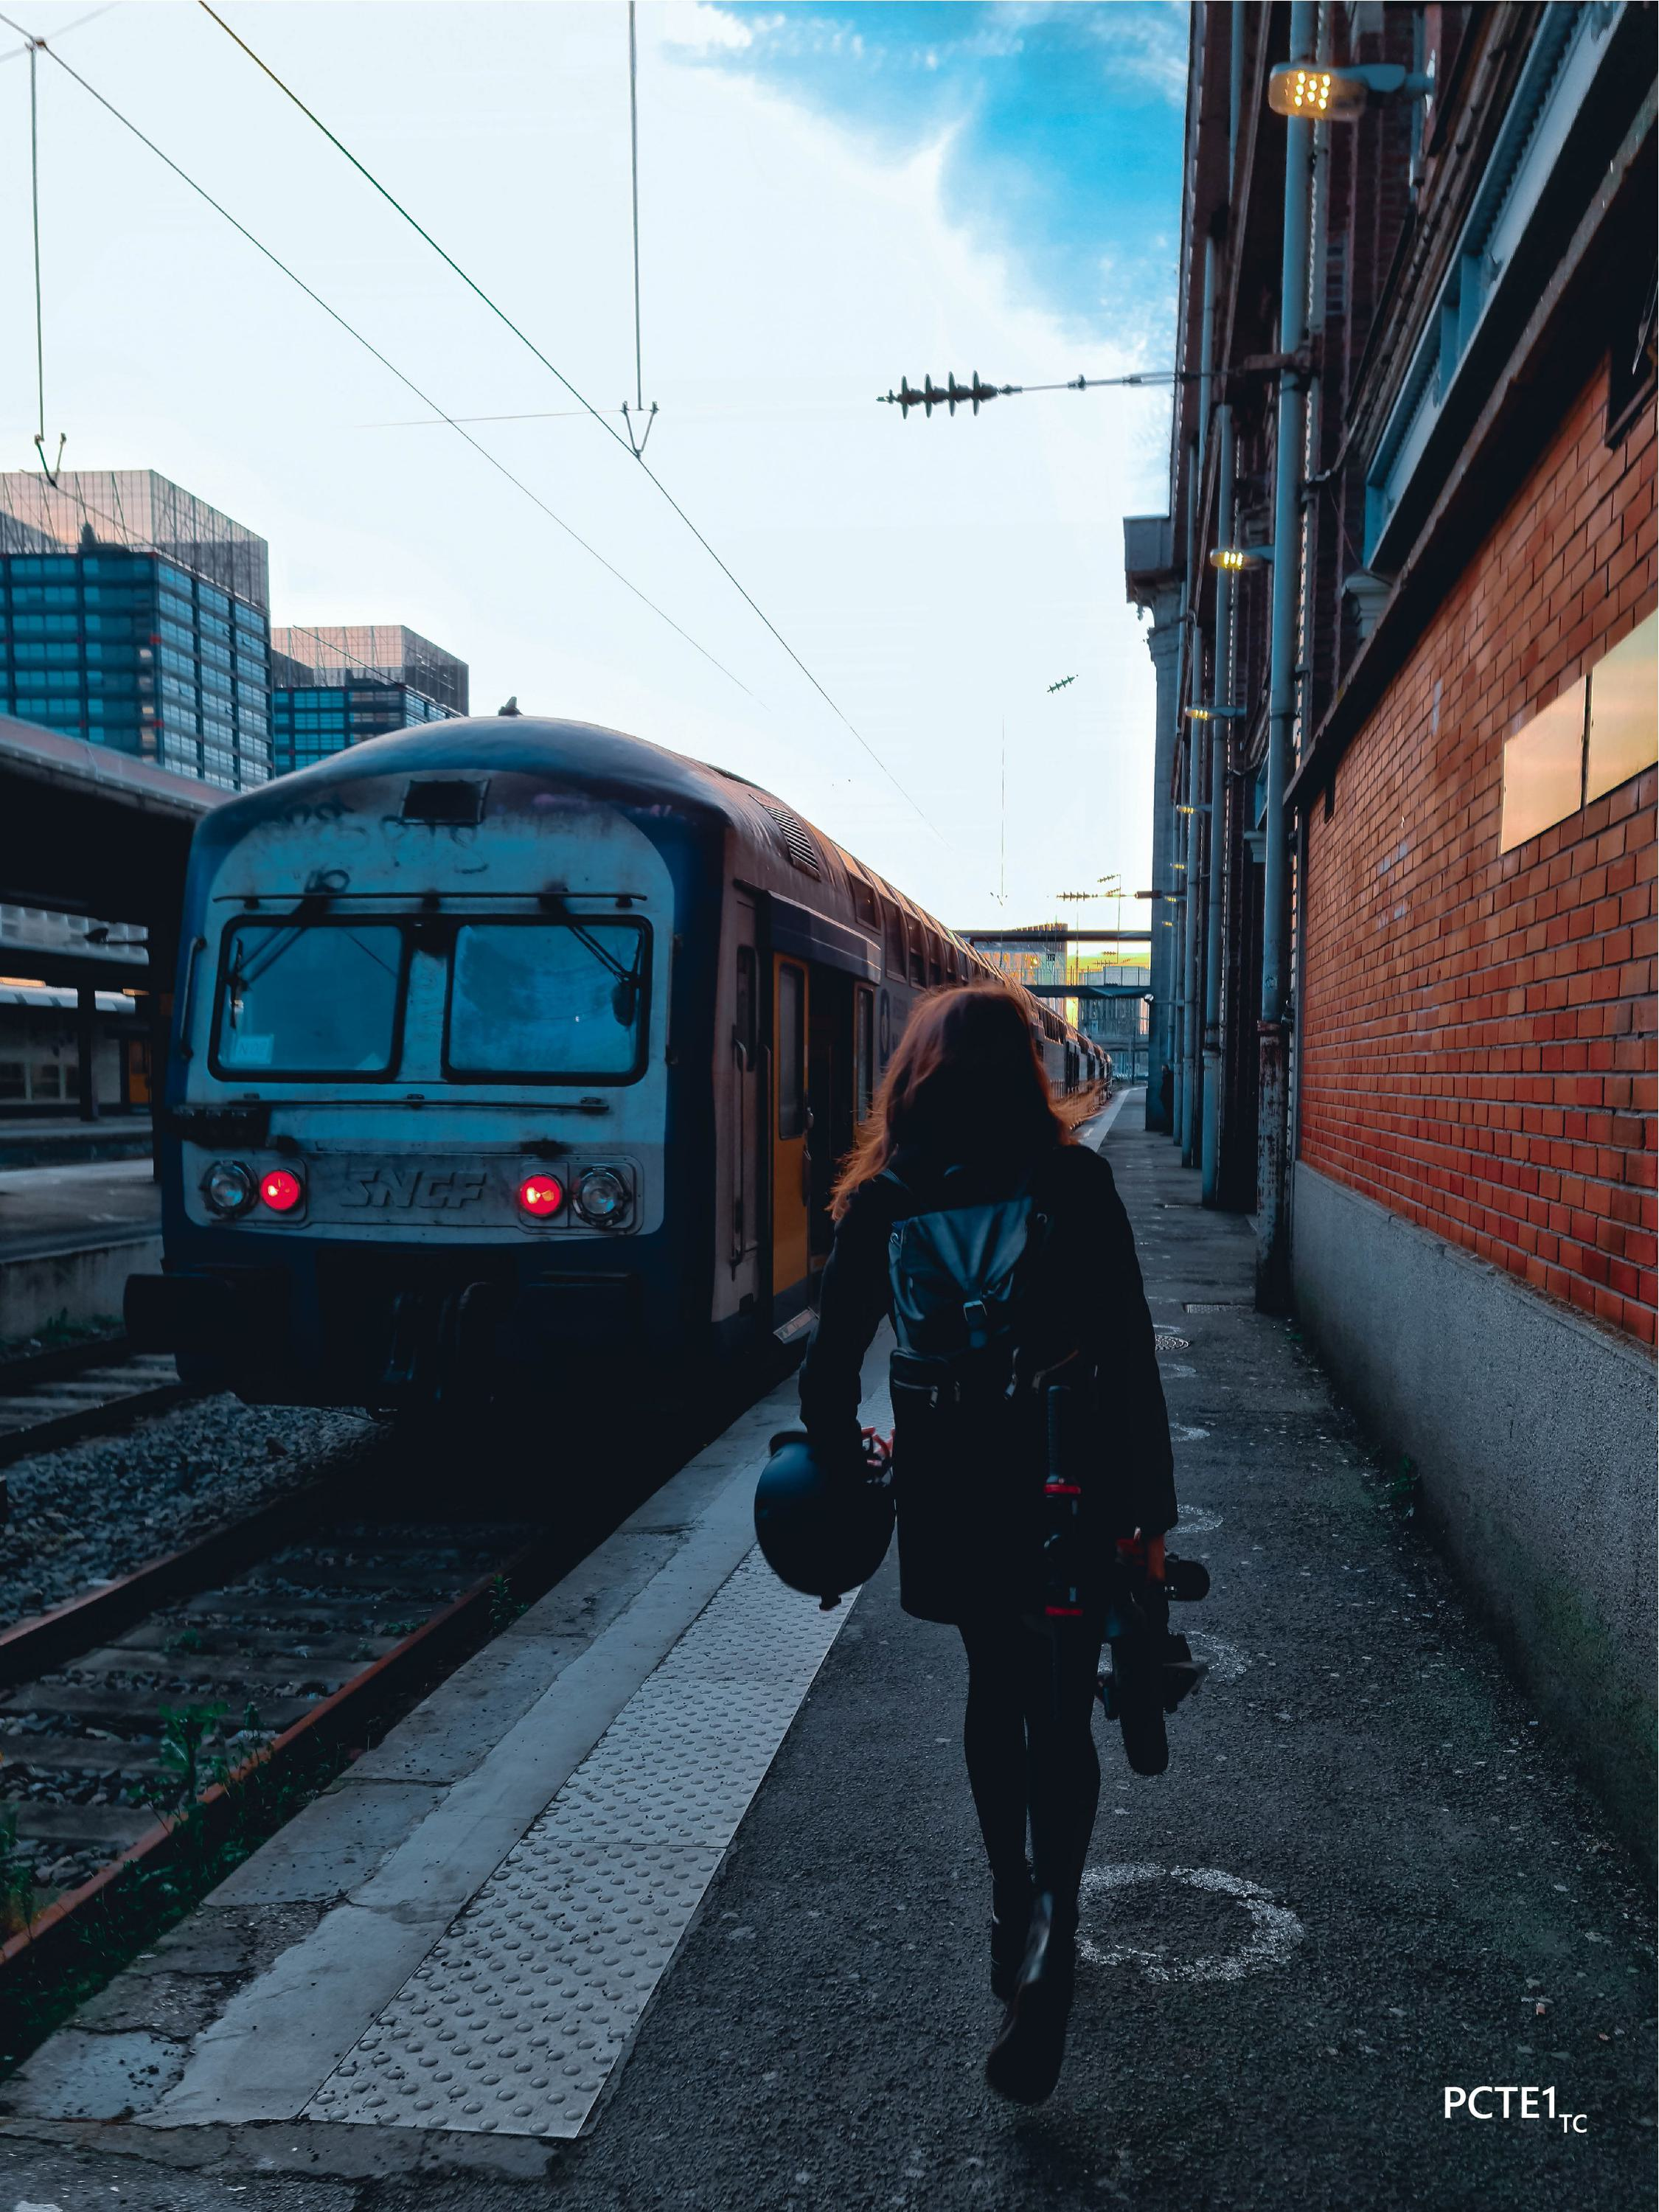
\includegraphics[width=0.5\columnwidth]{src/Figures/Annexes/Extrait_Video_PCTE1_TC_1.jpg}}
        \vspace{5pt}
        \begin{flushright}\scriptsize{
        Auteur~: \textcolor{blue}{Dylan Moinse (2022)}
        }\end{flushright}
    \end{figure}

    % PCTE1 Photo TC 2
    \begin{figure}[h!]\vspace*{4pt}
        \caption*{Extrait n°2 de la vidéo lors du trajet en TER (\(PCTE^{TC}_{1}\))}
        \centerline{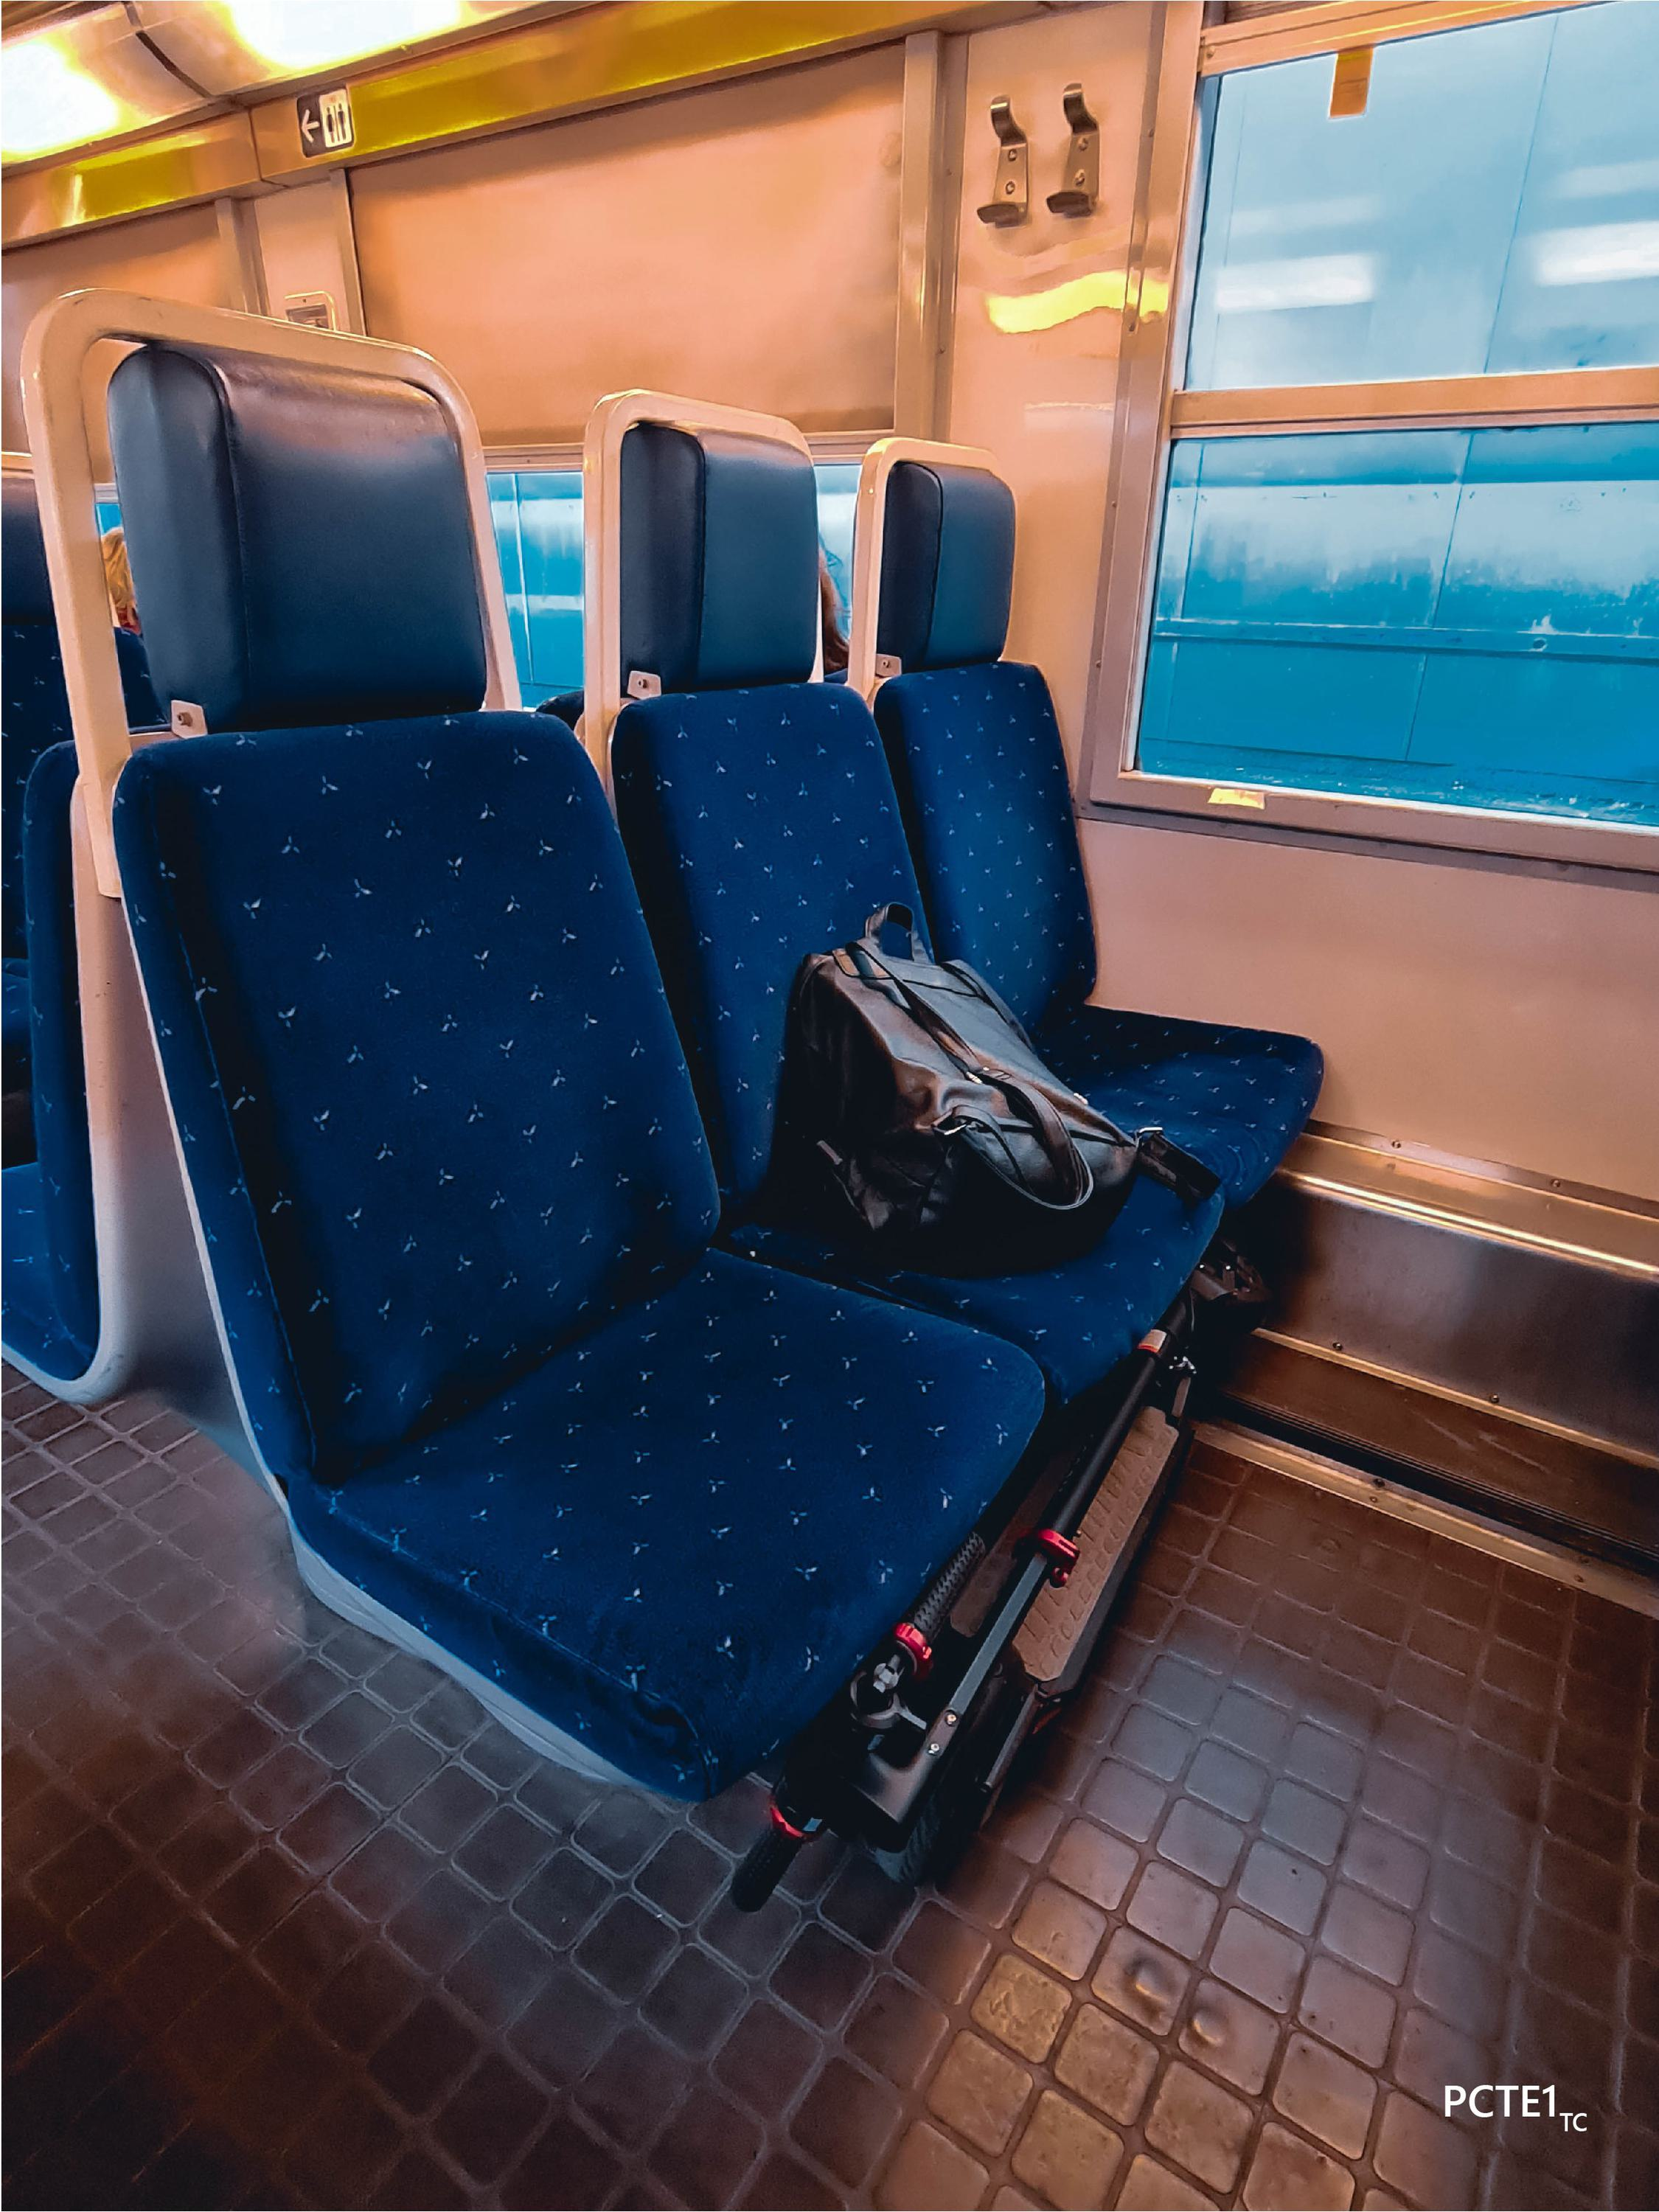
\includegraphics[width=0.5\columnwidth]{src/Figures/Annexes/Extrait_Video_PCTE1_TC_2.jpg}}
        \vspace{5pt}
        \begin{flushright}\scriptsize{
        Auteur~: \textcolor{blue}{Dylan Moinse (2022)}
        }\end{flushright}
    \end{figure}

    % PCTE1 Photo TC 3
    \begin{figure}[h!]\vspace*{4pt}
        \caption*{Extrait n°3 de la vidéo lors du trajet en TER (\(PCTE^{TC}_{1}\))}
        \centerline{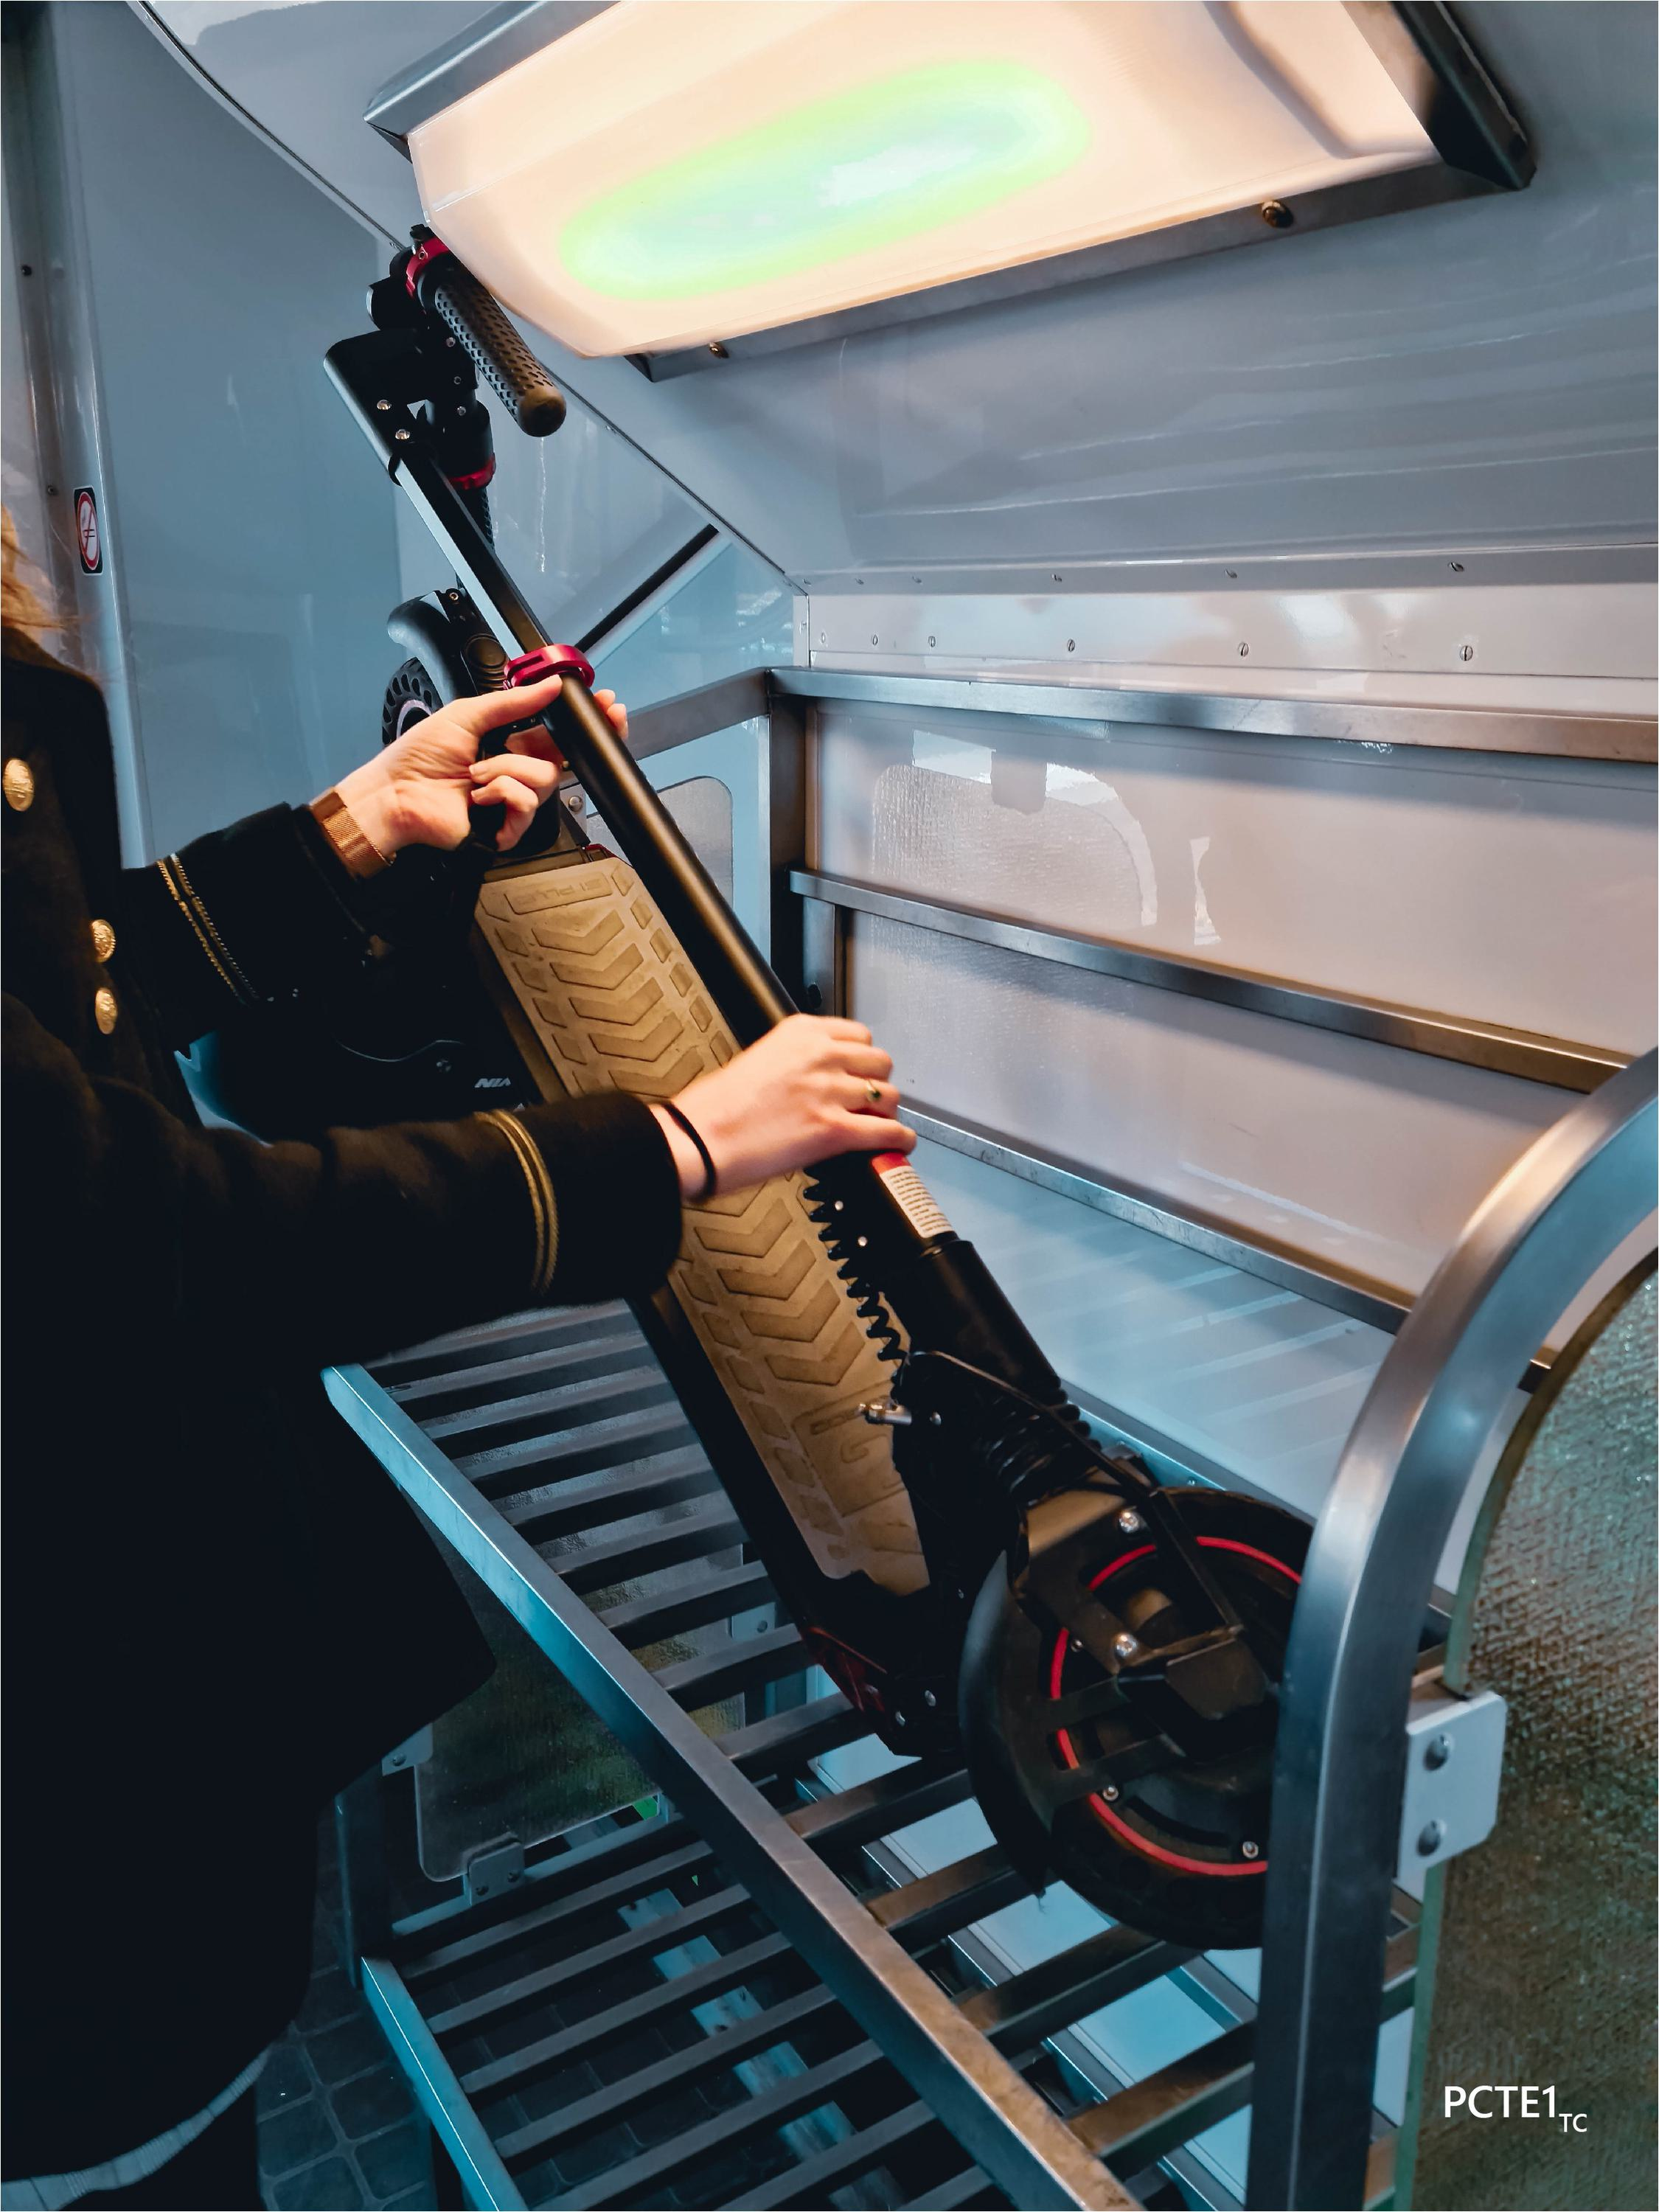
\includegraphics[width=0.5\columnwidth]{src/Figures/Annexes/Extrait_Video_PCTE1_TC_3.jpg}}
        \vspace{5pt}
        \begin{flushright}\scriptsize{
        Auteur~: \textcolor{blue}{Dylan Moinse (2022)}
        }\end{flushright}
    \end{figure}

    % Photos PCTE1 egress
\subsubsection{Sélection d'images extraites lors du trajet en diffusion}

    % PCTE1 Photo Egress 1
    \begin{figure}[h!]\vspace*{4pt}
        \caption*{Extrait n°1 de la vidéo lors du trajet en diffusion (\(PCTE^{E}_{1}\))}
        \centerline{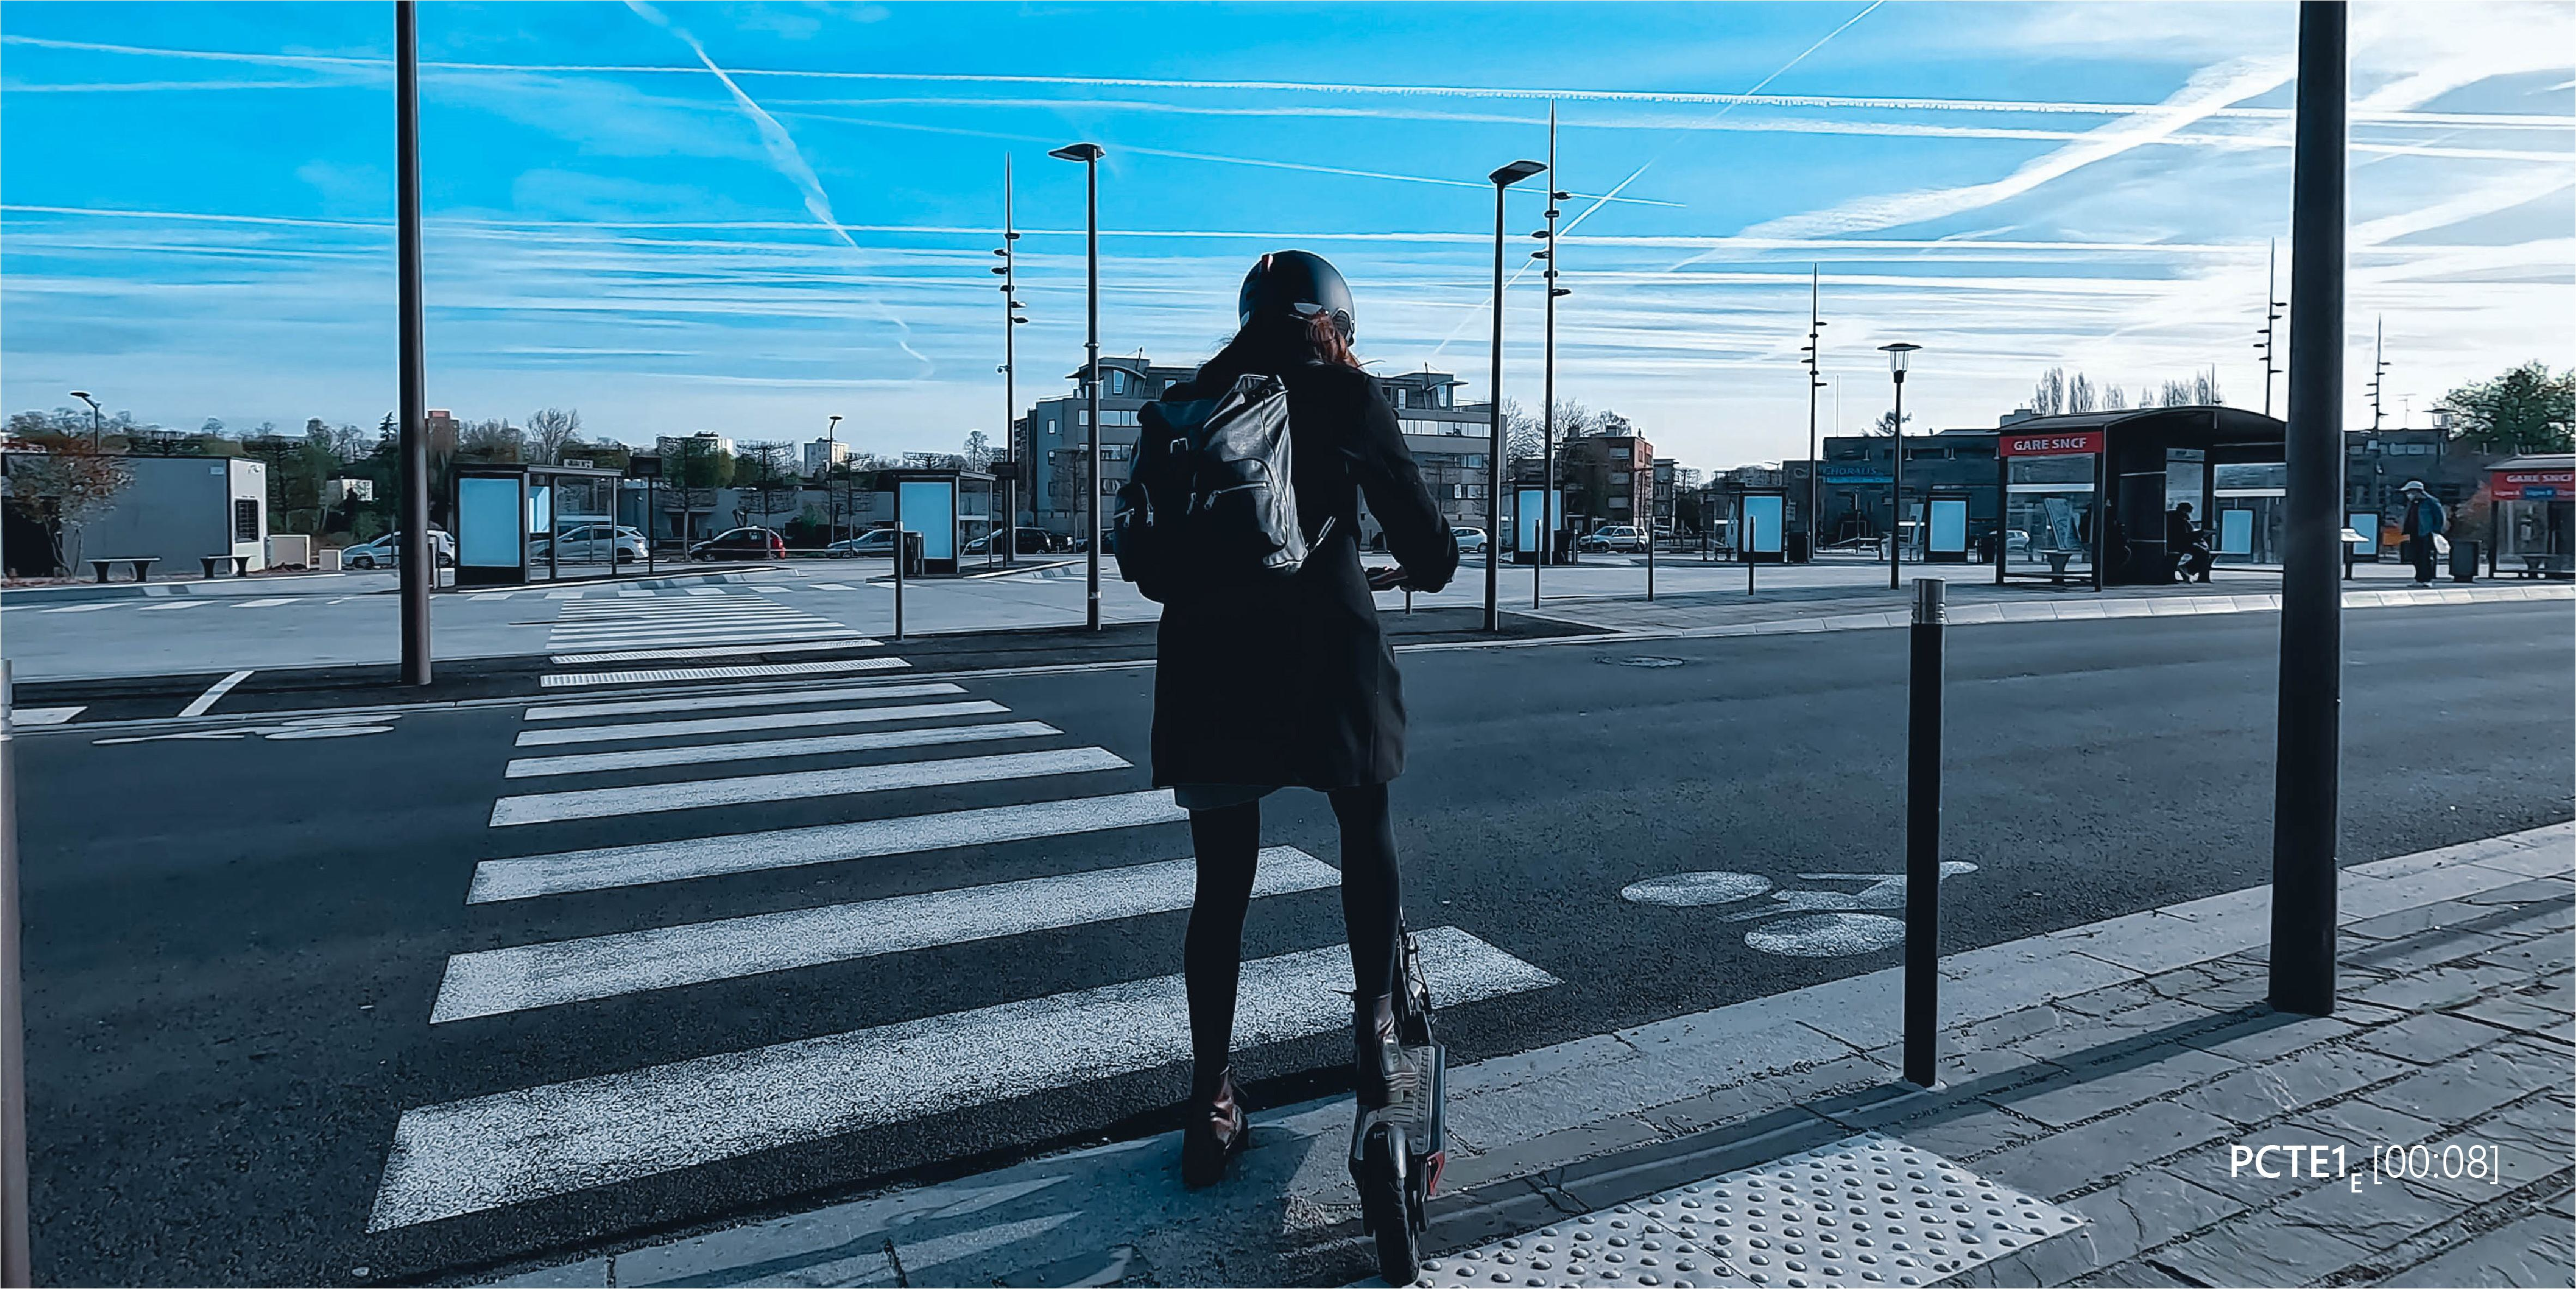
\includegraphics[width=0.75\columnwidth]{src/Figures/Annexes/Extrait_Video_PCTE1_Egress_1.jpg}}
        \vspace{5pt}
        \begin{flushright}\scriptsize{
        Auteur~: \textcolor{blue}{Dylan Moinse (2022)}
        }\end{flushright}
    \end{figure}

    % PCTE1 Photo Egress 2
    \begin{figure}[h!]\vspace*{4pt}
        \caption*{Extrait n°2 de la vidéo lors du trajet en diffusion (\(PCTE^{E}_{1}\))}
        \centerline{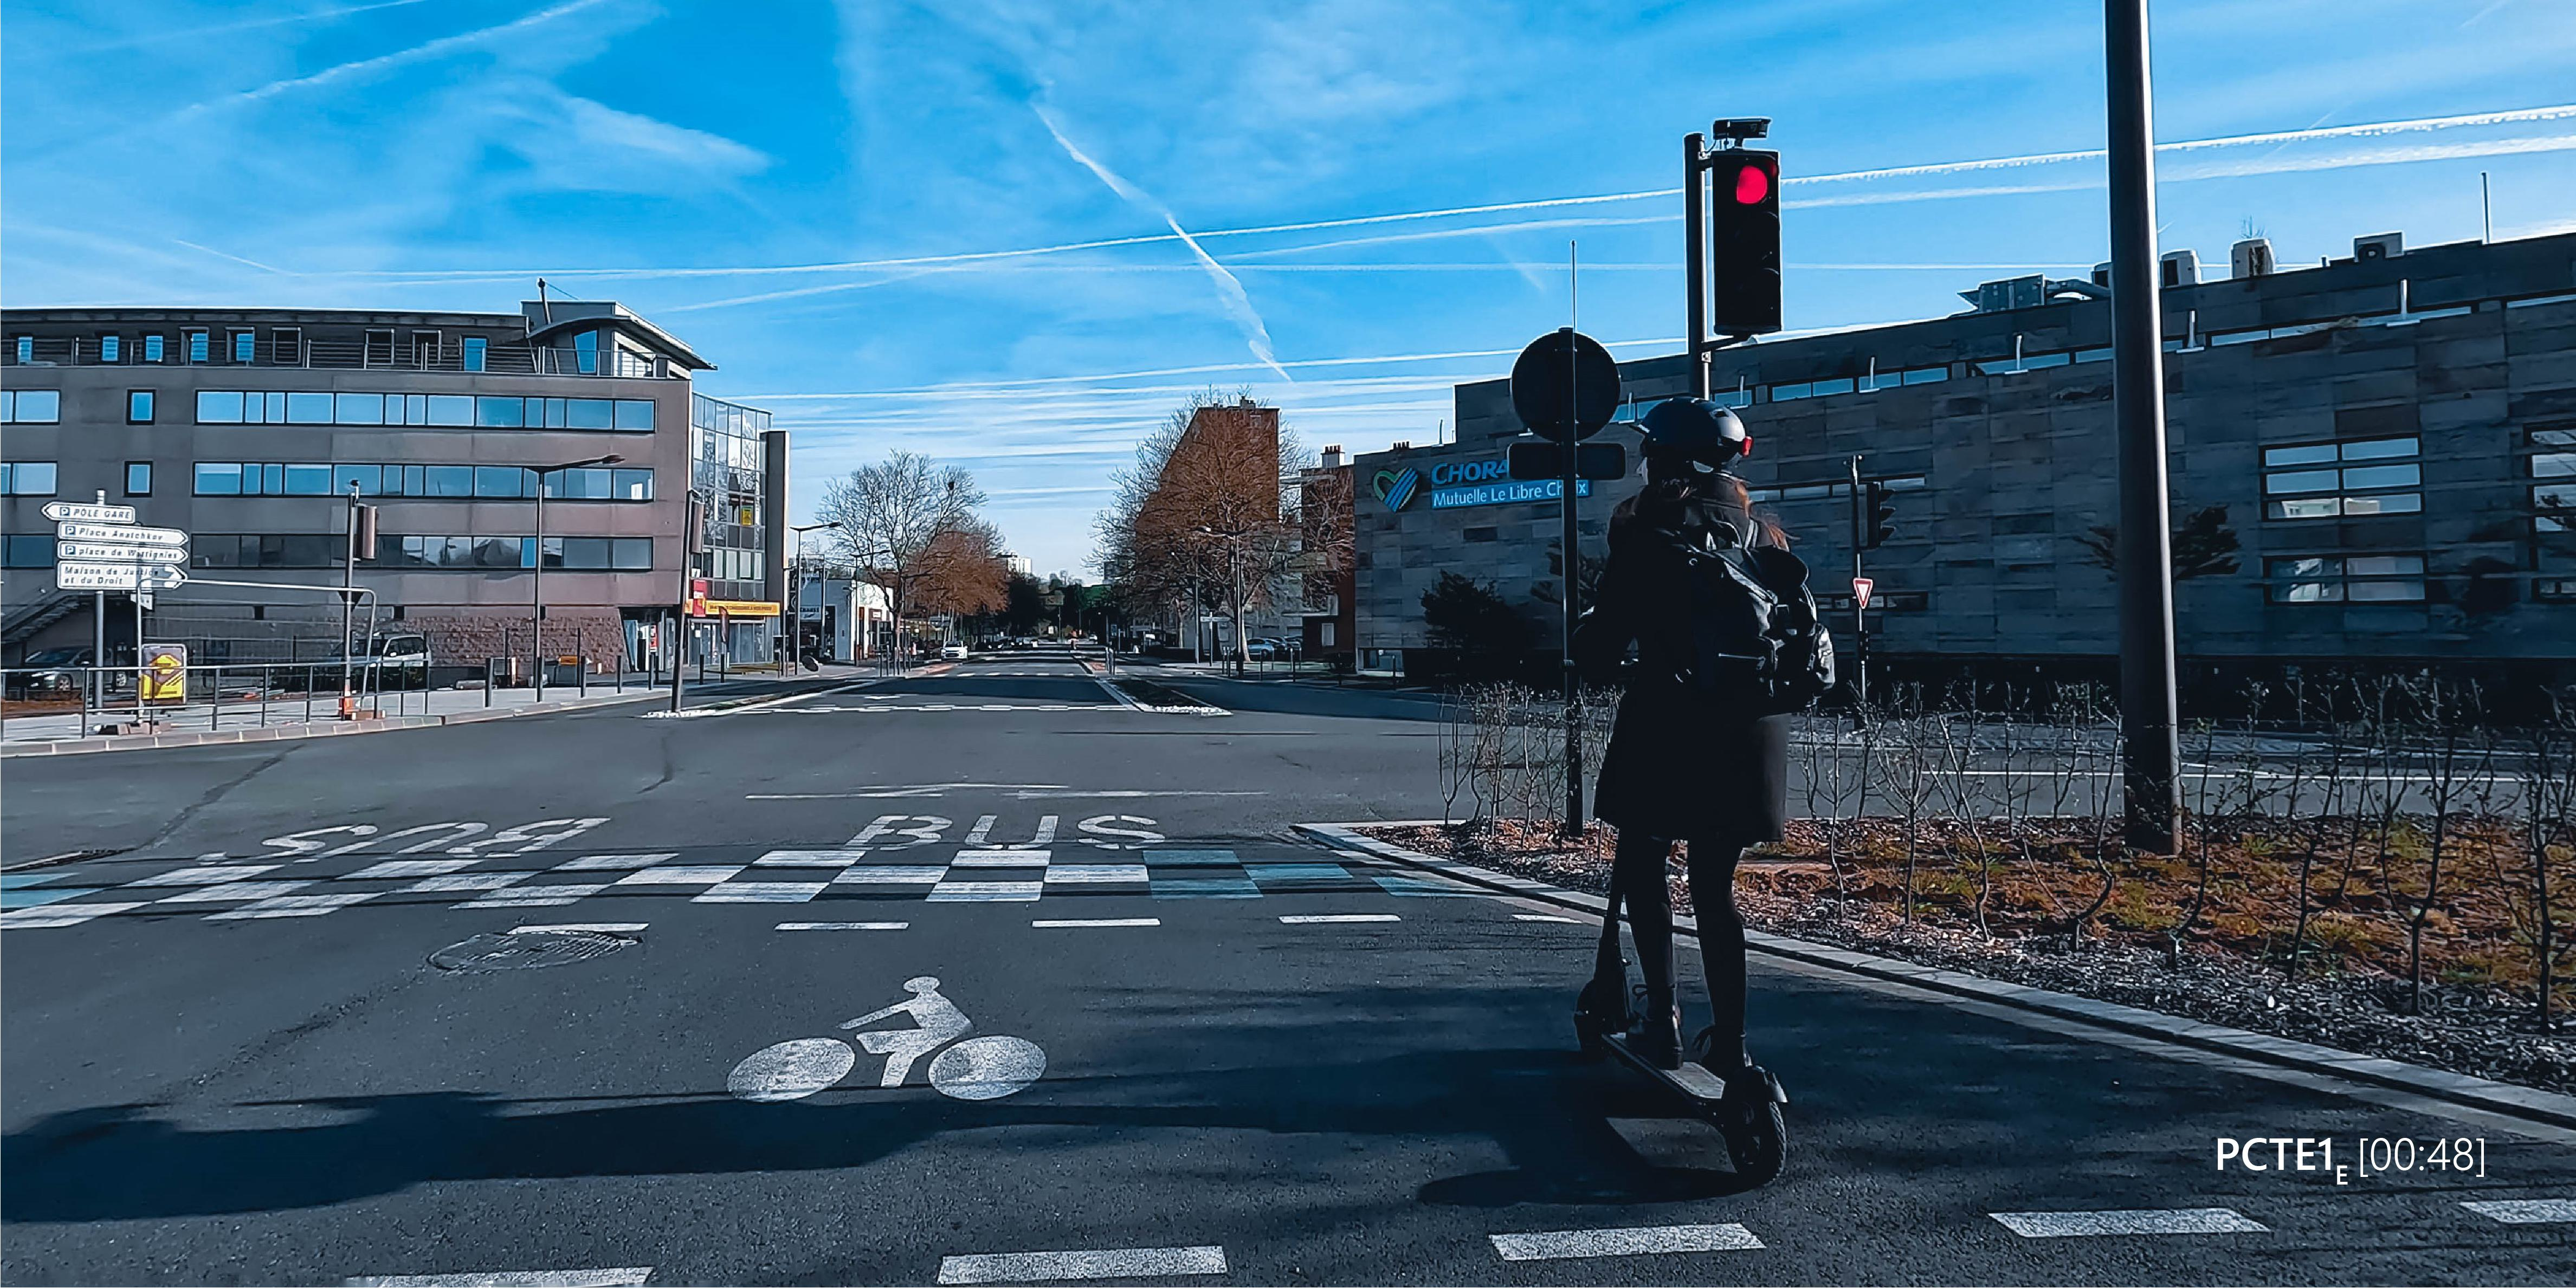
\includegraphics[width=0.75\columnwidth]{src/Figures/Annexes/Extrait_Video_PCTE1_Egress_2.jpg}}
        \vspace{5pt}
        \begin{flushright}\scriptsize{
        Auteur~: \textcolor{blue}{Dylan Moinse (2022)}
        }\end{flushright}
    \end{figure}

    % PCTE1 Photo Egress 3
    \begin{figure}[h!]\vspace*{4pt}
        \caption*{Extrait n°3 de la vidéo lors du trajet en diffusion (\(PCTE^{E}_{1}\))}
        \centerline{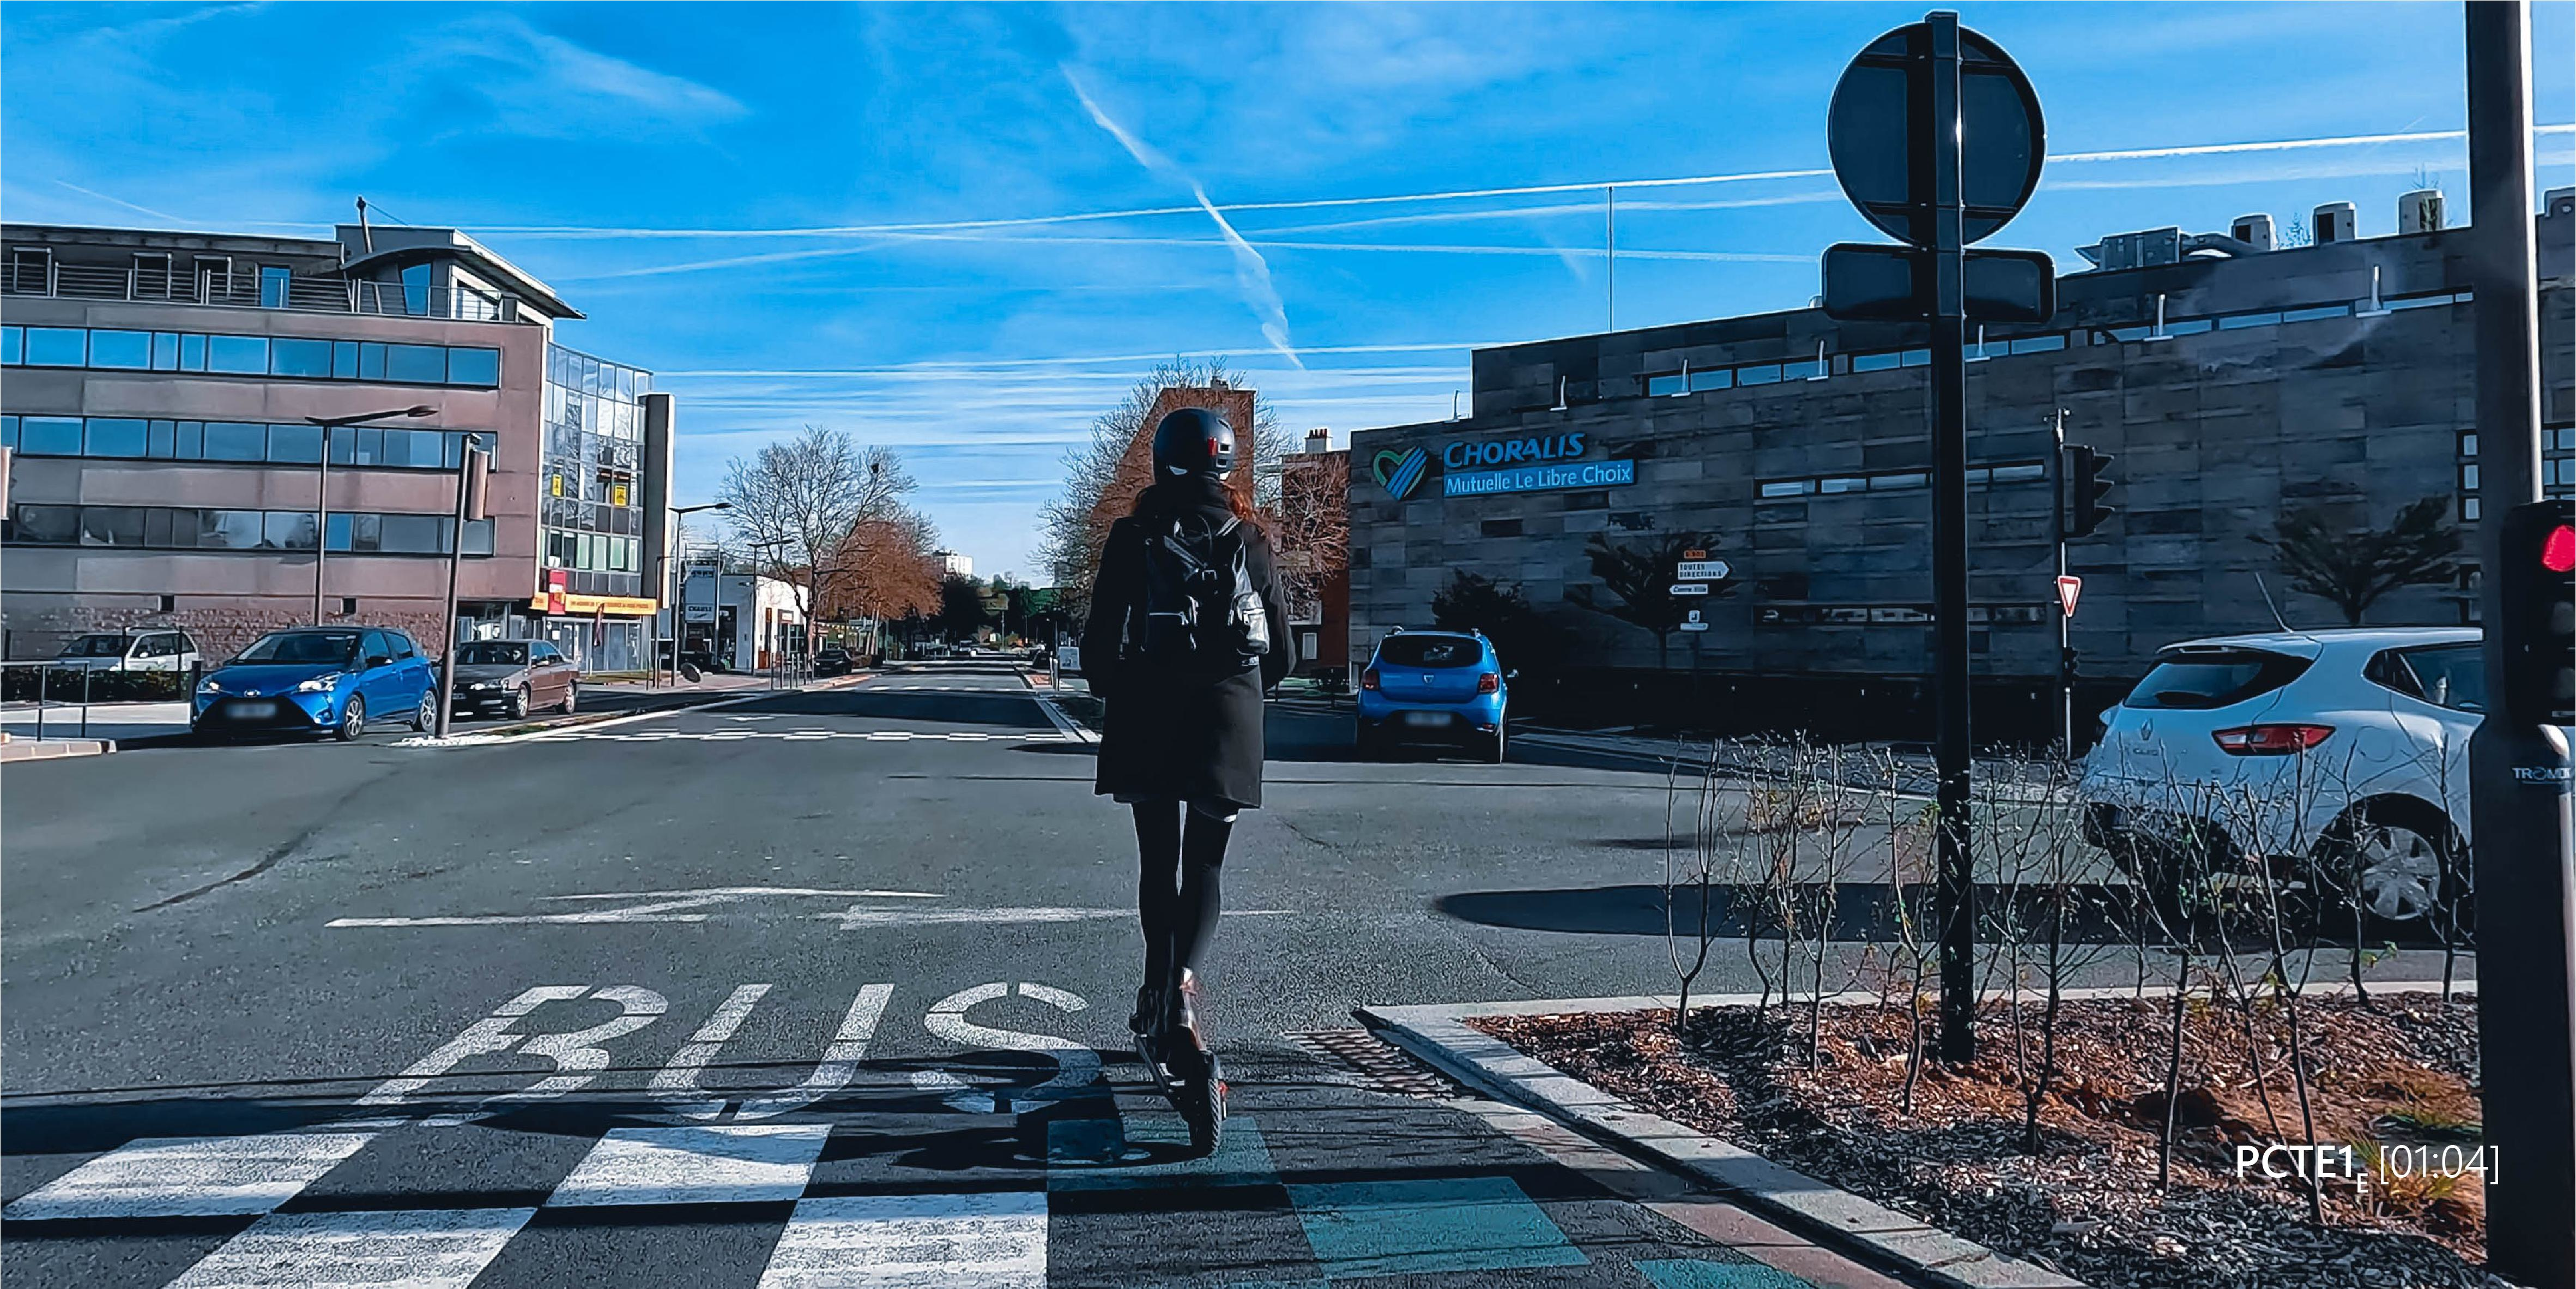
\includegraphics[width=0.75\columnwidth]{src/Figures/Annexes/Extrait_Video_PCTE1_Egress_3.jpg}}
        \vspace{5pt}
        \begin{flushright}\scriptsize{
        Auteur~: \textcolor{blue}{Dylan Moinse (2022)}
        }\end{flushright}
    \end{figure}

    % PCTE1 Photo Egress 4
    \begin{figure}[h!]\vspace*{4pt}
        \caption*{Extrait n°4 de la vidéo lors du trajet en diffusion (\(PCTE^{E}_{1}\))}
        \centerline{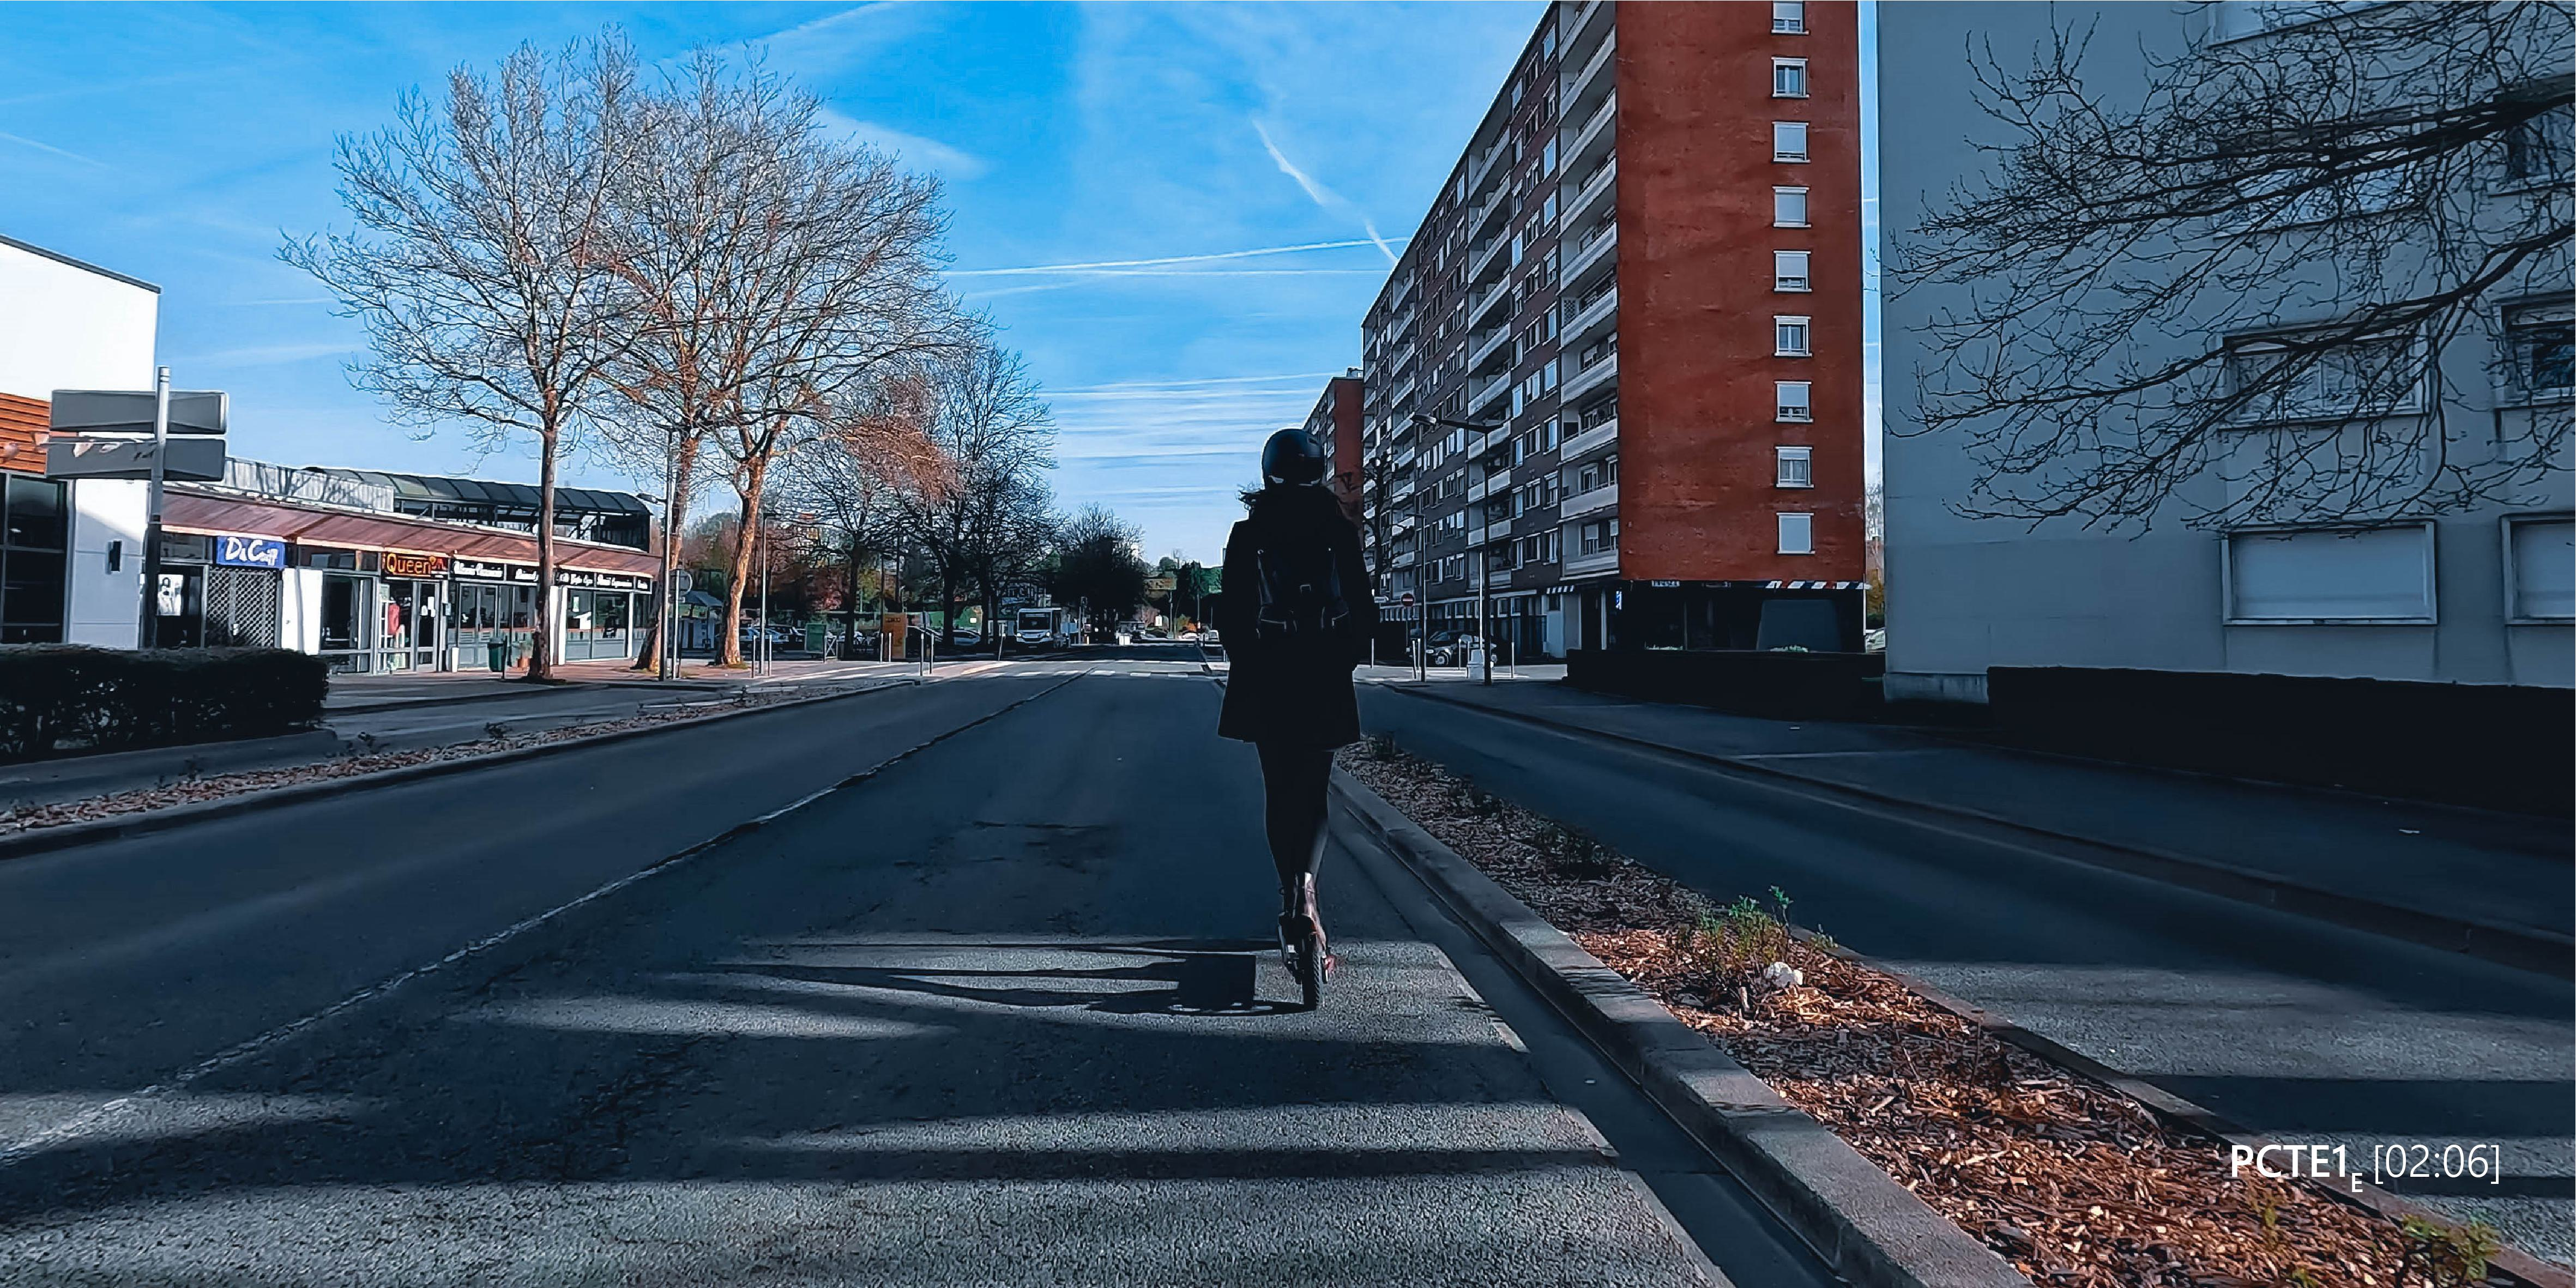
\includegraphics[width=0.75\columnwidth]{src/Figures/Annexes/Extrait_Video_PCTE1_Egress_4.jpg}}
        \vspace{5pt}
        \begin{flushright}\scriptsize{
        Auteur~: \textcolor{blue}{Dylan Moinse (2022)}
        }\end{flushright}
    \end{figure}

    % PCTE1 Photo Egress 5
    \begin{figure}[h!]\vspace*{4pt}
        \caption*{Extrait n°5 de la vidéo lors du trajet en diffusion (\(PCTE^{E}_{1}\))}
        \centerline{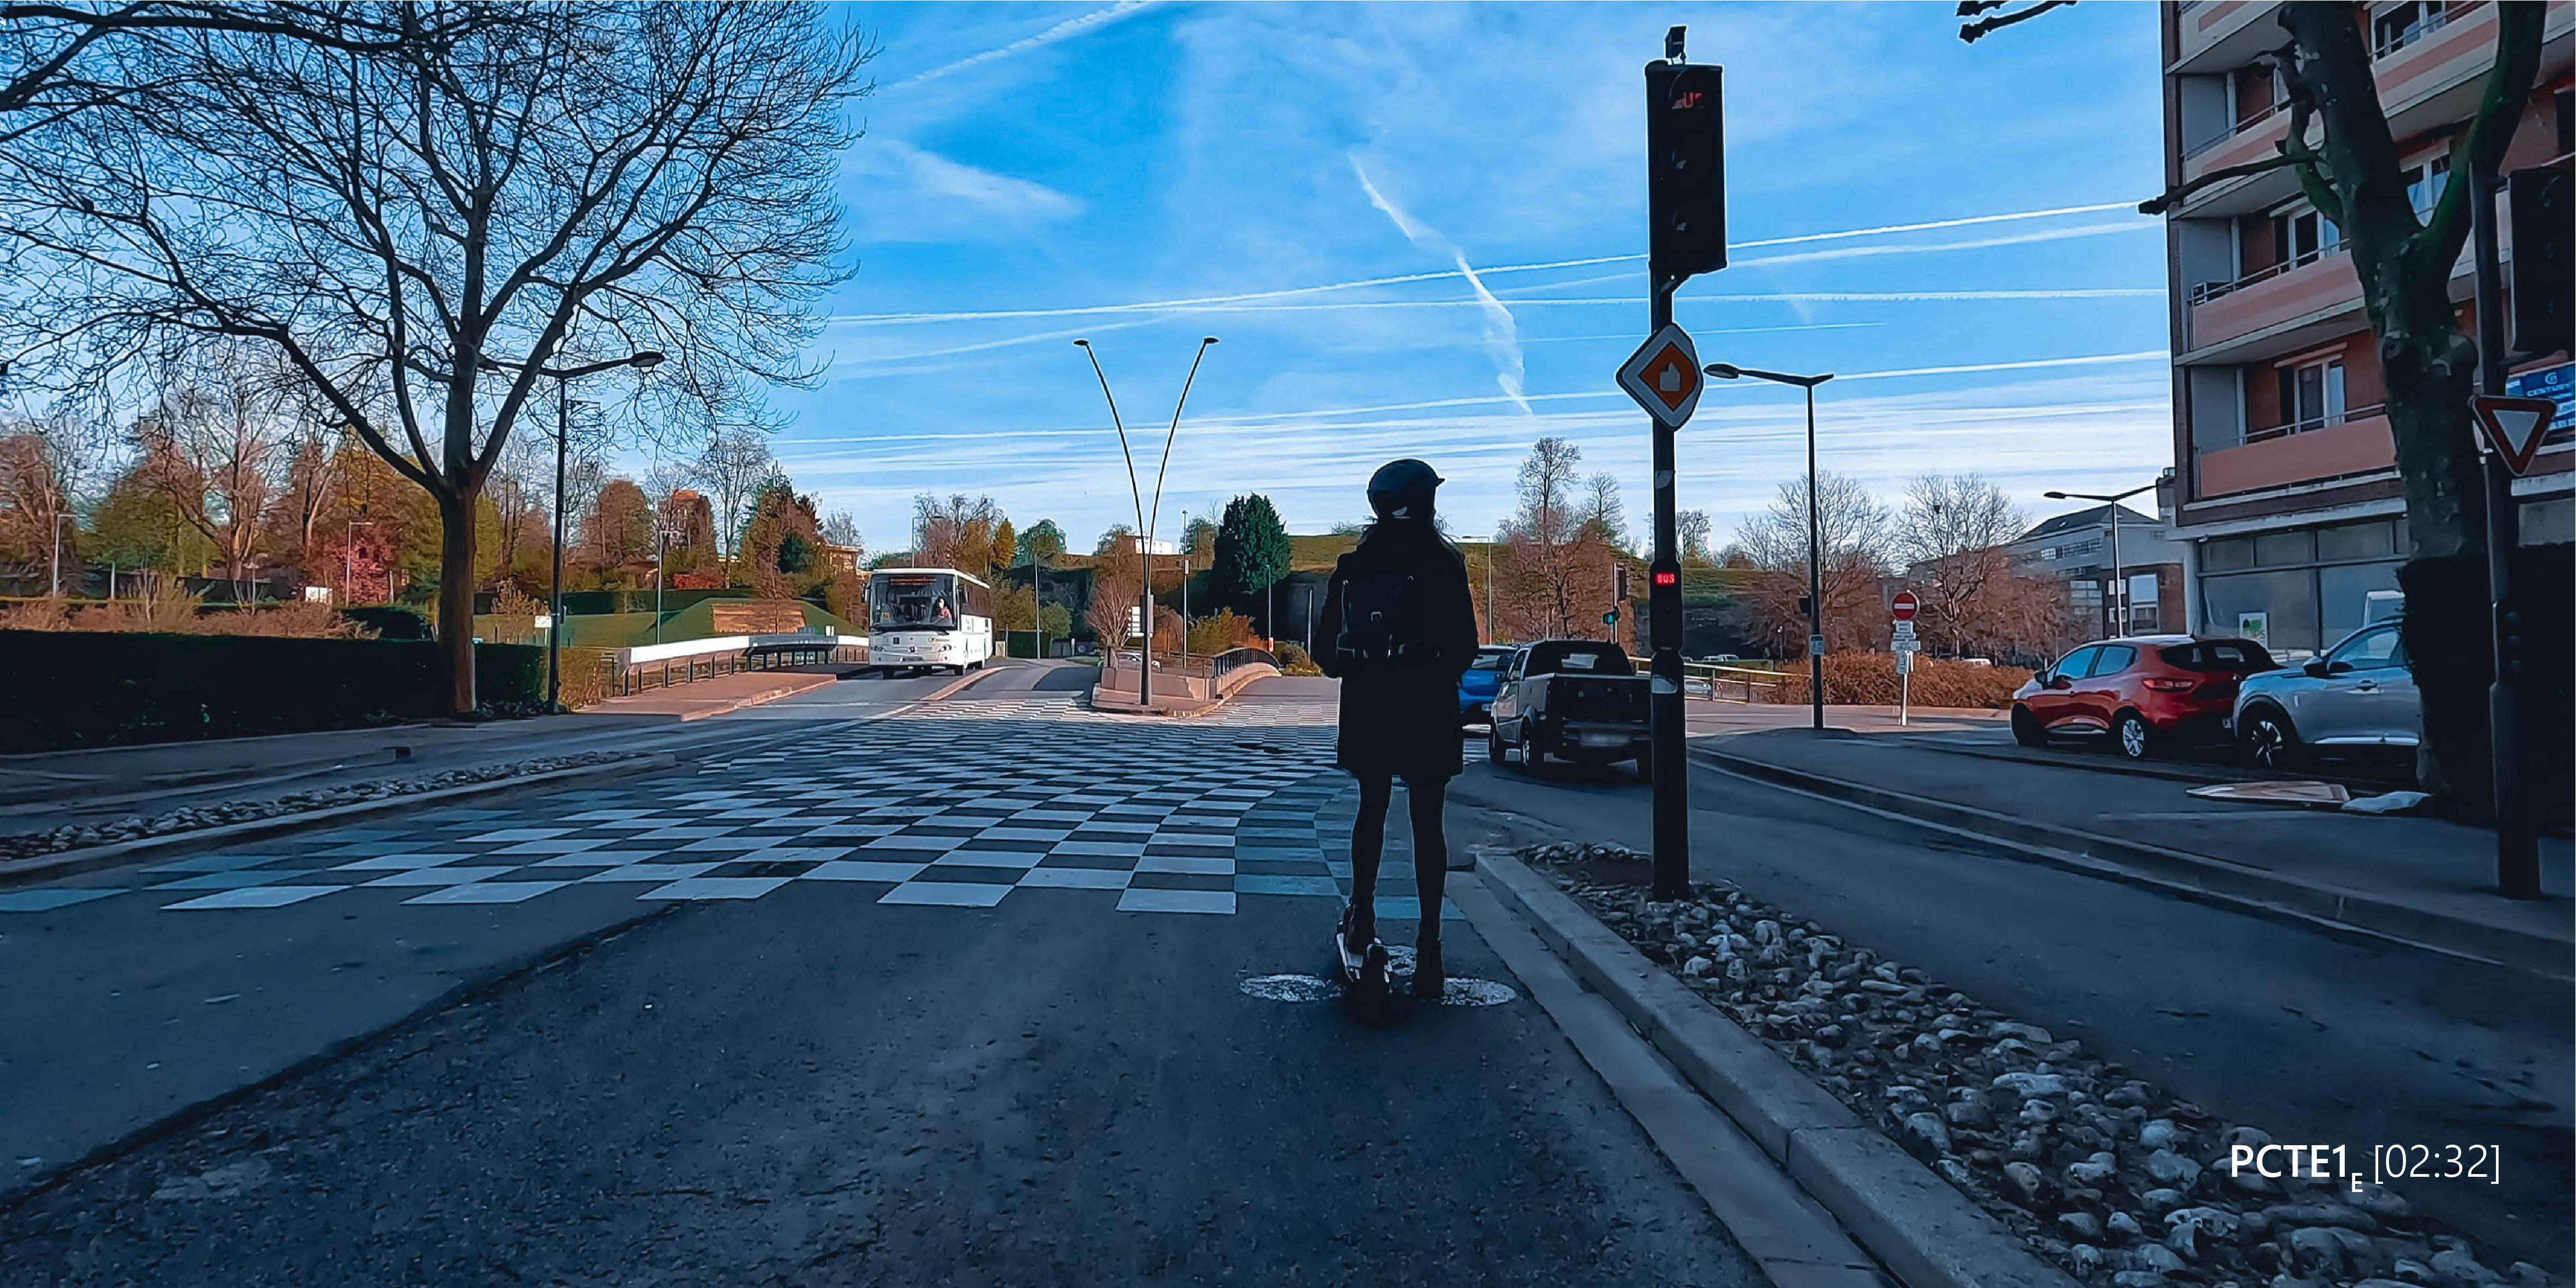
\includegraphics[width=0.75\columnwidth]{src/Figures/Annexes/Extrait_Video_PCTE1_Egress_5.jpg}}
        \vspace{5pt}
        \begin{flushright}\scriptsize{
        Auteur~: \textcolor{blue}{Dylan Moinse (2022)}
        }\end{flushright}
    \end{figure}

    % PCTE1 Photo Egress 6
    \begin{figure}[h!]\vspace*{4pt}
        \caption*{Extrait n°6 de la vidéo lors du trajet en diffusion (\(PCTE^{E}_{1}\))}
        \centerline{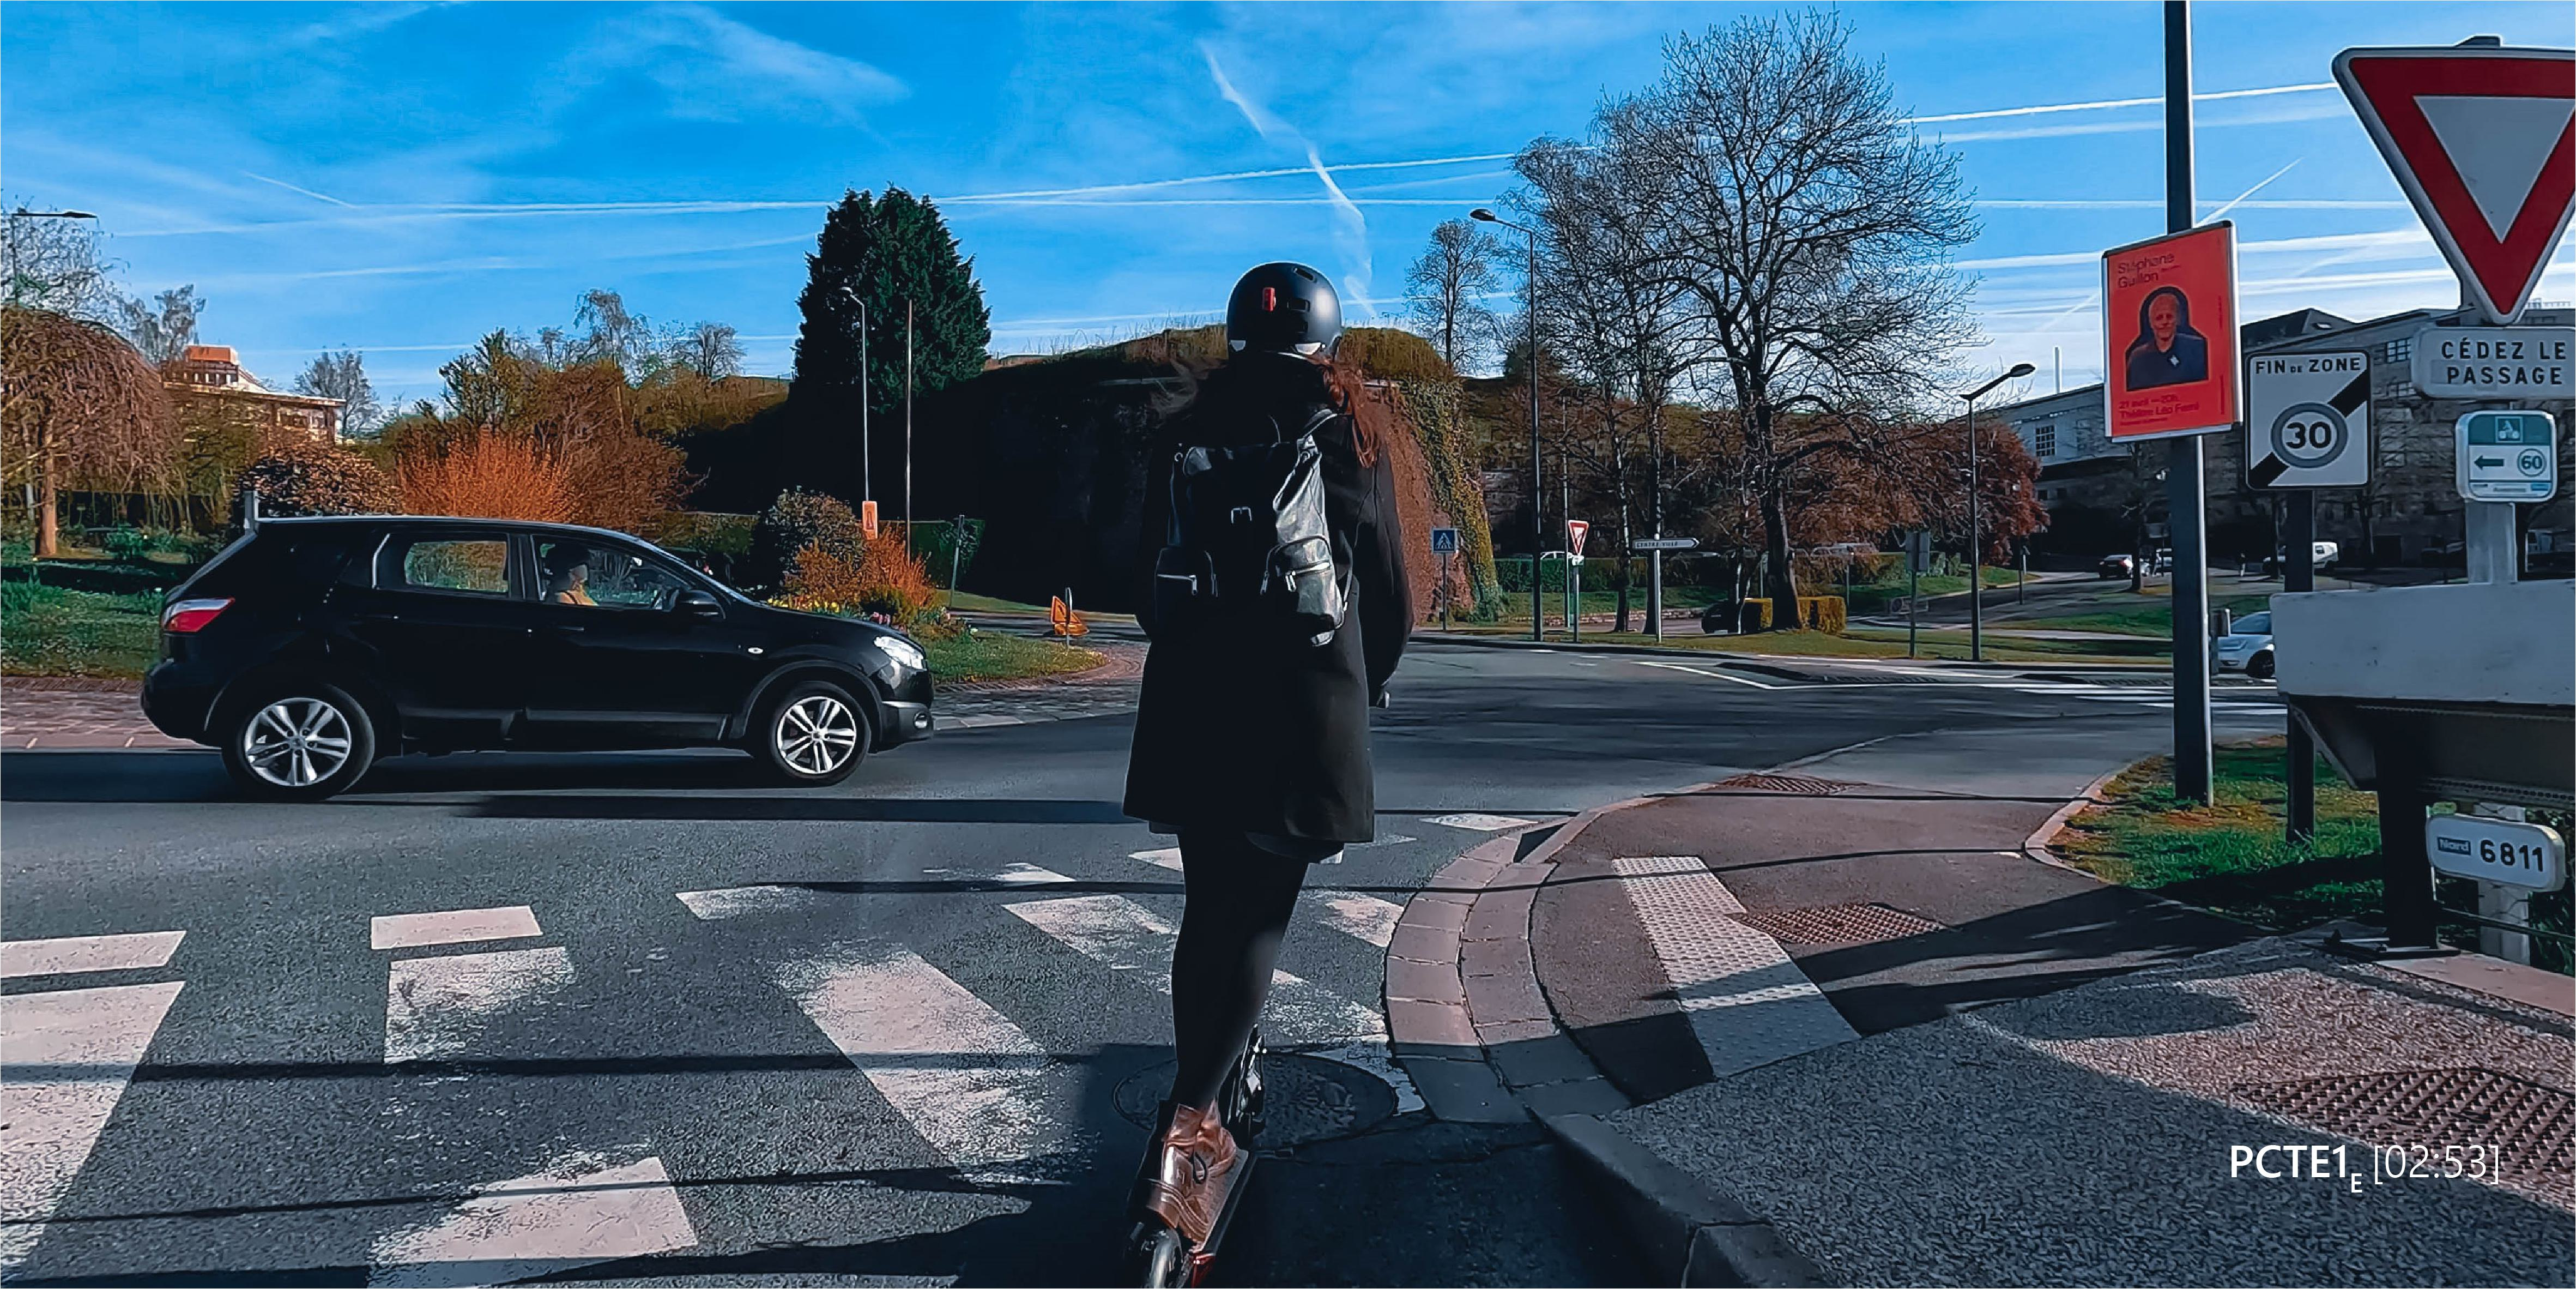
\includegraphics[width=0.75\columnwidth]{src/Figures/Annexes/Extrait_Video_PCTE1_Egress_6.jpg}}
        \vspace{5pt}
        \begin{flushright}\scriptsize{
        Auteur~: \textcolor{blue}{Dylan Moinse (2022)}
        }\end{flushright}
    \end{figure}

    % PCTE1 Photo Egress 7
    \begin{figure}[h!]\vspace*{4pt}
        \caption*{Extrait n°7 de la vidéo lors du trajet en diffusion (\(PCTE^{E}_{1}\))}
        \centerline{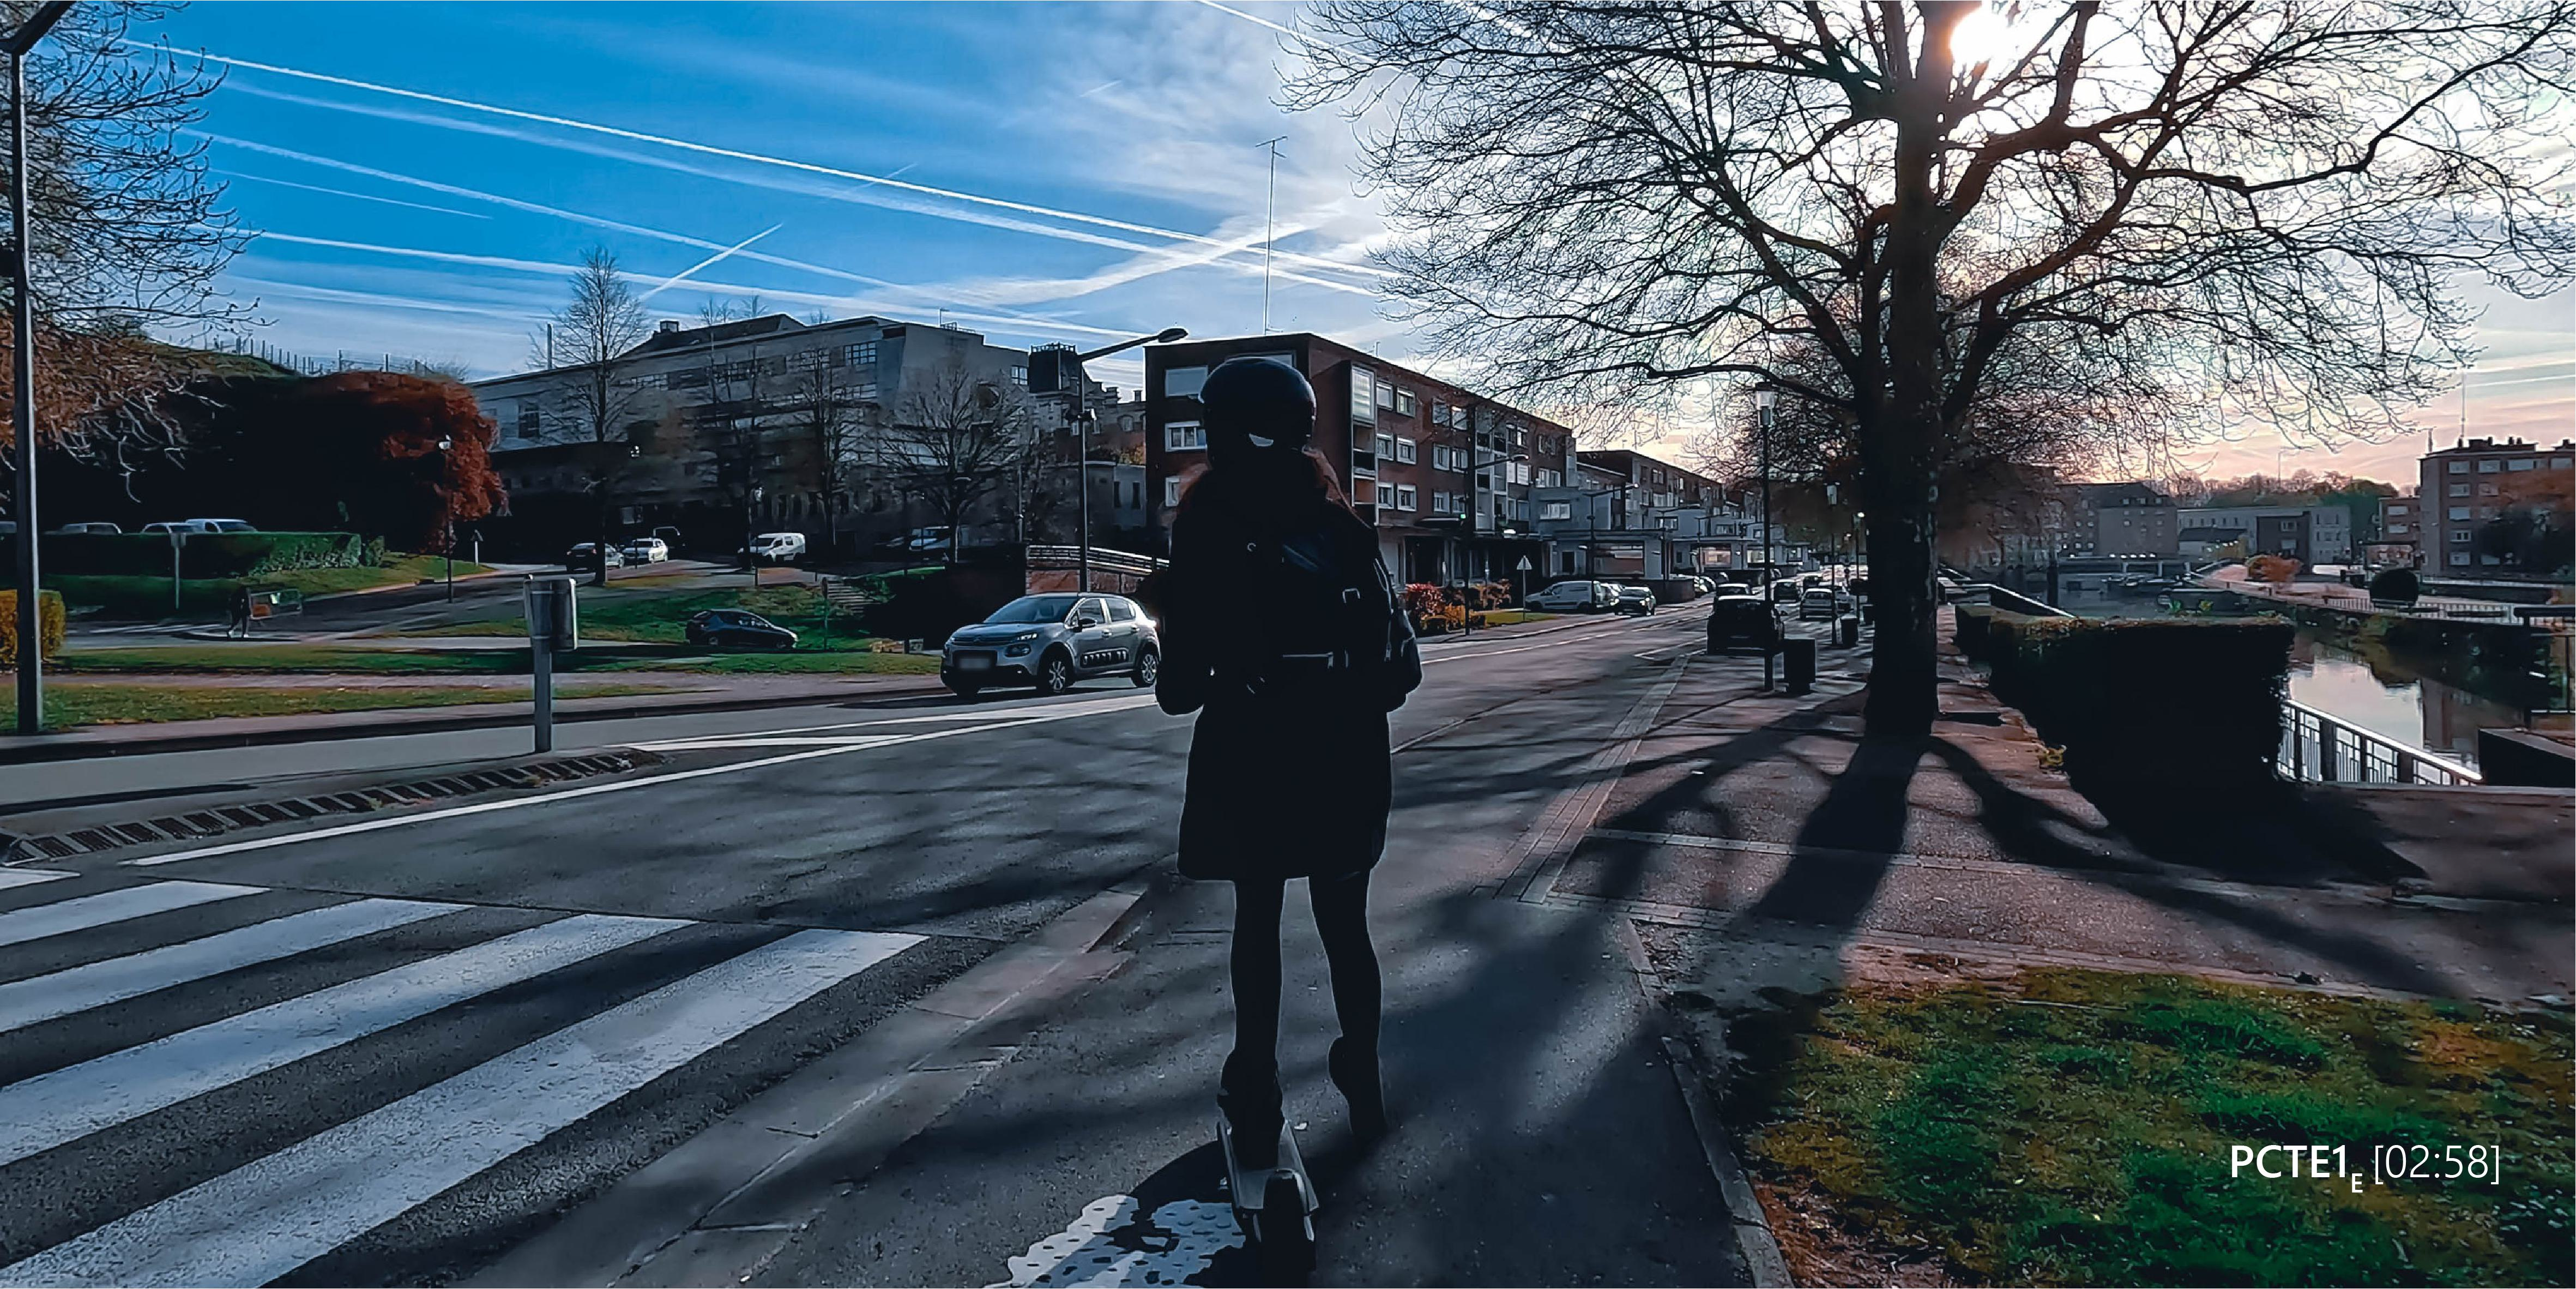
\includegraphics[width=0.75\columnwidth]{src/Figures/Annexes/Extrait_Video_PCTE1_Egress_7.jpg}}
        \vspace{5pt}
        \begin{flushright}\scriptsize{
        Auteur~: \textcolor{blue}{Dylan Moinse (2022)}
        }\end{flushright}
    \end{figure}

    % PCTE1 Photo Egress 8
    \begin{figure}[h!]\vspace*{4pt}
        \caption*{Extrait n°8 de la vidéo lors du trajet en diffusion (\(PCTE^{E}_{1}\))}
        \centerline{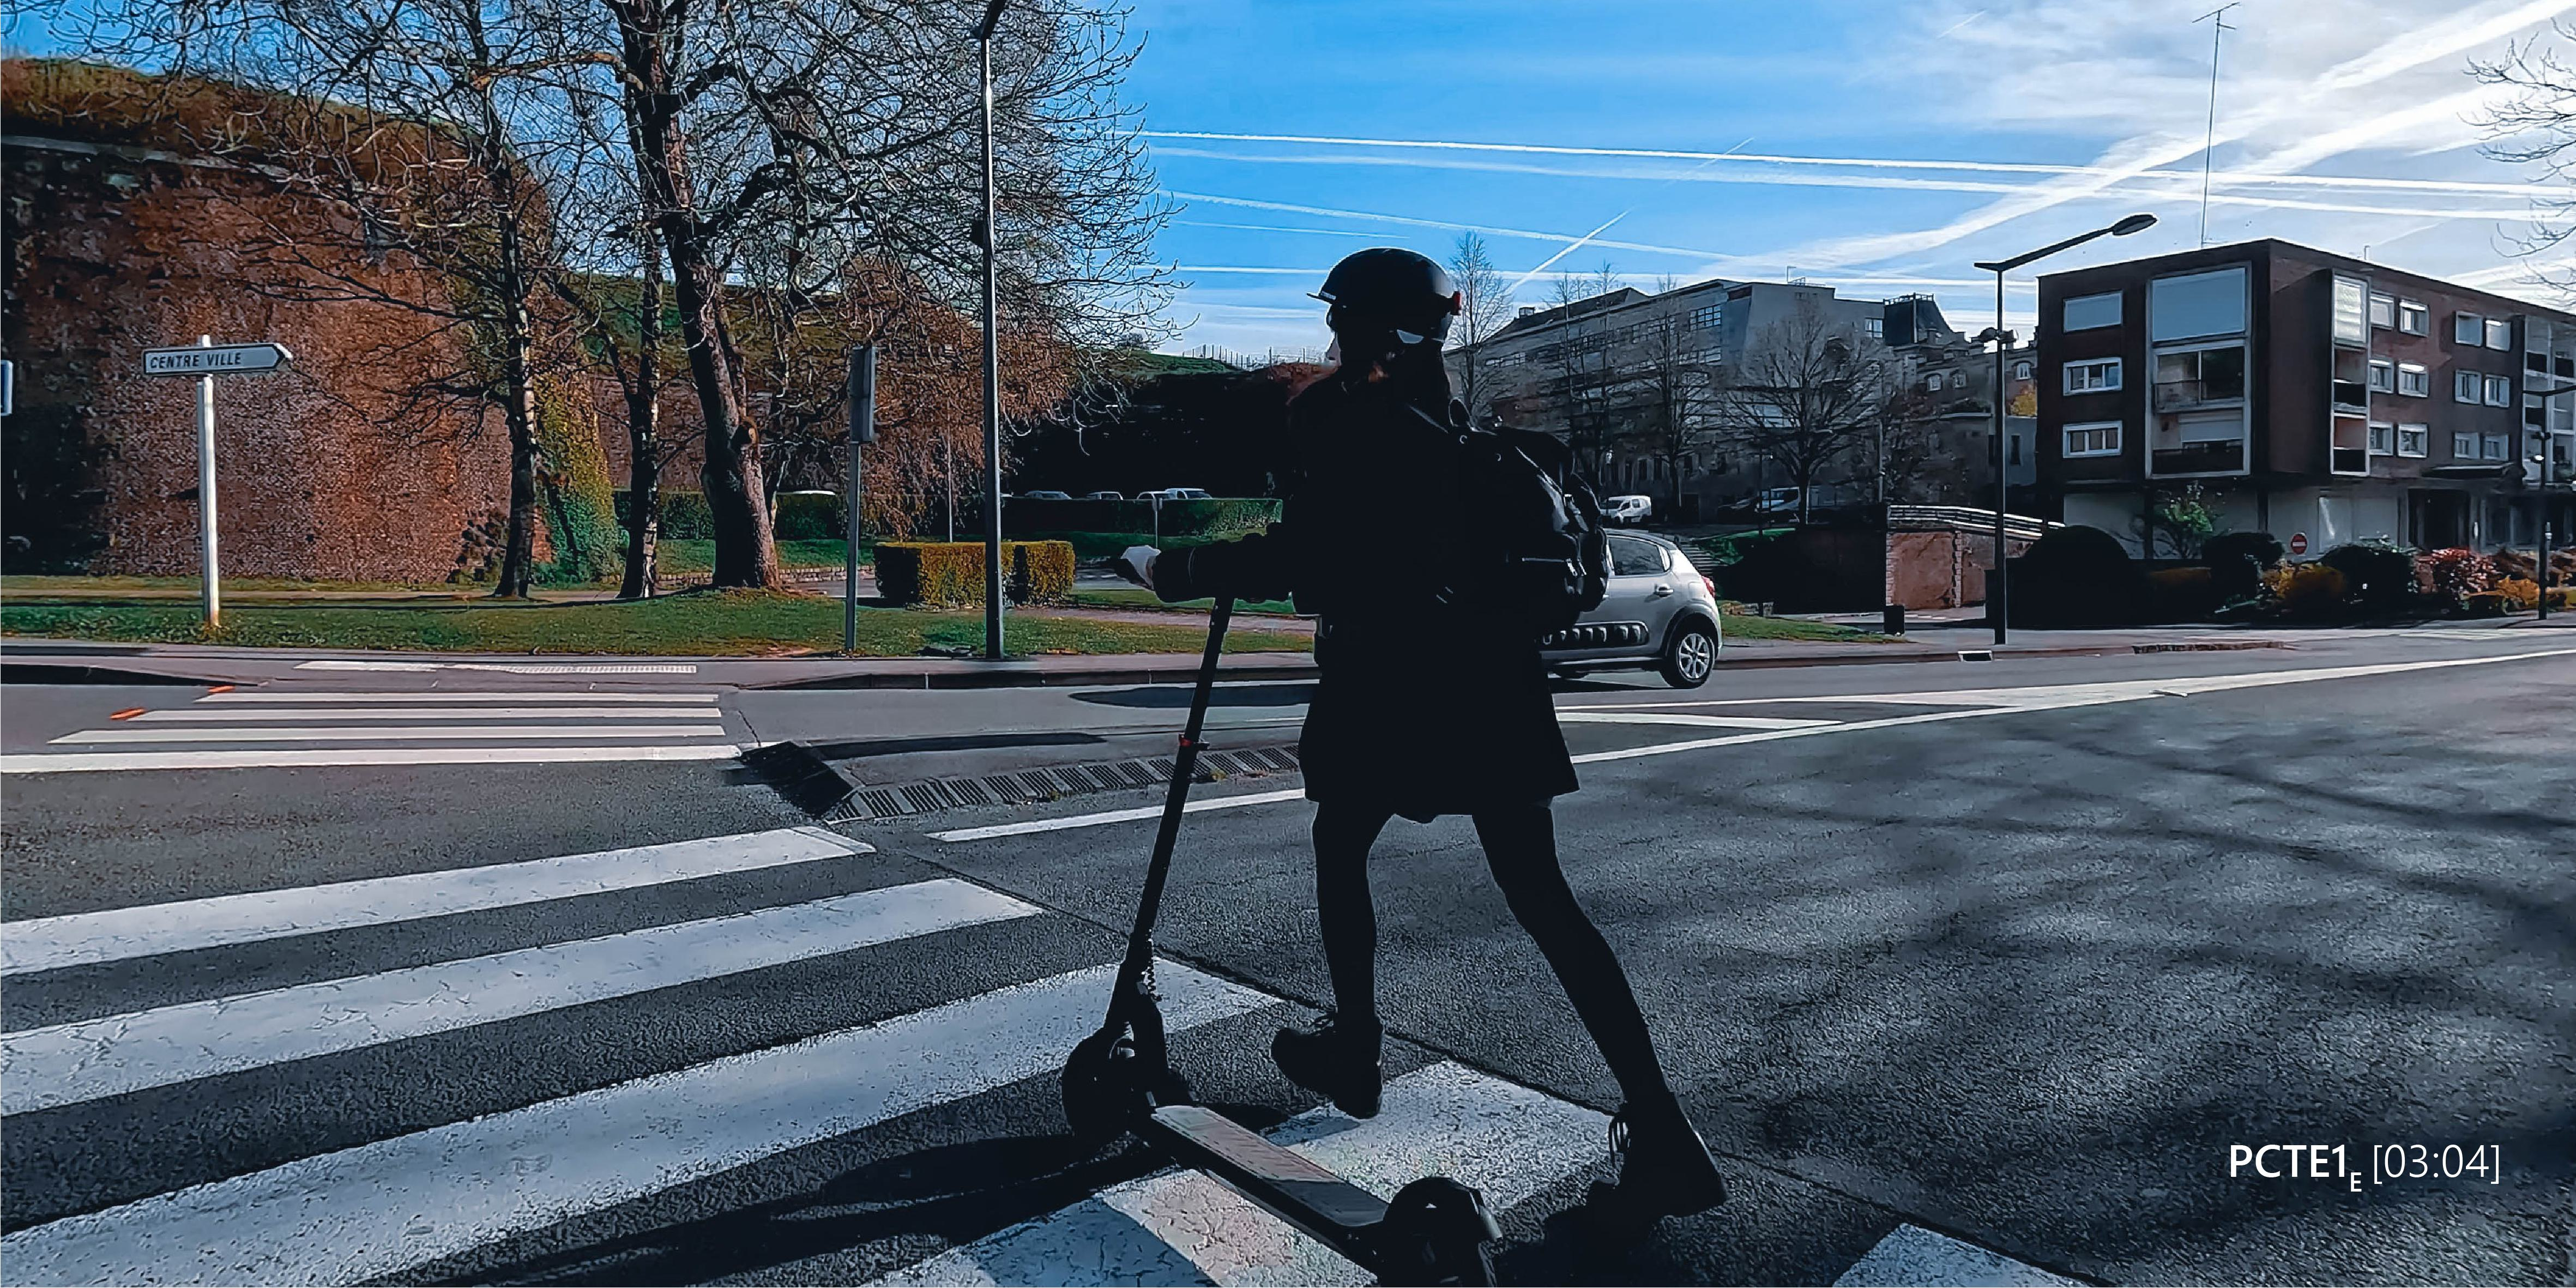
\includegraphics[width=0.75\columnwidth]{src/Figures/Annexes/Extrait_Video_PCTE1_Egress_8.jpg}}
        \vspace{5pt}
        \begin{flushright}\scriptsize{
        Auteur~: \textcolor{blue}{Dylan Moinse (2022)}
        }\end{flushright}
    \end{figure}

    % PCTE1 Photo Egress 9
    \begin{figure}[h!]\vspace*{4pt}
        \caption*{Extrait n°9 de la vidéo lors du trajet en diffusion (\(PCTE^{E}_{1}\))}
        \centerline{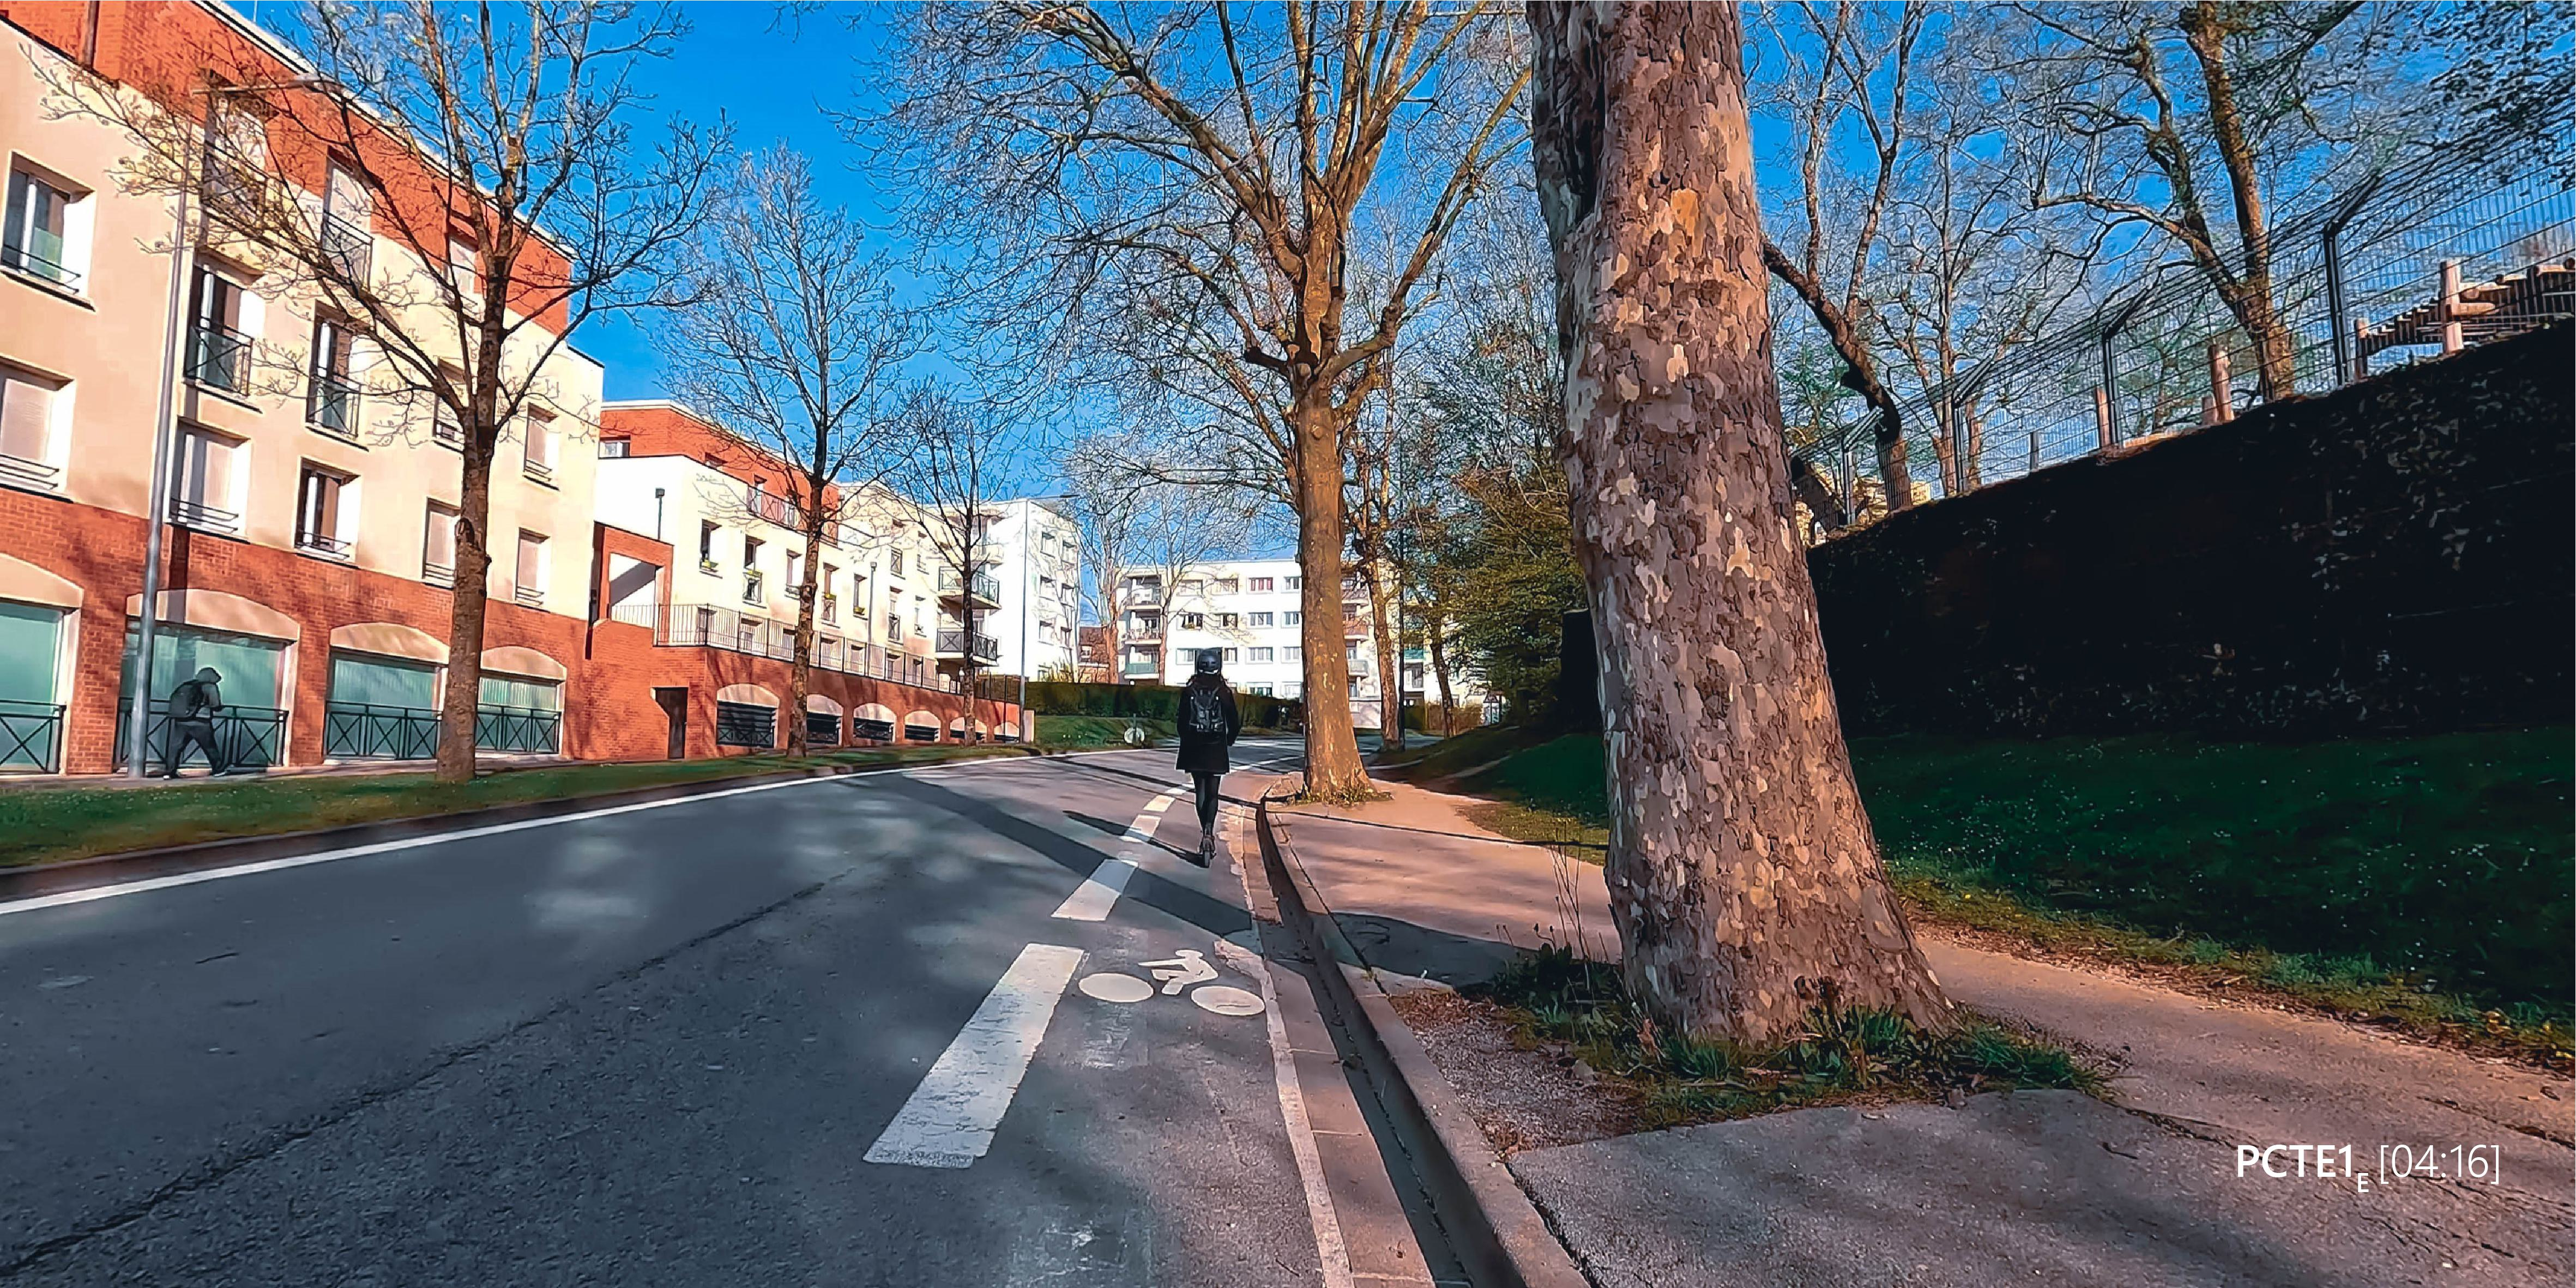
\includegraphics[width=0.75\columnwidth]{src/Figures/Annexes/Extrait_Video_PCTE1_Egress_9.jpg}}
        \vspace{5pt}
        \begin{flushright}\scriptsize{
        Auteur~: \textcolor{blue}{Dylan Moinse (2022)}
        }\end{flushright}
    \end{figure}

    % PCTE1 Photo Egress 10
    \begin{figure}[h!]\vspace*{4pt}
        \caption*{Extrait n°10 de la vidéo lors du trajet en diffusion (\(PCTE^{E}_{1}\))}
        \centerline{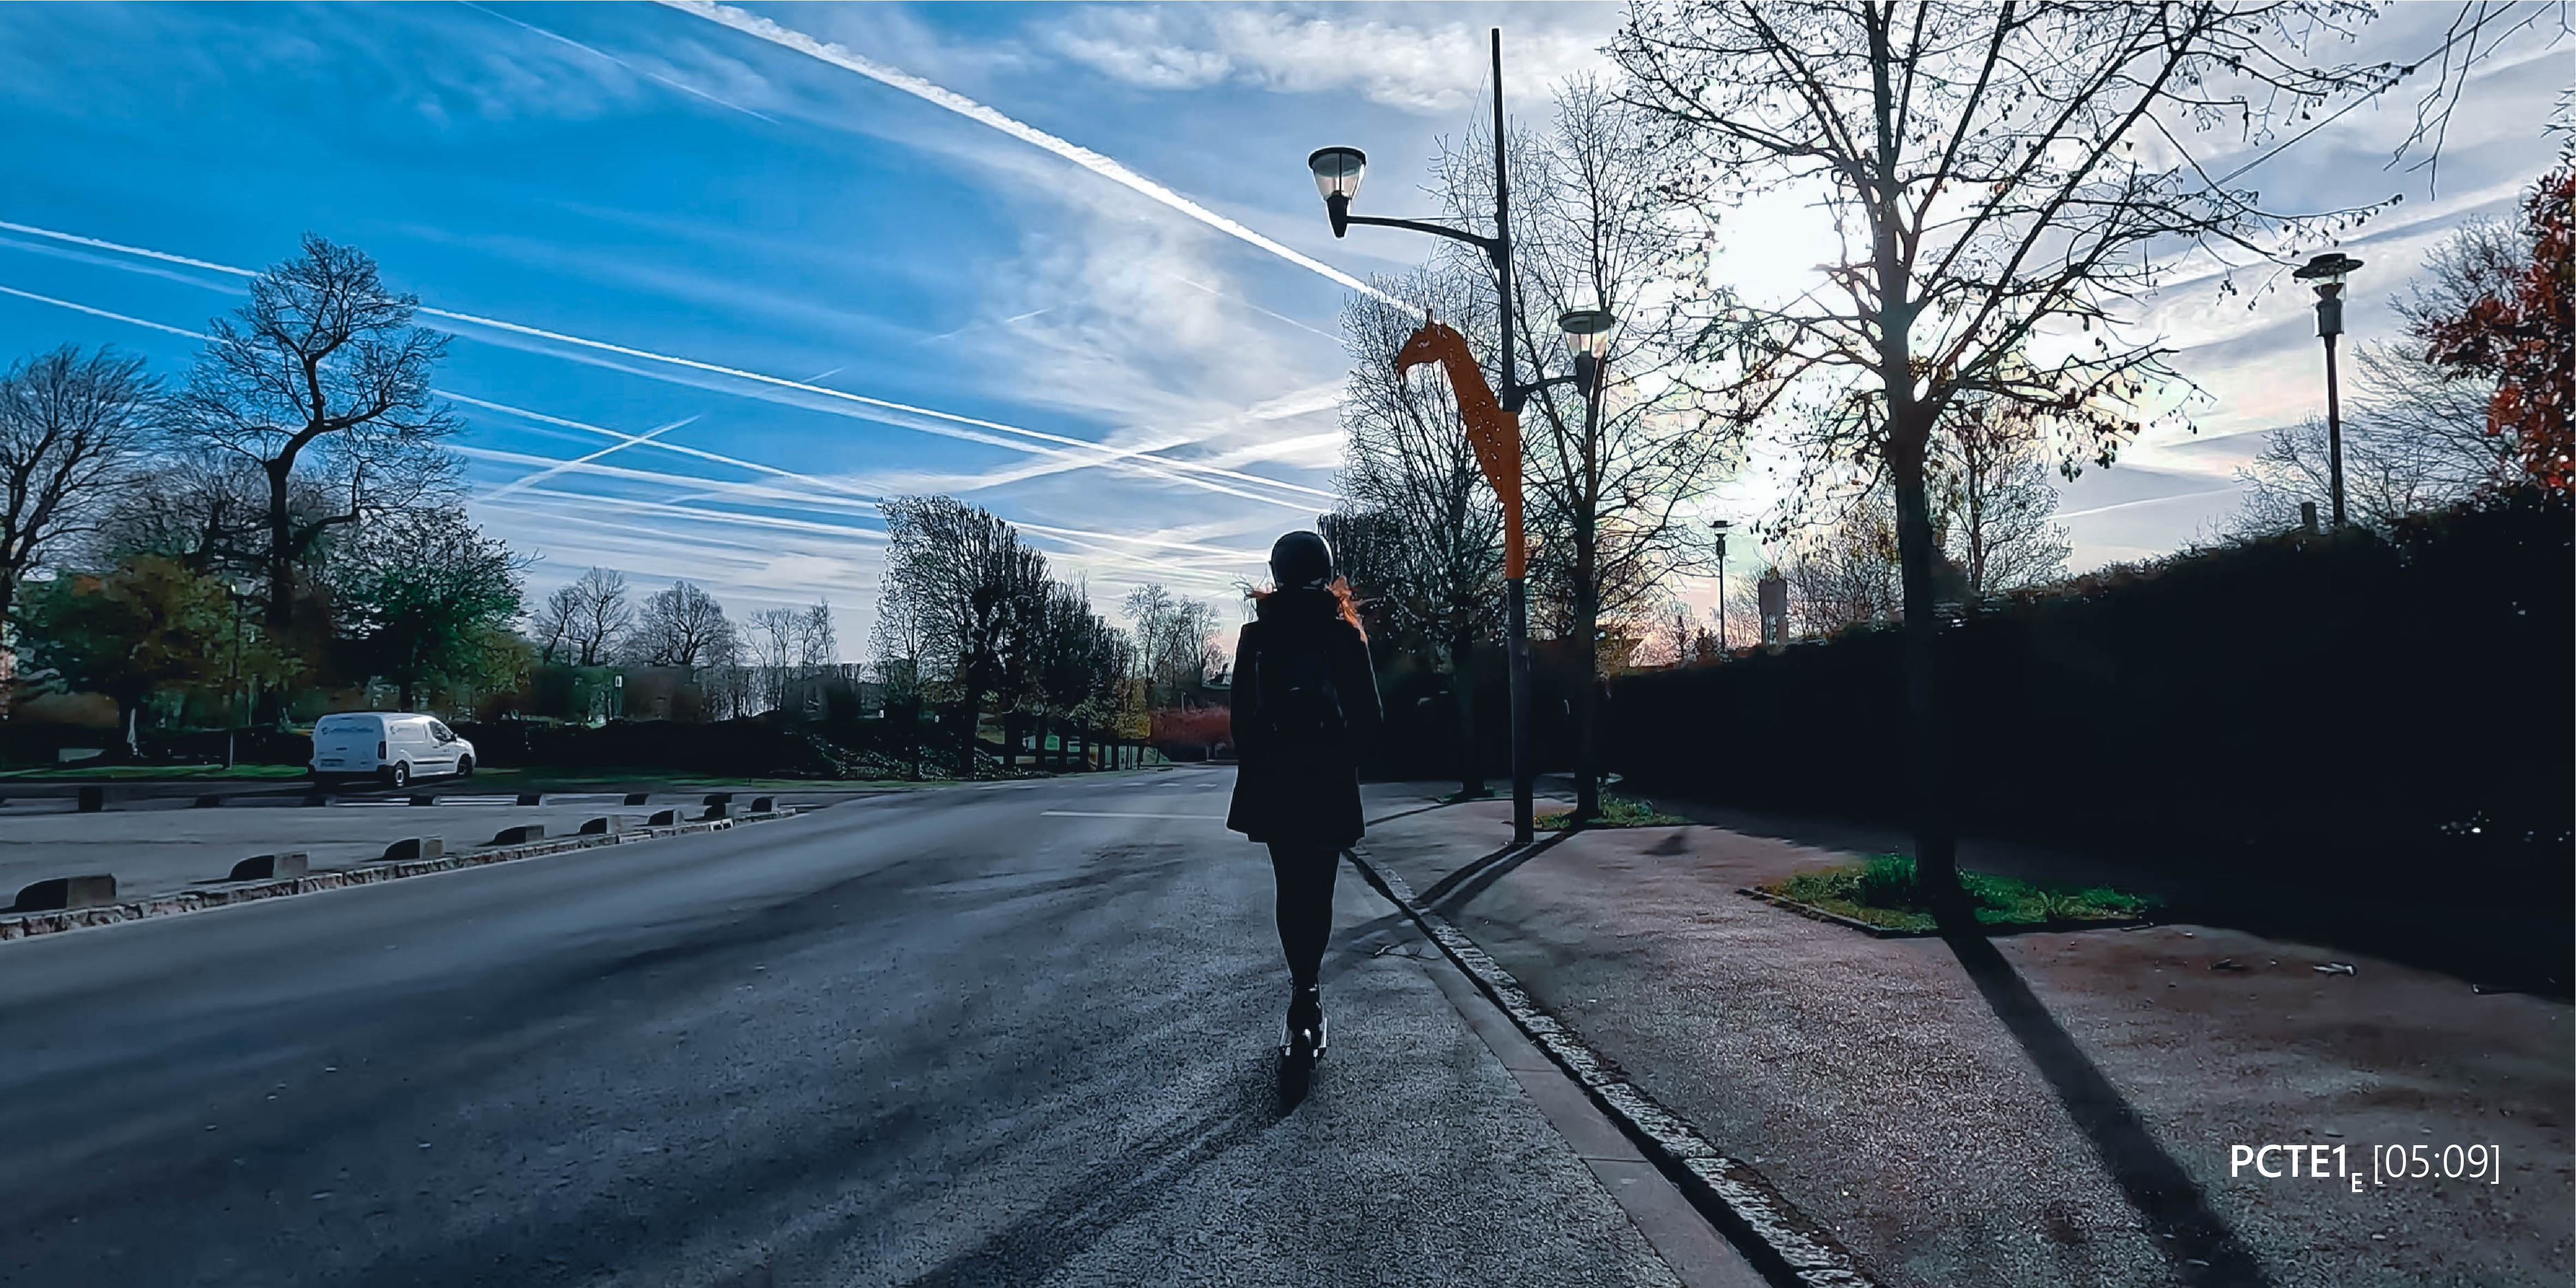
\includegraphics[width=0.75\columnwidth]{src/Figures/Annexes/Extrait_Video_PCTE1_Egress_10.jpg}}
        \vspace{5pt}
        \begin{flushright}\scriptsize{
        Auteur~: \textcolor{blue}{Dylan Moinse (2022)}
        }\end{flushright}
    \end{figure}

    % Retranscription PCTE2
    \newpage
    \needspace{1\baselineskip} % Réserve de l'espace
    \sectionheader{Retranscription du second parcours commenté}
\section{Retranscription du second parcours commenté}
    \label{annexes:retranscription-pcte2}

    % Retranscription PCTE2 rabattement
\subsection{Échanges retranscrits durant le trajet en rabattement en trottinette électrique}

\begin{description}
    \item[Participant \(PCTE^{A}_{2}\)] [00:27]~: Là, je vais continuer tout droit parce que si je tourne à droite, je \textsl{me tape} une rue avec des pavés. Une bande cyclable [à la place du stationnement automobile] suffirait dans cette rue, car elle est pas hyper passante.
    \item[Participant \(PCTE^{A}_{2}\)] [00:58]~: En \textsl{V'Lille}, ça me dérange moins les pavés, mais là\dots~\textsl{Nan}\dots~pas en trottinette.
    \item[Participant \(PCTE^{A}_{2}\)] [02:00]~: Ça ne me dérange pas tant que ça de rouler avec les voitures, tu vois. Par contre, je me retrouve collé aux voitures stationnées sur le côté de la route, et j'ai toujours peur de me prendre une portière ouverte.
    \item[Participant \(PCTE^{A}_{2}\)] [02:44]~: Lors du retour, je suis pas satisfait par les flèches cyclables à contre-sens [le double sens cyclable], car il y a toujours des voitures qui sont mal garées. C'est stressant quand on croise une voiture, car il faut avoir de la place pour circuler face à elle. Souvent, je m'arrête face à une voiture.
    \item[Participant \(PCTE^{A}_{2}\)] [03:15]~: Là, je vais sur le SAS vélo. C'est pratique pour tourner à gauche. On n'est pas entre les voitures.
    \item[Participant \(PCTE^{A}_{2}\)] [04:45]~: \textsl{Là}, il y a beaucoup de sorties de garages dans cette rue et les gens ne font pas très attention. J'aime pas les bandes cyclables à côté de voitures garées à cause des portières. Et sur le bout de la rue, on sait pas quoi faire. Moi qui arrive au métro, je dois continuer tout droit sur le passage piéton et sur le trottoir.%%Rédigé%%
\end{description}

    % Retranscription PCTE2 TC
\subsection{Échanges retranscrits durant le trajet en métro}

\begin{description}
    \item[Participant \(PCTE^{TC}_{2}\)] [00:03]~: \textsl{Hop~!} Les escalateurs, c'est bien, car ça m'évite de porter le poids de la trottinette dans les escaliers. Mais ce n'est pas non plus optimal, car je dois trouver la bonne prise de la trottinette. Je prends pas l'ascenseur du métro, car c'est pour les PMR [Personnes à Mobilité Réduite] en général et, car c'est \textsl{malfamé}.
    \item[Participant \(PCTE^{TC}_{2}\)] [03:29]~: Je suis obligé de rester dans le carré central du métro parce qu'il n'y a pas de place ailleurs. Si je reste assis, il y a pas de place pour mettre ma trottinette. Donc, je reste debout avec ma trottinette. Je préfère être aussi dans cette place centrale, car si j'étais contre une porte, je devrais bouger dès qu'elle s'ouvre.%%Rédigé%%
    
    Idéalement, je coince ma route contre la barre du métro et je me tiens à l'aide du guidon pour tenir dans le métro. C'est la meilleure technique que j'ai, car on peut pas vraiment la poser sans qu'elle tombe et dérange tout le monde. Au moins, je gêne moins comme ça, je trouve.%%Rédigé%%

    \item[Participant \(PCTE^{TC}_{2}\)] [04:20]~: J'ai choisi une trottinette justement qui ne pèse pas très lourd, pour pouvoir la porter facilement dans les endroits où je peux pas rouler, comme dans les escaliers ou dans le métro.
    \item[Participant \(PCTE^{TC}_{2}\)] [04:39]~: Comme j'ai des horaires flexibles, je vais étudier plus tôt pour éviter les heures de pointe, car sinon il y a pas de place pour aller en trottinette.
    \item[Participant \(PCTE^{TC}_{2}\)] [05:02]~: Quand on arrive à mon bâtiment principal qui est mon bureau, le bâtiment \textsl{X} et l'autre \textsl{Y} où je travaille et où j'ai cours souvent.
    \item[Enquêteur] [05:20]~: Donc, occasionnellement, tu te rends dans un autre bâtiment du campus grâce à ta trottinette électrique~?
    \item[Participant \(PCTE^{TC}_{2}\)] [05:25]~: C'est ça. Au moins une fois par semaine, souvent deux fois.
    \item[Enquêteur] [05:32]~: Tu peux m'expliquer plus en détails le déplacement qu'on fait en trottinette et en métro~?
    \item[Participant \(PCTE^{TC}_{2}\)] [05:35]~: \textsl{En gros}, je passe toujours à \textsl{X} récupérer mes affaires, comme la blouse, mon ordinateur, \textsl{et tout}. Et ensuite, je repars jusqu'à \textsl{Y}. C'est agréable de circuler en \textsl{trotti.} sur le campus.
    \item[Enquêteur] [06:02]~: Tu peux me décrire ce que tu entends par \textsl{agréable}~?
    \item[Participant \(PCTE^{TC}_{2}\)] [06:09]~: C'est tranquille en général. \textsl{Mais en même temps\dots~Non.} Il n’y a aucune place donnée aux vélos et aux trottinettes sur le campus. Mais, c’est vrai qu’on est vite limité parce qu’on ne sait jamais par où passer. Dès qu’on passe par la route, entre les voitures garées sur le côté et les rues qui sont étroites, on se sent vite oppressé par les voitures derrière nous. C’est vrai qu’on doit aussi jongler entre les piétons.
    \item[Enquêteur] [07:26]~: Et pourquoi pas reprendre le métro pour aller de \textsl{X} à \textsl{Y}~?
    \item[Participant \(PCTE^{TC}_{2}\)] [07:38]~: Pour le coup, ce serait plus rapide que j’y aille à pied. Pour aller au métro, il faudrait que je retourne à \textsl{Cité Scientifique} [la station d'arrivée], que j’attende le métro et que j’aille à \textsl{4 Cantons} [le terminus de la Ligne 1] pour marcher ensuite. Alors que là, je traverse rapidement le campus. En trottinette, je mets moins de cinq minutes alors qu’à pied, c’est au moins vingt minutes. Surtout qu'après, je dois faire le retour, donc fois deux.
    \item[Enquêteur] [08:05]~: Donc, pour toi, le métro est efficace pour de longues distances, comme le déplacement que l'on réalise entre \textsl{République - Beaux-Arts} et \textsl{Cité Scientifique}. Mais, il est moins intéressant lorsque tu fais face à des courtes distances, mais pas suffisamment pour les réaliser à pied, et que tu préfères faire en trottinette~?
    \item[Participant \(PCTE^{TC}_{2}\)] [08:20]~: Des courtes distances, avec des bâtiments qui sont pas à côté du métro. Si mes deux bâtiments étaient à côté des deux arrêts de métro, j'aurais pris le métro. Là, c'est pendant mon travail, je peux pas me permettre de perdre quarante minutes de marche. En trottinette, sur un aller-retour, je gagne plus de trente minutes. Franchement, j'irais en voiture si je devais marcher autant, ce serait plus simple. Et encore, je fais facilement plusieurs allers-retours [entre \textsl{X} et \textsl{Y}] dans une journée\dots~[Nous arrivons à destination, à l'arrêt \textsl{Cité Scientifique Pr. Gabillard}]%%Rédigé%%

    Après, la trottinette est pas très pratique. À cause des grillages, je roule sur les trottoirs car on a pas accès aux routes du campus.
    \item[Enquêteur] [08:38]~: On peut poursuivre la discussion en trottinette, mais avant, je dois mettre fin à cet entretien audio. Est-ce que tu as des commentaires ou des questions~?
    \item[Participant \(PCTE^{TC}_{2}\)] [08:44]~: Tout est bon pour moi.%%Rédigé%%
\end{description}

    % Entretien en Egress
\subsection{Échanges retranscrits durant le trajet en diffusion en trottinette électrique}

\begin{description}
    \item[Participant \(PCTE^{E}_{2}\)] [00:47]~: Je suis obligé de garder ma trottinette pliée en sortant du métro pour passer le portique. Je suis obligé de m'avancer \textsl{à fond} contre la porte, car elle détecte pas la présence de ma trottinette. Du coup, elle s'ouvre pas.%%Rédigé%%

    Les portiques sont pas assez larges pour que je marche à côté de ma trottinette. Et je sais pas comment fonctionne le portique pour les PMR.%%Rédigé%%

    C'était mieux avant, quand il y avait pas de portique. C'était plus fluide. Et pour les raisons évoquées. Il y a deux portiques de sortie pour une station de métro très fréquentée.
    \item[Participant \(PCTE^{E}_{2}\)] [02:03]~: Maintenant qu’on est arrivé à \textsl{Cité Scientifique} [la station d'arrivée], j’ai deux possibilités qui s’offrent à moi en termes de chemin. Soit passer par la route, soit passer par l’intérieur des bâtiments [les cheminements piétons au sein du campus]. Moi, je privilégie l’intérieur des bâtiments, car la route est plus agréable. La route sur le campus est pas adaptée pour les cyclistes et les \textsl{trottinettistes} [pointe du doigt l'Avenue Paul Langevin qui encercle le campus].
    \item[Participant \(PCTE^{E}_{2}\)] [03:13]~: Là, ce sont des nouveaux chemins qui viennent d’être faits et ils sont agréables. Ils ont été faits depuis cinq ou six mois, je dirais.
    \item[Participant \(PCTE^{E}_{2}\)] [03:19]~: Je dois contourner les piétons par contre, \textsl{c'est chiant.}
    \item[Participant \(PCTE^{E}_{2}\)] [03:29]~: \textsl{Là}, on va sur un sens interdit\dots~\textsl{On fait ce qu'on peut, hein.} C'est rare de voir des sens interdits, même pour les vélos. Il y a plein de place sur le campus. Si tu peux montrer \textsl{là-bas}, avec la caméra, le sens interdit. On voit qu'il y a de la place pour les voitures et de la place pour\dots~\textsl{on ne sait quoi.}%%Rédigé%%

    Ça pourrait être \textsl{clairement} un sens cyclable. Après, j’évite de passer par cette route [à sens unique] pour me rendre au bâtiment \textsl{Y} parce qu’il y a des dos d’âne vraiment pas agréables pour les \textsl{trottinettistes}. Je préfère passer par là [un cheminement parallèle] même si je dois descendre de la trottinette à un moment. Ça reste plus agréable.
    \item[Participant \(PCTE^{E}_{2}\)] [06:47]~: Cette route est \textsl{nulle.} On ne sait pas \textsl{où} est le trottoir et \textsl{où} est la route. À cause des zigzags, je me mets souvent sur le trottoir. Sinon, je dois attendre que la voiture en face passe. Comme le trottoir est large, je sais pas si c'est partagé [entre les piéton·ne·s et les cyclistes].%%Rédigé%%
\end{description}

    % Photos PCTE2
    \newpage
\subsection{Sélection d'images extraites du second parcours commenté}
    \label{annexes:photos-pcte2}

    % Photos PCTE2 rabattement
\subsubsection{Sélection d'images extraites lors du trajet en rabattement}

    % PCTE2 Photo Access 1
    \begin{figure}[h!]\vspace*{4pt}
        \caption*{Extrait n°1 de la vidéo lors du trajet en rabattement (\(PCTE^{A}_{2}\))}
        \centerline{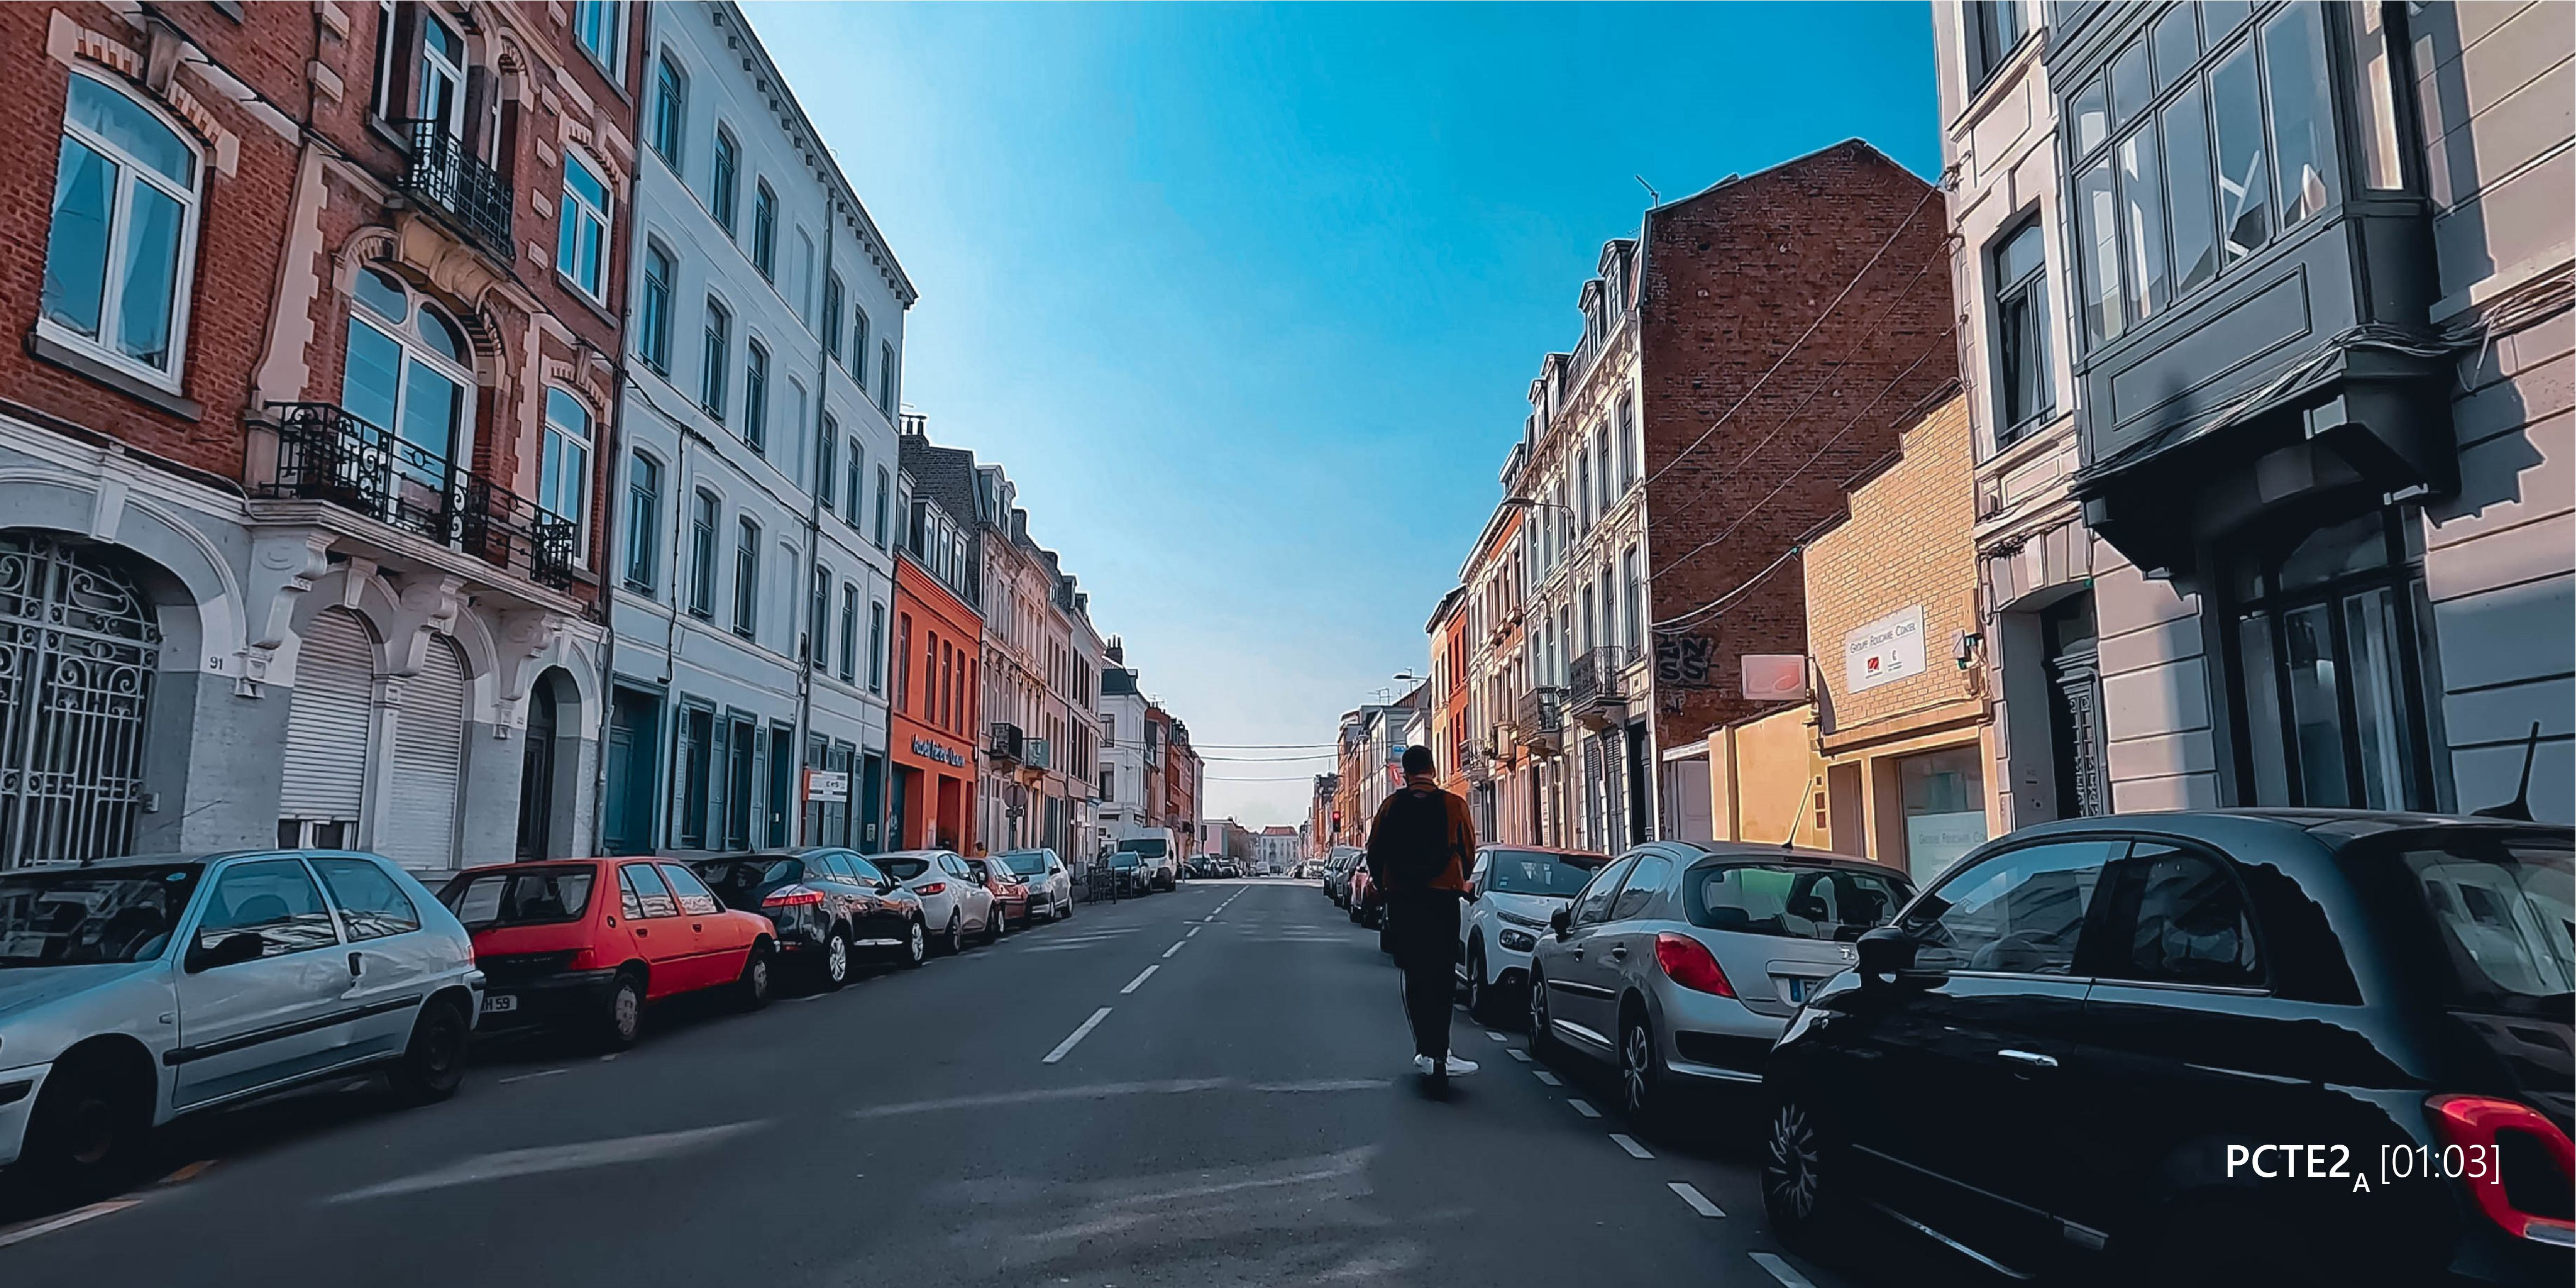
\includegraphics[width=0.75\columnwidth]{src/Figures/Annexes/Extrait_Video_PCTE2_Access_1.jpg}}
        \vspace{5pt}
        \begin{flushright}\scriptsize{
        Auteur~: \textcolor{blue}{Dylan Moinse (2022)}
        }\end{flushright}
    \end{figure}

    % PCTE2 Photo Access 2
    \begin{figure}[h!]\vspace*{4pt}
        \caption*{Extrait n°2 de la vidéo lors du trajet en rabattement (\(PCTE^{A}_{2}\))}
        \centerline{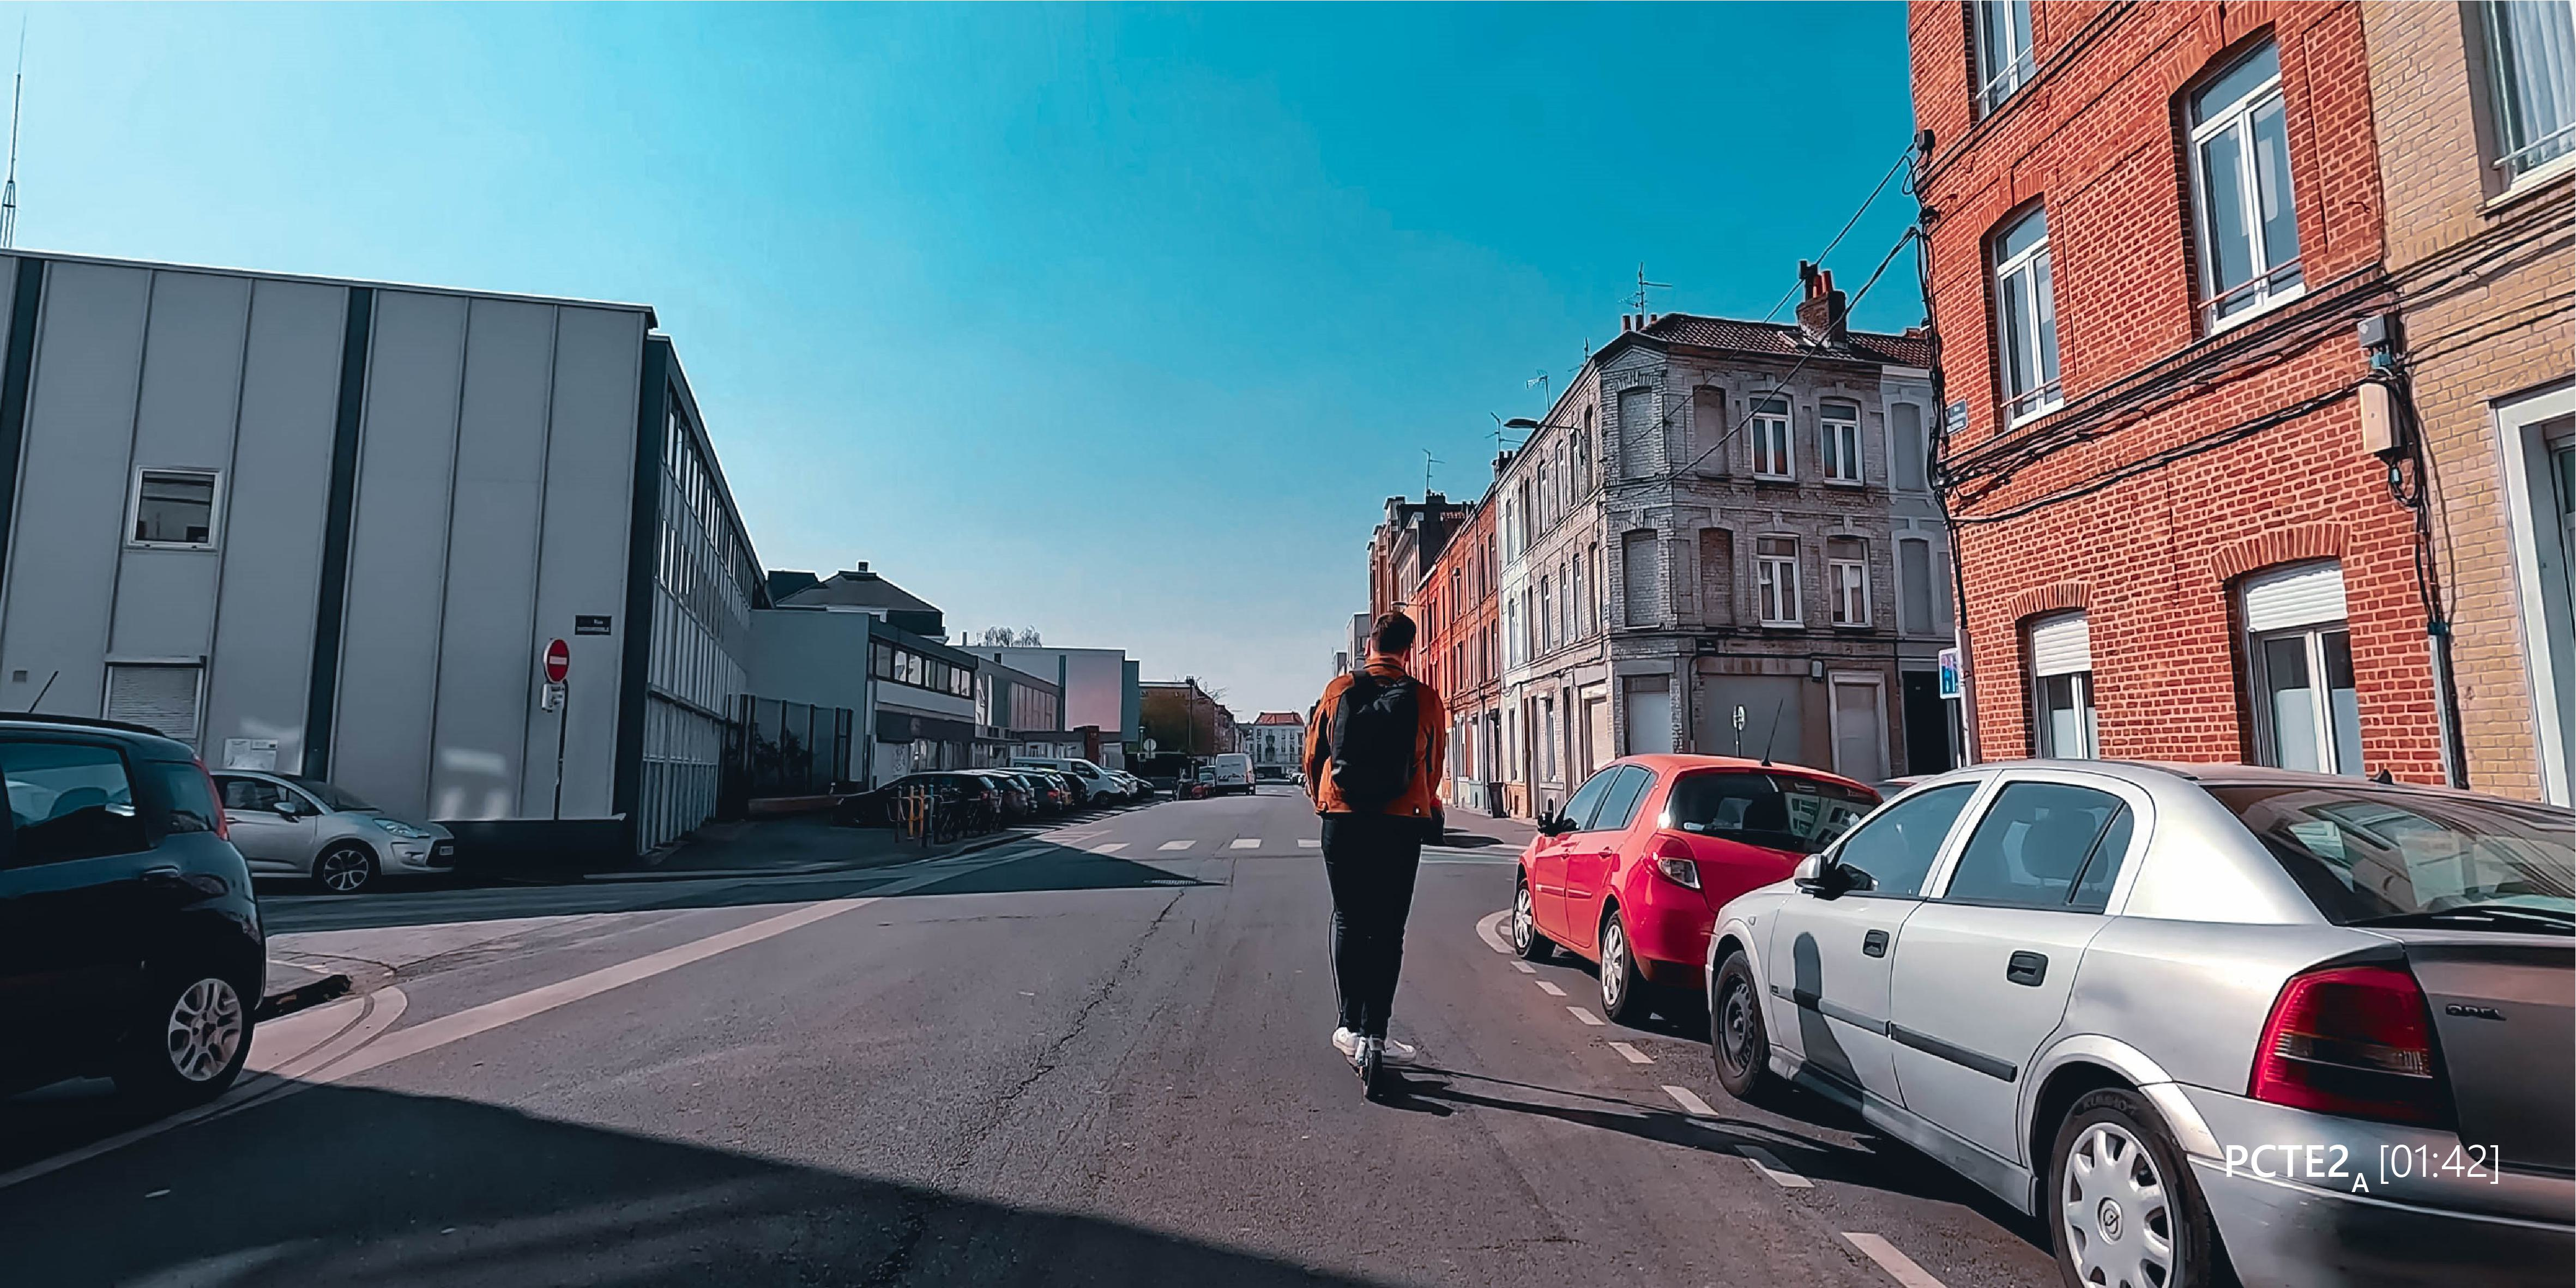
\includegraphics[width=0.75\columnwidth]{src/Figures/Annexes/Extrait_Video_PCTE2_Access_2.jpg}}
        \vspace{5pt}
        \begin{flushright}\scriptsize{
        Auteur~: \textcolor{blue}{Dylan Moinse (2022)}
        }\end{flushright}
    \end{figure}
    
    % PCTE2 Photo Access 3
    \begin{figure}[h!]\vspace*{4pt}
        \caption*{Extrait n°3 de la vidéo lors du trajet en rabattement (\(PCTE^{A}_{2}\))}
        \centerline{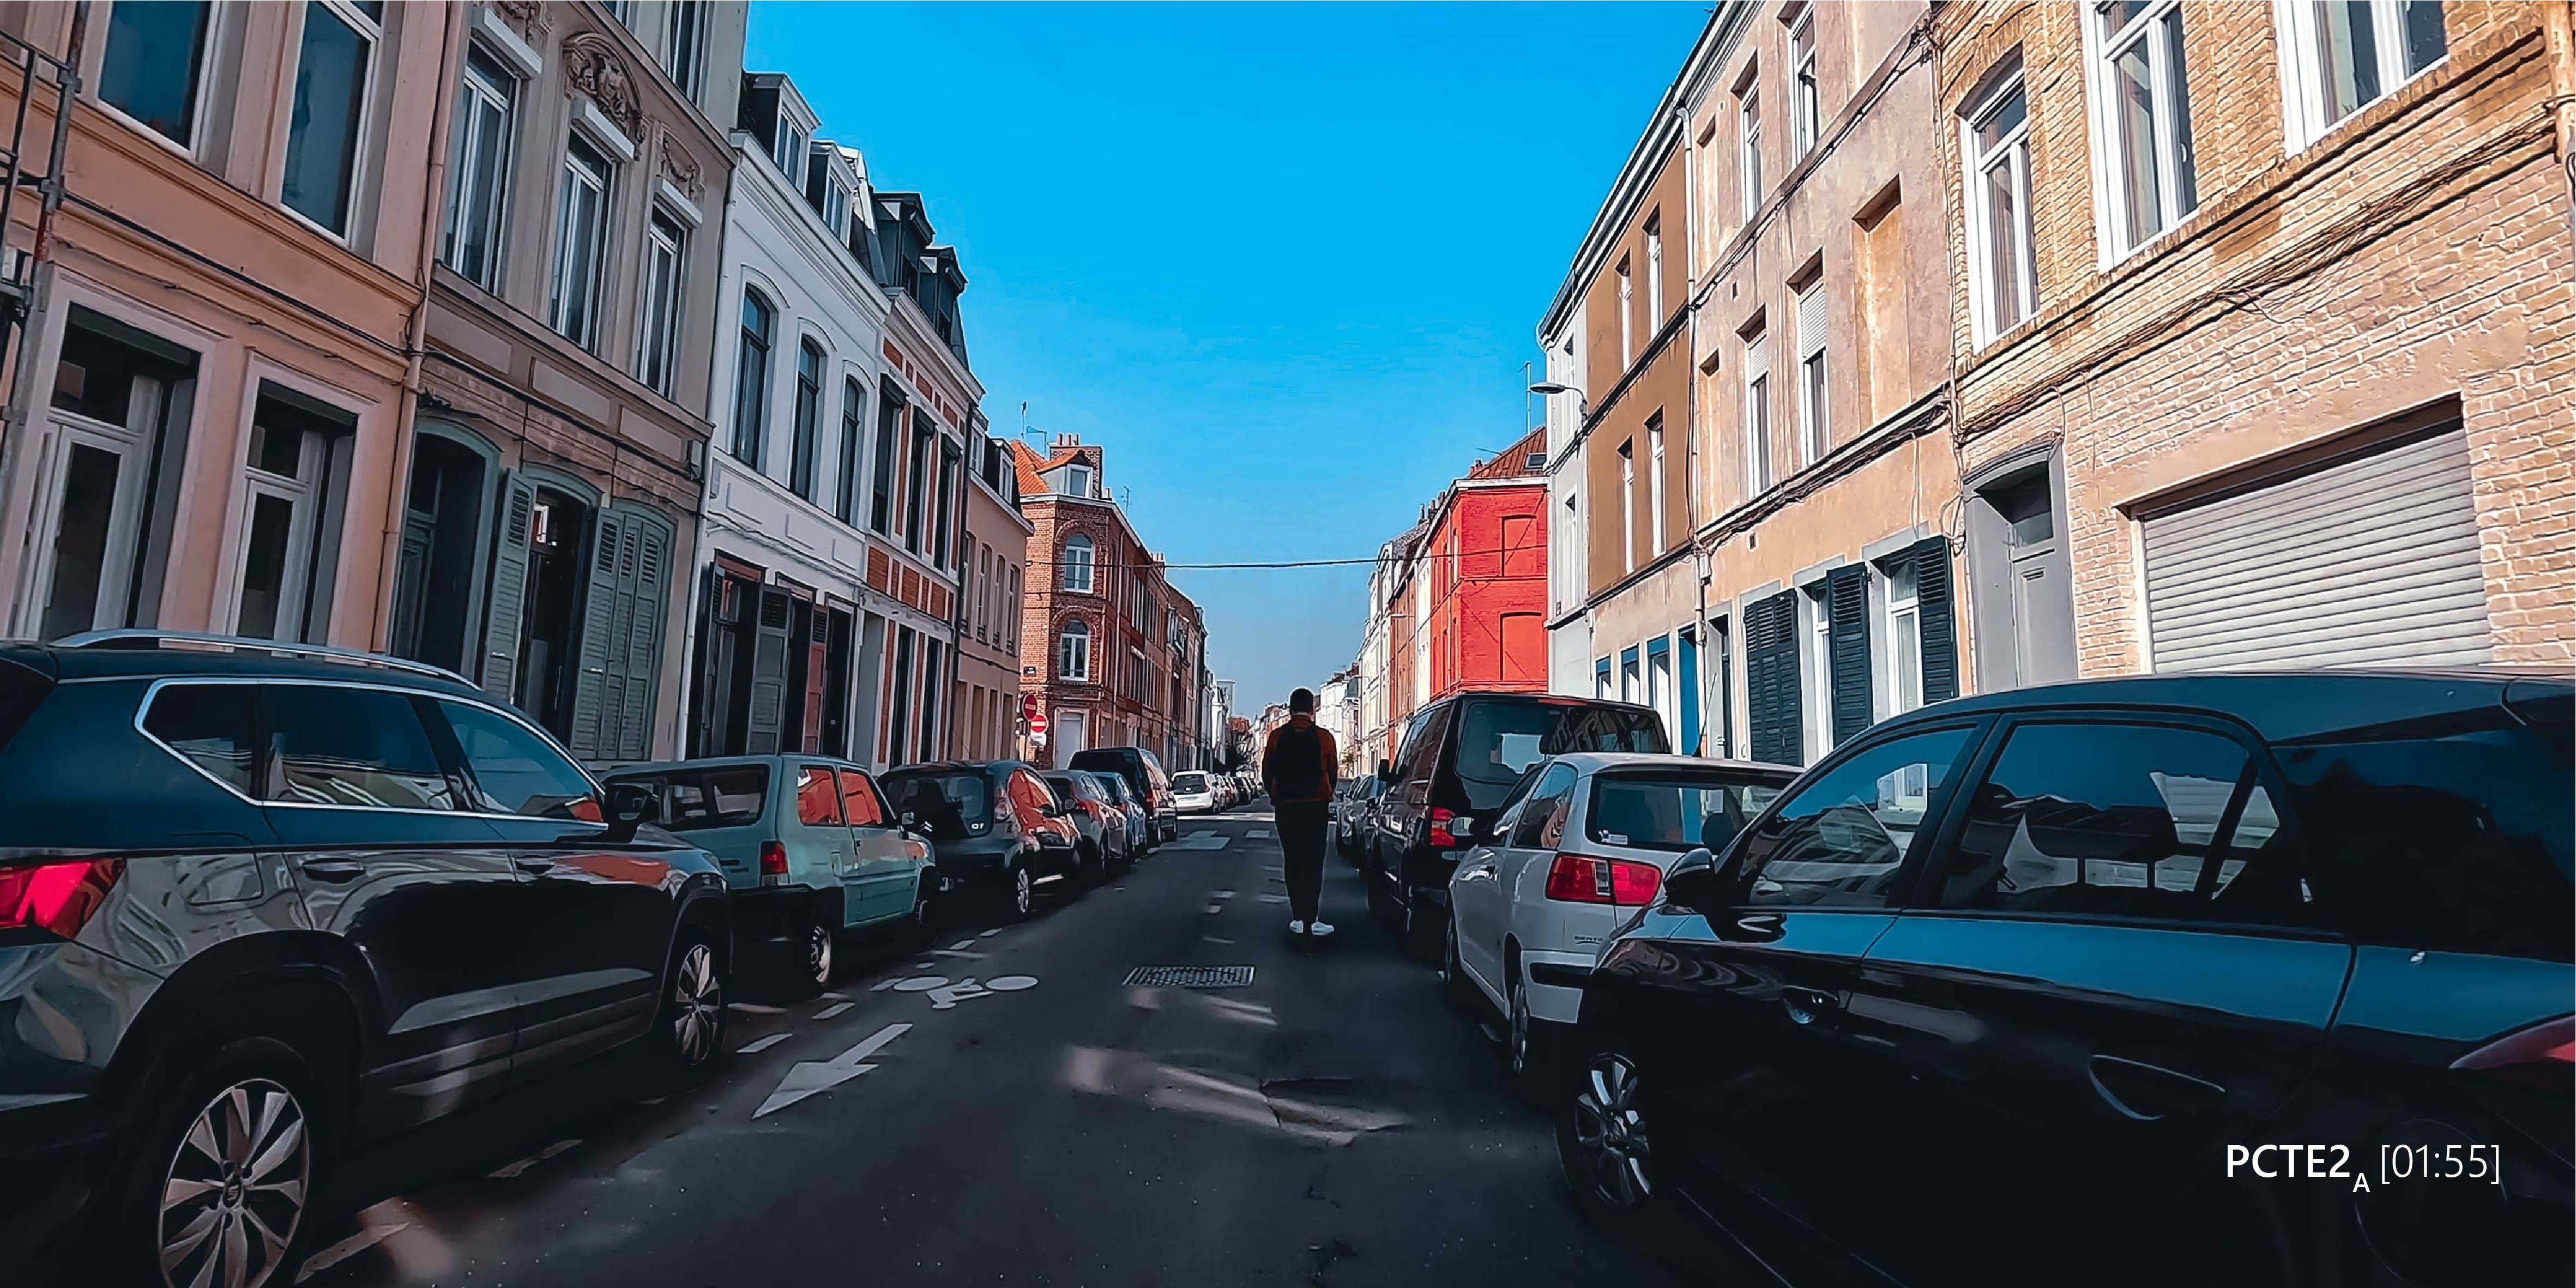
\includegraphics[width=0.75\columnwidth]{src/Figures/Annexes/Extrait_Video_PCTE2_Access_3.jpg}}
        \vspace{5pt}
        \begin{flushright}\scriptsize{
        Auteur~: \textcolor{blue}{Dylan Moinse (2022)}
        }\end{flushright}
    \end{figure}

    % PCTE2 Photo Access 4
    \begin{figure}[h!]\vspace*{4pt}
        \caption*{Extrait n°4 de la vidéo lors du trajet en rabattement (\(PCTE^{A}_{2}\))}
        \centerline{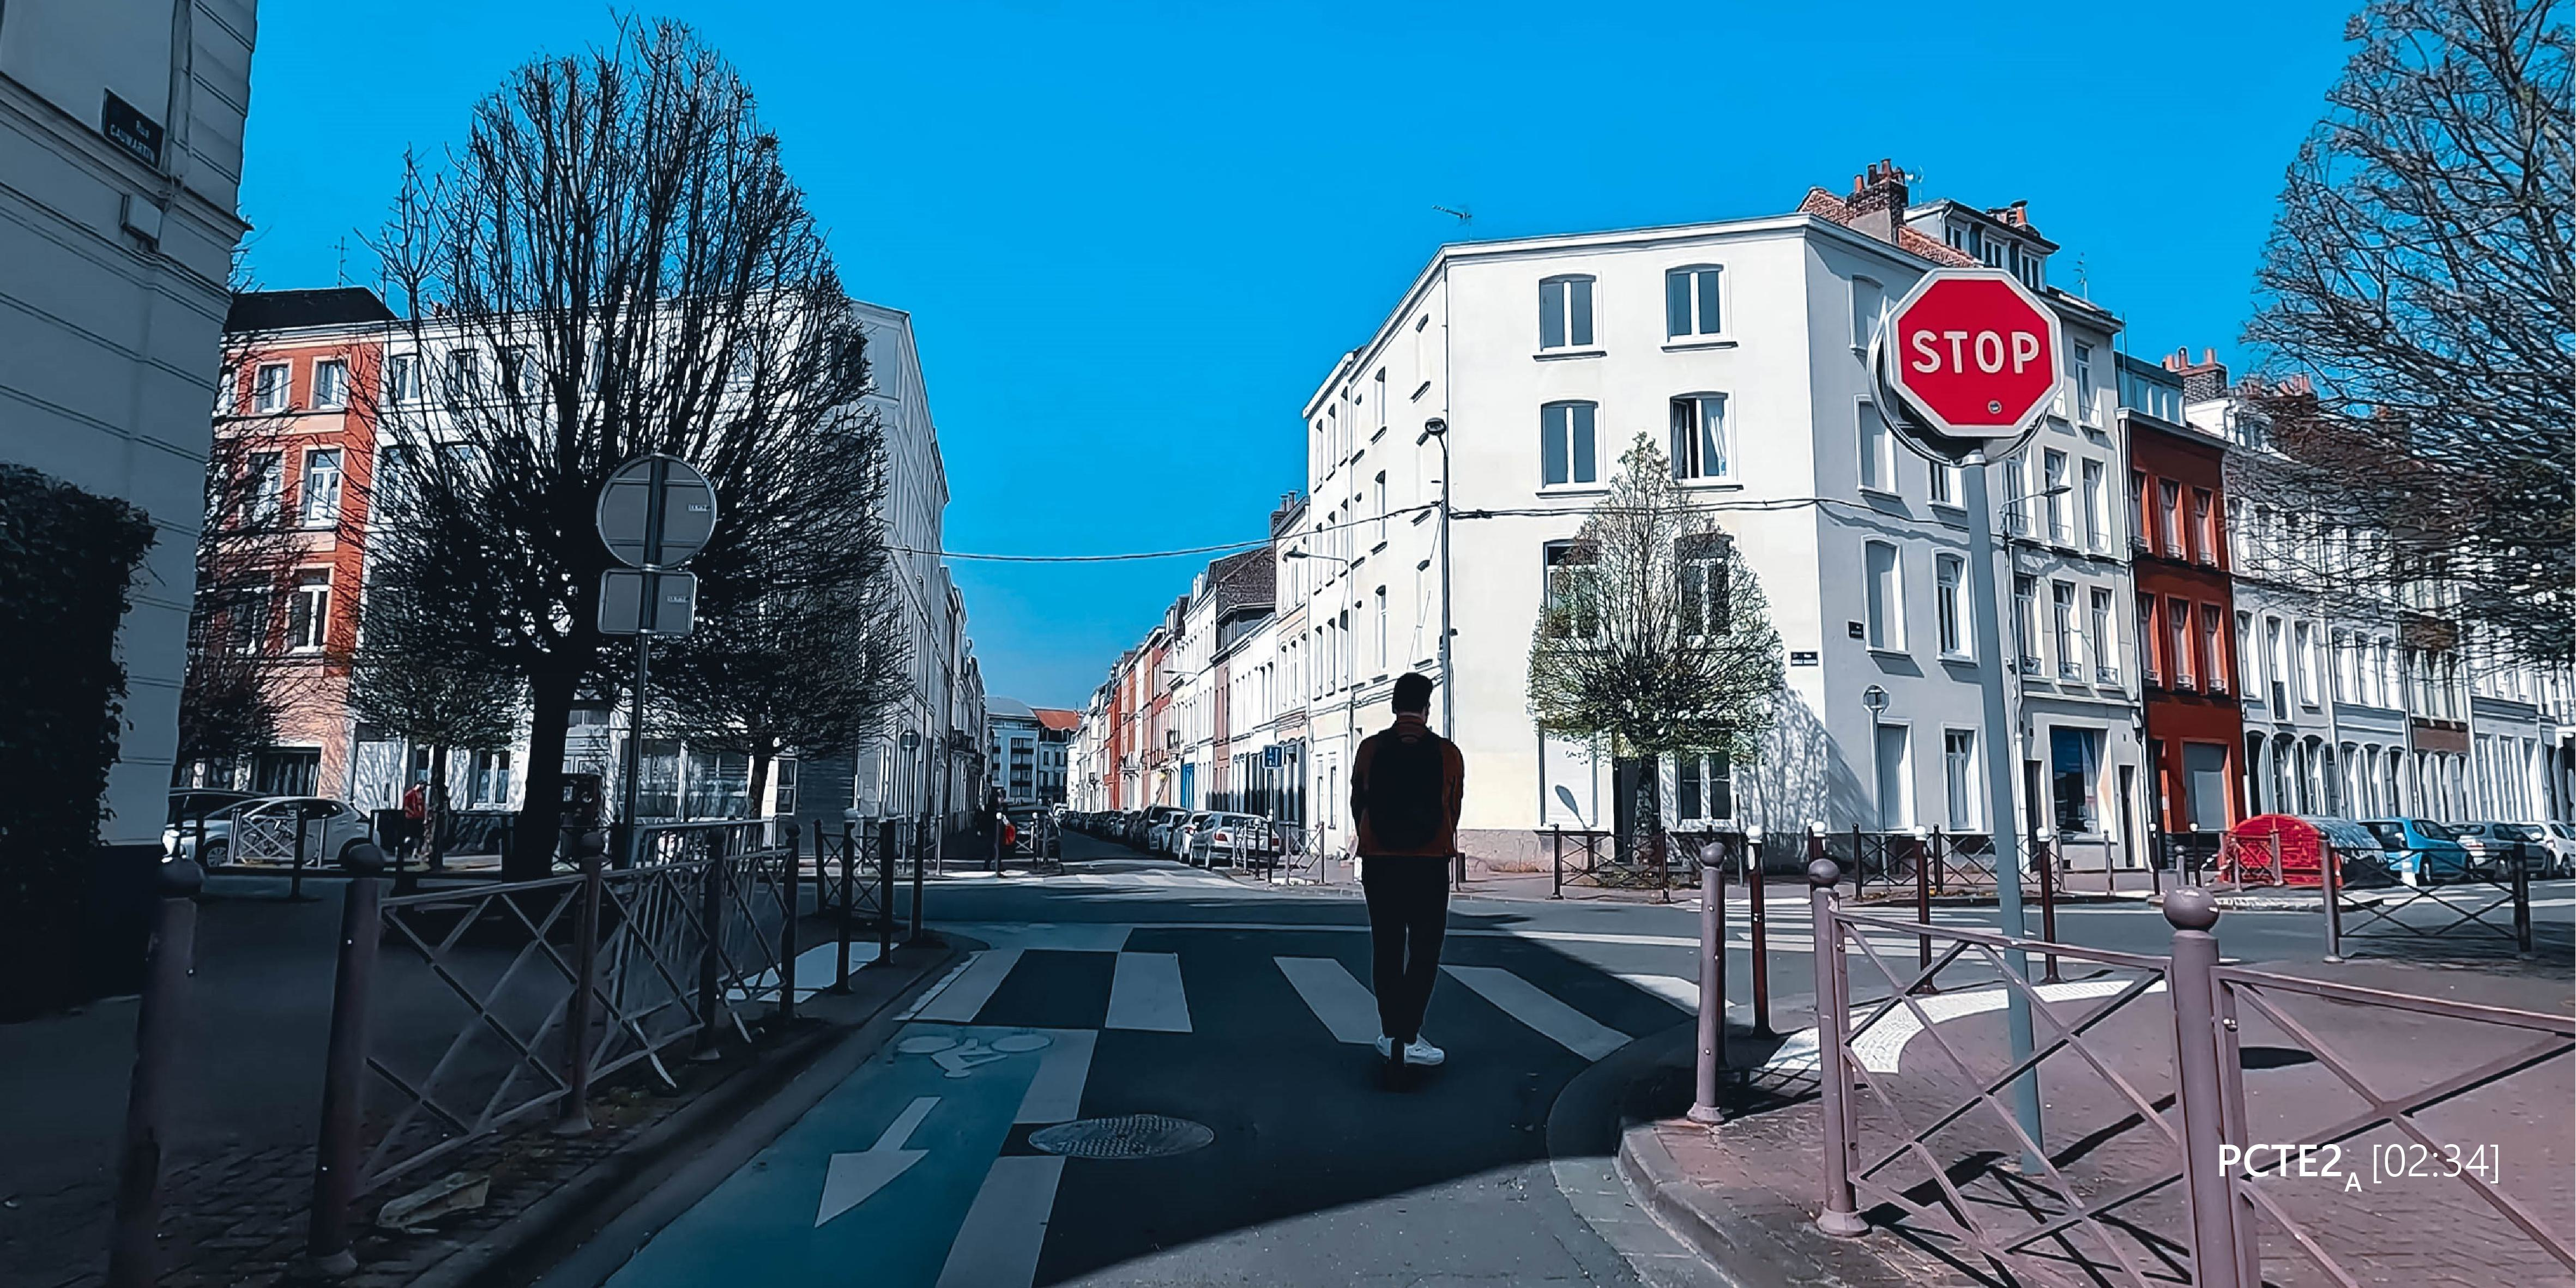
\includegraphics[width=0.75\columnwidth]{src/Figures/Annexes/Extrait_Video_PCTE2_Access_4.jpg}}
        \vspace{5pt}
        \begin{flushright}\scriptsize{
        Auteur~: \textcolor{blue}{Dylan Moinse (2022)}
        }\end{flushright}
    \end{figure}

    % PCTE2 Photo Access 5
    \begin{figure}[h!]\vspace*{4pt}
        \caption*{Extrait n°5 de la vidéo lors du trajet en rabattement (\(PCTE^{A}_{2}\))}
        \centerline{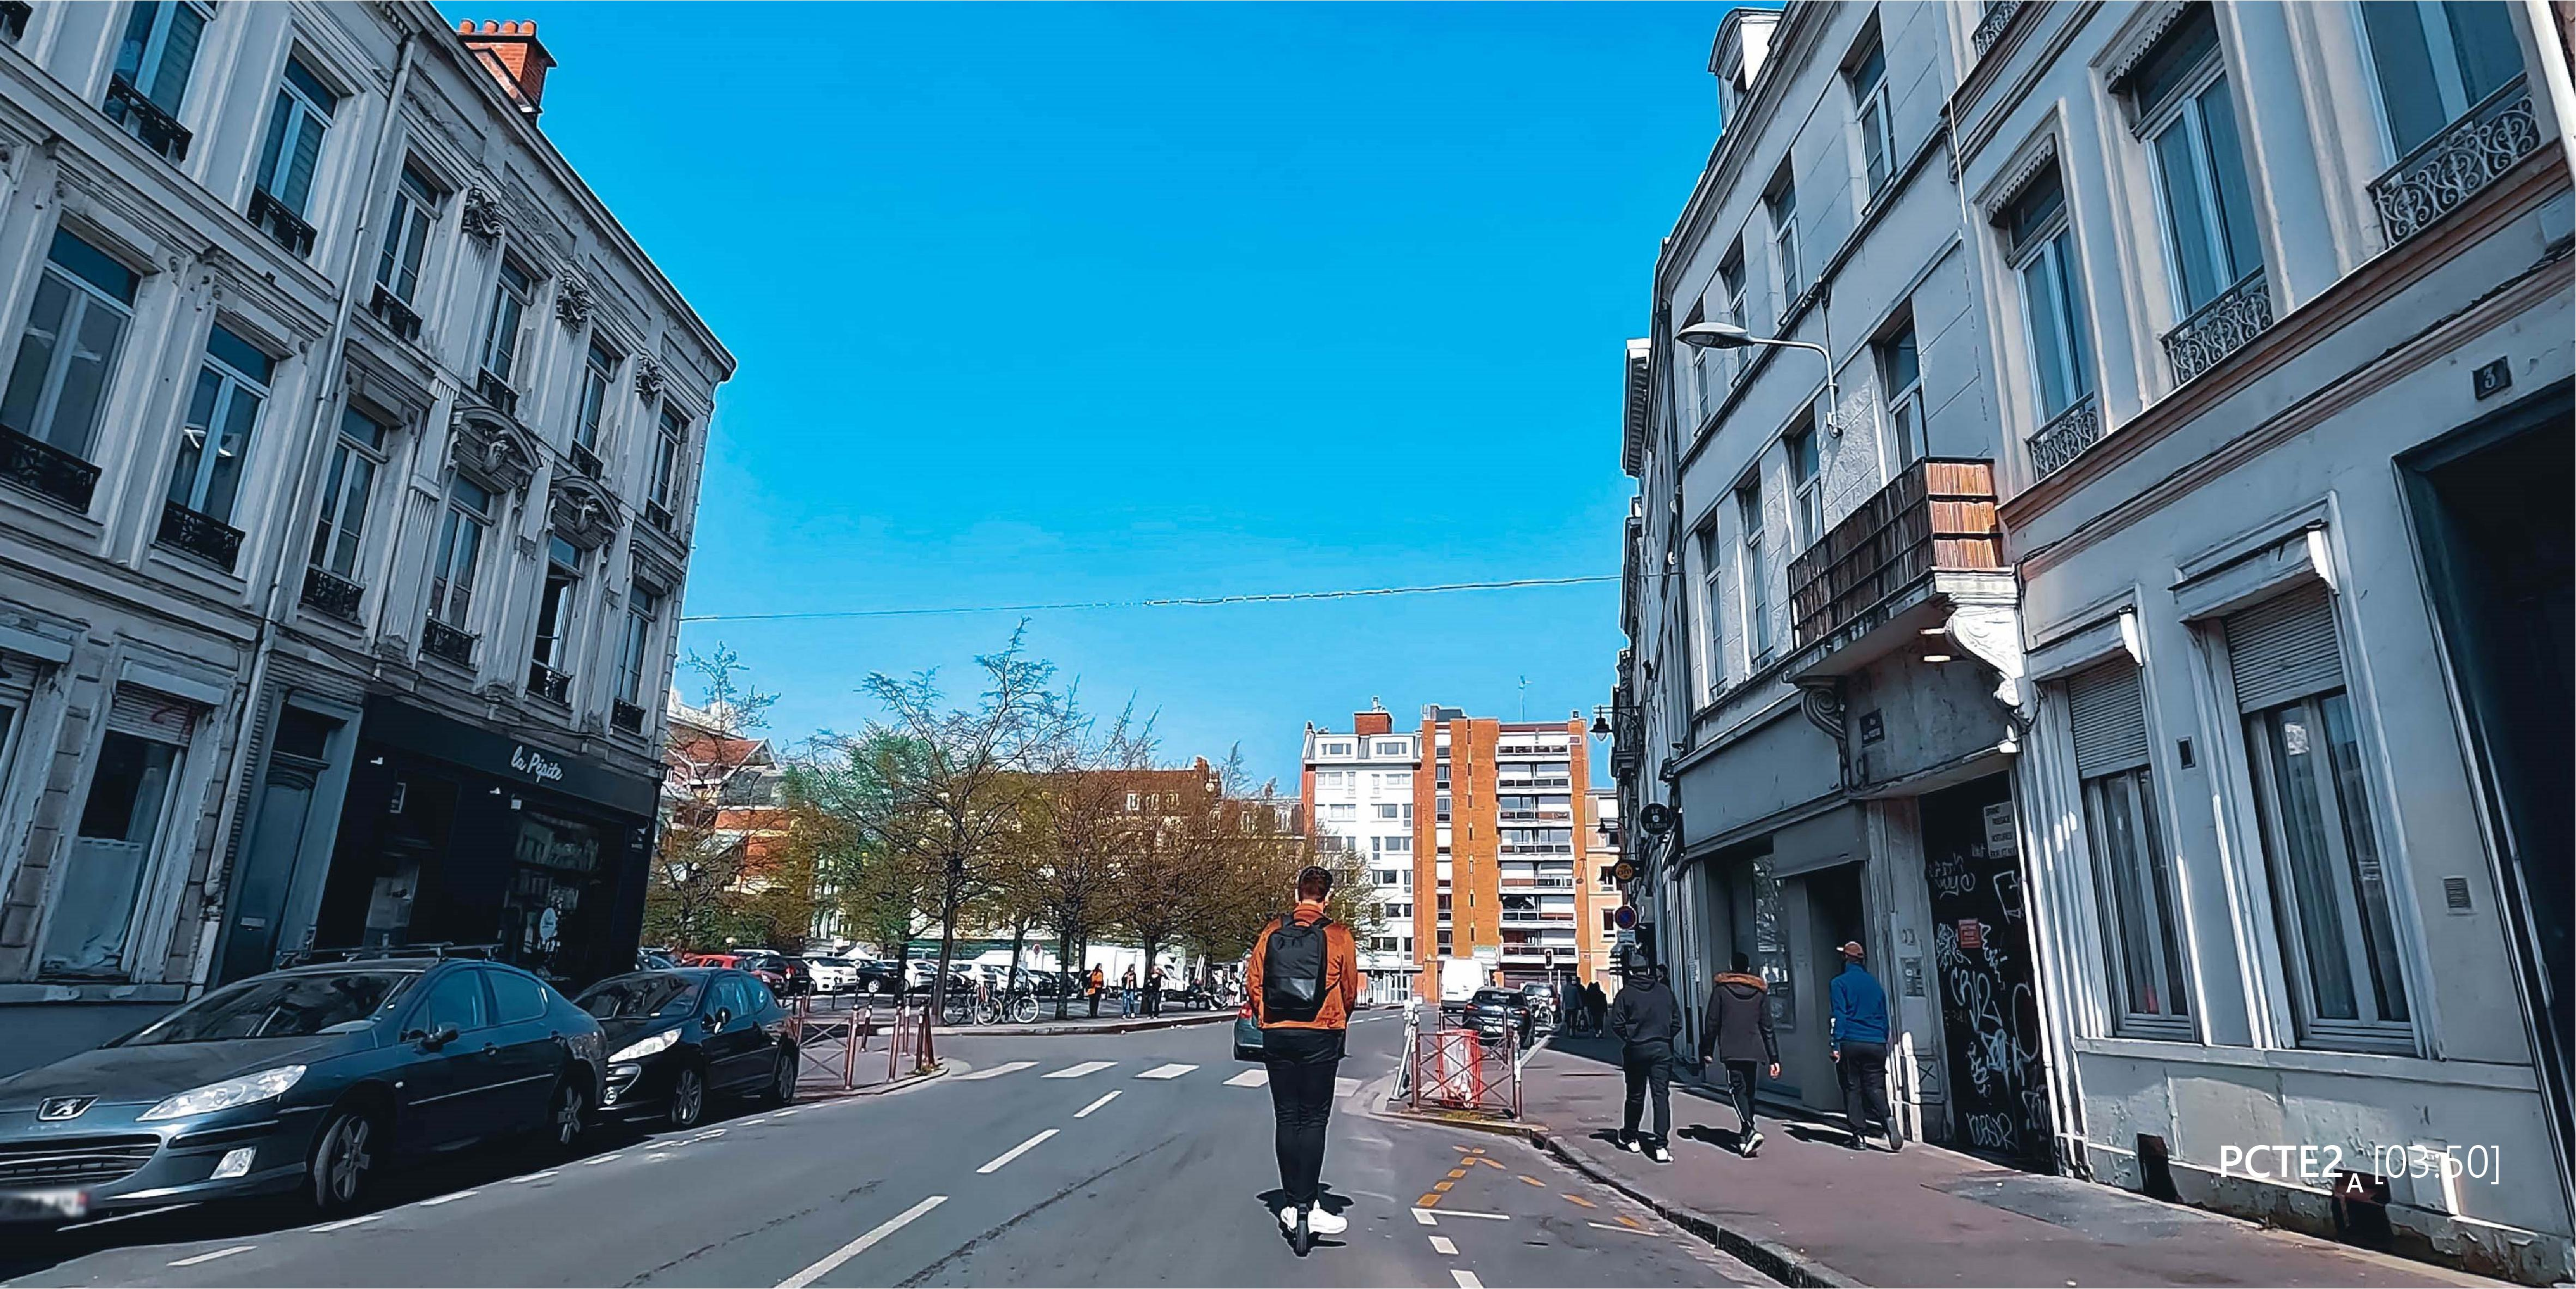
\includegraphics[width=0.75\columnwidth]{src/Figures/Annexes/Extrait_Video_PCTE2_Access_5.jpg}}
        \vspace{5pt}
        \begin{flushright}\scriptsize{
        Auteur~: \textcolor{blue}{Dylan Moinse (2022)}
        }\end{flushright}
    \end{figure}

    % PCTE2 Photo Access 6
    \begin{figure}[h!]\vspace*{4pt}
        \caption*{Extrait n°6 de la vidéo lors du trajet en rabattement (\(PCTE^{A}_{2}\))}
        \centerline{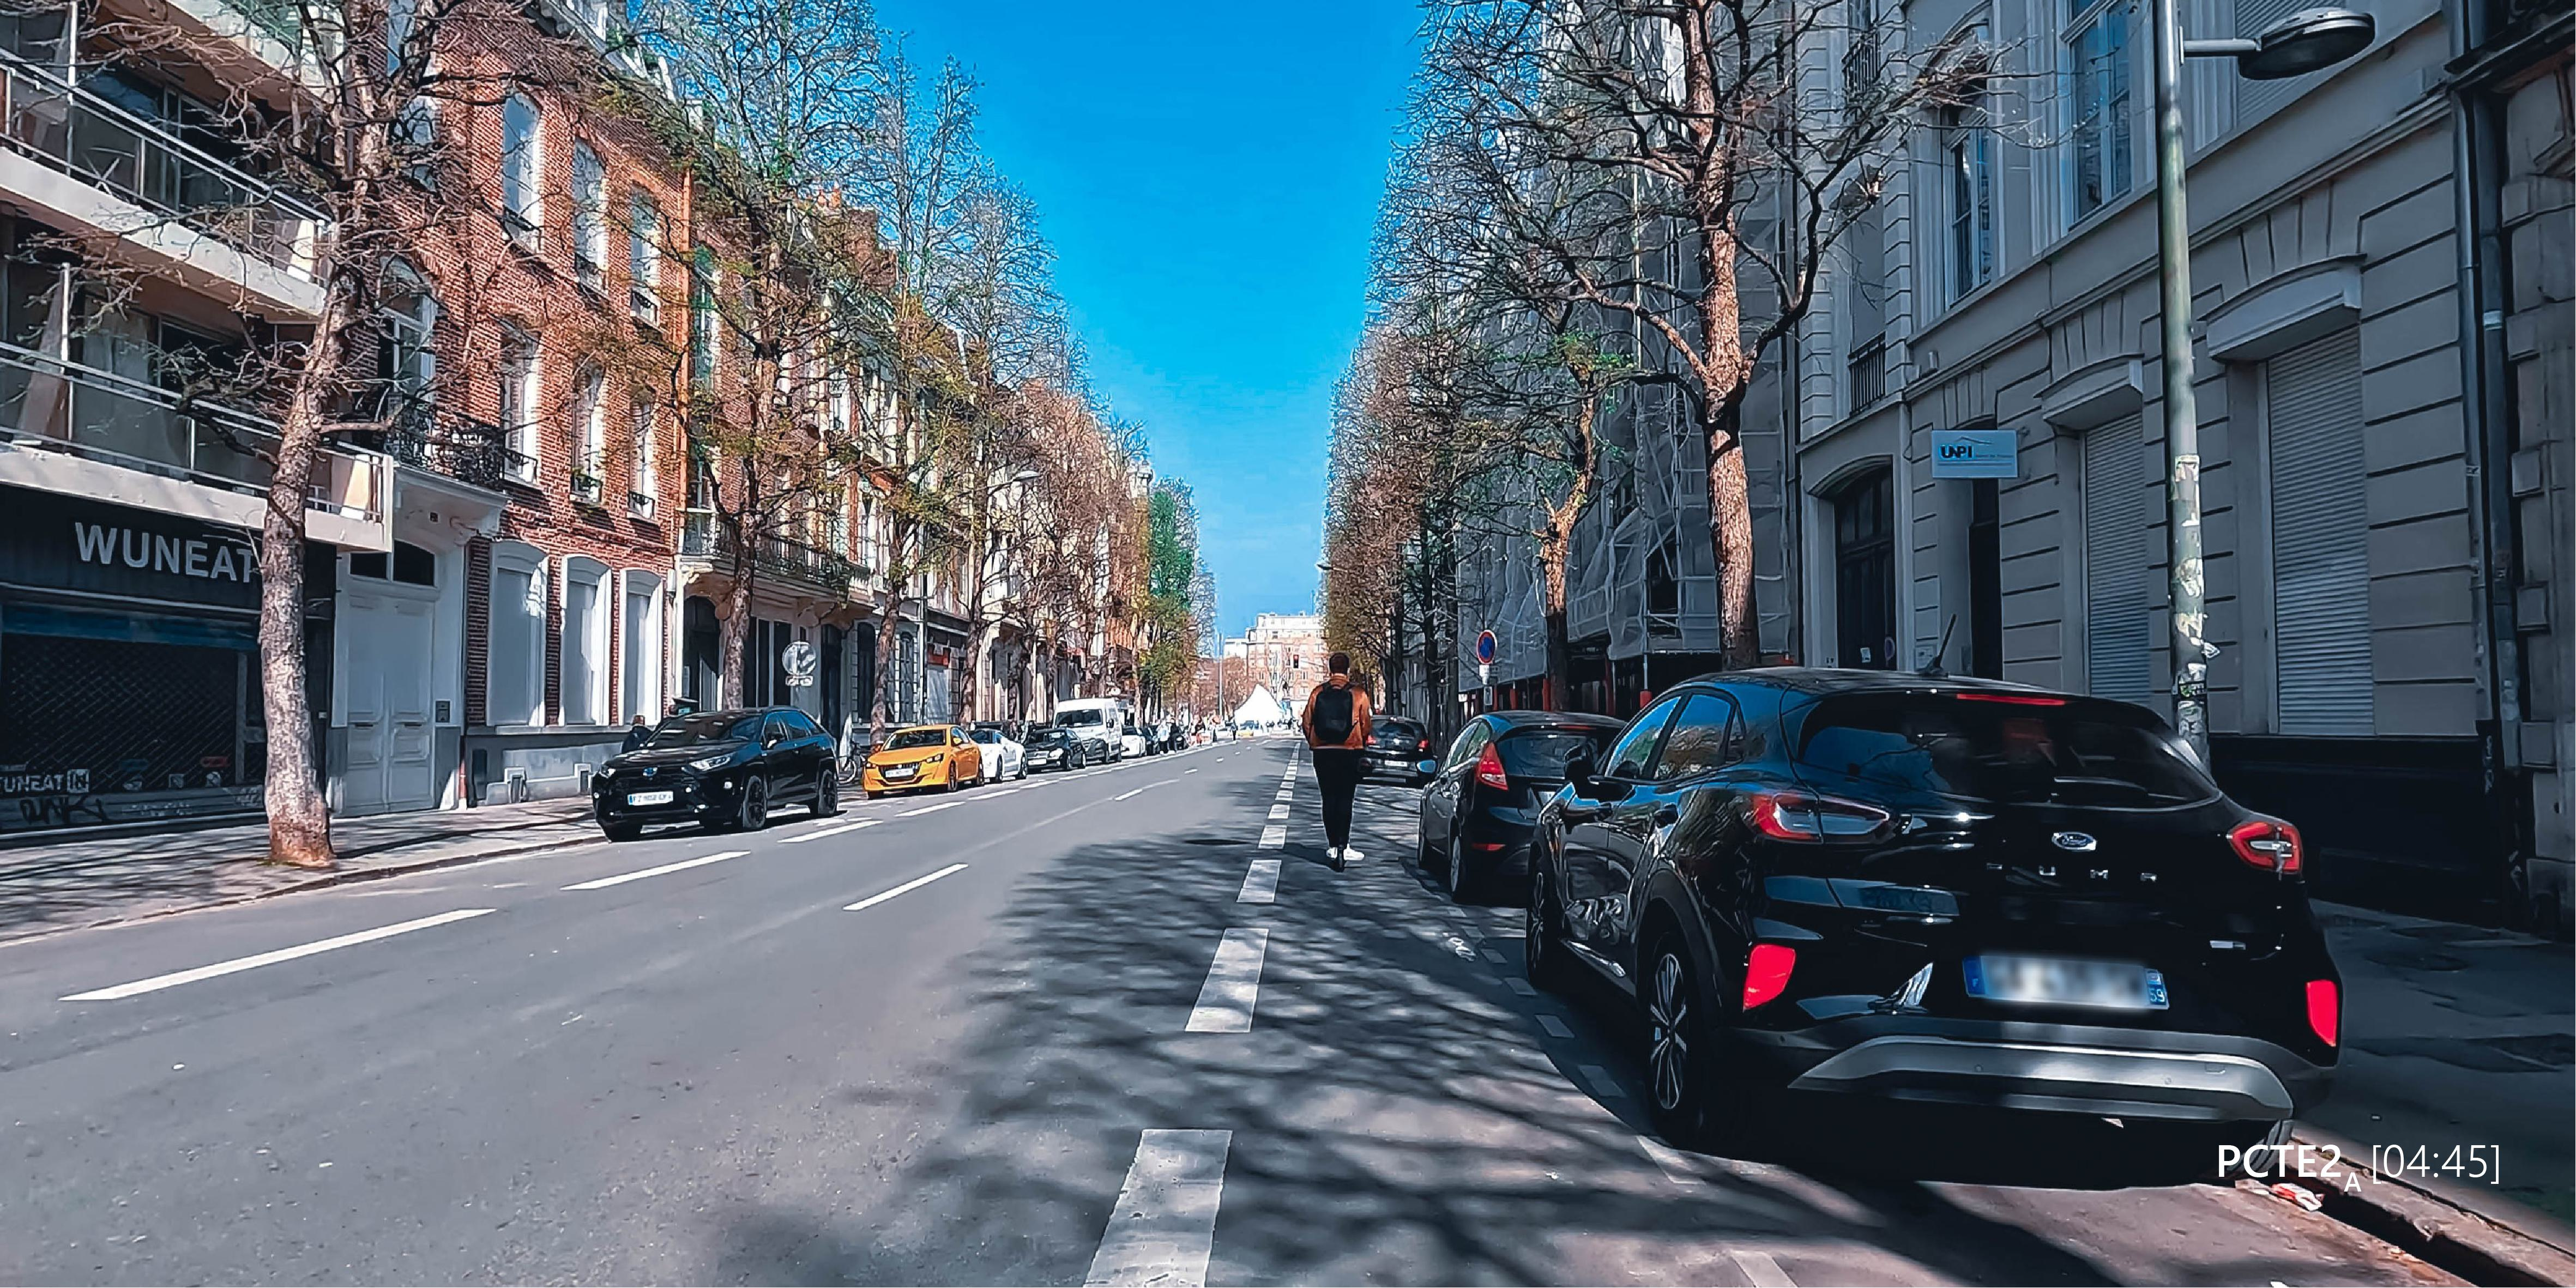
\includegraphics[width=0.75\columnwidth]{src/Figures/Annexes/Extrait_Video_PCTE2_Access_6.jpg}}
        \vspace{5pt}
        \begin{flushright}\scriptsize{
        Auteur~: \textcolor{blue}{Dylan Moinse (2022)}
        }\end{flushright}
    \end{figure}

    % PCTE2 Photo Access 7
    \begin{figure}[h!]\vspace*{4pt}
        \caption*{Extrait n°7 de la vidéo lors du trajet en rabattement (\(PCTE^{A}_{2}\))}
        \centerline{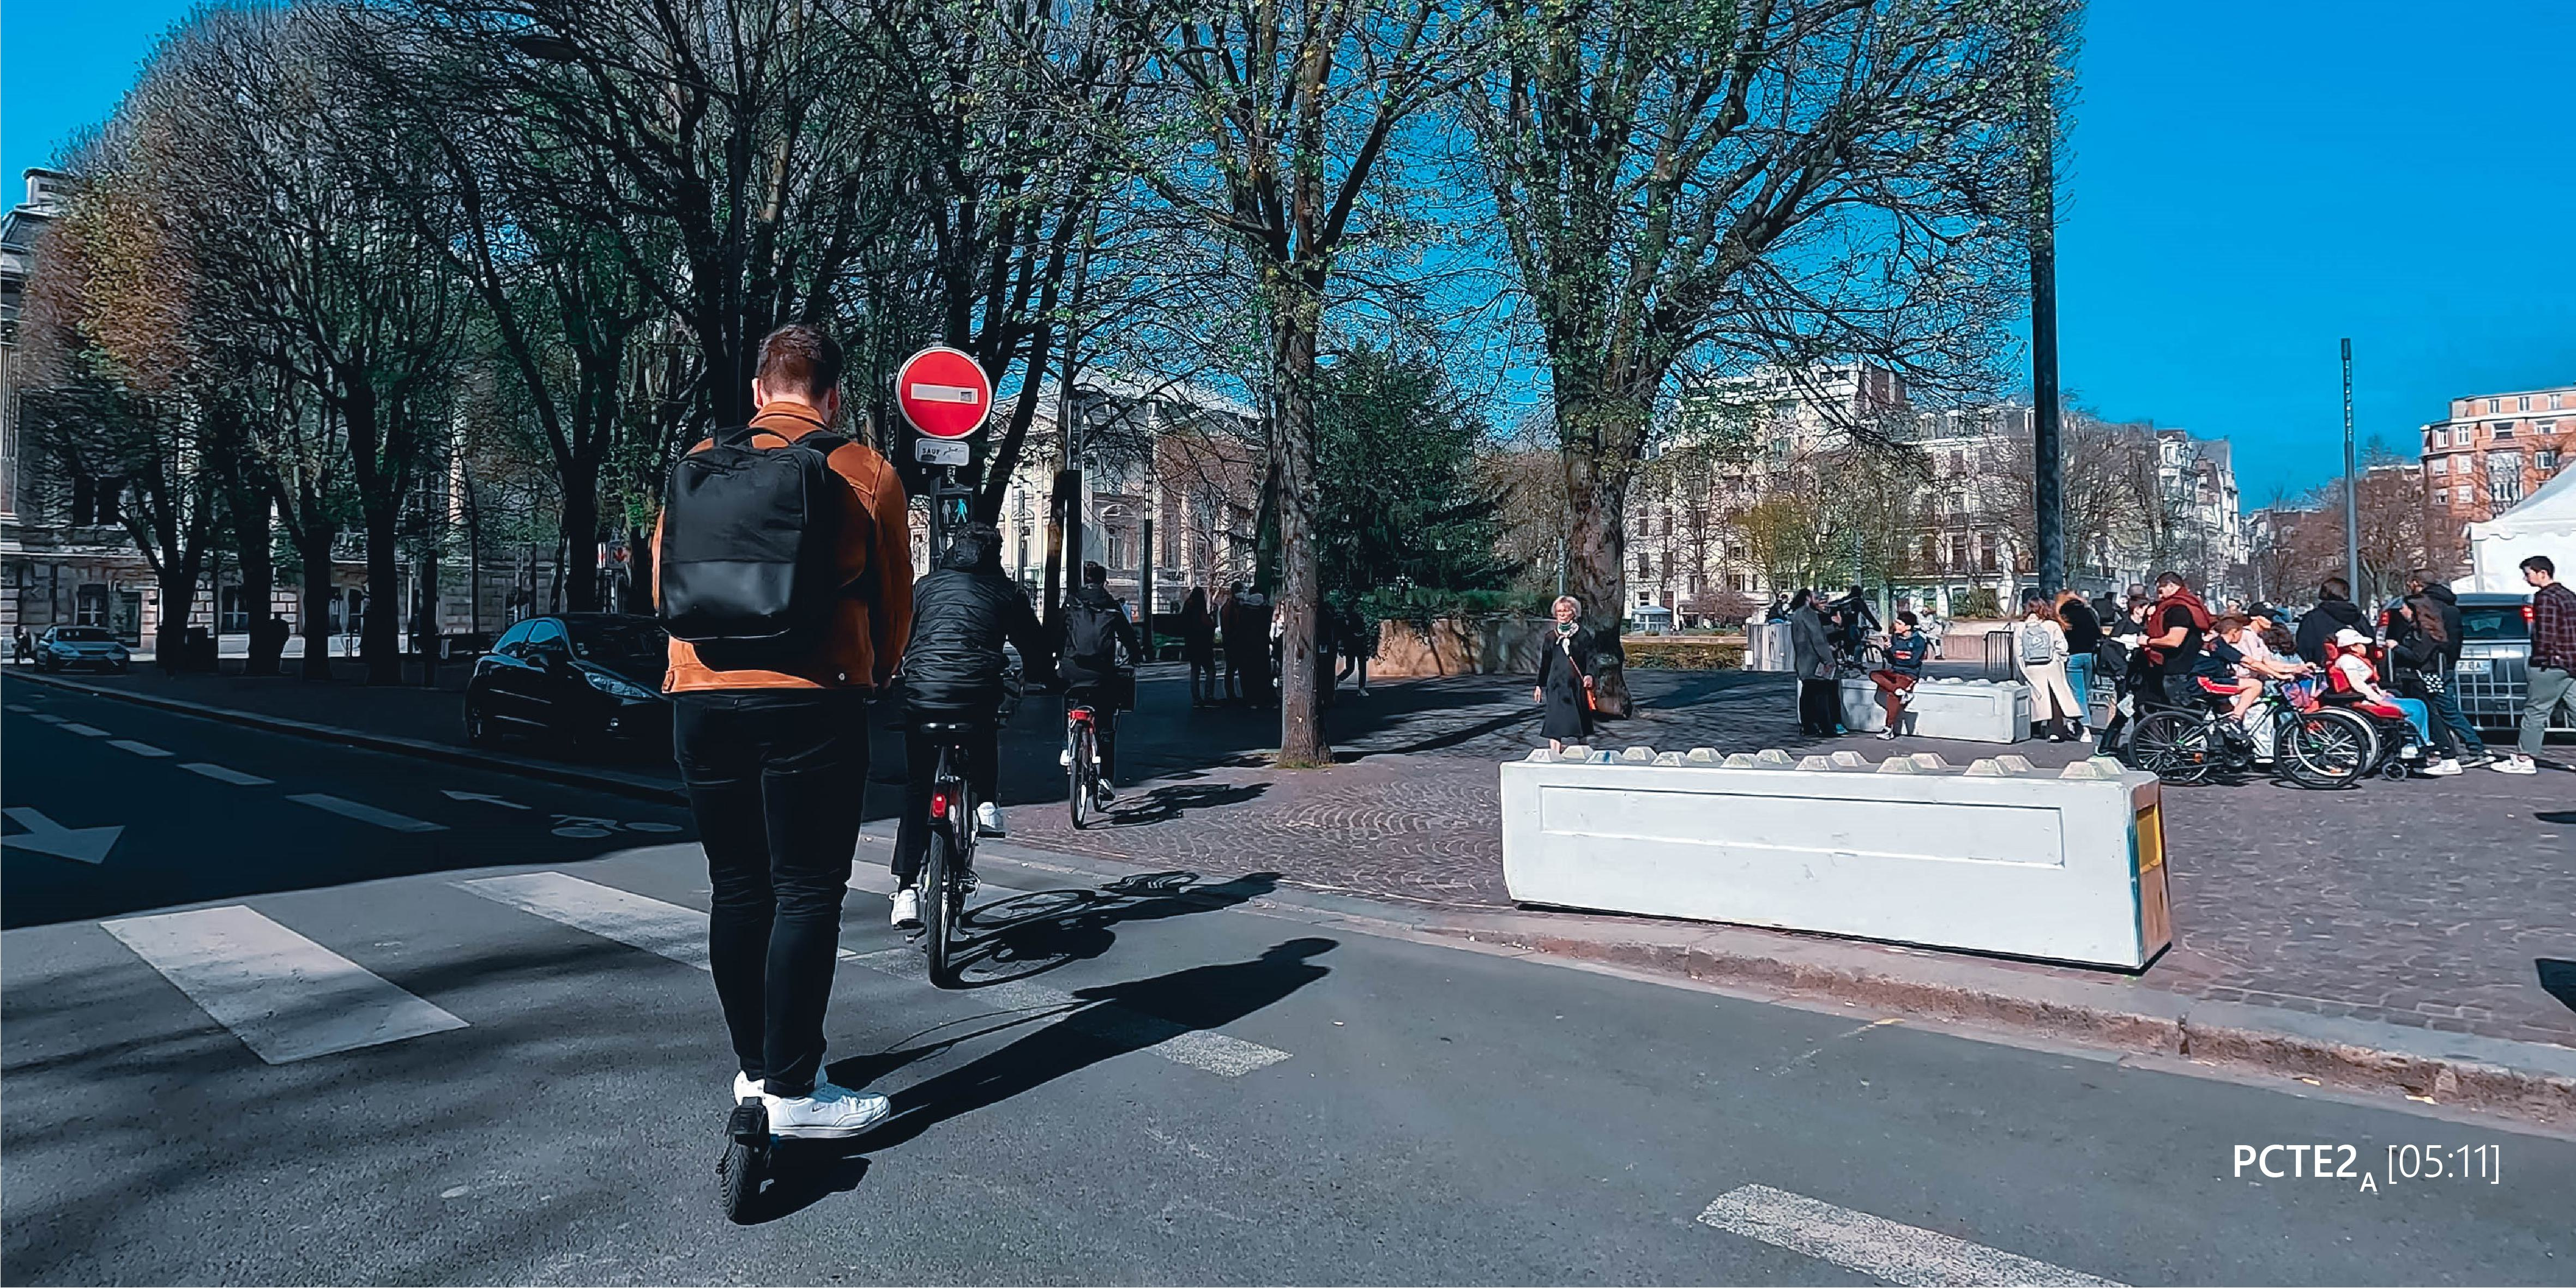
\includegraphics[width=0.75\columnwidth]{src/Figures/Annexes/Extrait_Video_PCTE2_Access_7.jpg}}
        \vspace{5pt}
        \begin{flushright}\scriptsize{
        Auteur~: \textcolor{blue}{Dylan Moinse (2022)}
        }\end{flushright}
    \end{figure}

    % Photos PCTE2 TC
\subsubsection{Sélection d'images extraites lors du trajet en métro}

    % PCTE2 Photo TC 1
    \begin{figure}[h!]\vspace*{4pt}
        \caption*{Extrait n°1 de la vidéo lors du trajet en TER (\(PCTE^{TC}_{2}\))}
        \centerline{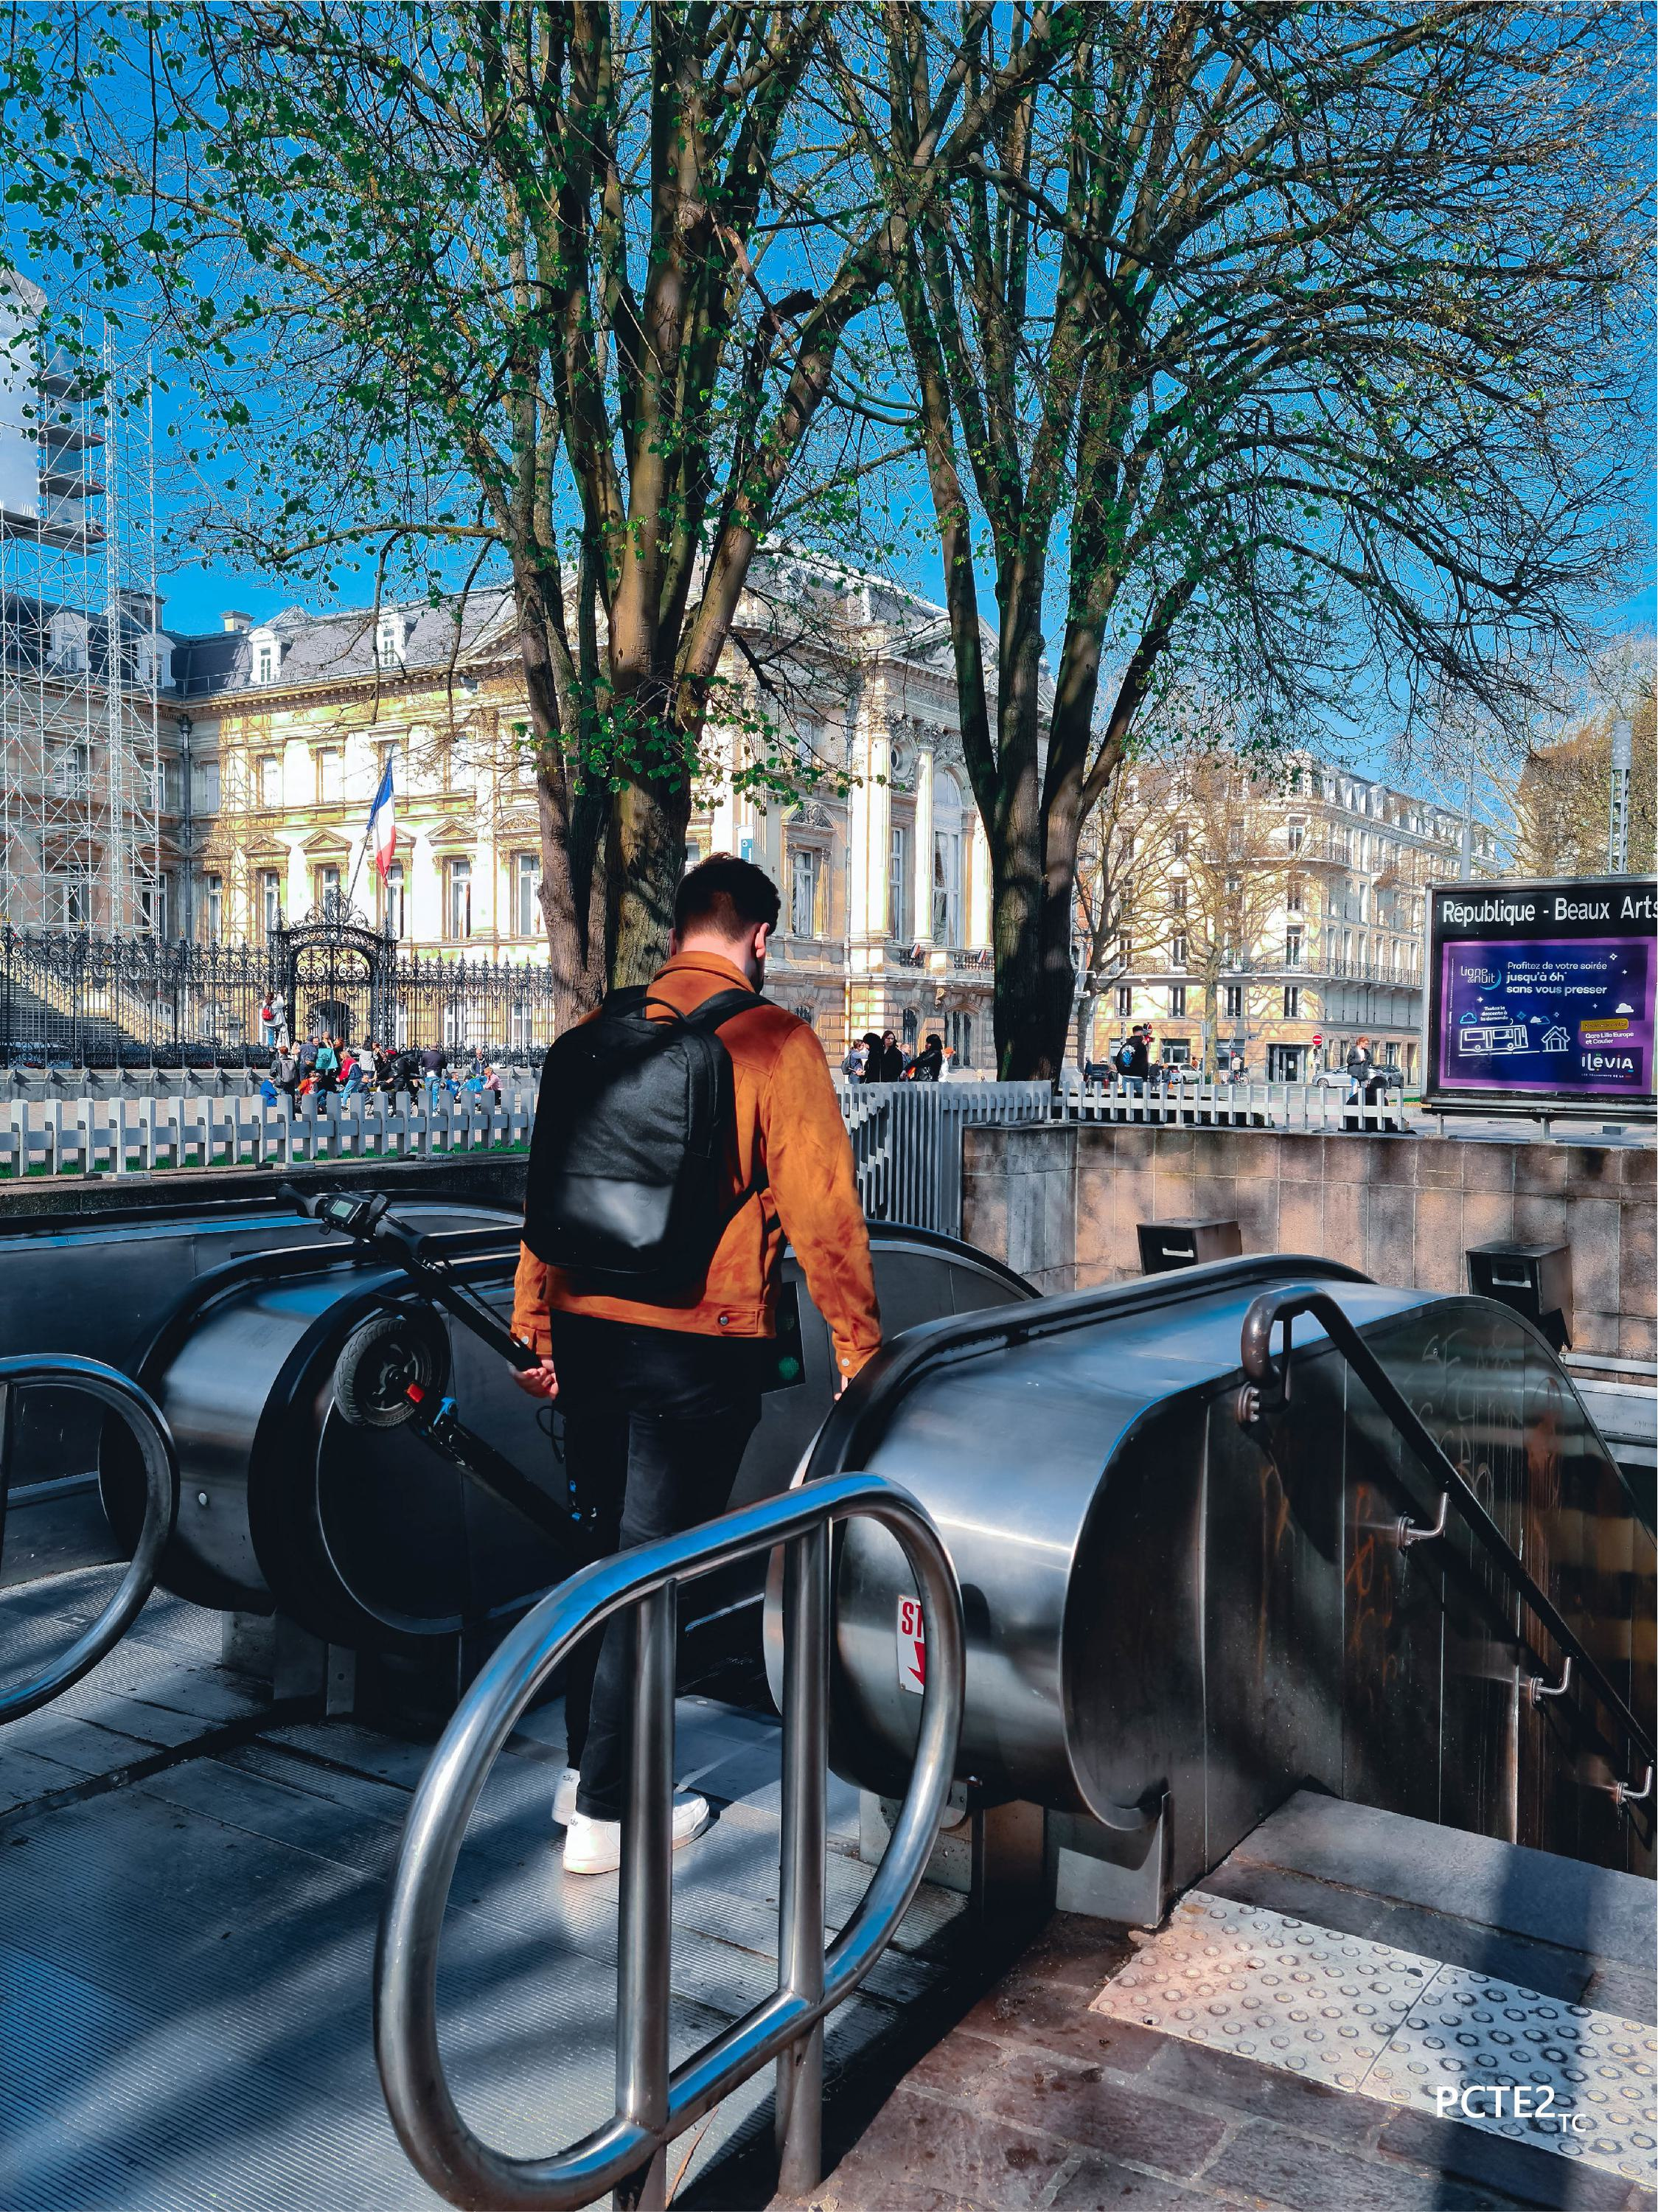
\includegraphics[width=0.5\columnwidth]{src/Figures/Annexes/Extrait_Video_PCTE2_TC_1.jpg}}
        \vspace{5pt}
        \begin{flushright}\scriptsize{
        Auteur~: \textcolor{blue}{Dylan Moinse (2022)}
        }\end{flushright}
    \end{figure}

    % PCTE2 Photo TC 2
    \begin{figure}[h!]\vspace*{4pt}
        \caption*{Extrait n°2 de la vidéo lors du trajet en TER (\(PCTE^{TC}_{2}\))}
        \centerline{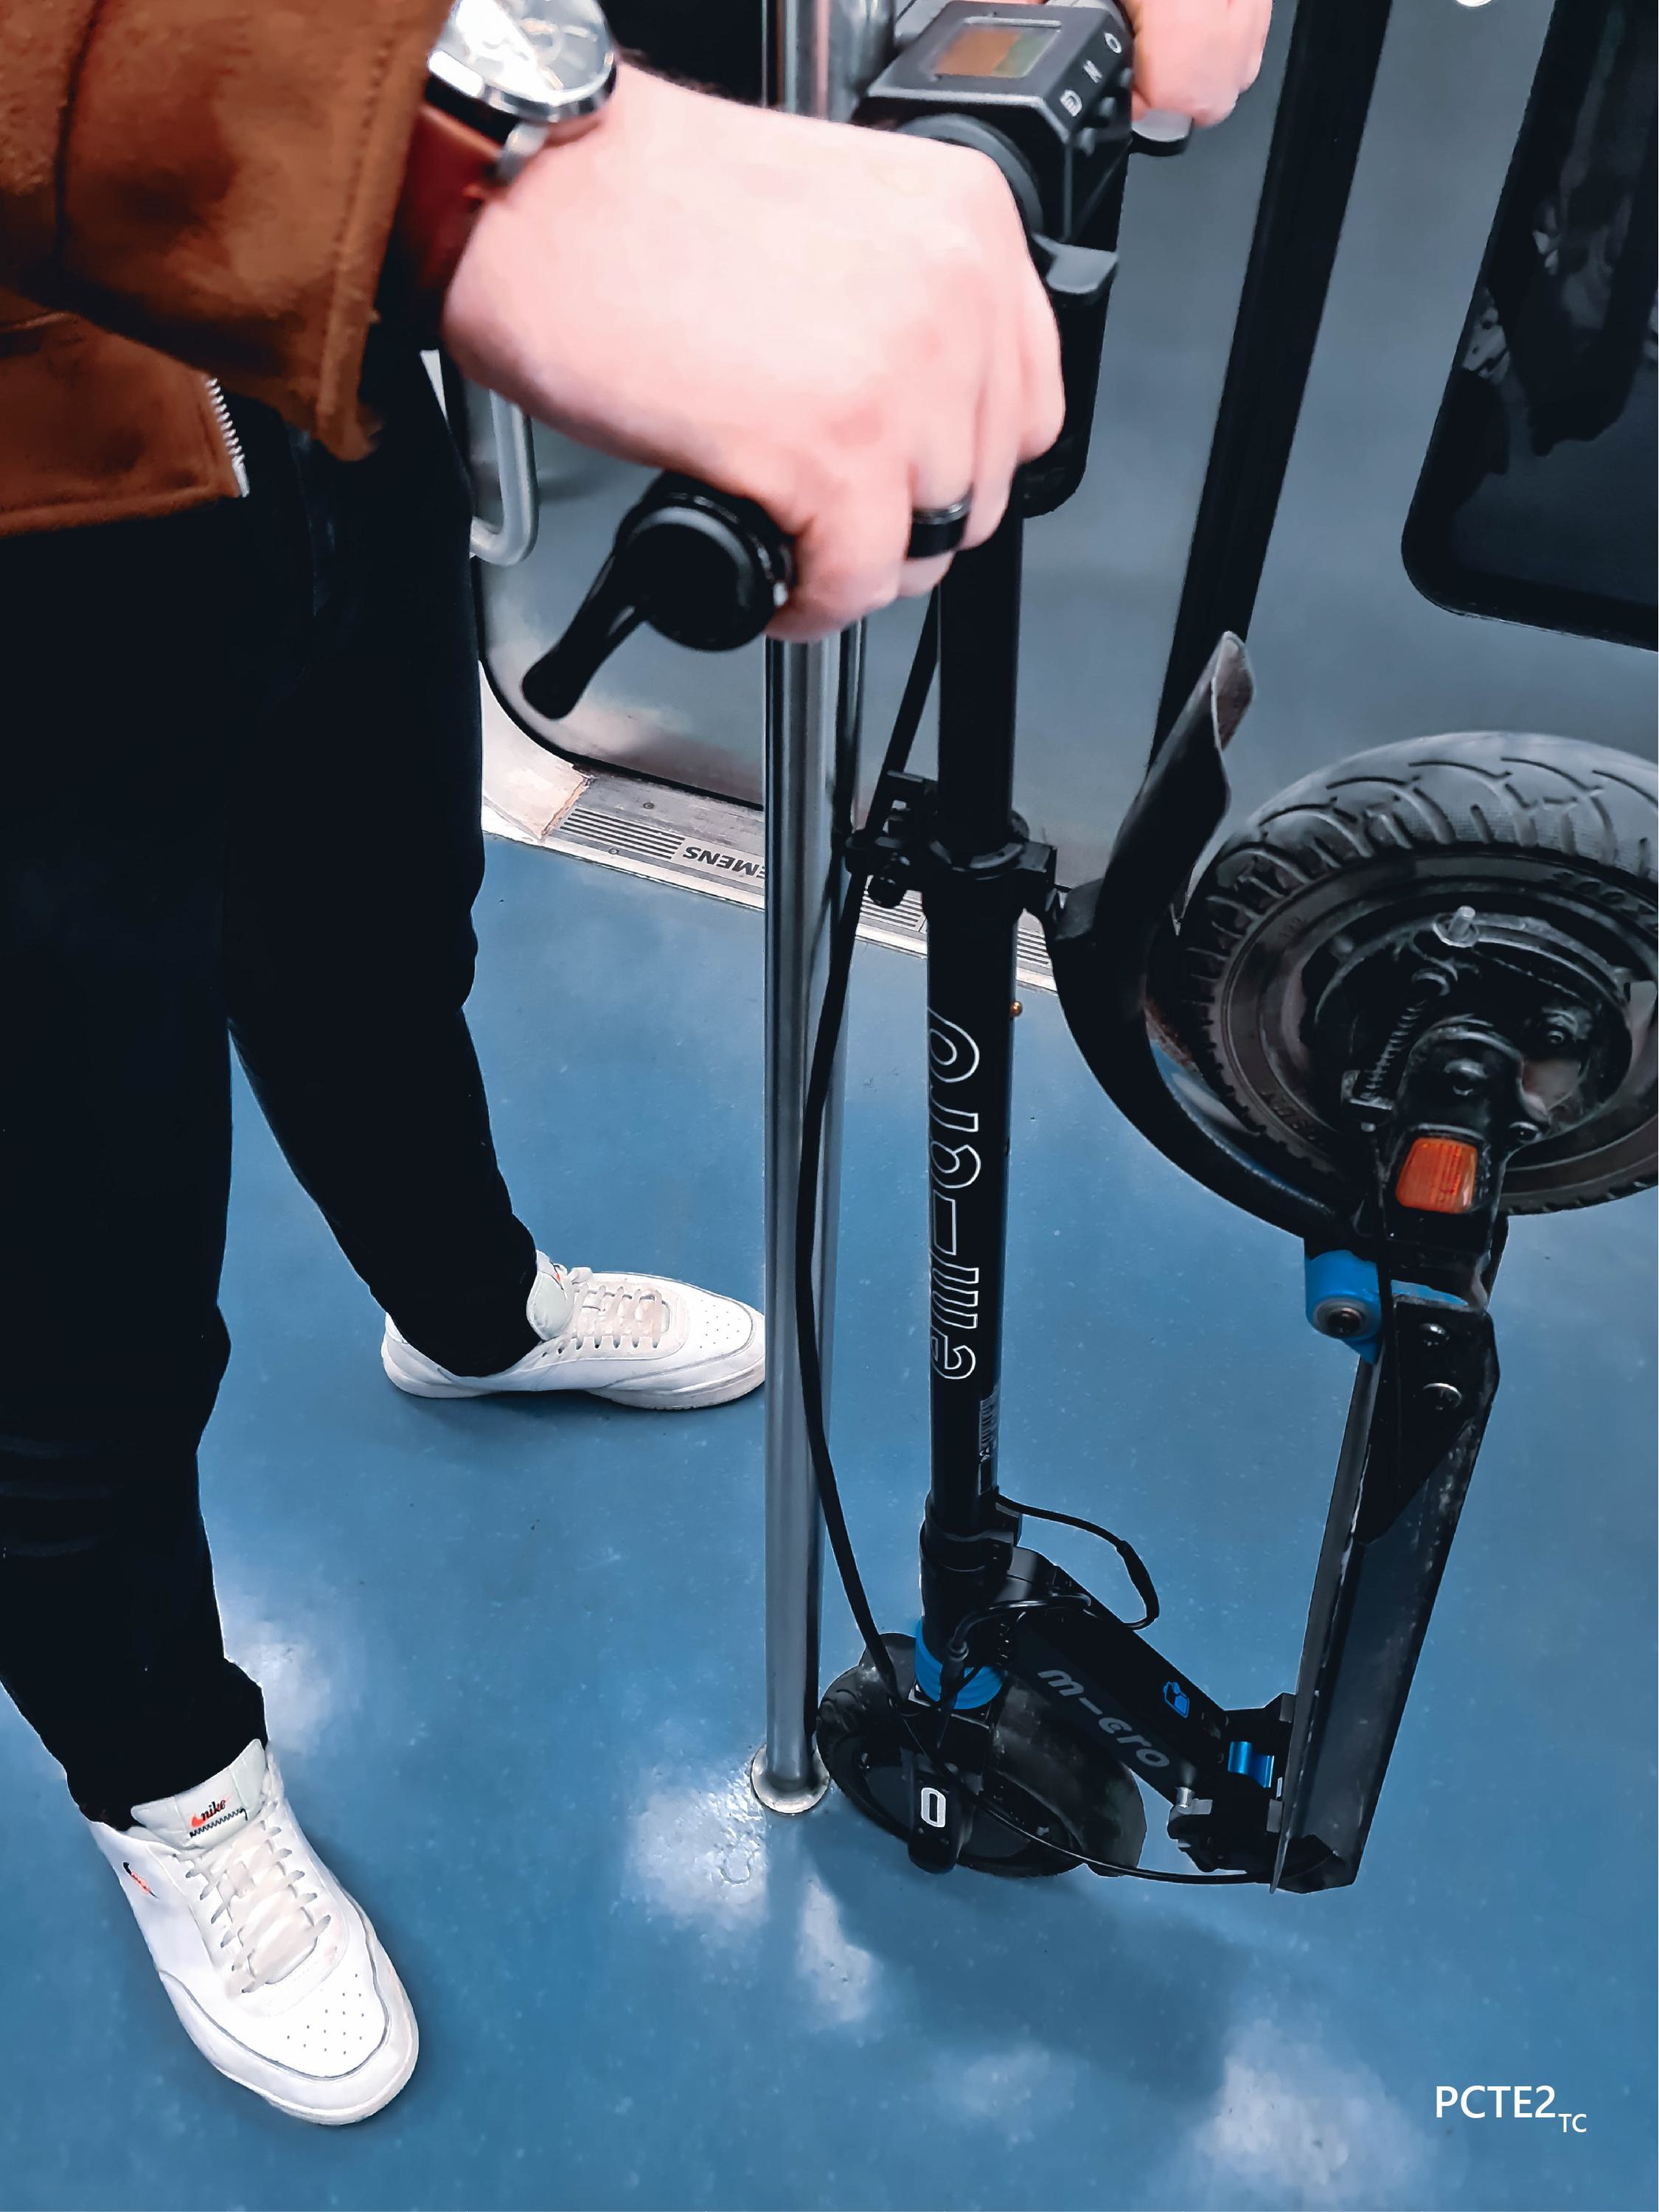
\includegraphics[width=0.5\columnwidth]{src/Figures/Annexes/Extrait_Video_PCTE2_TC_2.jpg}}
        \vspace{5pt}
        \begin{flushright}\scriptsize{
        Auteur~: \textcolor{blue}{Dylan Moinse (2022)}
        }\end{flushright}
    \end{figure}
    
    % PCTE2 Photo TC 3
    \begin{figure}[h!]\vspace*{4pt}
        \caption*{Extrait n°3 de la vidéo lors du trajet en TER (\(PCTE^{TC}_{2}\))}
        \centerline{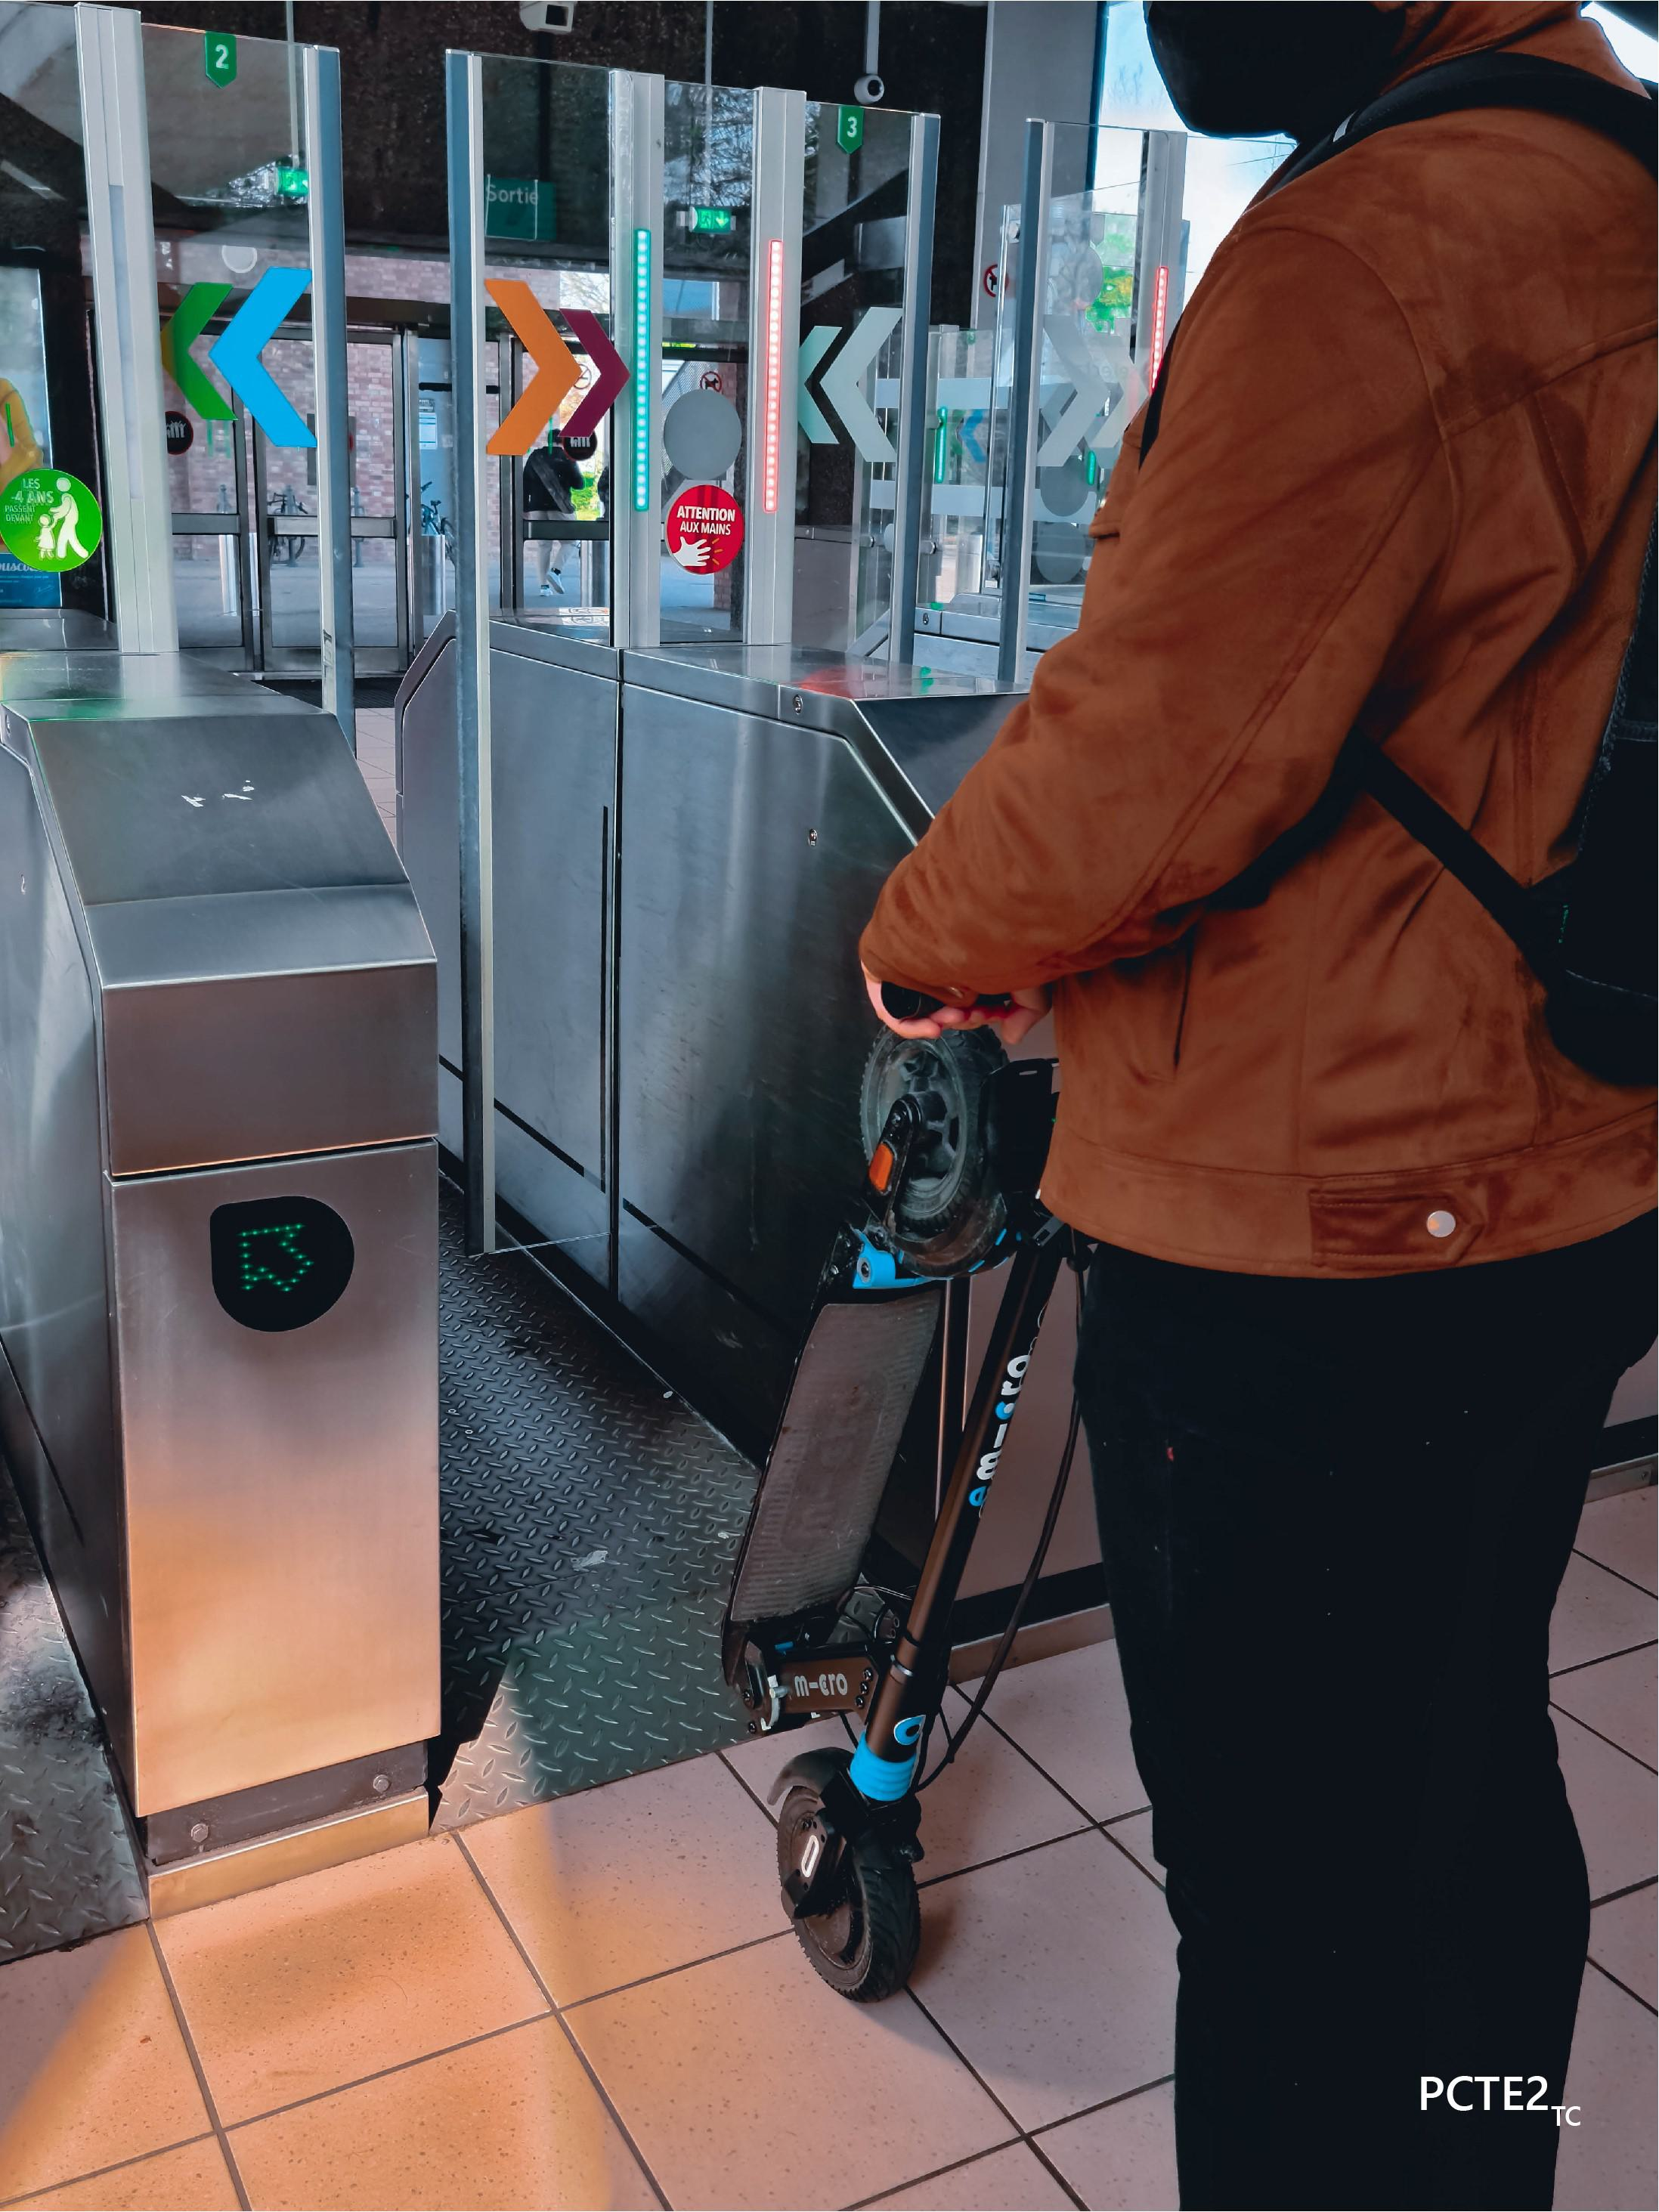
\includegraphics[width=0.5\columnwidth]{src/Figures/Annexes/Extrait_Video_PCTE2_TC_3.jpg}}
        \vspace{5pt}
        \begin{flushright}\scriptsize{
        Auteur~: \textcolor{blue}{Dylan Moinse (2022)}
        }\end{flushright}
    \end{figure}

    % Photos PCTE2 egress
\subsubsection{Sélection d'images extraites lors du trajet en diffusion}

    % PCTE2 Photo Egress 1
    \begin{figure}[h!]\vspace*{4pt}
        \caption*{Extrait n°1 de la vidéo lors du trajet en diffusion (\(PCTE^{E}_{2}\))}
        \centerline{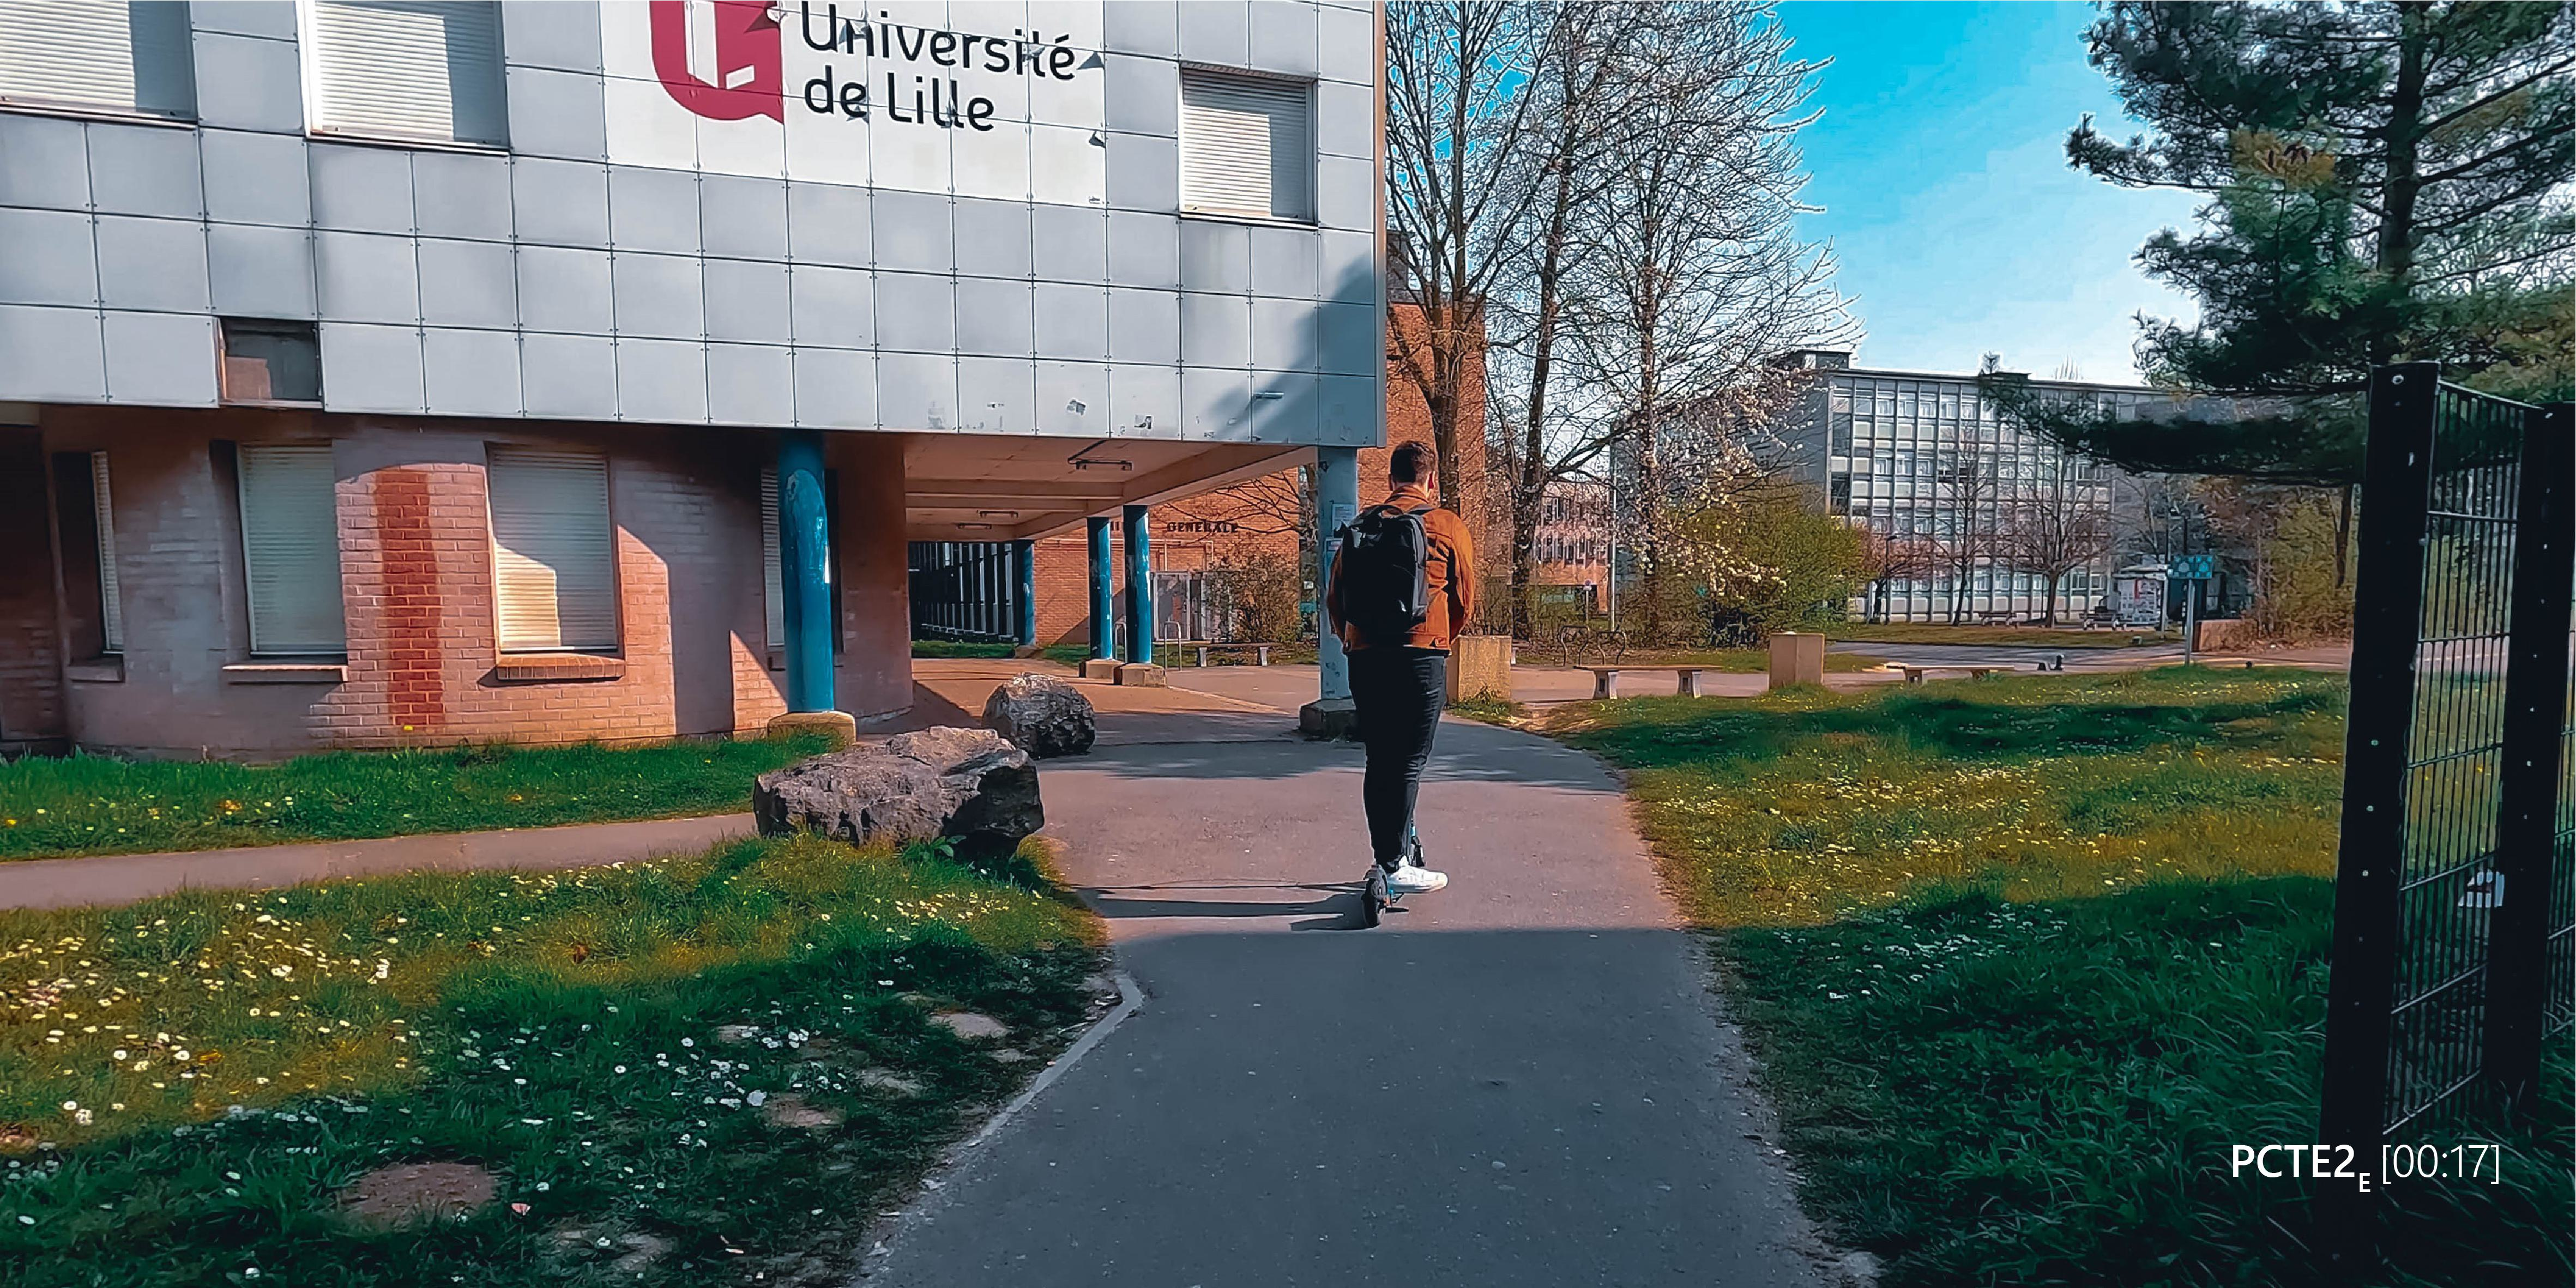
\includegraphics[width=0.75\columnwidth]{src/Figures/Annexes/Extrait_Video_PCTE2_Egress_1.jpg}}
        \vspace{5pt}
        \begin{flushright}\scriptsize{
        Auteur~: \textcolor{blue}{Dylan Moinse (2022)}
        }\end{flushright}
    \end{figure}

    % PCTE2 Photo Egress 2
    \begin{figure}[h!]\vspace*{4pt}
        \caption*{Extrait n°2 de la vidéo lors du trajet en diffusion (\(PCTE^{E}_{2}\))}
        \centerline{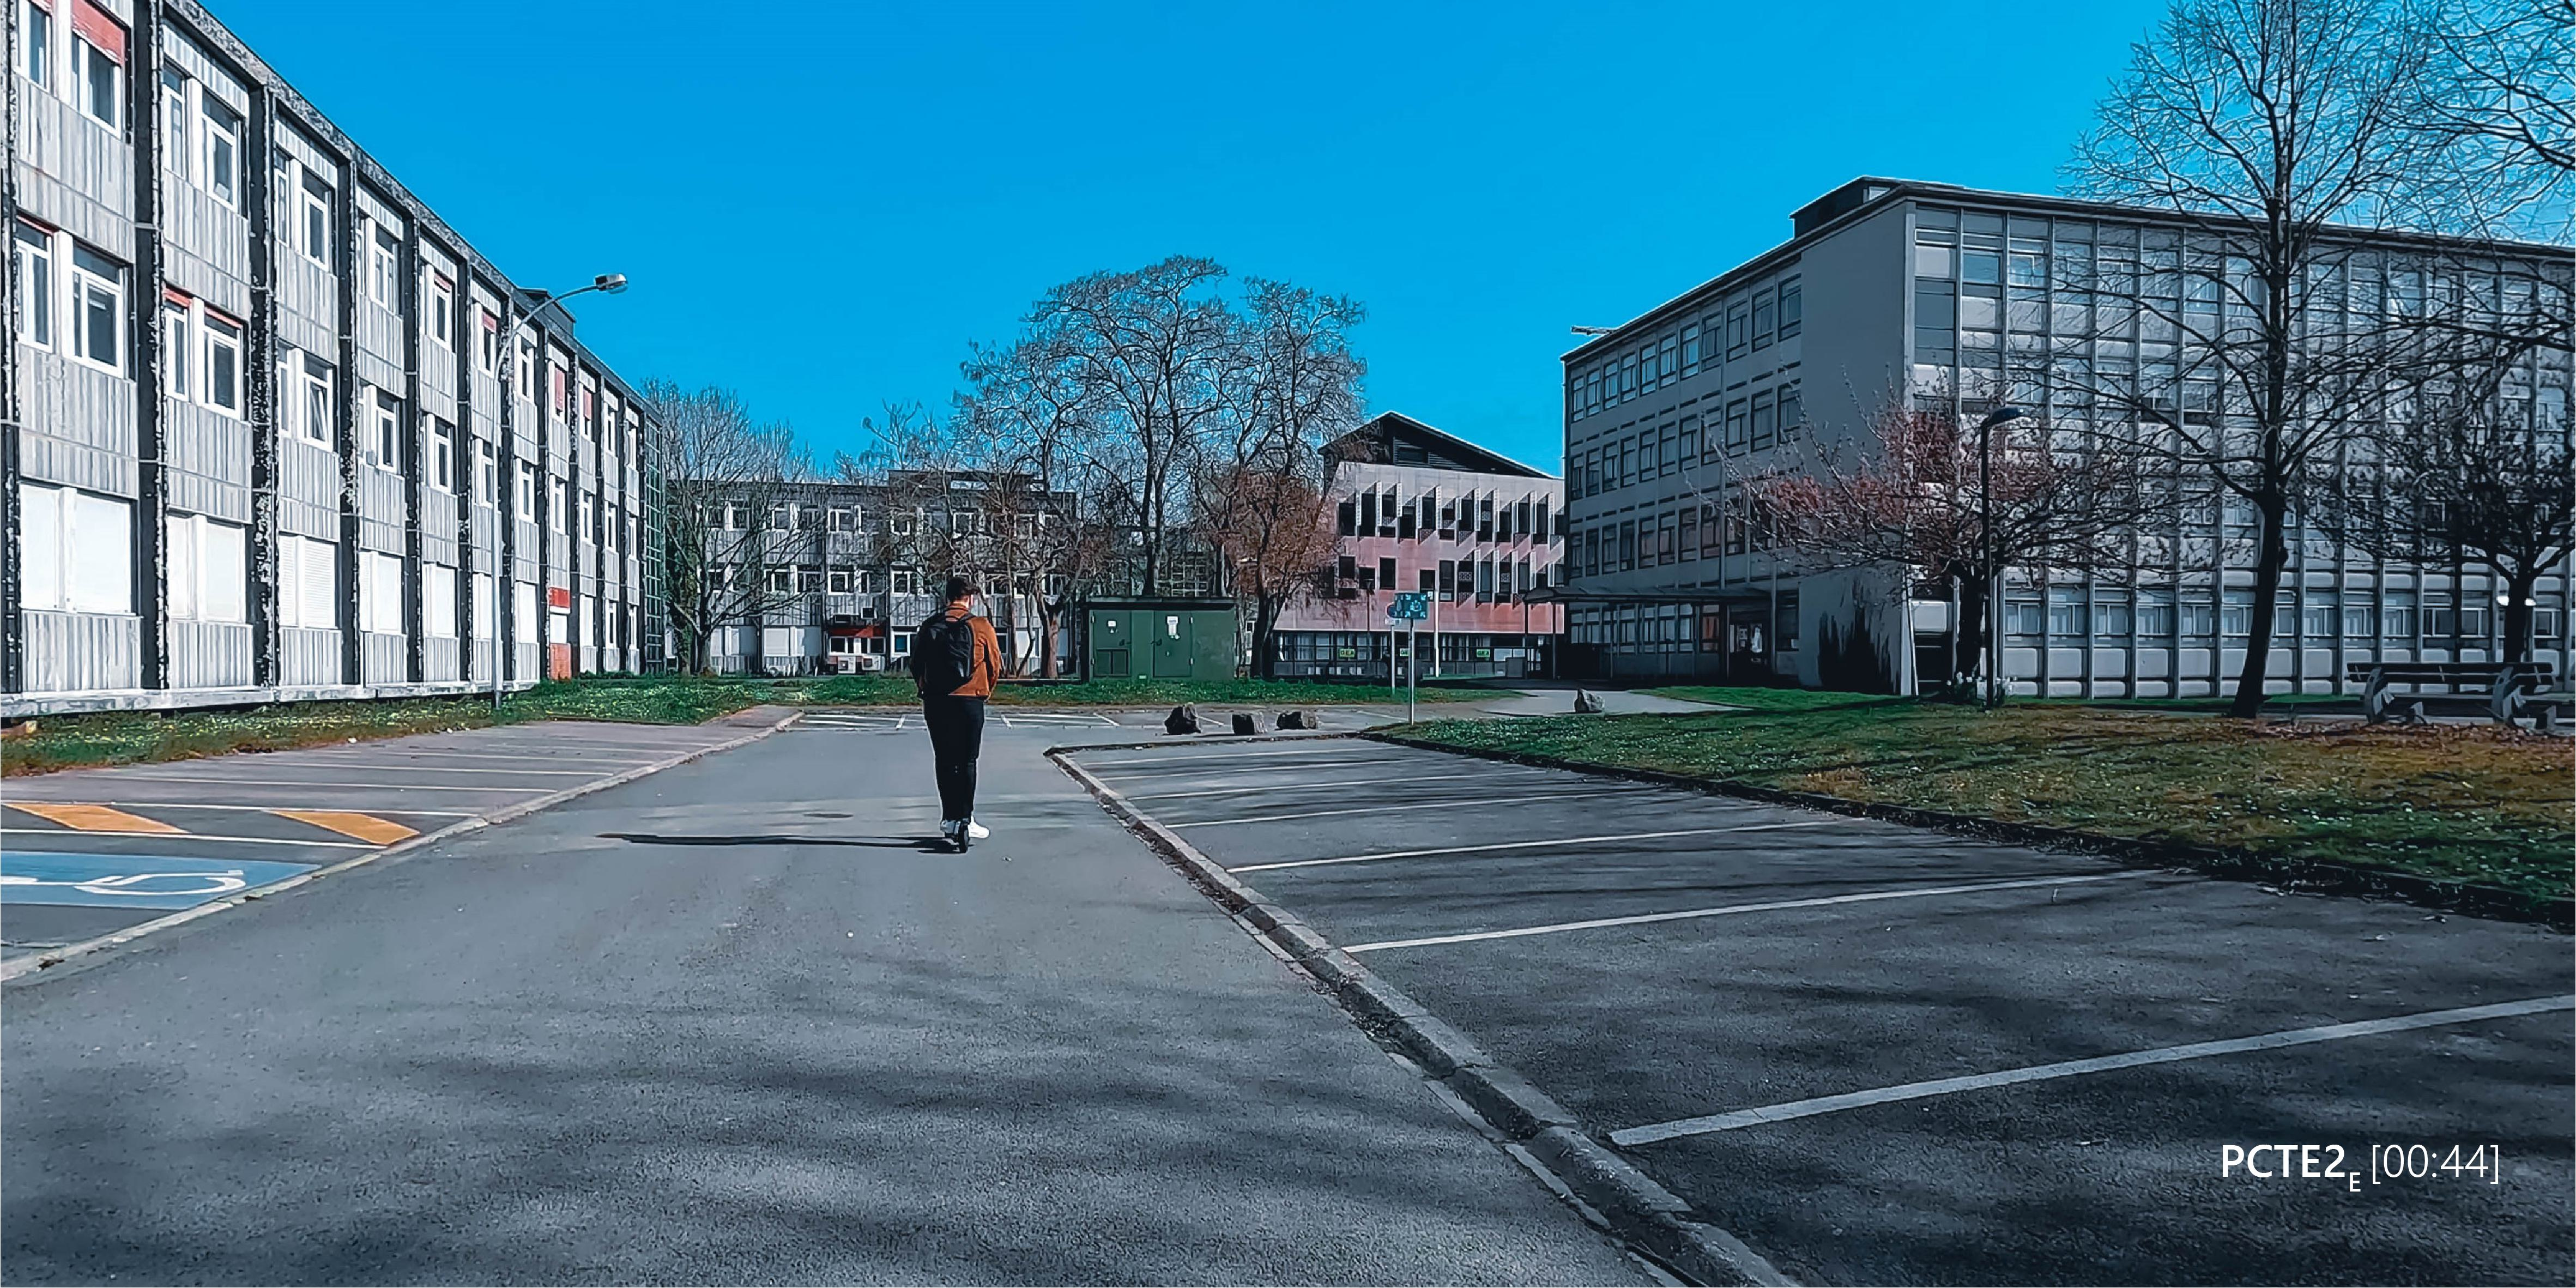
\includegraphics[width=0.75\columnwidth]{src/Figures/Annexes/Extrait_Video_PCTE2_Egress_2.jpg}}
        \vspace{5pt}
        \begin{flushright}\scriptsize{
        Auteur~: \textcolor{blue}{Dylan Moinse (2022)}
        }\end{flushright}
    \end{figure}

    % PCTE2 Photo Egress 3
    \begin{figure}[h!]\vspace*{4pt}
        \caption*{Extrait n°3 de la vidéo lors du trajet en diffusion (\(PCTE^{E}_{2}\))}
        \centerline{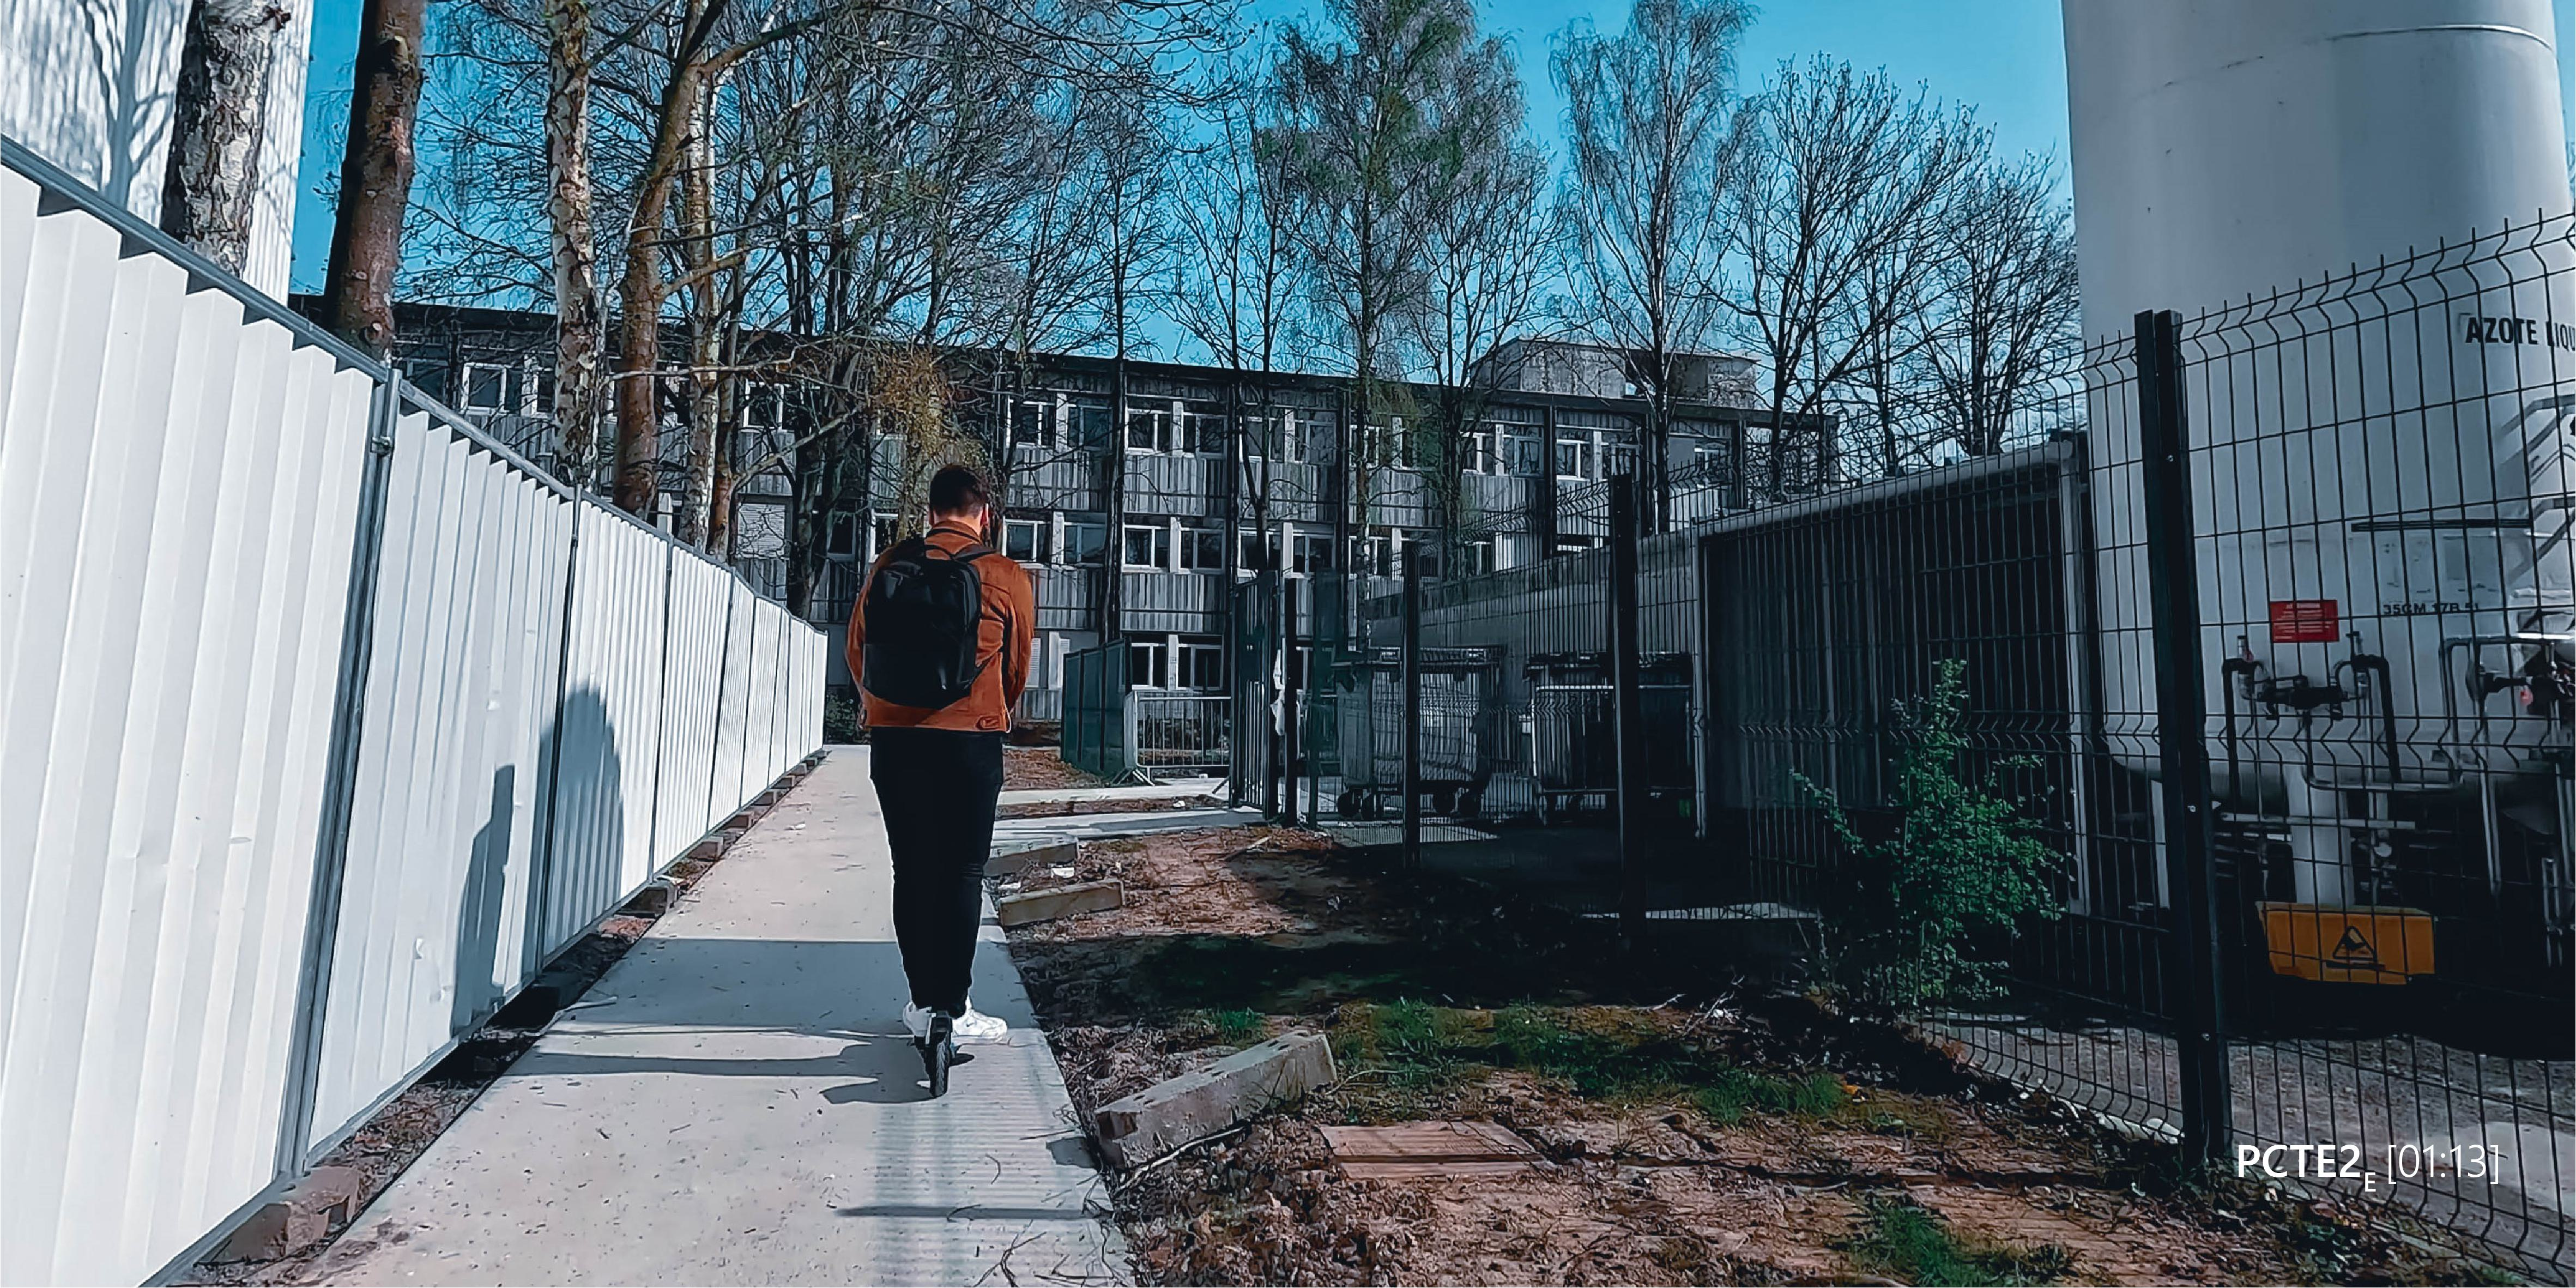
\includegraphics[width=0.75\columnwidth]{src/Figures/Annexes/Extrait_Video_PCTE2_Egress_3.jpg}}
        \vspace{5pt}
        \begin{flushright}\scriptsize{
        Auteur~: \textcolor{blue}{Dylan Moinse (2022)}
        }\end{flushright}
    \end{figure}

    % PCTE2 Photo Egress 4
    \begin{figure}[h!]\vspace*{4pt}
        \caption*{Extrait n°4 de la vidéo lors du trajet en diffusion (\(PCTE^{E}_{2}\))}
        \centerline{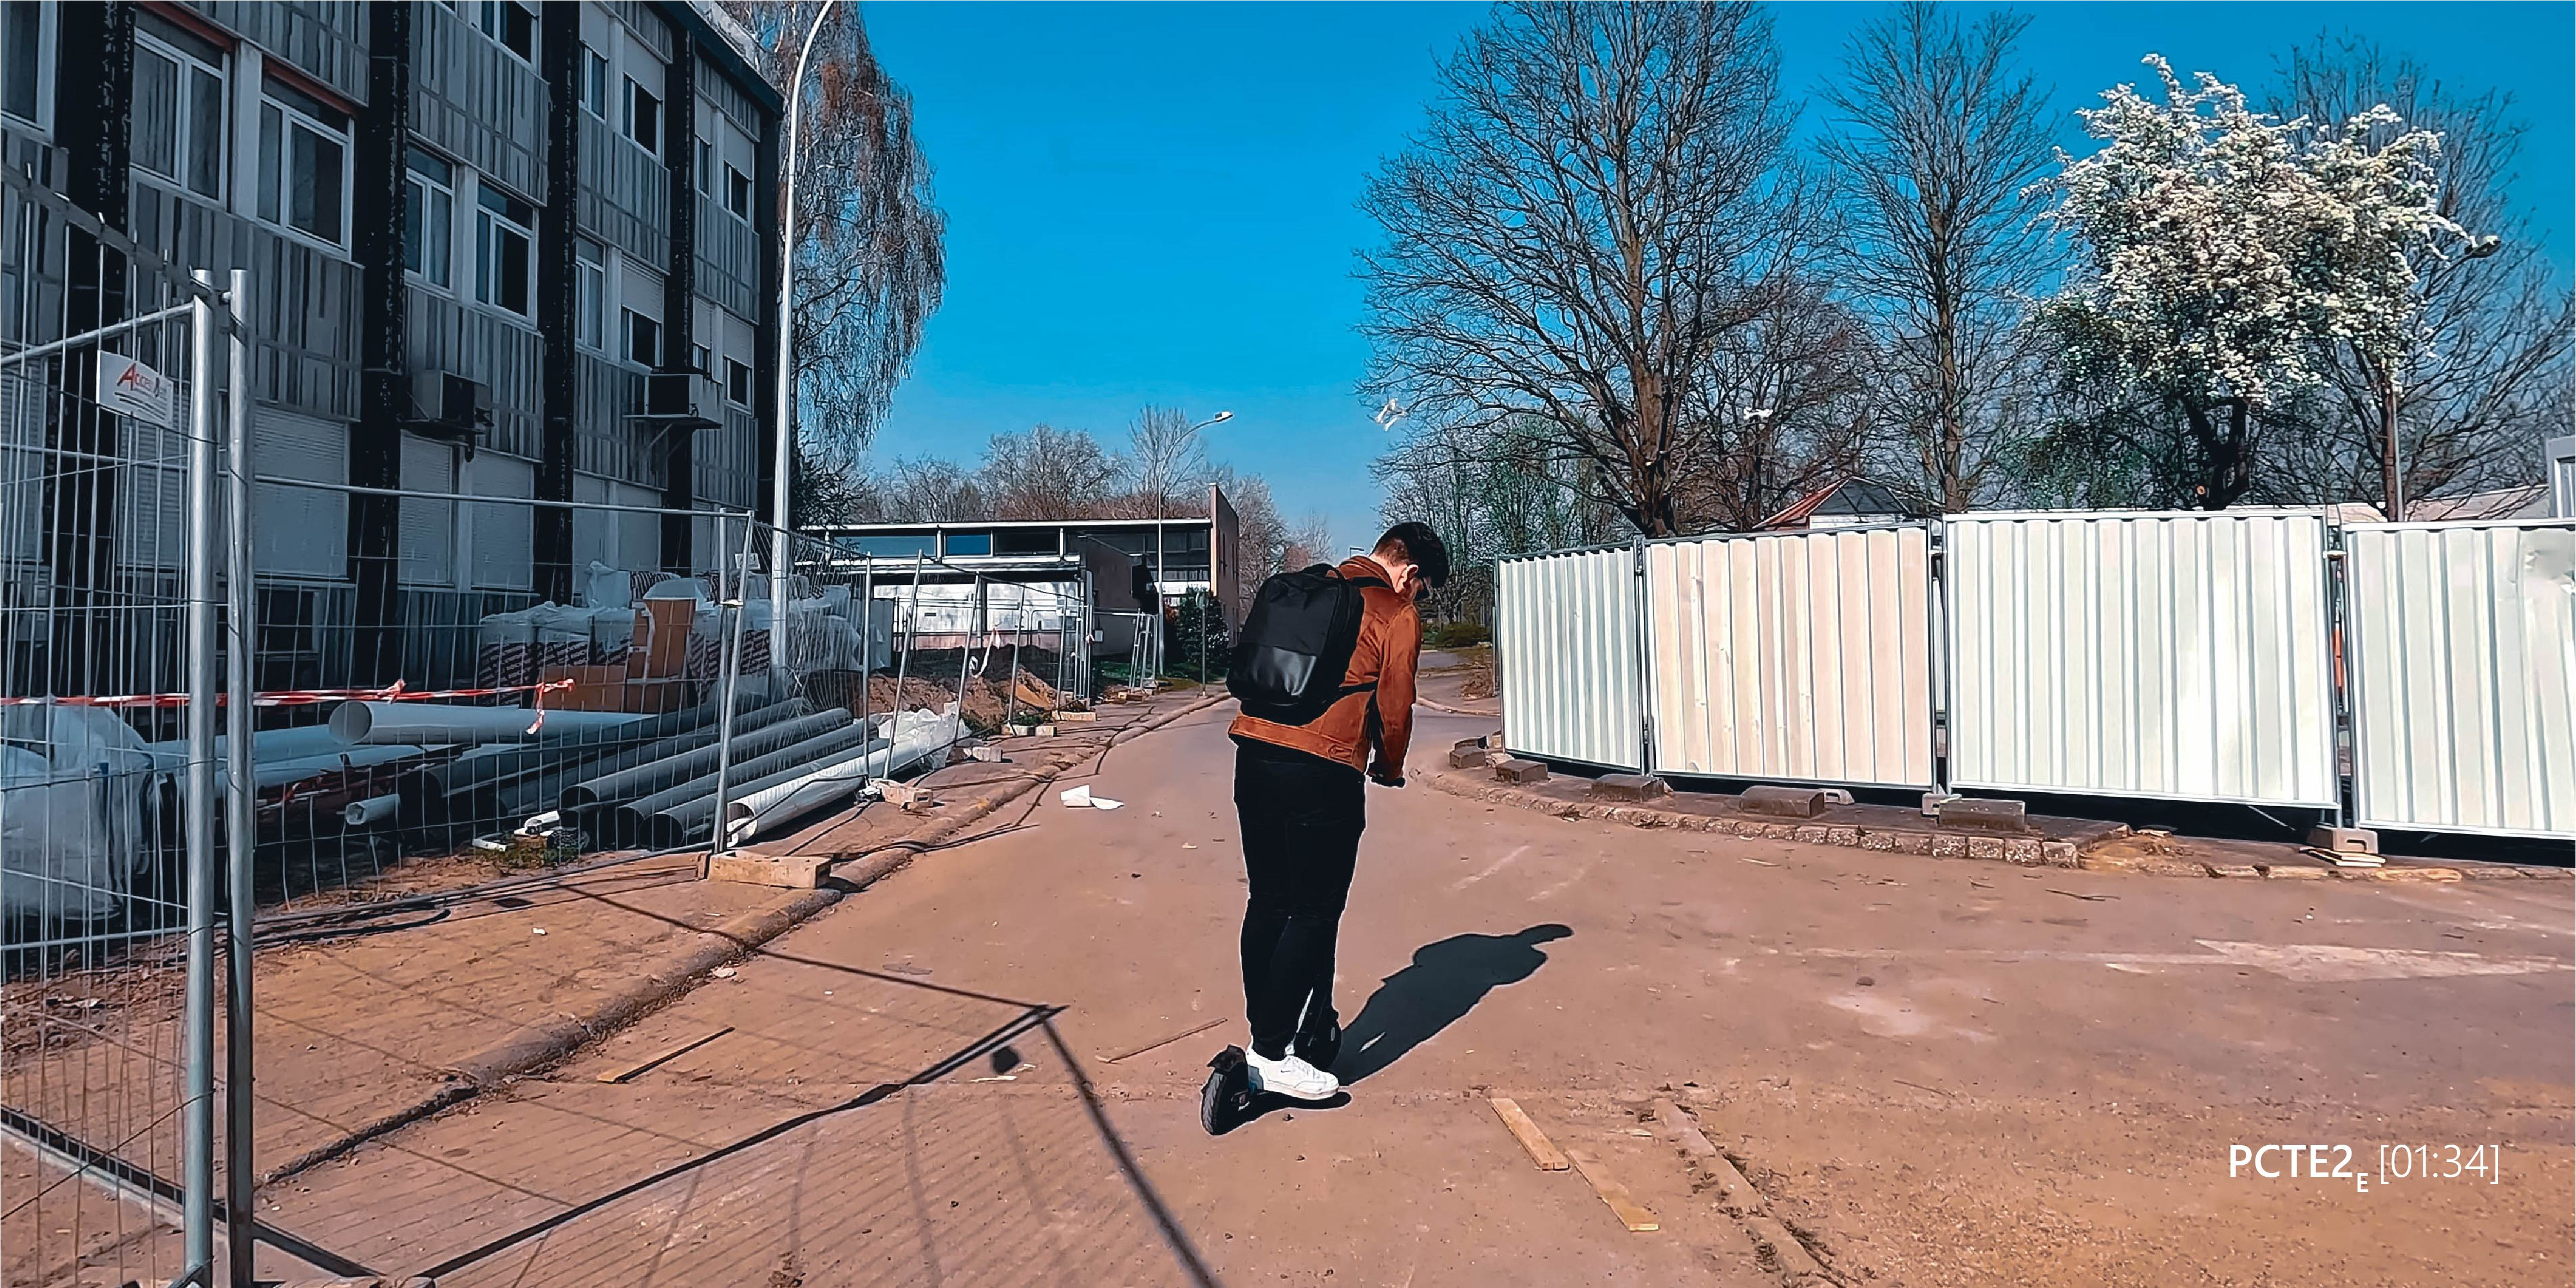
\includegraphics[width=0.75\columnwidth]{src/Figures/Annexes/Extrait_Video_PCTE2_Egress_4.jpg}}
        \vspace{5pt}
        \begin{flushright}\scriptsize{
        Auteur~: \textcolor{blue}{Dylan Moinse (2022)}
        }\end{flushright}
    \end{figure}

    % PCTE2 Photo Egress 5
    \begin{figure}[h!]\vspace*{4pt}
        \caption*{Extrait n°5 de la vidéo lors du trajet en diffusion (\(PCTE^{E}_{2}\))}
        \centerline{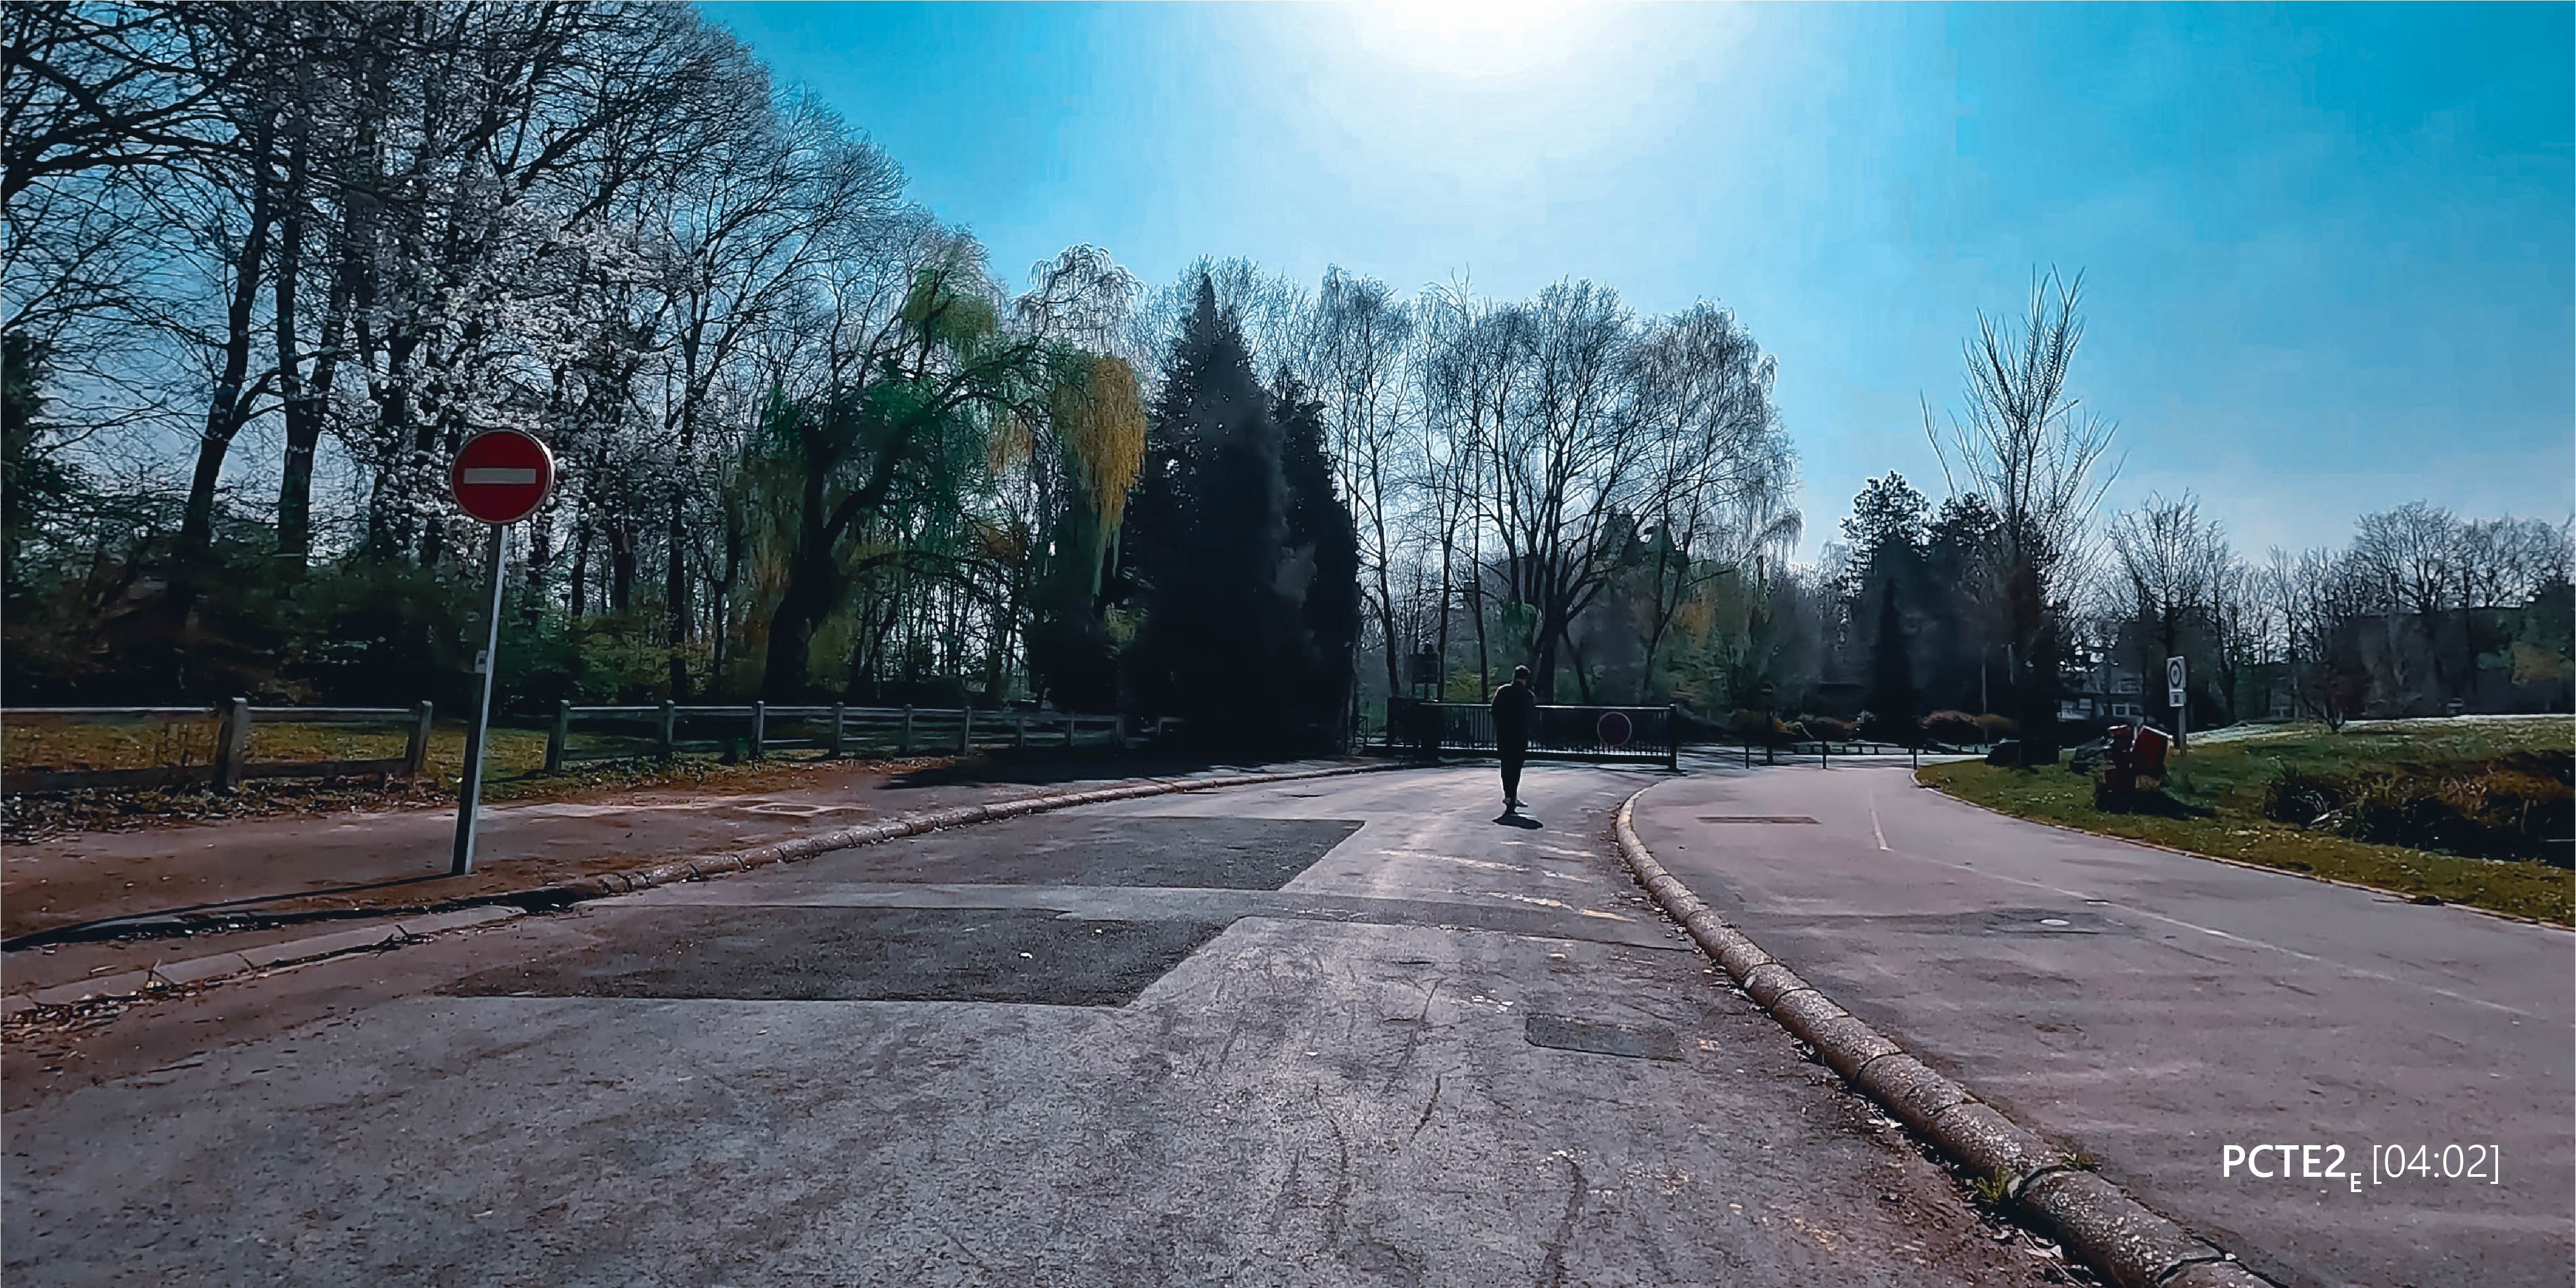
\includegraphics[width=0.75\columnwidth]{src/Figures/Annexes/Extrait_Video_PCTE2_Egress_5.jpg}}
        \vspace{5pt}
        \begin{flushright}\scriptsize{
        Auteur~: \textcolor{blue}{Dylan Moinse (2022)}
        }\end{flushright}
    \end{figure}

    % PCTE2 Photo Egress 6
    \begin{figure}[h!]\vspace*{4pt}
        \caption*{Extrait n°6 de la vidéo lors du trajet en diffusion (\(PCTE^{E}_{2}\))}
        \centerline{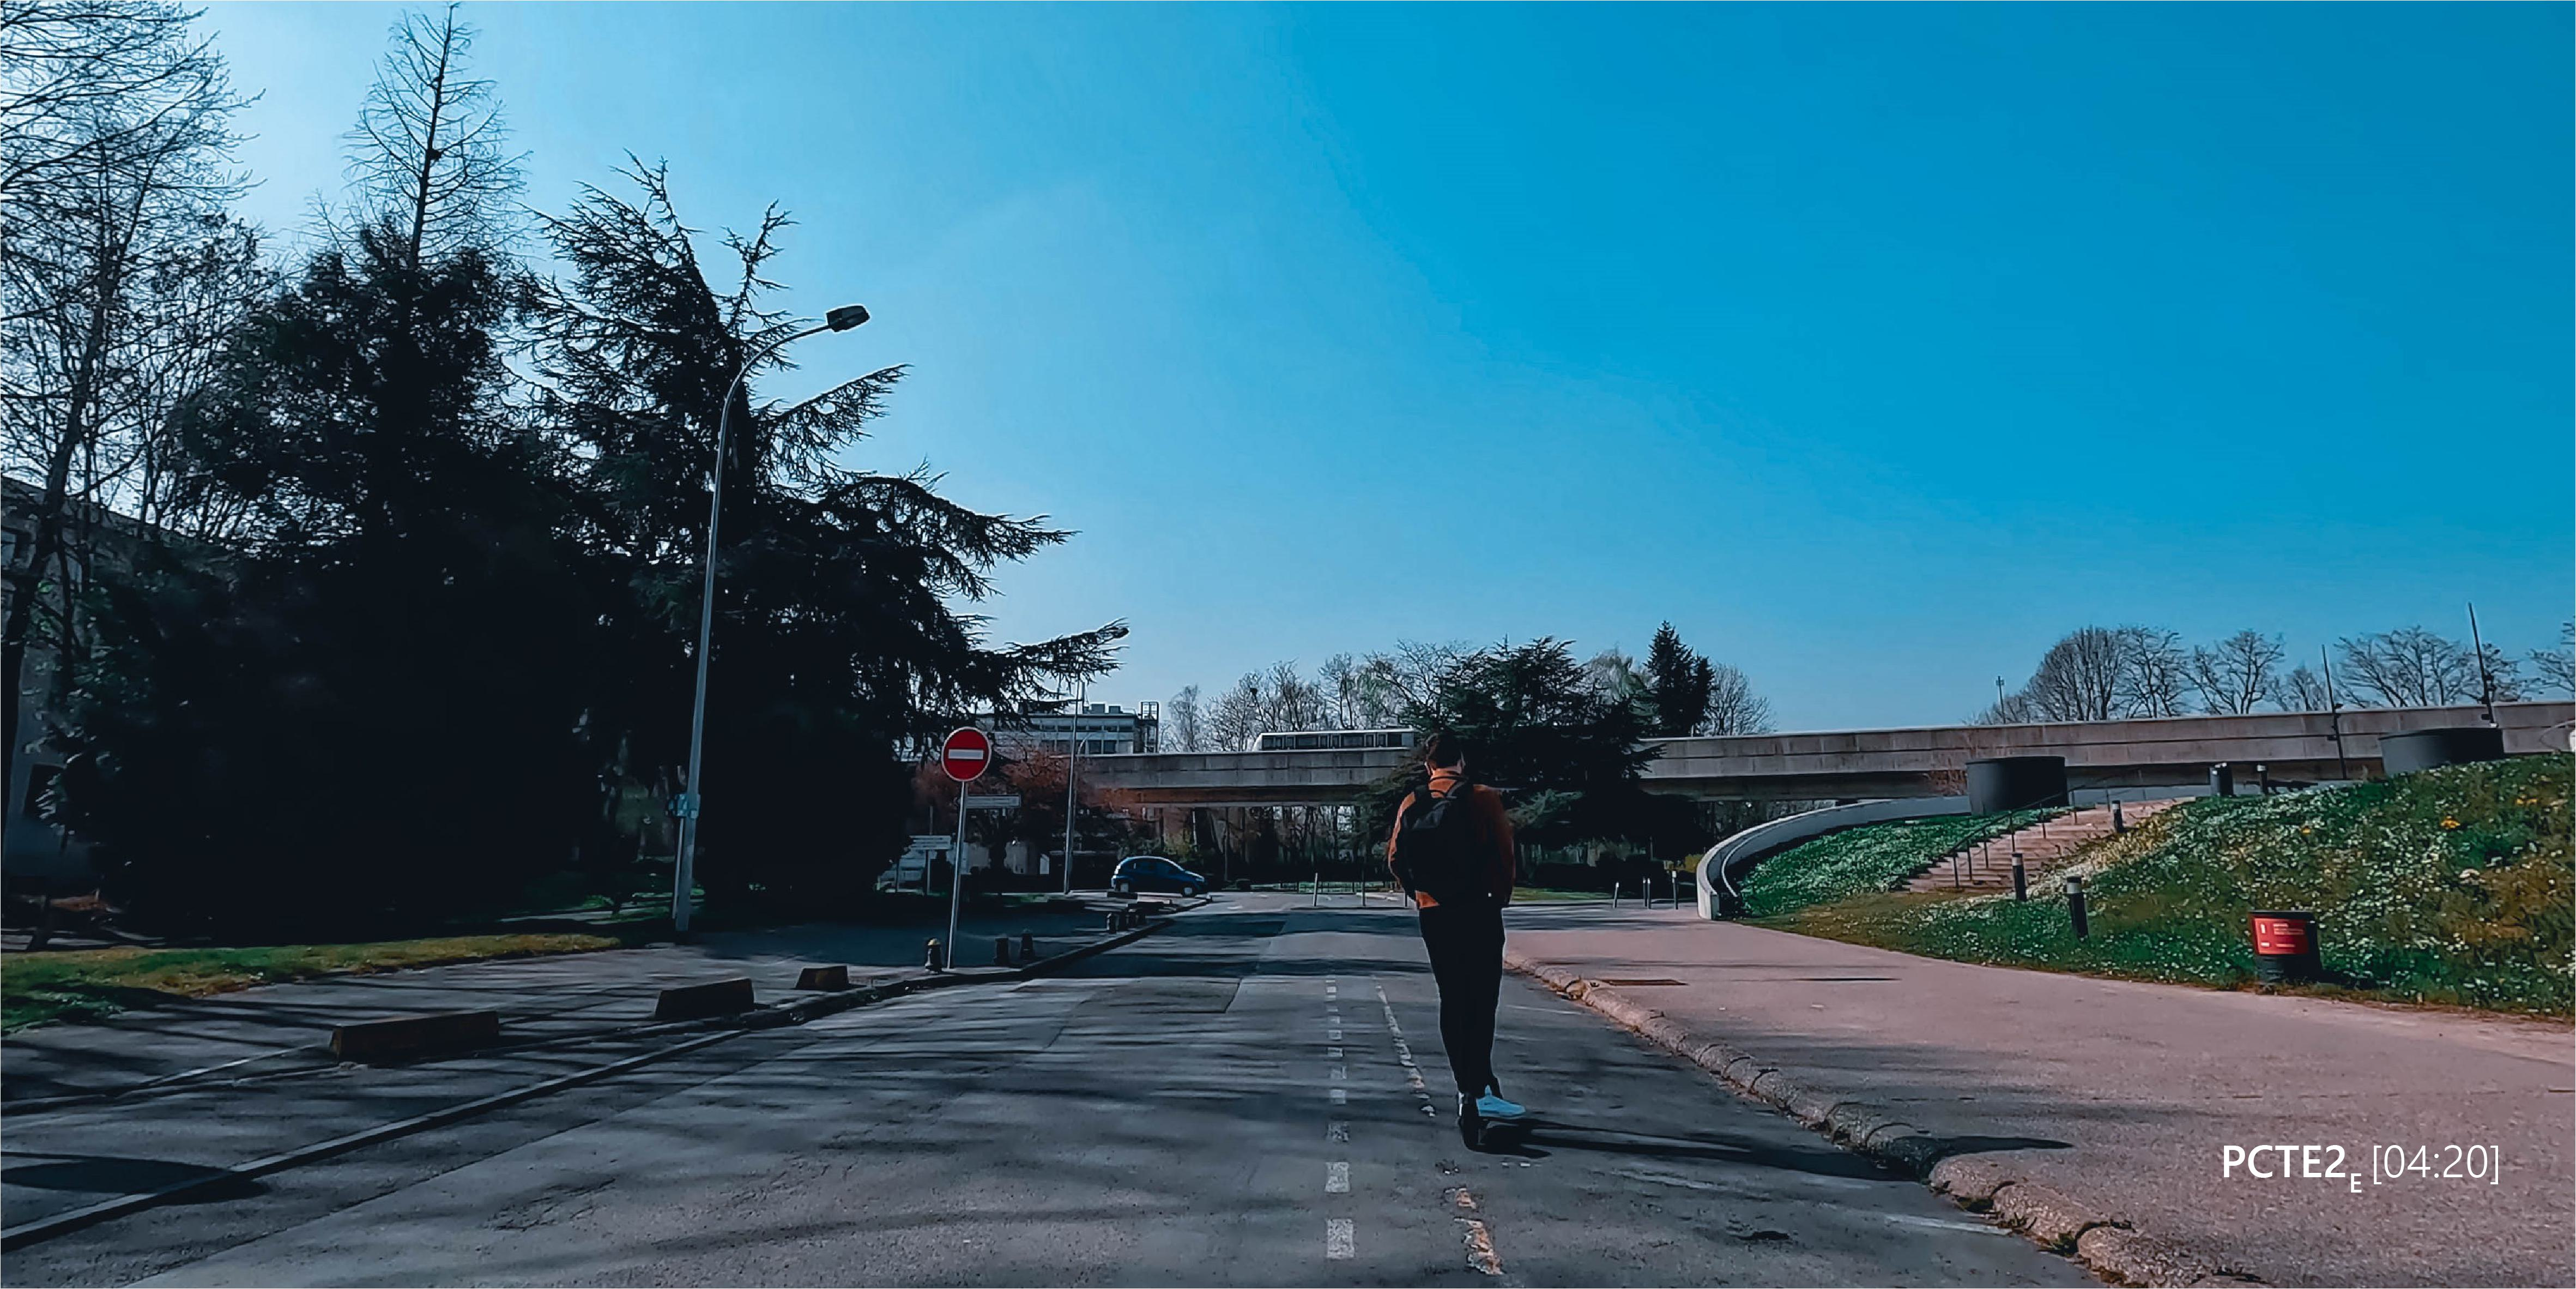
\includegraphics[width=0.75\columnwidth]{src/Figures/Annexes/Extrait_Video_PCTE2_Egress_6.jpg}}
        \vspace{5pt}
        \begin{flushright}\scriptsize{
        Auteur~: \textcolor{blue}{Dylan Moinse (2022)}
        }\end{flushright}
    \end{figure}

    % PCTE2 Photo Egress 7
    \begin{figure}[h!]\vspace*{4pt}
        \caption*{Extrait n°7 de la vidéo lors du trajet en diffusion (\(PCTE^{E}_{2}\))}
        \centerline{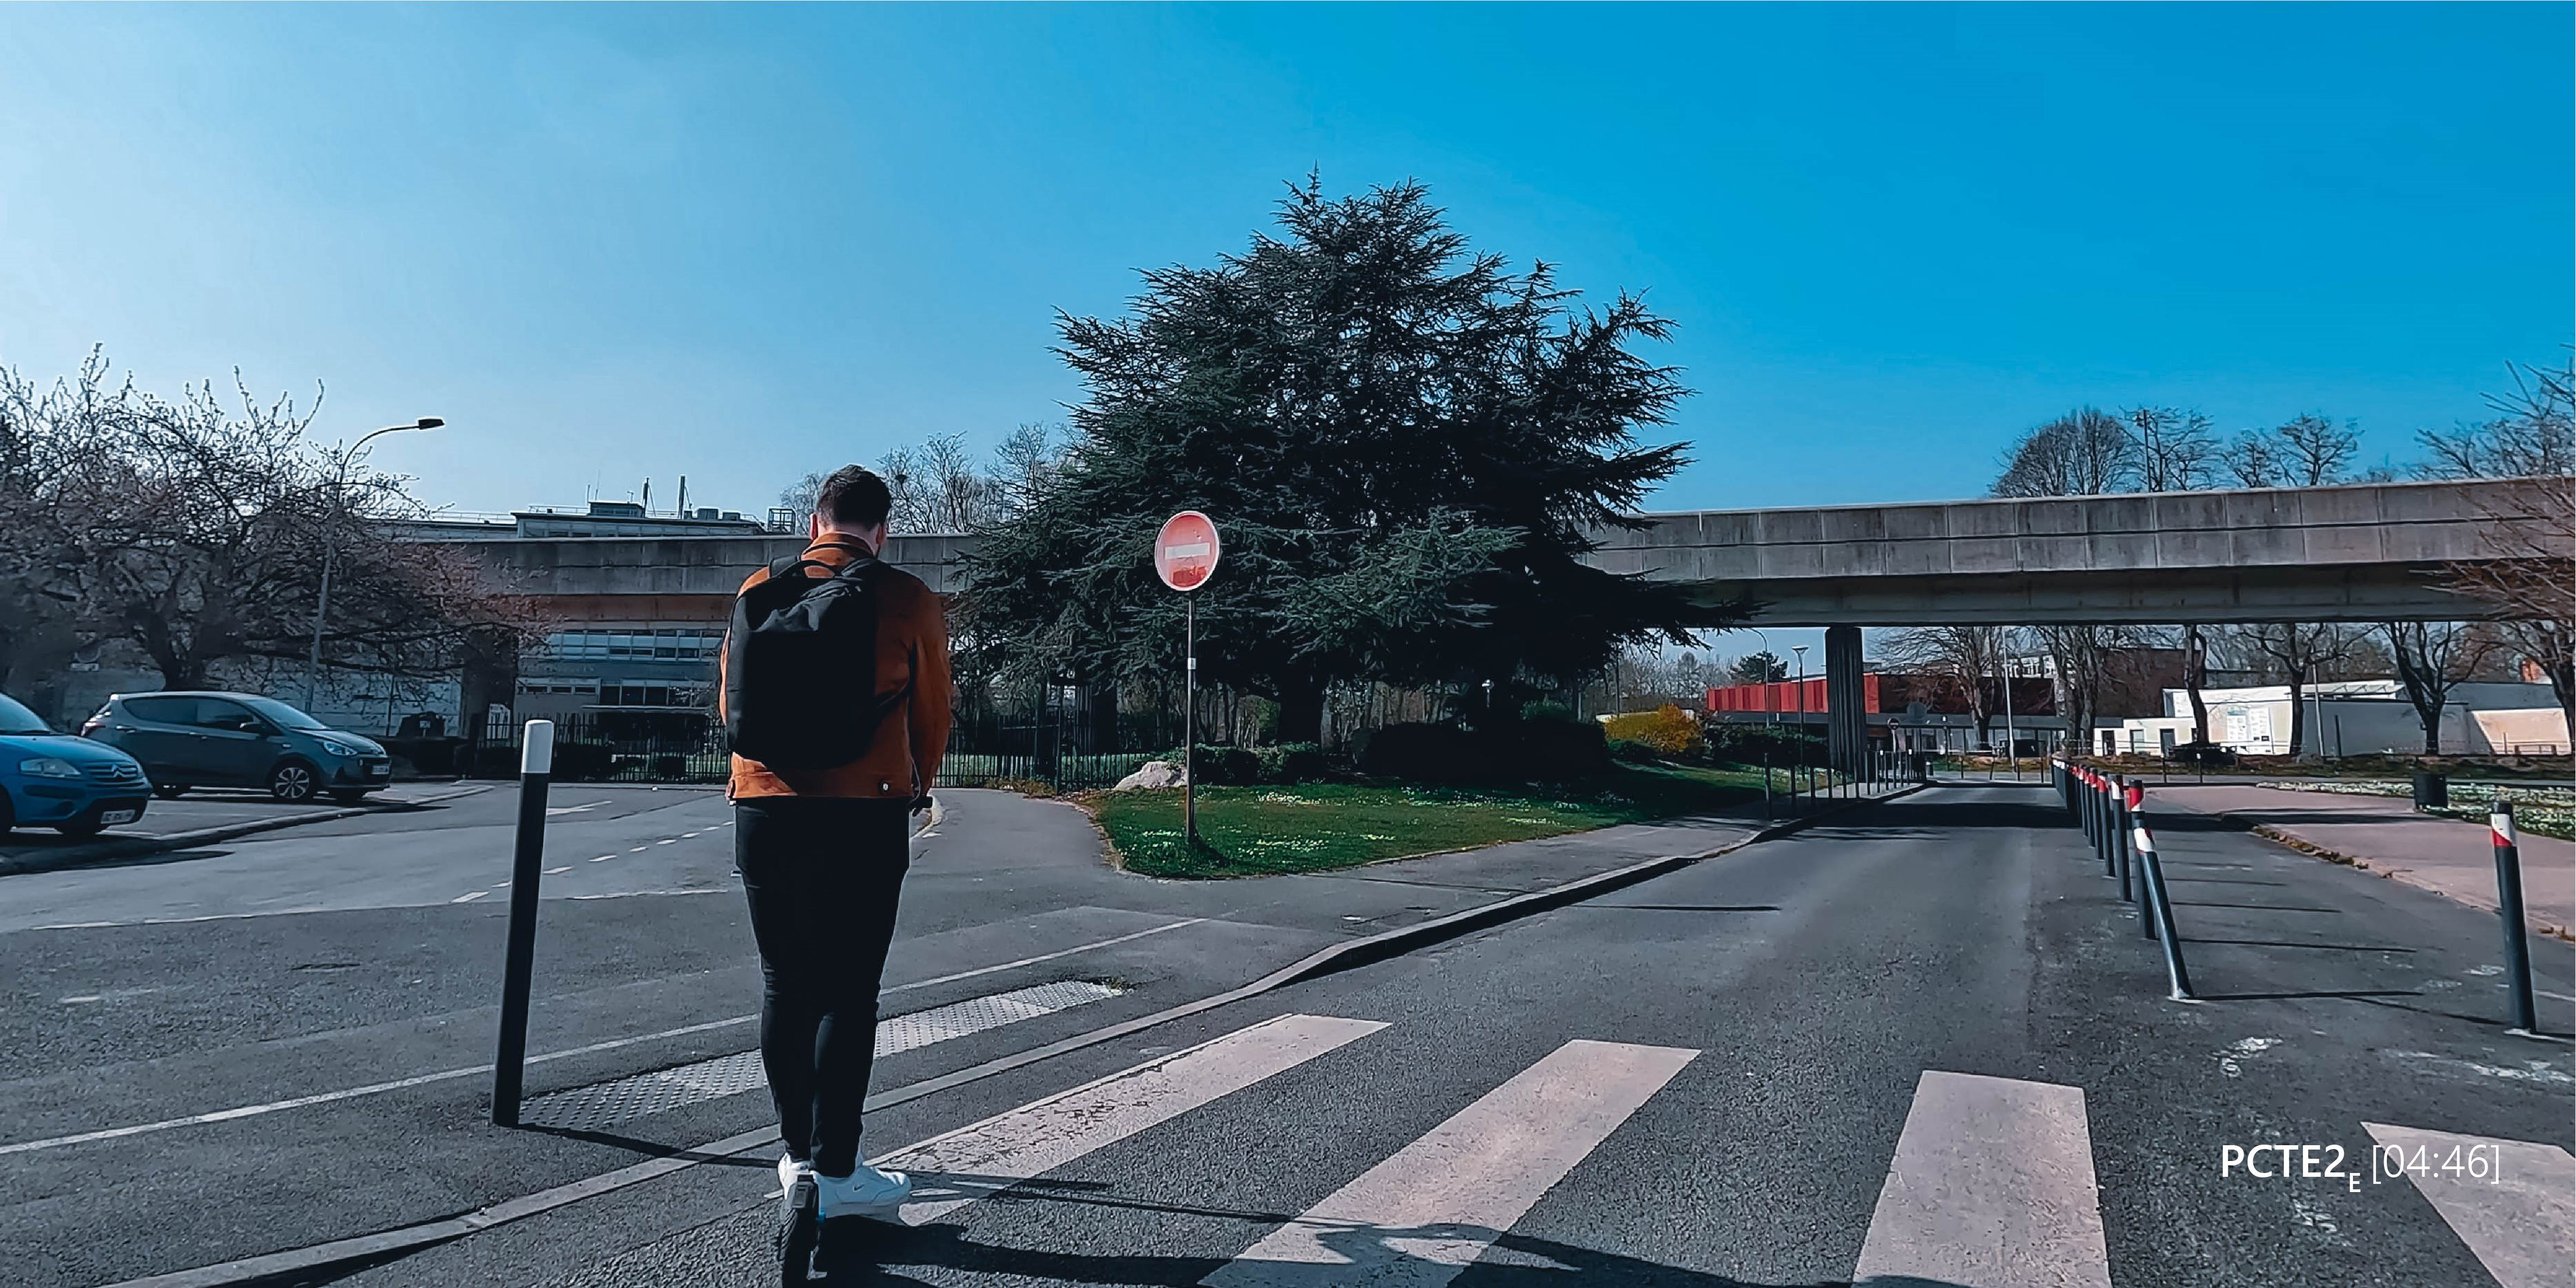
\includegraphics[width=0.75\columnwidth]{src/Figures/Annexes/Extrait_Video_PCTE2_Egress_7.jpg}}
        \vspace{5pt}
        \begin{flushright}\scriptsize{
        Auteur~: \textcolor{blue}{Dylan Moinse (2022)}
        }\end{flushright}
    \end{figure}

    % PCTE2 Photo Egress 8
    \begin{figure}[h!]\vspace*{4pt}
        \caption*{Extrait n°8 de la vidéo lors du trajet en diffusion (\(PCTE^{E}_{2}\))}
        \centerline{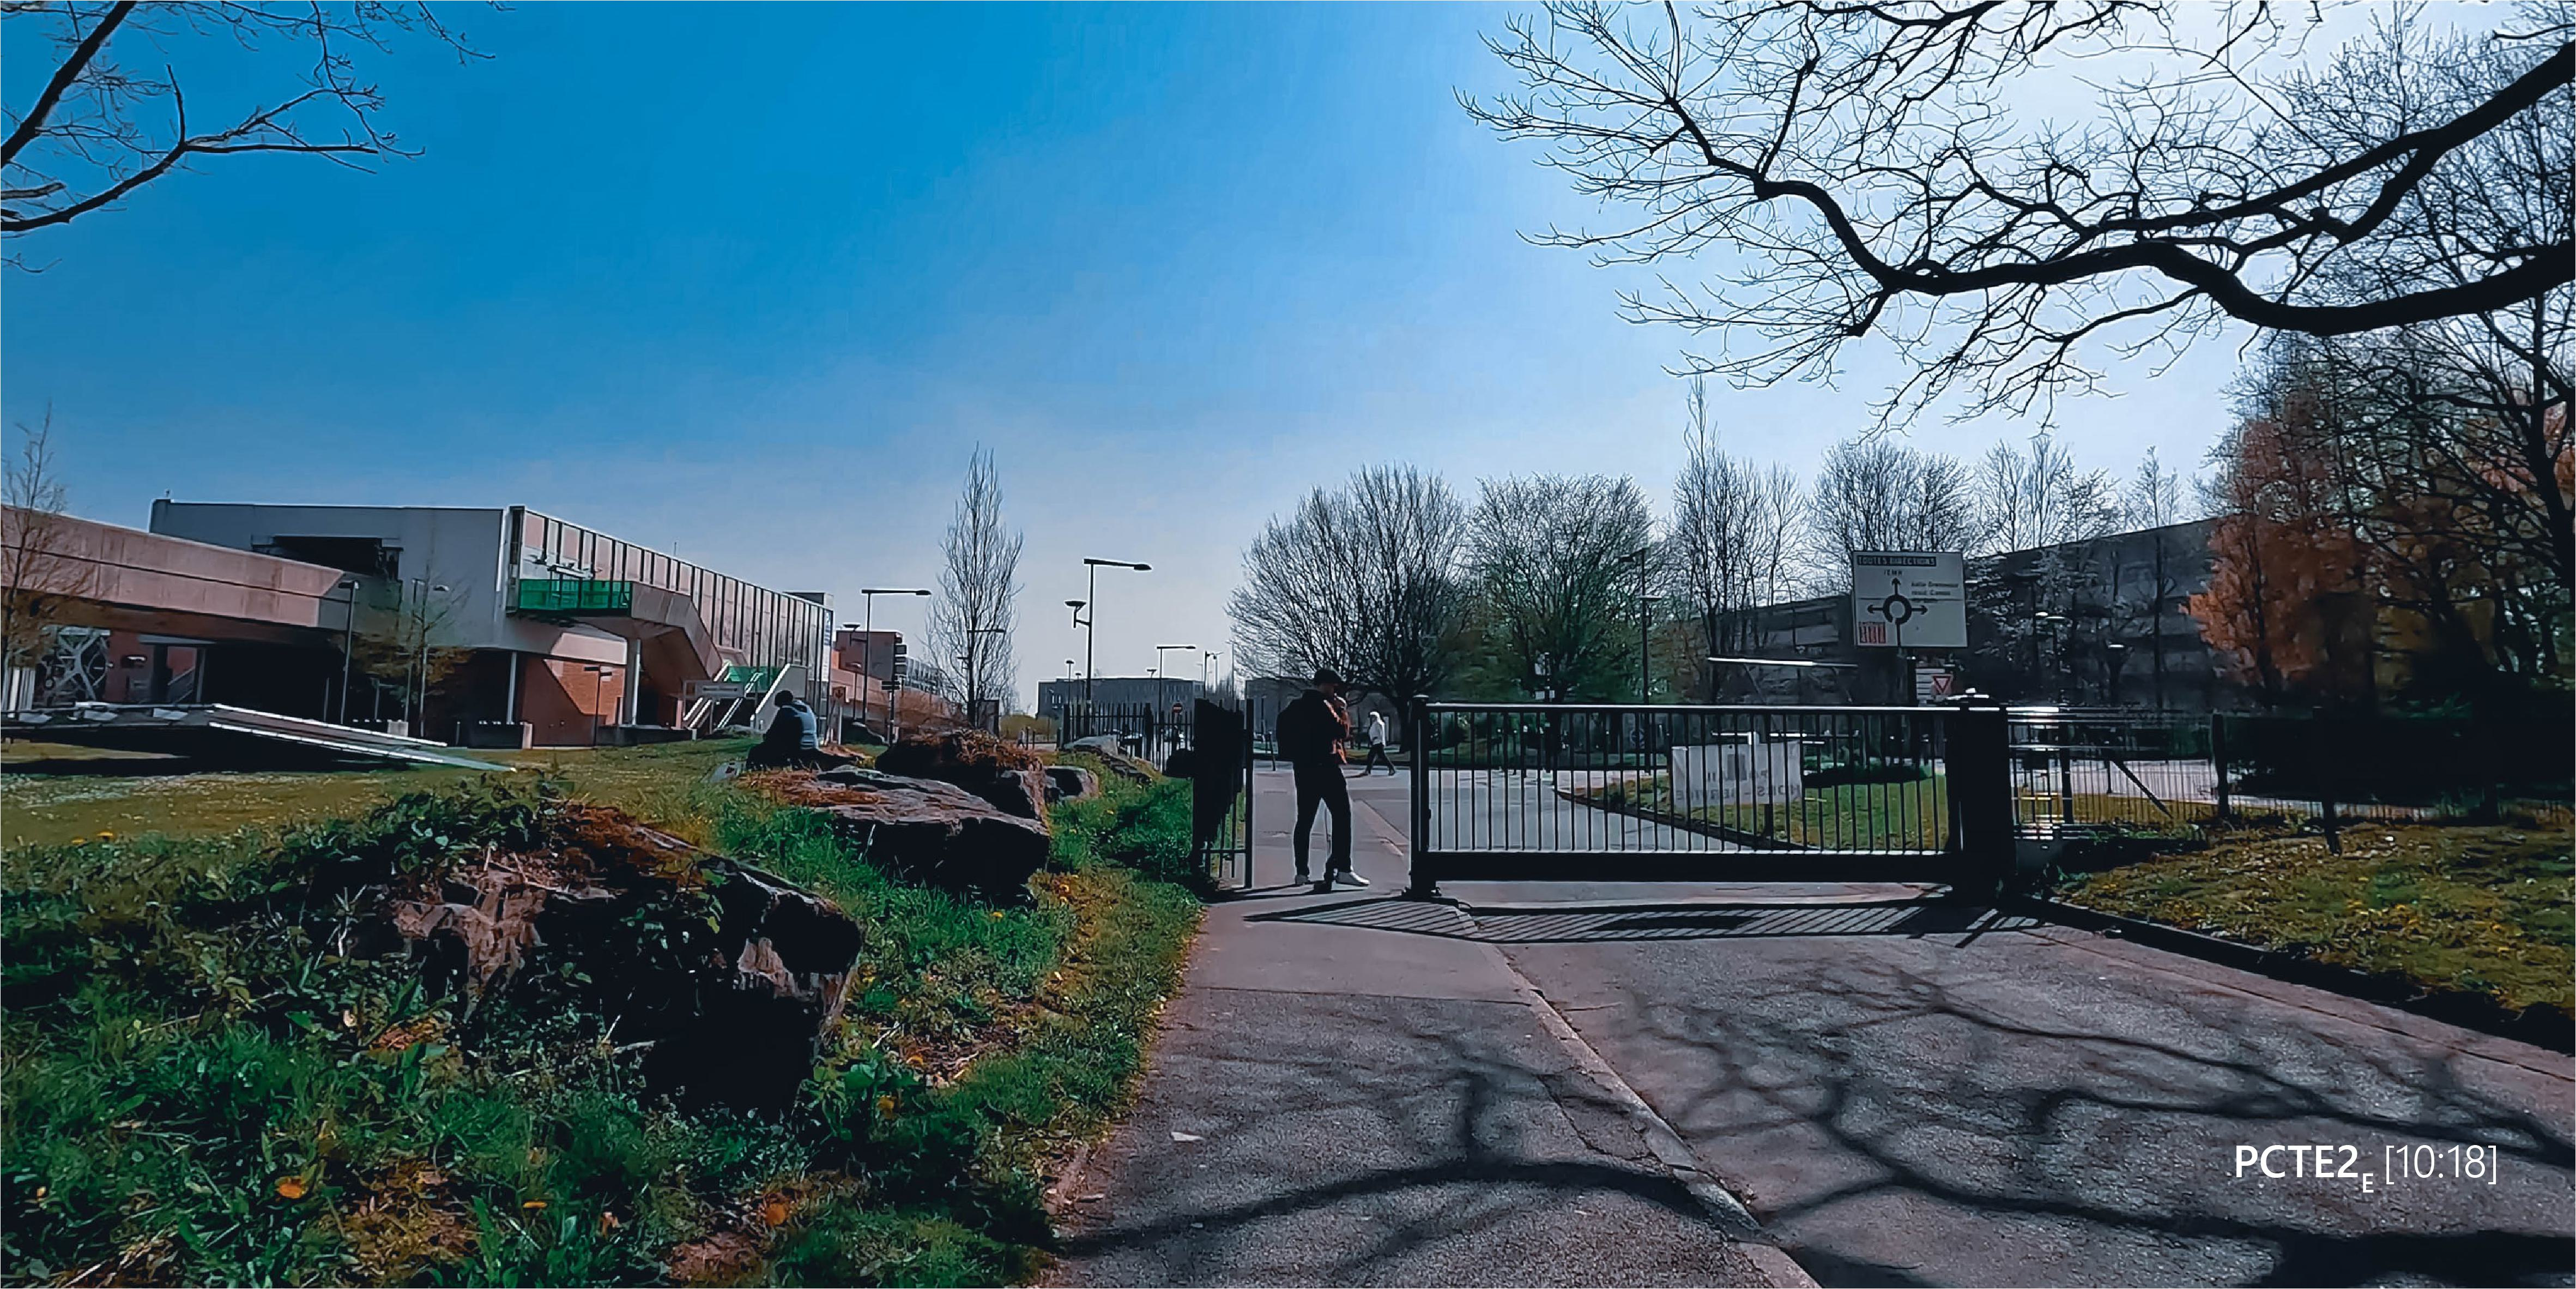
\includegraphics[width=0.75\columnwidth]{src/Figures/Annexes/Extrait_Video_PCTE2_Egress_8.jpg}}
        \vspace{5pt}
        \begin{flushright}\scriptsize{
        Auteur~: \textcolor{blue}{Dylan Moinse (2022)}
        }\end{flushright}
    \end{figure}

    % PCTE2 Photo Egress 9
    \begin{figure}[h!]\vspace*{4pt}
        \caption*{Extrait n°9 de la vidéo lors du trajet en diffusion (\(PCTE^{E}_{2}\))}
        \centerline{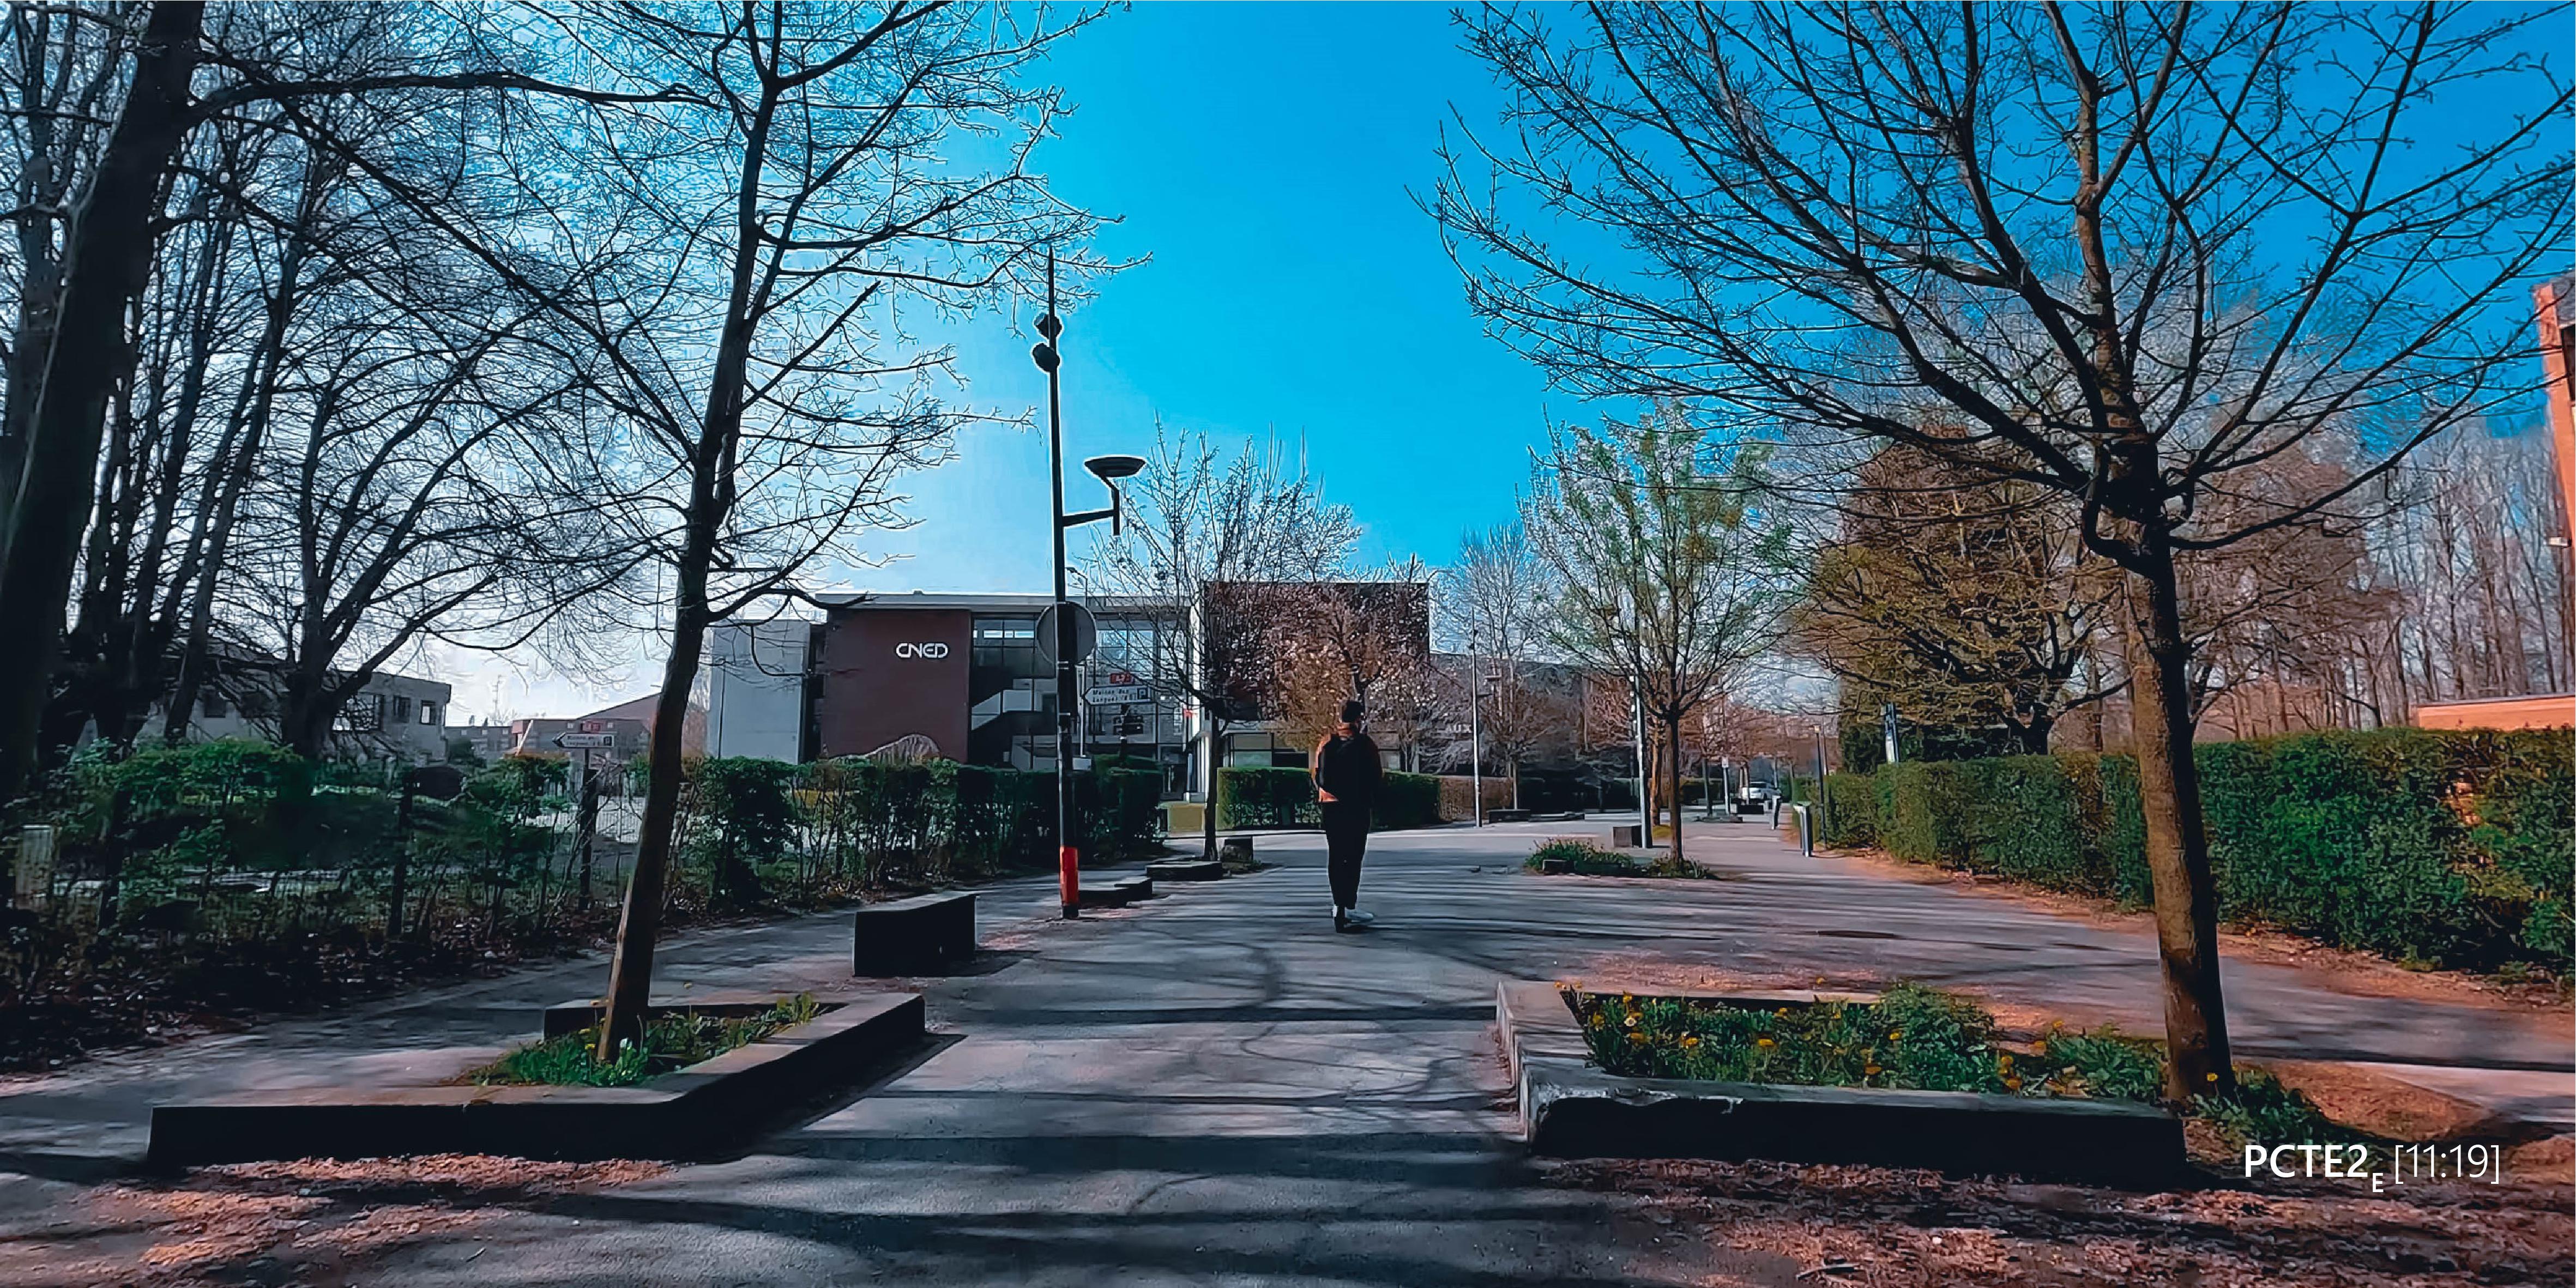
\includegraphics[width=0.75\columnwidth]{src/Figures/Annexes/Extrait_Video_PCTE2_Egress_9.jpg}}
        \vspace{5pt}
        \begin{flushright}\scriptsize{
        Auteur~: \textcolor{blue}{Dylan Moinse (2022)}
        }\end{flushright}
    \end{figure}